\documentclass[12pt]{book}
\usepackage[english]{babel}
\usepackage[utf8]{inputenc}
\usepackage[T1]{fontenc}
\usepackage{amsmath}
\usepackage{indentfirst}
\usepackage{graphicx}
\usepackage{gensymb}
\usepackage[colorinlistoftodos]{todonotes}
\usepackage{layout}
\usepackage{amssymb}	
\usepackage{pdfpages}
\usepackage{enumerate}
\usepackage{siunitx}
\usepackage{float}
\usepackage{adjustbox}
\usepackage{booktabs}
\usepackage{cancel}
\usepackage{tocloft}
\usepackage{setspace}	
\usepackage{subfig}
\usepackage{array,multirow}
\usepackage[left=2cm, right=2cm, top=2.5cm, bottom=2.5cm]{geometry}
\usepackage{longtable}
\usepackage{xcolor,colortbl}
\usepackage[pdftex,hidelinks]{hyperref}
\usepackage{tikz}
\usetikzlibrary{positioning,calc,3d,}
\usepackage{pgfplots}
\usepackage{tikz-3dplot}
\usepackage{slashbox}

\setlength{\arrayrulewidth}{1pt}

\newcommand{\idiii}[1]{%
	\pgfmathsetmacro{\idii}{#1-1}}

\newcolumntype{M}[1]{>{\raggedright\arraybackslash}m{#1\linewidth-2\tabcolsep - 1.25\arrayrulewidth}}
\newcolumntype{N}[1]{>{\centering\arraybackslash}m{#1\linewidth-2\tabcolsep - 1.25\arrayrulewidth}}

\definecolor{dkgreen}{RGB}{0,100,0}

\newcommand{\Thm}{\textbf{Theorem:} }
\newcommand{\Def}{\textcolor{dkgreen}{\textbf{Definition:}} }
\newcommand{\Proof}{\textcolor{blue}{\textbf{Proof:}} }
\newcommand{\Lemma}{\textcolor{red}{\textbf{Lemma:}} }

\setlength{\parskip}{6pt}
\setcounter{tocdepth}{2}

\begin{document}
\tableofcontents
\chapter{Stream Ciphers}
\section{What is cryptography about?}
\subsection{Course Overview}
\subsubsection{Course Objectives}
\begin{itemize}
	\item Learn how crypto primitives work
	\item Learn how to use them correctly and reason about security
\end{itemize}

\subsubsection{Crypto is everywhere}
\begin{itemize}
	\item Secure communication:
	\begin{itemize}
		\item web traffic: HTTPS
		\item wireless traffic: 802.11i WPA2, GSM, Bluetooth
	\end{itemize}
	
	\item Encrypting files on disk:
	\begin{itemize}
		\item EFS
		\item TrueCrypt
	\end{itemize}
	
	\item Content protection (e.g. DVD, Blu-ray):
	\begin{itemize}
		\item CSS (easy to brake)
		\item AACS
	\end{itemize}
	
	\item User authentication, and much much more.
\end{itemize}

\subsubsection{The web traffic, by HTTP, is protected by Secure Sockets Layer (SSL) / TLS.}
\begin{itemize}
	\item Two main parts:
	\begin{itemize}
		\item Handshake Protocol: Establish shared secret key using public-key cryptography ($2^{nd}$ part of course)
		\item Record Layer: Transmit data using shared secret key. Ensure confidentiality and integrity ($1^{st}$ part of course)
	\end{itemize}
\end{itemize}

\subsubsection{Building block: symmetric encryption}
\begin{center}
	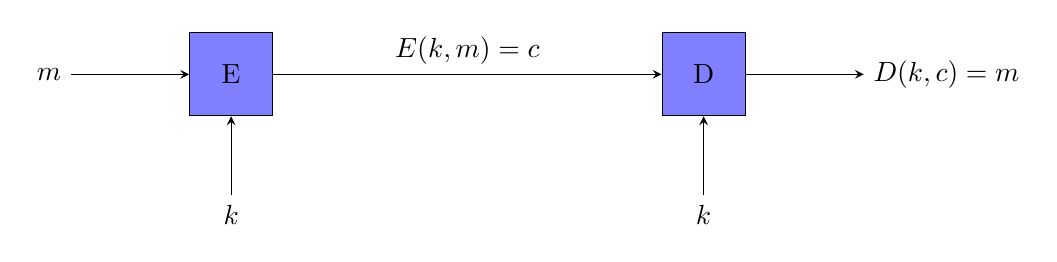
\begin{tikzpicture}
		\node[rectangle, fill=blue!50, draw=black, minimum width=30pt, minimum height = 30pt] (E) at (0,0) {E};
		\node[rectangle, fill=blue!50, draw=black, minimum width=30pt, minimum height = 30pt] (D) at (6,0) {D};
		\node[rectangle, left=1.5cm of E] (m) at (E.west) {$m$};
		\node[rectangle, right=1.5cm of D] (mout) at (D.east) {$D(k,c)=m$};
		\node[rectangle, below=1cm of E] (k1) at (E.south) {$k$};
		\node[rectangle, below=1cm of D] (k2) at (D.south) {$k$};
		\node[rectangle] (Ekm) at (3,0.3) {$E(k,m)=c$};
		
		\draw[-stealth] (E.east) -- (D.west);
		\draw[-stealth] (m.east) -- (E.west);
		\draw[-stealth] (D.east) -- (mout.west);
		\draw[-stealth] (k1.north) -- (E.south);
		\draw[-stealth] (k2.north) -- (D.south);
	\end{tikzpicture}
\end{center}Where $E$ is the encryption algorithm and $D$ is the decryption algorithm, $m$ is the message or plaintext and $c$ is the ciphertext. $k$ is the secret key and the pair $E$, $D$ is the cipher.

\textbf{Encryption algorithm is publicly known. Should never use a proprietary cipher.}

\subsubsection{Use Cases}
\begin{itemize}
	\item Single use key: (one time key)
	\begin{itemize}
		\item Key is only used to encrypt one message
		\begin{itemize}
			\item Encrypted email: new key generated for every email
		\end{itemize}
	\end{itemize}
	\item Multi use key: (many time key)
	\begin{itemize}
		\item Key used to encrypt multiple messages
		\begin{itemize}
			\item Encrypted files: same key used to encrypt many files
		\end{itemize}
		\item Need more machinery than for one-time key, to ensure security.
	\end{itemize}
\end{itemize}

\subsubsection{Things to remember}
\begin{itemize}
	\item Cryptography is:
	\begin{itemize}
		\item A tremendous tool
		\item The basis for many security mechanisms
	\end{itemize}
	\item Cryptography is not:
	\begin{itemize}
		\item The solution to all security problems
		\item Reliable unless implemented and used properly
		\item Something you should try to invent yourself, since there are many examples of broken ad-hoc designs
	\end{itemize}
\end{itemize}

\subsection{What is Cryptography?}
\subsubsection{Protocols}
Trusted authority takes inputs and generates an output in a trustworthy way.

\Thm Anything the can done with trusted authority can also be done without.

\subsubsection{A rigorous science}
\begin{itemize}
	\item The three steps in cryptography:
	\begin{itemize}
		\item Precisely specify threat model
		\item Propose a construction
		\item Prove that breaking construction under threat model will solve an underlying hard problem 
	\end{itemize}
\end{itemize}

\subsection{History of Cryptography}
\subsubsection{Few Historic Examples}
\begin{enumerate}
	\item Substitution Cipher
	\begin{center}
		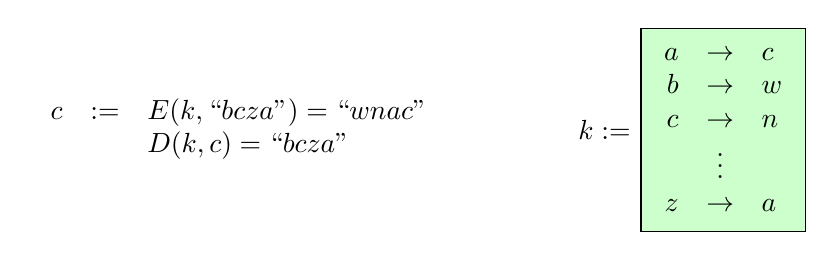
\begin{tikzpicture}
			\node[rectangle] (k) at (0,0){$k:=$};
			\node[rectangle, draw=black, fill=green!20, anchor=west] (ks) at (k.east) {$\begin{array}{rcl}
					a&\rightarrow&c\\
					b&\rightarrow&w\\
					c&\rightarrow&n\\
					&\vdots&\\
					z&\rightarrow&a\\
				\end{array}$};
			\node[rectangle, left=1.5cm of k, anchor=east] (c) at (k.west){$\begin{array}{rcl}
					c&:=&E(k,``bcza")=``wnac"\\
					&&D(k,c)=``bcza"
				\end{array}$};
		\end{tikzpicture}
	\end{center}
	\item Ceaser Cipher (no key because the key is fixed)
	\begin{center}
		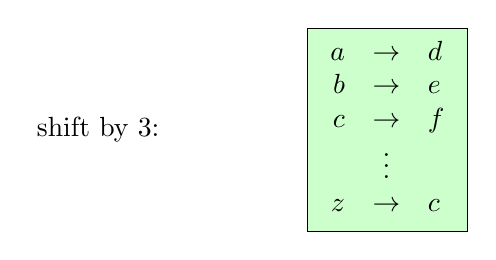
\begin{tikzpicture}
			\node[rectangle] (k) at (0,0){};
			\node[rectangle, draw=black, fill=green!20, anchor=west] (ks) at (k.east) {$\begin{array}{rcl}
					a&\rightarrow&d\\
					b&\rightarrow&e\\
					c&\rightarrow&f\\
					&\vdots&\\
					z&\rightarrow&c\\
				\end{array}$};
			\node[rectangle, left=1.5cm of k, anchor=east] (c) at (k.west){shift by 3:};
		\end{tikzpicture}
	\end{center}
	\item Vigener cipher (16'th century, Rome)
	$$\begin{array}{rccl}
		k&=&\mathtt{C\ R\ Y\ P\ T\ O\ C\ R\ Y\ P\ T\ O\ C\ R\ Y\ P\ T}&\\
		&&&(+mod\ 26)\\
		m&=&\mathtt{W\ H\ A\ T\ A\ N\ I\ C\ E\ D\ A\ Y\ T\ O\ D\ A\ Y}&\\[0cm]
		&&\mathtt{----------------}&\\[0cm]
		c&=&\mathtt{Z\ Z\ Z\ J\ U\ C\ L\ U\ D\ T\ U\ N\ W\ G\ C\ Q\ S}&
	\end{array}$$
	\item Rotor machines (1870-1943): for example, the Herbern machine (single rotor), where the substitution table rotates every usage.
\end{enumerate}
\subsubsection{How to break a substitution cipher?}
\begin{enumerate}
	\item Use frequency of English letters
	\begin{center}
		``e'': 12.7\%, ``t'': 9.1\%, ``a'': 8.1\%
	\end{center}
	\item Use frequency of pairs of letters (digrams)
	\begin{center}
		``he'', ``an'', ``in''. ``th''
	\end{center}
\end{enumerate}

The substitution cipher is vulnerable to the worse type of attack: Cipher Text only attack (\textbf{CT only attack}). Just given the CT,  the attacker can recover the decryption key and, therefore, recover the original plaintext.

\subsubsection{How to break the Vigener cipher?}
We must assume we know the length of the key. Then, we must break the cipher text into groups of the same length. Then, we see the first letter of the CT, and we know the letter used is the same to encrypt the plain text every first letter of the group. Then, we suppose that the plain text is composed with most common letters.

\subsubsection{Data Encryption Standard}
DES: \#keys=$2^{56}$\footnote{\# is number of.}, block size = 64 bits\\
Today: AES (2001), Salsa20 (2008), and others.

\newpage
\section{Crash course in discrete probability}
\subsection{Discrete Probability}
Let U be a finite set (e.g. $U=\{0,1\}^{n}$, for example: $\{0,1\}^{2}=\{00,01,10,11\}$).

\subsubsection{Probability Distribution}
\Def Probability distribution P over U is a function $P: U\rightarrow [0,1]$ such that $\sum\limits_{x\in U}P(x)=1$.

Examples:
\begin{enumerate}
	\item Uniform distribution: for all $x \in U: P(x)=1/|U|$, where $|U|$ is the size of the universe U or the number of elements of U.
	\item Point distribution at $x_{0}$: $P(x_{0}) = 1,\ \forall x\neq x_{0}:\ P(x)=0$.
\end{enumerate}
We can represent the entire distribution of a set as a vector: $$Distribution\ vector:\ \left(P(x_{1}), P(x_{2}), \cdots, P(x_{n})\right)$$

\subsubsection{Events}
For a set $A\subseteq U:\ \ \ Pr[A]=\sum\limits_{x\in A}P(x)\ \in[0,1]$, where $Pr[U]=1$.

\Def The set A is called an event. And the probability of an event A is $Pr[A]$.

Example: Let $U=\{0,1\}^{8}$. Let $A=\{\text{all }x\text{ in }U\text{ such that }lsb_{2}(x)=11\}\subseteq U$. For the uniform distribution on $\{0,1\}^{8}$: $Pr[A]=\frac{1}{4}$.

\subsubsection{The union bound}
For events $A_{1}$ and $A_{2}$, both $\subseteq U$.

\Def $Pr[A_{1}\cup A_{2}]\leq Pr[A_{1}]+Pr[A_{2}]$. If $A_{1}\cap A_{2}=\varnothing\Rightarrow Pr[A_{1}\cup A_{2}]=Pr[A_{1}]+Pr[A_{2}]$.

Example: Let $A_{1}=\{\text{all }x\text{ in }\{0,1\}^{n}\text{ s.t }lsb_{2}(x)=11\}$ and $A_{2}=\{\text{all }x\text{ in }\{0,1\}^{n}\text{ s.t }msb_{2}(x)=11\}$. Then, we know that $Pr[lsb_{2}(x)==1\ or\ msb_{2}(x)=11]=Pr[A_{1}\cup A_{2}]\leq \frac{1}{4}+\frac{1}{4}=\frac{1}{2}$.

\subsubsection{Random Variables}
\Def A random variable $X$ is a function $X:U \rightarrow V$.

Example: $X:\{0,1\}^{n}\rightarrow\{0,1\}$ such that $X(y)=lsb(y)\ \in\{0,1\} $. For the uniform distribution on $U$: $$Pr[X=0]=\frac{1}{2},\ Pr[X=1]=\frac{1}{2}$$.

More generally: random variables $X$ induces a distribution on $V$: $Pr[X=v]:=Pr[X^{-1}(v)]$.

\subsubsection{The uniform random variable}
Let $U$ be some set, e.g. $U=\{0,1\}^{n}$.

\Def We write $r\xleftarrow{R} U$ to denote a uniform random variable $r$ over $U$. Then $$\forall a\in U:\ Pr[r=a]=\frac{1}{|U|}$$
Formally, $r$ is the identity function: $r(x)=x,\ \forall x\in U$.

Example: Let $r$ be a uniform random variable on $\{0,1\}^{2}$. Define the random variable $X=r_{1}+r_{2}$, where $r_{1}$ and $r_{2}$ are the first and second bits of $r$, respectively. Then $Pr[X=2]=\frac{1}{4}$.

\subsubsection{Randomized algorithms}
In the deterministic algorithms, an input $m$ always produces the same output $y$: $y\leftarrow A(m)$.
\begin{center}
	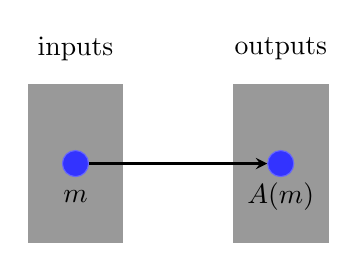
\begin{tikzpicture}
		\node [rectangle, draw=gray!80, fill=gray!80, minimum width=1.2cm, minimum height=2cm] (i) at (0,0){};
		\node [rectangle, draw=gray!80, fill=gray!80, minimum width=1.2cm, minimum height=2cm, shift={(2,0)}] (o) at (i.east){};
		
		\node [circle, draw=blue!60, fill=blue!80, minimum size=0.1cm] (m) at (i.center) {};
		\node [circle, draw=blue!60, fill=blue!80, minimum size=0.1cm] (Am) at (o.center) {};
		
		\node[shift={(0,-.25)}] (mt) at (m.south) {$m$};
		\node[shift={(0,-.25)}] (Amt) at (Am.south) {$A(m)$};
		
		\node [shift={(0,0.45)}] (in) at (i.north) {inputs};
		\node [shift={(0,0.45)}] (ou) at (o.north) {outputs};
		
		\draw[-stealth, thick] (m.east)--(Am.west);
	\end{tikzpicture}
\end{center}
In the randomized algorithms, an input $m$ produces different outputs every time it runs: $y\leftarrow A(m;r)$ where $r\xleftarrow{R}\{0,1\}^{n}$.
\begin{center}
	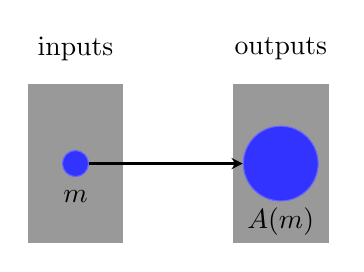
\begin{tikzpicture}
		\node [rectangle, draw=gray!80, fill=gray!80, minimum width=1.2cm, minimum height=2cm] (i) at (0,0){};
		\node [rectangle, draw=gray!80, fill=gray!80, minimum width=1.2cm, minimum height=2cm, shift={(2,0)}] (o) at (i.east){};
		
		\node [circle, draw=blue!60, fill=blue!80, minimum size=0.1cm] (m) at (i.center) {};
		\node [circle, draw=blue!60, fill=blue!80, minimum size=0.95cm] (Am) at (o.center) {};
		
		\node[shift={(0,-.25)}] (mt) at (m.south) {$m$};
		\node[shift={(0,-.25)}] (Amt) at (Am.south) {$A(m)$};
		
		\node [shift={(0,0.45)}] (in) at (i.north) {inputs};
		\node [shift={(0,0.45)}] (ou) at (o.north) {outputs};
		
		\draw[-stealth, thick] (m.east)--(Am.west);
	\end{tikzpicture}
\end{center}
A random algorithm can be defined as $$y\xleftarrow{R}A(m)$$
The encryption of a message with random keys fits in the definition of randomized algorithms.

\subsubsection{Independence}
\Def Events $A$ and $B$ are independent if $Pr[A\ and\ B]=Pr[A]\cdot Pr[B]$.

\Def Random variables $X,\ Y$ taking values in $V$ are independent if $\forall a,b\in V:Pr[X=a\ and\ Y=b] = Pr[X=a]\cdot Pr[Y=b]$.

Example: $U=\{0,1\}^{2}=\{00,01,10,11\}$ and $r\xleftarrow{R}U$. Define r.v. $X$ and $Y$ as: $X=lsb(r),\ Y=msb(r)$. $$Pr[X=0\ and\ Y=0]=Pr[r=00]=\frac{1}{4}=Pr[X=0]\cdot Pr[Y=0]$$The same happens with the other elements of $U$.

\subsubsection{Review: XOR}
XOR of two strings in $\{0,1\}^{n}$ is their bit-wise addition mod 2.
\begin{table}[!h]
	\centering
	\begin{tabular}{cc|c}
		$X$&$Y$&$X\oplus Y$\\\hline
		0&0&0\\
		0&1&1\\
		1&0&1\\
		1&1&0
	\end{tabular}
\end{table}

Example:
\begin{center}
	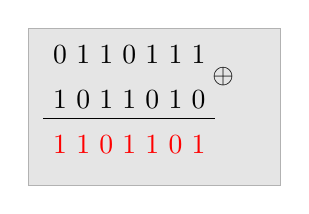
\begin{tikzpicture}
		\node[rectangle, draw=gray!60, fill=gray!20, anchor=north west, minimum width=3.2cm, minimum height=2cm] (box) at (0,0) {};
		\node[rectangle, anchor=north west, shift={(0.2,-0.1)}] (1) at (0,0){0 1 1 0 1 1 1};
		\node[rectangle, anchor=north west, shift={(0,-0.1)}] (2) at (1.south west){1 0 1 1 0 1 0};
		\draw[shift={(0,-0.1)}] (2.south west)--(2.south east);
		\node[rectangle, anchor=north west, shift={(0,-0.1)}] (r) at (2.south west){\textcolor{red}{1 1 0 1 1 0 1}};
		\node[shift={(0.1, -0.05)}] (mais) at (1.south east){$\oplus$};
	\end{tikzpicture}
\end{center}

\subsubsection{An important property of XOR}
\Thm Let $Y$ be a random variable over $\{0,1\}^{n}$, $X$ an independent uniform variable on $\{0,1\}^{n}$. Then $Z:=Y\oplus X$ is uniform variable on $\{0,1\}^{n}$.

\Proof For $n=1$, we have:
\begin{center}
	\begin{tabular}{c|c}
		$Y$&$Pr[Y]$\\\hline
		0&$p_{0}$\\
		1&$p_{1}$
	\end{tabular}\hskip1cm
	\begin{tabular}{c|c|c}
		$Y$&$X$&$Pr[Y\ and\ X]$\\\hline
		0&0&$\frac{p_{0}}{2}$\\
		0&1&$\frac{p_{0}}{2}$\\
		1&0&$\frac{p_{1}}{2}$\\
		1&1&$\frac{p_{1}}{2}$
	\end{tabular}
\end{center}
$$Pr[Z=0]=Pr[(X,Y)=(0,0)\ or\ (X,Y)=(1,1)]=Pr[(X,Y)=(0,0)]+Pr[(X,Y)=(1,1)]\Longrightarrow$$
$$Pr[Z=0]=\frac{p_{0}}{2}+\frac{p_{1}}{2}=\frac{1}{2}\ and\ Pr[Z=1]=\frac{1}{2}$$
That's why XOR is very used in cryptography.

\subsubsection{The birthday paradox}
Let $r_{1},\cdots,r_{n}\in U$ be independent identically distributed random variables.

\Thm When $n=1.2 \times |U|^{\frac{1}{2}}$ then $Pr[\exists i\neq j:\ r_{i}=r_{j}]\geq \frac{1}{2}$

Example: Let $U=\{0,1\}^{128}$. After sampling about $2^{64}$ random messages from $U$, some two sampled messages will likely be the same.

Example: Look at Figure \ref{fig:birthday_paradox}.
\begin{figure}[h]
	\centering
	\includegraphics[width=.7\textwidth]{birthday_paradox}
	\caption{Birthday Paradox Illustration.}
	\label{fig:birthday_paradox}
\end{figure}

\newpage
\section{Stream Ciphers 1: the one-time pad and stream ciphers}
\subsection{Information Theoretic Security and The One Time Pad}
\subsubsection{Symmetric Ciphers: Definition}
\Def A cipher defined over $\left(\mathcal{K}, \mathcal{M},\mathcal{C}\right)$ is a pair of ``efficient'' algorithms $\left(E,D\right)$ where: $$E:\mathcal{K}\times\mathcal{M}\rightarrow\mathcal{C},\ \ D:\mathcal{K}\times\mathcal{C}\rightarrow\mathcal{M}$$ such that: $$\forall m\in\mathcal{M},k\in\mathcal{K}:\ D\left(k,E(k,m)\right)=m$$ where $\mathcal{K}$ is often called the key-space, $\mathcal{M}$, the message space and $\mathcal{C}$, the cipher space. An efficient algorithm is one that runs in polynomial time, i.e. $O(n^{p})$ where $p$ is a positive constant and $n$ is the size of the inputs of the algorithm.

$E$ is often randomized. $D$ is always deterministic.

\subsubsection{The One Time Pad (Vernam 1917)}
First example of ``secure'' cipher: $$\mathcal{M}=\mathcal{C}=\{0,1\}^{n},\ \ \mathcal{K}=\{0,1\}^{n}$$ where key = (random bit string as long as message).

The one time pad is defined as: $$c:=E(k,m)=k\oplus m$$ and $$D(k,c)=k\oplus c$$ Indeed: $$D\left(k,E(k,m)\right)=D(k,k\oplus m)=k\oplus (k\oplus m)=(k\oplus k)\oplus m=0\oplus m=m$$
Example:
\begin{center}
	\begin{tabular}{rcc}
		msg:&0 1 1 0 1 1 1&\multirow{2}{*}{$\oplus$}\\
		k:&1 0 1 1 0 0 1&\\\hline
		CT:&1 1 0 1 1 1 0&
	\end{tabular}\hskip2cm
	\begin{tabular}{rcc}
		CT:&1 1 0 1 1 1 0&\multirow{2}{*}{$\oplus$}\\
		k:&1 0 1 1 0 0 1&\\\hline
		msg:&0 1 1 0 1 1 1&
	\end{tabular}
\end{center}

The encryption/decryption by the one time pad is very fast, but it takes long keys (as long as plaintext). Because of this, it is very difficult to use in practice.

Is the OTP a good cipher? What is a good cipher?

\subsubsection{Information Theoretic Security (Shannon 1949)}
Basic idea: CT (cipher text) should reveal no ``info'' about PT (plain text).

\Def A cipher $(E,D)$ over $\left(\mathcal{K},\mathcal{M},\mathcal{C}\right)$ has \underline{perfect secrecy} if $\forall m_{0}, m_{1} \in \mathcal{M},\ \ (|m_{0}|=|m_{1}|)\ \ and\ \ \forall c \in \mathcal{C}$ then $$Pr[E(k,m_{0})=c]=Pr[E(k,m_{1})=c]$$ where $k$ is uniform in $\mathcal{K}$, i.e. $\left(k\xleftarrow{R}\mathcal{K}\right)$.

If an attacker wants to figure the plain text out, and uses key $k$, the  probability of getting the message $m_{0}$ is the same of $m_{1}$.

Given a cipher text, the attacker can't tell if message is $m_{0}$ or $m_{1}$ (for al $m_{0},m_{1}$), because they are equally likely to produce the cipher text $c$. The most powerful adversary learns nothing about plain text from the cipher text. \underline{There is no CT only attack on a cipher that has perfect} \underline{secrecy}, but other attacks may be possible.

\Lemma OTP (one time pad) has perfect secrecy.

\Proof $\forall m,c:\ \underset{k}{Pr}\left[E(k,m)=c\right]=\frac{\#keys\ k\in \mathcal{K}\ s.t.\ E(k,m)=c}{\left|\mathcal{K}\right|}$. Suppose that $$\forall m,c:\ \#\{k\in\mathcal{K}:\ E(k,m)=c\}=const.$$ So, the probabilities are the same. Then, the cipher has perfect secrecy. For the one time pad $$E(k,m)=c\Rightarrow k\oplus m=c\Rightarrow k=m\oplus c\Rightarrow$$ $$\Rightarrow\#\{k\in\mathcal{K}:\ E(k,m)=c\}=1,\ \forall m,c$$ So, just 1 key map the message $m$ to cipher $c$. Then, OTP has perfect secrecy.

Because of this lemma, we can say that there is no CT only attack, unlike the substitute cipher, the vigener cipher and the roller machine. But there are other possible attacks for the OTP.

\underline{The fact a cipher has perfect secrecy doesn't mean it is a secure cipher}.

\Thm Perfect secrecy $\Rightarrow|\mathcal{K}|\geq|\mathcal{M}|$, where $|\mathcal{K}|$ is the number of keys and $|\mathcal{M}|$ is the number of messages. Or: Perfect secrecy $\Rightarrow$ key length $\geq$ message length.

What this theorem tells: it's not possible use much shorter keys (than the messages) with ciphers that have perfect secrecy. The OTP satisfies this theorem optimally, because the key length is equal to the message length. But it is hard to use in practice.

\subsection{Stream Ciphers and Pseudo Random Generators}
\subsubsection{Stream Ciphers: making OTP practical}
The idea is replace ``random'' key by ``pseudorandom'' key. For that, we have to define what is a Pseudo Random Generator (PRG): is a function $G:\underset{seed\ space}{\underbrace{\{0,1\}^{s}}}\longrightarrow \{0,1\}^{n}$, where $n>>s$.

The function $G$ is ``efficiency'' computable by a deterministic algorithm. Only the seed space is random. And its output should look random.

Suppose we have this function $G$, the drawing below shows what it does to the key space:
\begin{center}
	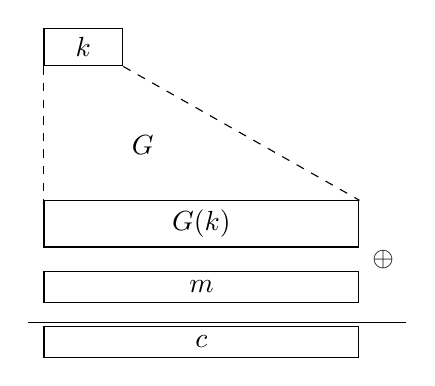
\begin{tikzpicture}
		\node[draw=black, minimum width=1cm] (k) at (0,0){$k$};
		\node[draw=black, minimum width=4cm, anchor=west, shift={(0,-2)}] (Gk) at (k.south west){$G(k)$};
		\node[shift={(1,-1)}, anchor=west] (G) at (k.south west) {$G$};
		\node[draw=black, minimum width=4cm, shift={(0,-0.5)}, anchor=west] (m) at (Gk.south west) {$m$};
		\node[shift={(0.3,-0.15)}] (plus) at (Gk.south east) {$\oplus$};
		\node[draw=black, minimum width=4cm, shift={(0,-0.5)}, anchor=west] (c) at (m.south west) {$c$};
		
		\draw[dashed] (k.south west)--(Gk.north west);
		\draw[dashed] (k.south east)--(Gk.north east);
		\draw (-.7,-3.5)--++(4.8,0);
	\end{tikzpicture}
\end{center}
The function $G$ expands the key space in a way it also looks random. So, we have: $$c=E(k,m):=m\oplus G(k)$$ and $$D(k,c):=c\oplus G(k)$$ But, is it secure?

If a cipher has perfect secrecy the key length must be greater or equal to the message length. So \underline{a stream cipher cannot have perfect secrecy}. Here, we have to use a different definition of security and this property will depend on specific PRG.

\subsubsection{PRG must be unpredictable}
Suppose PRG is predictable, i.e.: $$\exists i:\ G(k)/_{1,\cdots,i}\ \stackrel{alg.}{\longrightarrow}\ G(k)/_{i+1,\cdots,n}$$ where $/_{1,\cdots,i}$ are the first $i$ bits. It says that if we have first $i$ bits of the output of a predictable PRG, we can compute the remainder of the bits. If this happens, the stream cipher is not secure.

Example:
\begin{center}
	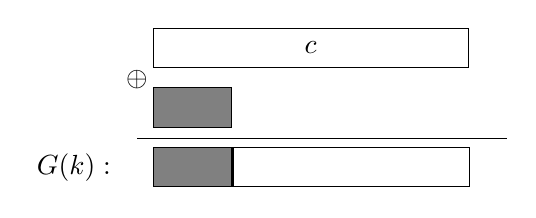
\begin{tikzpicture}
		\node[rectangle, draw=black, minimum width=4cm, minimum height=0.5cm] (c) at (0,0) {$c$};
		\node[rectangle,draw=black,fill=black!50, minimum width=1cm, minimum height=0.5cm,anchor=west,shift={(0,-0.5)}] (know) at (c.south west) {};
		\node[rectangle,draw=black,fill=black!50, minimum width=1cm, minimum height=0.5cm,anchor=west,shift={(0,-0.5)}] (Gknow) at (know.south west) {};
		\node[rectangle,draw=black, minimum width=3cm, minimum height=0.5cm,anchor=west] (G) at (Gknow.east) {};
		
		\node[shift={(-1,0)}] (Gk) at(Gknow.west) {$G(k):$};
		\draw (-2.2,-1.15) --++ (4.7,0);
		\node[shift={(-0.2,-0.15)}] (plus) at (c.south west) {$\oplus$};
	\end{tikzpicture}
\end{center}where \tikz{\node[rectangle,draw=black,fill=black!50, minimum width=1cm, minimum height=0.5cm,anchor=west,shift={(0,-0.5)}] (know) at (0,0) {};}\ is a known part of the plain text (in emails, this known part is ``from:''). So, if we know a part of plain text, we can compute a part of $G(k)$ and, if PRG is predictable, we can compute all $G(k)$, and later we can predict the rest of the plain text.

A small prefix can reveal the entire message if the PRG is predictable and there are secure problems.

Even $\exists i:\ G(k)/_{1,\cdots,i}\ \stackrel{alg.}{\longrightarrow}\ G(k)/_{i+1}$ is a problem.

\Def We say that $G:\mathcal{K}\longrightarrow \{0,1\}^{n}$ is predictable if $$\exists\ \text{``efficient'' algorithm } \mathcal{A}\ and\ \exists\ 1\leq i\leq n-1\ s.t.$$ $$ \underset{k\xleftarrow{R}\mathcal{K}}{Pr}[\mathcal{A}(G(k)/_{1,\cdots,i})=G(k)/_{i+1}]\geq \frac{1}{2}+\varepsilon$$ for some non-negligible $\varepsilon$. (A non-negligible is $\varepsilon\geq\frac{1}{2^{30}}$)

\Def A PRG is unpredictable if it is not predictable $$\Rightarrow\forall i:\ \text{no ``efficient'' adversary can predict bit }(i+1)\text{ for ``non-negligible'' }\varepsilon$$

Example: Suppose $G:\mathcal{K}\longrightarrow\{0,1\}^{n}$ is such that for all $k$: $XOR(G(k))=1$.\\So, we can say that $G$ is predictable, because given the first $(n-1)$ bits, we can predict the $n$'th bit.

A generator must be unpredictable to be secure.

\subsubsection{Weak PRGs (do not use for crypto)}
\textbf{Linear Congruential Generator}: it has three parameters $a,b,p$, where $a,b$ are just integers and $p$ is a prime. It works like below:

\begin{verbatim}
	r[0] = seed
	while not end {
		r[i] = (a * r[i-1] + b) mod p;
		output few bits of r[i];
		i++;
	}
\end{verbatim}It is a very easy algorithm to predict.

\textbf{glibc random()}:
\begin{verbatim}
	glibc random(){
		r[i] = (r[i-3] + r[i-31]) mod 2^32;
		output r[i] >> 1;
	}
\end{verbatim}
We never should use this function for cryptography.

\subsubsection{Negligible and non-negligible}
In \underline{practice}: $\varepsilon$ is a scalar and
\begin{itemize}
	\item $\varepsilon$ non-neg: $\varepsilon\geq\frac{1}{2^{30}}$ (likely to happen over 1GB of data, because 1GB is $2^{30}$ bytes)
	\item $\varepsilon$ neg: $\varepsilon\leq\frac{1}{2^{80}}$ (won't happen over life of key)
\end{itemize}

In \underline{theory}: $\varepsilon$ is a function $\varepsilon:Z^{\geq 0}\longrightarrow R^{\geq 0}$ and
\begin{itemize}
	\item $\varepsilon$ non-neg: $\exists d:\ \varepsilon(\lambda)\geq \frac{1}{\lambda^{d}}$ infinitely often ($\varepsilon\geq\frac{1}{poly}$, for many $\lambda$)
	\item $\varepsilon$ neg: $\forall d,\lambda\geq\lambda_{d}:\ \varepsilon(\lambda)\leq \frac{1}{\lambda^{d}}$ ($\varepsilon\leq\frac{1}{poly}$, for large $\lambda$)
\end{itemize}

Examples:
\begin{itemize}
	\item $\varepsilon(\lambda)=\frac{1}{2^{\lambda}}$: negligible, because there is a large $\lambda$ that this function is less than $\frac{1}{\lambda^{d}}$ and is less than all polynomials.
	\item $\varepsilon(\lambda)=\frac{1}{\lambda^{1000}}$: non-negligible, because if a set $d=10000$, so, clearly, this function is bigger than $\frac{1}{\lambda^{10000}}$.
	\item $\varepsilon=\left\{\begin{array}{ll}
		\frac{1}{2^{\lambda}}&for\ odd\ \lambda\\
		\frac{1}{\lambda^{1000}}&for\ even\ \lambda
	\end{array}\right.$: non-negligible, because $\frac{1}{\lambda^{1000}}$ is very often bigger than $\frac{1}{\lambda^{10000}}$.
\end{itemize}

These terms, basically corresponds to less than polynomial or more than polynomial. In this course, we will use negligible as less than an exponential $\left(e.g.\ \frac{1}{2^{\lambda}}\right)$ and non-negligible as less then one over polynomial $\left(e.g.\ \frac{1}{\lambda^{d}}\right)$.

\newpage
\section{Stream Ciphers 2: attacks and common mistakes}
\subsection{Attacks on Stream Ciphers and The One Time Pad}
\subsubsection{Attack 1: Two time pad is insecure}
We should never use stream cipher key more than once. The one time pad is called like that because the key must be used just once.

Suppose that we use the same key twice:
$$\begin{array}{rcl}
	C_{1}&\leftarrow&m_{1}\oplus PRG(k)\\
	C_{2}&\leftarrow&m_{2}\oplus PRG(k)
\end{array}$$
If an attack gets $C_{1}$ and $C_{2}$ and makes an XOR in it:
$$C_{1}\oplus C_{2}\ \rightarrow\ m_{1}\oplus m_{2}$$
But the combination of \underline{English and ASCII encoding have enough redundancy}, such that given the XOR of two messages, it's possible to recover the messages:
$$m_{1}\oplus m_{2}\ \rightarrow\ m_{1},m_{2}$$

\subsubsection{Real world examples}
\begin{itemize}
	\item Project Venona (1941--1946): using of dices to create pads used to lots of messages.
	\item MS-PPTP\footnote{PPTP: Point-to-point Transfer Protocol} (windows NT):
	\begin{itemize}
		\item It's a protocol for a client wishing to communicate securely with a server, where both share a secret key.
		\item The entire interaction of the client with the server is considered as one stream and is encrypted using a stream cipher using key $k$: $$[m_{1}||m_{2}||\cdots]\oplus PRG(k)\footnote{$||$ means concatenation.}$$
		\item But the same happens with the responses of the server to the client:
		$$[s_{1}||s_{2}||\cdots]\oplus PRG(k)$$ 
		\item The same pad is used twice: not secure. To enhance security, we have to use different keys for Client-to-Server and Server-to-Client interactions. So:
		$$k=\left(k_{s\rightarrow c},k_{c\rightarrow s}\right)$$
		And both sides have this pair of keys.
	\end{itemize}
	\item 802.11b WEP (Wi-Fi communication):
	\begin{center}
		\includegraphics[width=.9\textwidth]{wep}
	\end{center}
	\begin{itemize}
		\item Where $m$ is the message, $CRC(m)$ is a checksum that is appended to the message.
		\item This concatenated text is encrypted (with $\oplus$) using a stream cipher, where the key is the concatenation of the key $k$ (104 bits) and a long value $IV$. So, this concatenated key is changing every frame.
		\item $IV$ is a 24 bits string and works like a counter starting from zero. The value of $IV$ repeats every $2^{24}\approx$16M frames.
		\item The result of the XOR is concatenated to the $IV$ value and sent to the receiver, who knows the key $k$ and the value $IV$ and can recover the message $m$.
		\item The problem is that after 16M messages, the same $IV$ is used to encrypt different messages: two time pad, not secure.
		\item Another problem: on some 802.11 cards, $IV$ resets to 0 after power cycle.
	\end{itemize}
\end{itemize}
\subsubsection{Avoid related keys}
\begin{itemize}
	\item 802.11b WEP:
	\begin{center}
		\includegraphics[width=.9\textwidth]{wep}
	\end{center}
	$$\begin{array}{cc}
		\text{key for frame \#1:}&(1||k)\\
		\text{key for frame \#2:}&(2||k)\\
		\vdots&
	\end{array}$$
	\begin{itemize}
		\item The keys are related to one another. And the PRG used in WEP is not designed to be secure when using related keys that are so closely related. In other words, the majority of these keys are basically the same.
		\item For the PRG used in WEP (RC4), there is an attack discovered by Fluhrer, Mantin and Shamir in 2001. It shows that after about a million frames it's possible to recover the secret key $k$.
		\item Today, there are another attacks and it's sufficient about 40000 frames to recover the key $k$.
	\end{itemize}
\end{itemize}
When we have related keys, security fails.

\subsubsection{A better construction}
The idea is use different parts of the PRG output to different messages.
\begin{center}
	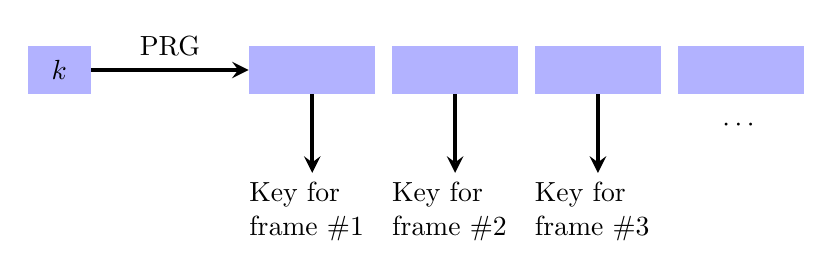
\begin{tikzpicture}
		\node[fill=blue!30, minimum width=0.8cm, minimum height=0.6cm] (k) at (0,0) {$k$};
		\node[shift={(1,0.3)}] (PRG) at (k.east) {PRG};
		\node[fill=blue!30, minimum width=1.6cm, minimum height=0.6cm,anchor=west,shift={(2,0)}] (p1) at (k.east) {};
		\node[fill=blue!30, minimum width=1.6cm, minimum height=0.6cm,anchor=west,shift={(0.2,0)}] (p2) at (p1.east) {};
		\node[fill=blue!30, minimum width=1.6cm, minimum height=0.6cm,anchor=west,shift={(0.2,0)}] (p3) at (p2.east) {};
		\node[fill=blue!30, minimum width=1.6cm, minimum height=0.6cm,anchor=west,shift={(0.2,0)}] (p4) at (p3.east) {};
		
		\node[text width=1.6cm,anchor=north,shift={(0,-1)}] (k1) at (p1.south) {Key for frame \#1};
		\node[text width=1.6cm,anchor=north,shift={(0,-1)}] (k2) at (p2.south) {Key for frame \#2};
		\node[text width=1.6cm,anchor=north,shift={(0,-1)}] (k3) at (p3.south) {Key for frame \#3};
		\node[minimum width=1.6cm,anchor=north,shift={(0,-0.2)}] (k4) at (p4.south) {$\cdots$};
		
		\draw[-stealth, ultra thick] (k.east)--(p1.west);
		
		\draw[-stealth,ultra thick] (p1.south)--(k1.north);
		\draw[-stealth,ultra thick] (p2.south)--(k2.north);
		\draw[-stealth,ultra thick] (p3.south)--(k3.north);
	\end{tikzpicture}
\end{center}
Now, each frame has a pseudorandom key, because every part of the PRG output looks independent of one another.

\subsubsection{Another example: disk encryption}
Suppose a text file begins with \verb|To: Bob|. This file is stored in different blocks in disk. But it's stored encrypted.
\begin{center}
	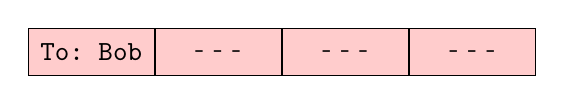
\begin{tikzpicture}
		\node[fill=red!20,draw=black,minimum width=1.6cm,minimum height=0.6cm] (1) at (0,0) {\verb|To: Bob|};
		\node[fill=red!20,draw=black,minimum width=1.6cm,minimum height=0.6cm,anchor=west] (2) at (1.east) {- - -};
		\node[fill=red!20,draw=black,minimum width=1.6cm,minimum height=0.6cm,anchor=west] (3) at (2.east) {- - -};
		\node[fill=red!20,draw=black,minimum width=1.6cm,minimum height=0.6cm,anchor=west] (4) at (3.east) {- - -};
	\end{tikzpicture}
\end{center}The color red means encrypted message.

Now suppose we make just one change in the text \verb|To: Bob| $\rightarrow$ \verb|To: Eve|.
\begin{center}
	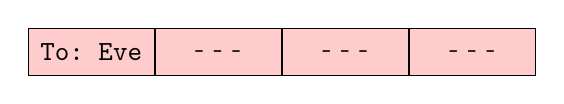
\begin{tikzpicture}
		\node[fill=red!20,draw=black,minimum width=1.6cm,minimum height=0.6cm] (1) at (0,0) {\verb|To: Eve|};
		\node[fill=red!20,draw=black,minimum width=1.6cm,minimum height=0.6cm,anchor=west] (2) at (1.east) {- - -};
		\node[fill=red!20,draw=black,minimum width=1.6cm,minimum height=0.6cm,anchor=west] (3) at (2.east) {- - -};
		\node[fill=red!20,draw=black,minimum width=1.6cm,minimum height=0.6cm,anchor=west] (4) at (3.east) {- - -};
	\end{tikzpicture}
\end{center}
The attacker realizes that just one segment of the encrypted text is different: the segment where the change (Bob to Eve) was made. So he can tell where a change was made, even he doesn't know what changed.

This is another example of two time pad application, because the same pad is used to encrypt different texts.

\subsubsection{Two time pad: summary}
Never use stream cipher key more than once!
\begin{itemize}
	\item Network traffic: negotiate new key for every session (e.g. TLS)
	\item Disk encryption: typically do no use a stream cipher
\end{itemize}

\subsubsection{Attack 2: no integrity (OTP is malleable)}
The one time pad and stream ciphers in general provide no integrity at all. They try to provide confidentiality, but no integrity. And it's very easy to modify cipher text and have known effects on the corresponding plain text. This property is called malleability.

Suppose we have a encryption like:
\begin{center}
	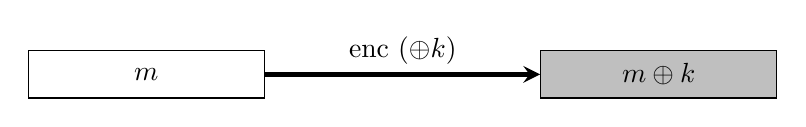
\begin{tikzpicture}
		\node[minimum width=3cm,minimum height=0.6cm,draw=black] (m) at (0,0) {$m$};
		\node[shift={(1.75,0.3)}] (enc) at (m.east) {enc $(\oplus k)$};
		\node[minimum width=3cm,minimum height=0.6cm,draw=black, fill=gray!50,shift={(5,0)}] (mk) at (m.east) {$m\oplus k$};
		
		\draw[-stealth,ultra thick] (m.east)--(mk.west);
	\end{tikzpicture}
\end{center}
The attacker can modify the cipher text by XOR the cipher text with a value $p$ (also called by perturbation $p$):
\begin{center}
	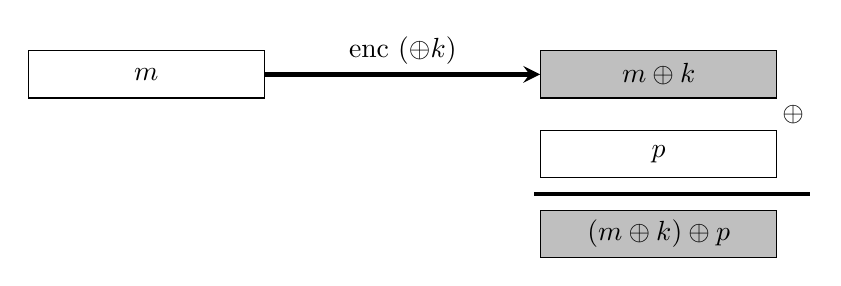
\begin{tikzpicture}
		\node[minimum width=3cm,minimum height=0.6cm,draw=black] (m) at (0,0) {$m$};
		\node[shift={(1.75,0.3)}] (enc) at (m.east) {enc $(\oplus k)$};
		\node[minimum width=3cm,minimum height=0.6cm,draw=black, fill=gray!50,shift={(5,0)}] (mk) at (m.east) {$m\oplus k$};
		\node[minimum width=3cm,minimum height=0.6cm,draw=black,shift={(0,-0.4)},anchor=north] (p) at (mk.south) {$p$};
		\node[shift={(0.2,-0.2)}] (plus) at (mk.south east) {$\oplus$};
		\node[minimum width=3cm,minimum height=0.6cm,draw=black,fill=gray!50,shift={(0,-0.4)},anchor=north] (mkp) at (p.south) {$(m\oplus k)\oplus p$};
		
		\draw[-stealth,ultra thick] (m.east)--(mk.west);
		\node[shift={(-0.2,-0.2)}] (space) at (p.south west){};
		\draw[ultra thick] (space.east)--++(3.5,0);
	\end{tikzpicture}
\end{center}
With this modification, the decrypted message will be:
\begin{center}
	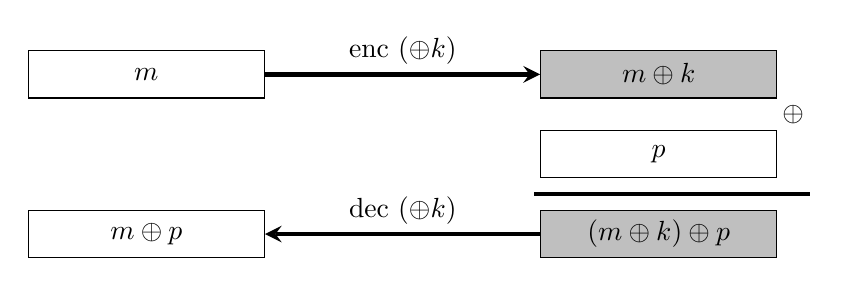
\begin{tikzpicture}
		\node[minimum width=3cm,minimum height=0.6cm,draw=black] (m) at (0,0) {$m$};
		\node[shift={(1.75,0.3)}] (enc) at (m.east) {enc $(\oplus k)$};
		\node[minimum width=3cm,minimum height=0.6cm,draw=black, fill=gray!50,shift={(5,0)}] (mk) at (m.east) {$m\oplus k$};
		\node[minimum width=3cm,minimum height=0.6cm,draw=black,shift={(0,-0.4)},anchor=north] (p) at (mk.south) {$p$};
		\node[shift={(0.2,-0.2)}] (plus) at (mk.south east) {$\oplus$};
		\node[minimum width=3cm,minimum height=0.6cm,draw=black,fill=gray!50,shift={(0,-0.4)},anchor=north] (mkp) at (p.south) {$(m\oplus k)\oplus p$};
		\node[minimum width=3cm,minimum height=0.6cm,draw=black,shift={(-5,0)}] (mp) at (mkp.west) {$m\oplus p$};
		\node[shift={(1.75,0.3)}] (dec) at (mp.east) {dec $(\oplus k)$};
		
		\draw[-stealth,ultra thick] (m.east)--(mk.west);
		\node[shift={(-0.2,-0.2)}] (space) at (p.south west){};
		\draw[ultra thick] (space.east)--++(3.5,0);
		\draw[-stealth,ultra thick] (mkp.west)--(mp.east);
	\end{tikzpicture}
\end{center}What we see is, even we using XOR at the cipher text, we obtained the same that using XOR at the plain text recovered.

Modifications to cipher text are undetected and have \underline{predictable} impact on plain text.

Example: Suppose that the attacker knows that the message is \verb|From: Bob|, so he can modify the recovered message.
\begin{center}
	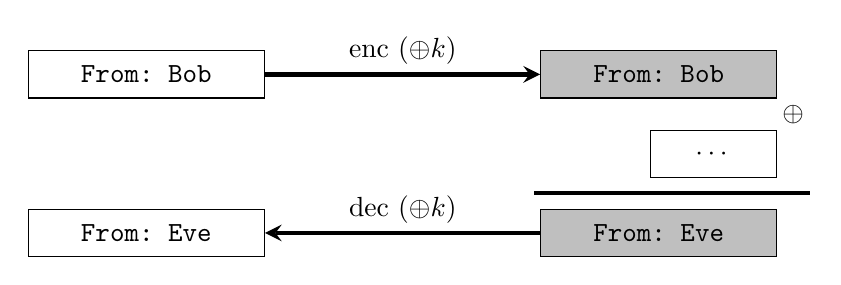
\begin{tikzpicture}
		\node[minimum width=3cm,minimum height=0.6cm,draw=black] (m) at (0,0) {\verb|From: Bob|};
		\node[shift={(1.75,0.3)}] (enc) at (m.east) {enc $(\oplus k)$};
		\node[minimum width=3cm,minimum height=0.6cm,draw=black, fill=gray!50,shift={(5,0)}] (mk) at (m.east) {\verb|From: Bob|};
		\node[minimum width=1.6cm,minimum height=0.6cm,draw=black,shift={(0,-0.4)},anchor=north east] (p) at (mk.south east) {$\cdots$};
		\node[shift={(0.2,-0.2)}] (plus) at (mk.south east) {$\oplus$};
		\node[minimum width=3cm,minimum height=0.6cm,draw=black,fill=gray!50,shift={(0,-1.4)},anchor=north] (mkp) at (mk.south) {\verb|From: Eve|};
		\node[minimum width=3cm,minimum height=0.6cm,draw=black,shift={(-5,0)}] (mp) at (mkp.west) {\verb|From: Eve|};
		\node[shift={(1.75,0.3)}] (dec) at (mp.east) {dec $(\oplus k)$};
		
		\draw[-stealth,ultra thick] (m.east)--(mk.west);
		\node[shift={(-0.2,-1.2)}] (space) at (mk.south west){};
		\draw[ultra thick] (space.east)--++(3.5,0);
		\draw[-stealth,ultra thick] (mkp.west)--(mp.east);
	\end{tikzpicture}
\end{center}
Using XOR between the words Bob and Eve we can know what characters the attacker must use to change the message.
\begin{center}
	\begin{tabular}{|c|ccc|ccc|ccc|}
		\hline
		Message&B&o&b&E&v&e&\multicolumn{3}{c|}{Bob $\oplus$ Eve *}\\\hline
		ASCII to Hex&42&6F&62&45&76&65&07&19&07\\\hline
	\end{tabular}
	\\[0.1cm]* The XOR between the words is made letter by letter.
\end{center}So we have:
\begin{center}
	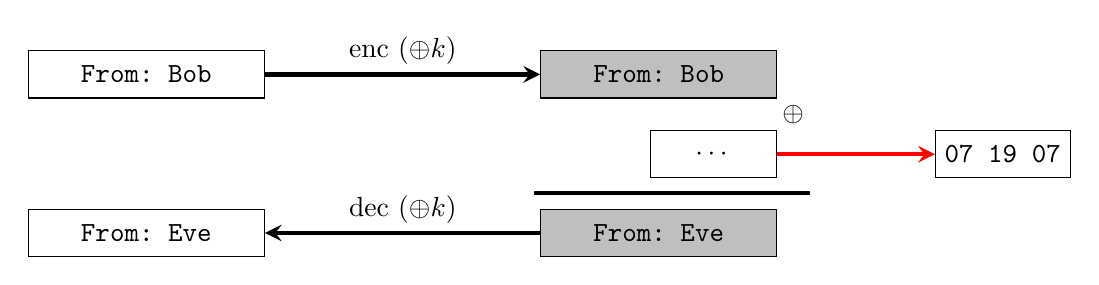
\begin{tikzpicture}
		\node[minimum width=3cm,minimum height=0.6cm,draw=black] (m) at (0,0) {\verb|From: Bob|};
		\node[shift={(1.75,0.3)}] (enc) at (m.east) {enc $(\oplus k)$};
		\node[minimum width=3cm,minimum height=0.6cm,draw=black, fill=gray!50,shift={(5,0)}] (mk) at (m.east) {\verb|From: Bob|};
		\node[minimum width=1.6cm,minimum height=0.6cm,draw=black,shift={(0,-0.4)},anchor=north east] (p) at (mk.south east) {$\cdots$};
		\node[shift={(0.2,-0.2)}] (plus) at (mk.south east) {$\oplus$};
		\node[minimum width=3cm,minimum height=0.6cm,draw=black,fill=gray!50,shift={(0,-1.4)},anchor=north] (mkp) at (mk.south) {\verb|From: Eve|};
		\node[minimum width=3cm,minimum height=0.6cm,draw=black,shift={(-5,0)}] (mp) at (mkp.west) {\verb|From: Eve|};
		\node[shift={(1.75,0.3)}] (dec) at (mp.east) {dec $(\oplus k)$};
		\node[minimum width=1.6cm,minimum height=0.6cm,draw=black,shift={(2,0)},anchor=west] (pm) at (p.east) {\verb|07 19 07|};
		
		\draw[-stealth,ultra thick] (m.east)--(mk.west);
		\node[shift={(-0.2,-1.2)}] (space) at (mk.south west){};
		\draw[ultra thick] (space.east)--++(3.5,0);
		\draw[-stealth,ultra thick] (mkp.west)--(mp.east);
		\draw[-stealth,ultra thick,draw=red] (p.east)--(pm.west);
	\end{tikzpicture}
\end{center}Only what the attacker knows is part of the plain text. And he can modify the recovered text without knowing the cipher text.

This is an example where having a predictable impact on the cipher text can actually cause a bit of problems. And this property is called malleability.

The one time pad is malleable because it's very easy to compute in cipher texts and make prescribed changes to the corresponding plain texts.

Later we will see how to add integrity to encryption mechanisms in general.

\newpage
\section{Stream Cipher 3: real-world examples}
\subsection{Real-World Stream Ciphers}
\subsubsection{Old example (software): RC4 (1987)}
\begin{center}
	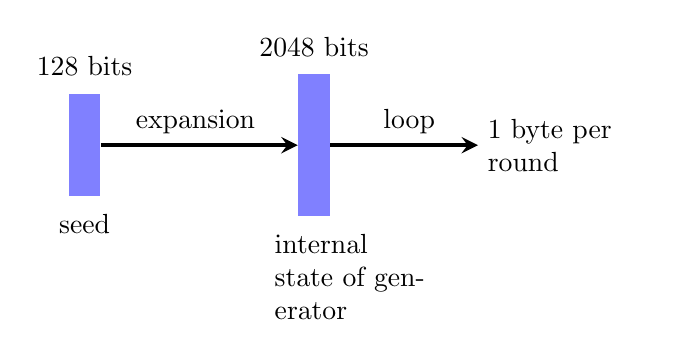
\begin{tikzpicture}
		\node[minimum height=1.3cm, minimum width=0.4cm, fill=blue!50] (seed) {};
		\node[below=0.1cm of seed] (seedt) {seed};
		\node[above=0.1cm of seed] (128b) {128 bits};
		
		\node[minimum height=1.8cm, minimum width=0.4cm, fill=blue!50, right=2.5cm of seed] (seedexp) {};
		\node[below=0.1cm of seedexp, text width = 2cm,anchor=north,shift={(0.5,0)}] (seedexpt) {internal state of generator};
		\node[above=0.1cm of seedexp] (2048b) {2048 bits};
		
		\node[text width=2cm,shift={(3,0)}] (out) at (seedexp.east){1 byte per round};
		
		\draw[-stealth, ultra thick] (seed)--(seedexp);
		\draw[-stealth, ultra thick] (seedexp)--(out);
		\node[shift={(1,0.3)}] (loop) at (seedexp.east) {loop};
		\node[shift={(1.2,0.3)}] (exp) at (seed.east) {expansion};
	\end{tikzpicture}
\end{center}Where seed is the secret key, that is expanded to a larger key, that's used as internal state of the generator.
\begin{itemize}
	\item Used in HTTPS and WEP
	\item Weaknesses:
	\begin{itemize}
		\item Bias in initial output: $Pr[2^{nd}\ byte=0]=\frac{2}{256}$. It should be $\frac{1}{256}$, if it was completely random. Suggestion: ignore the first 256 bytes, because of bias.
		\item Prob. of $(0,0)$ is $\frac{1}{256^{2}}+\frac{1}{256^{3}}$. It should be $\frac{1}{256^{2}}$, if it was completely random. (This bias stars after gigabytes of data)
		\item Related key attacks.
	\end{itemize}
\end{itemize}
Its recommended not to use RC4 in new systems.

\subsubsection{Old example (hardware): CSS -- Content Scrambling System (badly broken)}
Used to encrypted DVD movies.

Linear feedback shift register (LSFR):
\begin{center}
	\begin{tikzpicture}
		\node[draw=black, minimum width=1.5cm, minimum height=0.6cm] (s1) {};
		\node[draw=black, minimum width=1.5cm, minimum height=0.6cm,anchor=west] (s2) at (s1.east) {};
		\node[draw=black, minimum width=1.5cm, minimum height=0.6cm,anchor=west] (s3) at (s2.east) {};
		\node[draw=black, minimum width=1.5cm, minimum height=0.6cm,anchor=west] (s4) at (s3.east) {};
		\node[draw=black, minimum width=1.5cm, minimum height=0.6cm,anchor=west] (s5) at (s4.east) {};
		\node[draw=black, minimum width=1.5cm, minimum height=0.6cm,anchor=west] (s6) at (s5.east) {};
		\node[draw=black, minimum width=1.5cm, minimum height=0.6cm,anchor=west] (s7) at (s6.east) {};
		\node[draw=black, minimum width=1.5cm, minimum height=0.6cm,anchor=west] (s8) at (s7.east) {};
		\node[draw=black, minimum width=1.5cm, minimum height=0.6cm,anchor=west] (s9) at (s8.east) {};
		
		\node[shift={(0,-2)}] (plus) at (s5.south) {{\large $\mathbf{\oplus}$}};
		\draw[dashed,draw opacity=0.7] (s2.south)--(plus.center);
		\draw[dashed,draw opacity=0.7] (s4.south)--(plus.center);
		\draw[dashed,draw opacity=0.7] (s8.south)--(plus.center);
		
		\draw[-stealth,ultra thick] (3,0.75)--++(6.5,0);
		\draw[-stealth,dashed,draw opacity=0.7] (plus.center)-|(s1.south);
		\node[shift={(0,-2)}] (plus1) at (s5.south) {{\large $\mathbf{\oplus}$}};
		\draw[-stealth,ultra thick] (s9.east)--++(1,0);
	\end{tikzpicture}
\end{center}
The seed is the initial state of the LFSR.

CSS: seed = 5 bytes = 40 bits (legally limited).
\begin{center}
	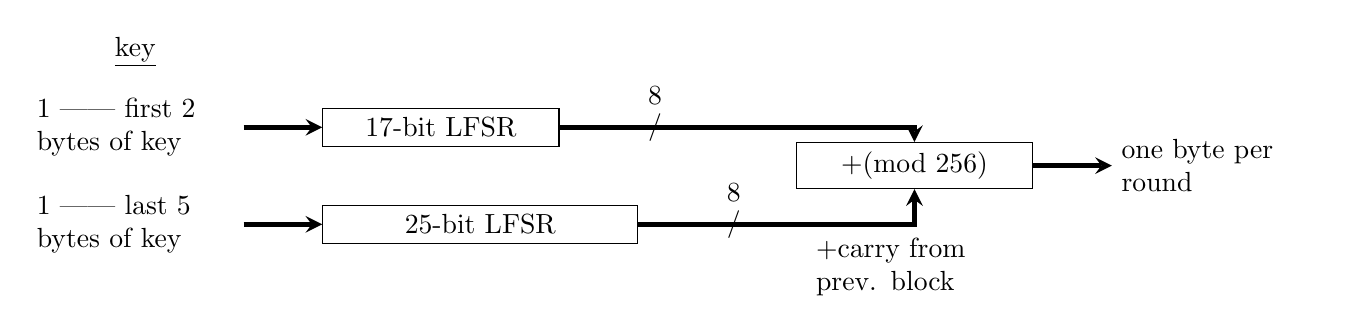
\begin{tikzpicture}
		\node (key) {\underline{key}};
		\node[below=0.15cm of key,text width=2.5cm] (keyf) {1 || first 2 bytes of key};
		\node[below=0.25cm of keyf,text width=2.5cm] (keyl) {1 || last 5 bytes of key};
		\node[draw=black,right=of keyf, minimum width=3cm] (lfsr1) {17-bit LFSR};
		\node[draw=black,right=of keyl, minimum width=4cm] (lfsr2) {25-bit LFSR};
		\node[draw=black, shift={(2,0.5)}, minimum width=3cm,anchor=west] (mod) at (lfsr2.north east) {+(mod 256)};
		\node[below=0.5cm of mod, text width=2.5cm] (carry) {+carry from prev. block};
		\node[right=of mod, text width=2.5cm] (out) {one byte per round};
		\node[right=of lfsr2] (sl2) {/};
		\node[right=of lfsr1] (sl1) {/};
		\node[shift={(0,0.1)}] (82) at (sl2.north) {8};
		\node[shift={(0,0.1)}] (81) at (sl1.north) {8};
		
		\draw[-stealth, ultra thick] (keyf.east)--(lfsr1.west);
		\draw[-stealth, ultra thick] (keyl.east)--(lfsr2.west);
		\draw[-stealth, ultra thick] (lfsr2.east)-|(mod.south);
		\draw[-stealth, ultra thick] (lfsr1.east)-|(mod.north);
		\draw[-stealth, ultra thick] (mod.east)--(out.west);
	\end{tikzpicture}
\end{center}It's easy to break in time roughly $2^{17}$. That happens because the DVD movies are stored using a MPEG file. Because of this, we know a prefix of the plain text.

Suppose we know the first 20 bytes of MPEG file, so we can recover the first 20 bytes of PRG, by using XOR. So we try all the $2^{17}$ possible values of the first LFSR and for every value of this as initial state we run the LFSR for 20 bytes. Later, we subtract the 20 bytes obtained from the 20 bytes known of the PRG and, if the initial state of first LFSR is correct, we obtain the first 20 bytes output of second LFSR. It turns out that is easy to figure out if a 20 bytes output came from a 25-bit LFSR. If didn't, our guess for initial state of 17-bit LFSR is incorrect. And we keep trying until find the correct one and obtain both initial states. After this, we have the secret key and it's possible to decrypt all the DVD movie.

Other weak examples:
$$\left.\begin{array}{l}
	\text{DVD encryption (CSS): 2 LFSRs}\\[0.2cm]
	\text{GSM encryption (A5/1,2): 3 LFSRs}\\[0.2cm]
	\text{Bluetooth (E0): 4 LFSRs}\\
\end{array}\ \ \ \right\}\ \text{all broken}$$

\subsubsection{Modern stream ciphers: eStream}
Better PRGs come from the eStream Project, concluded in 2008. They present 5 different stream ciphers, but we will see only one here.
$$PRG:\ \{0,1\}^{s}\times R\ \rightarrow\ \{0,1\}^{n},\ \ \ n>>s$$where $\{0,1\}^{s}$ is the seed and $R$ is the nonce.

\Def Nonce is a non-repeating value for a given key.

The encryption is given as follows:
$$E(k,m;r)=m\oplus PRG(k;r)$$where the pair $(k,r)$ is never used more than once. So we can re-use the key because the pair $(k,r)$ is unique.

\subsubsection{eStream: Salsa20 (Software + Hardware)}
It's easy to implement in hardware and its software implementation runs very fast.
$$Salsa20:\ \{0,1\}^{128\ or\ 256}\times\{0,1\}^{64}\ \rightarrow\ \{0,1\}^{n},\ \ \ (\max n=2^{73}\ bits)$$where $\{0,1\}^{128\ or\ 256}$ is the seed and $\{0,1\}^{64}$ is the nonce.

\Def Salsa20 is defined as follows:
$$Salsa20(k;r):=H\big(k,(r,0)\big)\ ||\ H\big(k,(r,1)\big)\ ||\ \cdots$$where $H$ is a function with three inputs: the key $k$, the nonce $r$ and an incrementing counter starting from zero.

The function H works as follows: firstly, it expands the states into something large (64 bytes long).
\begin{center}
	\resizebox{\textwidth}{!}{%
		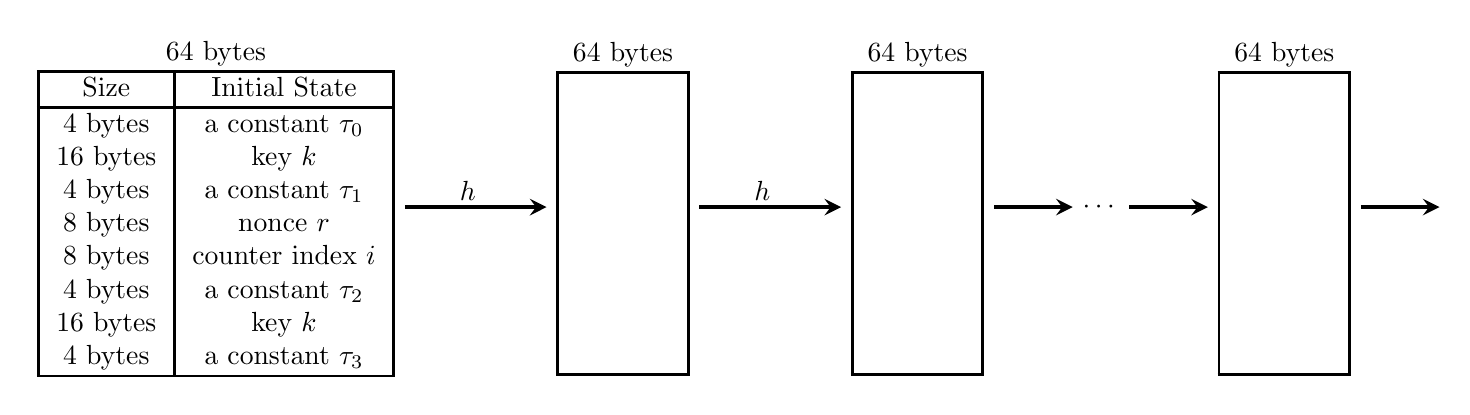
\begin{tikzpicture}
			\node (ini) {%
				\begin{tabular}{|c|c|}
					
					\multicolumn{2}{c}{64 bytes}\\\hline
					Size&Initial State\\\hline
					4 bytes&a constant $\tau_{0}$\\
					16 bytes& key $k$\\
					4 bytes& a constant $\tau_{1}$\\
					8 bytes& nonce $r$\\
					8 bytes& counter index $i$\\
					4 bytes& a constant $\tau_{2}$\\
					16 bytes& key $k$\\
					4 bytes& a constant $\tau_{3}$\\\hline
			\end{tabular}};
			\node[shift={(0.8,0.2)}] (h) at (ini.east) {$h$};
			\node[right=1.8cm of ini] (hout) {%
				\begin{tabular}{|cc|}
					\multicolumn{2}{c}{64 bytes}\\\hline
					& \\
					& \\
					& \\
					& \\
					& \\
					& \\
					& \\
					& \\
					& \\\hline
			\end{tabular}};
			\node[shift={(0.8,0.2)}] (h) at (hout.east) {$h$};
			\node[right=1.8cm of hout] (hout1) {%
				\begin{tabular}{|cc|}
					\multicolumn{2}{c}{64 bytes}\\\hline
					& \\
					& \\
					& \\
					& \\
					& \\
					& \\
					& \\
					& \\
					& \\\hline
			\end{tabular}};
			\node[right=of hout1] (pontos) {$\cdots$};
			\node[right=of pontos] (hout2) {%
				\begin{tabular}{|cc|}
					\multicolumn{2}{c}{64 bytes}\\\hline
					& \\
					& \\
					& \\
					& \\
					& \\
					& \\
					& \\
					& \\
					& \\\hline
			\end{tabular}};
			
			\draw[-stealth, ultra thick] (ini.east)--(hout.west);
			\draw[-stealth, ultra thick] (hout.east)--(hout1.west);
			\draw[-stealth, ultra thick] (hout1.east)--(pontos.west);
			\draw[-stealth, ultra thick] (pontos.east)--(hout2.west);
			\draw[-stealth, ultra thick] (hout2.east)--++(1,0);
		\end{tikzpicture}
	}
\end{center}where $h$ is a invertible function designed to be fast on x86 (SSE2) and is applied 10 times above. But the output of the sketch showed above is not random, because $h$ is invertible and it's easy to recover the initial state given the output. To become a PRG, we take the initial state and sum it, byte-by-byte, with the output of the tenth $h$ output. The result of this sum is the output of the $H$ function.

Basically, there are no significant attacks on this and it has security very close to $2^{128}$. As far as we can tell, it seems to be unpredictable.

\newpage
\section{Stream Ciphers 4: what is a secure cipher?}
\subsection{PRG Security Definitions}
Let $G:\mathcal{K}\rightarrow \{0,1\}^{n}$ be a PRG.

\underline{Goal}: define what it means that
$$\left[k\xleftarrow{R}\mathcal{K},\ output\ G(k)\right]$$is ``indistinguishable'' from
$$\left[r\xleftarrow{R}\{0,1\}^{n},\ output\ r\right]$$
\subsubsection{Statistical Tests}
\Def Statistical test on $\{0,1\}^{n}$:
$$\text{an alg. }A\ s.t.\ A(x)\text{ outputs ``0'' or ``1''}$$where output zero is because input is not random and one is input random.

Examples:
\begin{enumerate}
	\item $A(x)=1,\ iff\ \left|\#0(x)-\#1(x)\right|\leq 10\cdot\sqrt{n}$, where $10\cdot \sqrt{n}$ is a way to say that difference is not so big.\footnote{$iff$: if and only if.}
	\item $A(x)=1,\ iff\ \left|\#00(x)-\frac{n}{4}\right|\leq 10\cdot\sqrt{n}$, where $10\cdot \sqrt{n}$ is a way to say that number of 00 is roughly $\frac{n}{4}$.\footnote{$\#00(x)$: the number of times we see two consecutive zeros.}
	\item $A(x)=1,\ iff\ \text{max-run-of-0}(x)\leq 10\cdot \log_{2}(n)$
\end{enumerate}
We can say that a generator is random if a bunch of statistical tests say so. Using a fixed set of statistical sets is not good for security in crypto.

\subsubsection{Advantage}
Let $G:\mathcal{K}\rightarrow\{0,1\}^{n}$ be a PRG and $A$ a statistical test on $\{0,1\}^{n}$.

\Def 
$$Adv_{PRG}[A,G]:=\left|\underset{k\xleftarrow{R}\mathcal{K}}{Pr[}A(G(k))=1]-\underset{r\xleftarrow{R}\{0,1\}^{n}}{Pr[A(r)}=1]\right|\in[0,1]$$

If the advantage is close to 1: the statistical test $A$ behaves differently for pseudo-random inputs and truly random inputs. In other words, $A$ can distinguish $G$ from random.

If the advantage is close to 1: the statistical test $A$ behaves similarly for pseudo-random inputs and truly random inputs. In other words, $A$ cannot distinguish $G$ from random.

Example: If $A(x)=0$, so we have $Adv_{PRG}[A,G]=0$. $A$ cannot distinguish $G$ from random.

Example: Suppose $G:\mathcal{K}\rightarrow\{0,1\}^{n}$ satisfies $msb(G(k))=1$ for 2/3 of keys in $\mathcal{K}$.\\
Define statistical test $A(x)$ as:
$$if\ [msb(x)=1]\text{ output ``1'' else output ``0''}$$Then:
$$Adv_{PRG}[A,G]=\left|Pr[A(G(k))=1]-Pr[A(r)=1]\right|=\frac{2}{3}-\frac{1}{2}=\frac{1}{6}$$that is a non-negligible number. In other words, $A$ can distinguish the output. $A$ breaks generator $G$ with advantage $\frac{1}{6}$.

\subsubsection{Secure PRGs: crypto definition}
\Def We say that $G:\mathcal{K}\rightarrow\{0,1\}^{n}$ is a secure PRG if no ``efficient'' statistical tests can distinguish its output from random. In other words:
$$\forall \text{ ``efficient'' statistical tests }A:\ Adv_{PRG}[A,G]\text{ is ``negligible''.}$$The statistical test must be efficient. But are there provably secure PRGs? No. At least, it's not known there are provably secure PRGs. but we have a lot of heuristic candidates.

\subsubsection{Easy fact: a secure PRG is unpredictable}
To show this we show the contra-positive:
\begin{center}
	PRG predictable $\Rightarrow$ PRG is insecure.
\end{center}

Suppose $A$ is an efficient algorithm s.t. 
$$\underset{k\xleftarrow{R}\mathcal{K}}{Pr}\left[A\left(G(k)/_{1,\cdots,i}\right)=G(k)/_{i+1}\right]\geq\frac{1}{2}+\varepsilon$$for non-negligible $\varepsilon$ (e.g. $\varepsilon=\frac{1}{1000}$).

Define statistical test $B$ as:
$$B(x)=\left[\begin{array}{cl}
	1,\ if&A\left(x/_{1,\cdots,i}\right) =x/_{i+1}\\[0.2cm]
	0,\ if&A\left(x/_{1,\cdots,i}\right) \neq x/_{i+1}
\end{array}\right.$$

If we have: $r\xleftarrow{R}\{0,1\}^{n}$, so: $Pr[B(r)=1]=\frac{1}{2}$, because it's truly random and the first $i$ bits are independent of the $i+1$ bit.

If we have: $r\xleftarrow{R}\mathcal{K}$, so: $Pr[B(G(k))=1]\geq\frac{1}{2}+\varepsilon$.

Then:
$$Adv_{PRG}[B,G]\geq\varepsilon$$In other words, $G$ is insecure.

The contra-positive is:
\begin{center}
	PRG is secure $\Rightarrow$ PRG unpredictable.
\end{center}

\subsubsection{Theorem (Yao'82): an unpredictable PRG is secure}
Let $G:\mathcal{K}\rightarrow\{0,1\}^{n}$ be a PRG.

\Thm if $\forall i\in\{0,\cdots,n-1\}$ PRG $G$ is unpredictable at position $i$, then $G$ is a secure PRG.

In other words, if next-bit predictors can not distinguish $G$ from random then no statistical test can.

Implication: Let $G:\mathcal{K}\rightarrow\{0,1\}^{n}$ be a PRG such that from the last $\frac{n}{2}$ bits of $G(k)$ it is easy to compute the first $\frac{n}{2}$ bits. So $G$ is predictable for some $i\in\{0,\cdots,n-1\}$, because $G$ is not secure. As we did previously, it's easy to build a statistical test that makes advantage not close to zero. Then, if it is not secure, it's predictable.

\subsubsection{More Generally}
Let $P_{1}$ and $P_{2}$ be two distributions over $\{0,1\}^{n}$.

\Def We say that $P_{1}$ and $P_{2}$ are \textbf{computationally indistinguishable} (denoted $P_{1}\approx_{p}P_{2}$, i.e. in polynomial time, $P_{1}$ ca not be distinguished from $P_{2}$):
$$if\ \forall\ \text{``efficient'' statistical tests }A:\ \left|\underset{x\leftarrow P_{1}}{Pr}[A(x)=1]-\underset{x\leftarrow P_{2}}{Pr}[A(x)=1]\right|<\text{negligible}$$

Example: a PRG is secure if: $\{k\xleftarrow{R}\mathcal{K}:G(k)\}\approx_{p}\ uniform(\{0,1\}^{n})$

\subsection{Semantic Security}
\underline{Goal}: secure PRG $\Rightarrow$ ``secure'' stream cipher.
\subsubsection{What is a secure cipher?}
For now, we know that attacker's abilities is obtain one cipher text..

Possible security requirements:
\begin{enumerate}
	\item[] Attempt \#1: attacker cannot recover secret key.
	\begin{itemize}
		\item If the cipher is $E(k,m)=m$, the attacker has the plain text, because it is the same of cipher text. Bad requirement.
	\end{itemize}
	\item[] Attempt \#2: attacker cannot recover all of plain text.
	\begin{itemize}
		\item If the cipher is $E(k,m_{0}||m_{1})=m_{0}||E(k,m_{1})$, the attacker has part of the plain text. Insecure.
	\end{itemize}
	\item[] Recall Shannon's idea: cipher text should reveal no ``info'' about plain text.
\end{enumerate}

\subsubsection{Recall Shannon's perfect secrecy}

Let $(E,D)$ be a cipher over $(\mathcal{K},\mathcal{M},\mathcal{C})$.

$(E<D)$ has perfect secrecy if $\forall m_{0},m_{1}\in\mathcal{M},\ (|m_{0}|=|m_{1}|)$ then $$\{E(k,m_{0})\}=\{E(k,m_{1})\}\ where\ k\leftarrow\mathcal{K}$$But we see that it depends on size of keys.

For stream ciphers we can modify the definition to:\\
$(E<D)$ has perfect secrecy if $\forall m_{0},m_{1}\in\mathcal{M},\ (|m_{0}|=|m_{1}|)$ then $$\{E(k,m_{0})\}\approx_{p}\{E(k,m_{1})\}\ where\ k\leftarrow\mathcal{K}$$where $\{E(k,m_{0})\}$ denotes the distribution of $E(k,m_{0})$. In other words, the attacker can not distinguish the two distributions or he can't tell what distribution the cipher came from.

But the definition above still is too strong. So we can substitute the $\forall m_{0},m_{1}$ for only pairs $m_{0},m_{1}$ that the attacker could actually exhibit.

\subsubsection{Semantic Security (one-time key: when the attacker is only given one cipher text)}
For $b\in\{0,1\}$ define experiments $EXP(0)$ and $EXP(1)$ as:
\begin{center}
	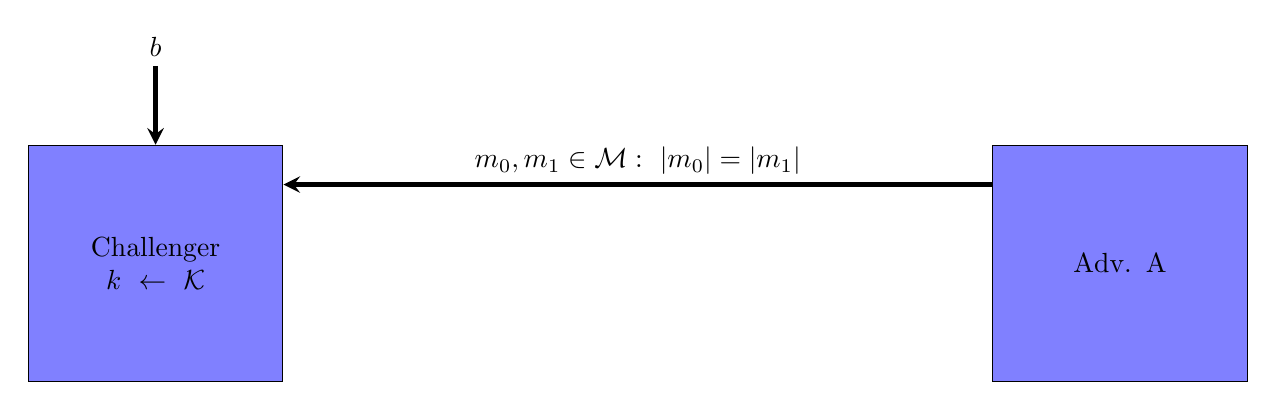
\begin{tikzpicture}
		\node[draw=black,fill=blue!50,minimum size=3cm, text width=3cm,align=center] (chal) {Challenger \ \ $k\leftarrow\mathcal{K}$};
		\node[draw=black,fill=blue!50,minimum size=3cm, text width=3cm,align=center,right=9cm of chal] (adv) {Adv. A};
		\node[shift={(4.5,1.3)}] (ACm) at (chal.east) {$m_{0},m_{1}\in\mathcal{M}:\ |m_{0}|=|m_{1}|$};
		\node[above=of chal] (b) {$b$};
		
		\begin{scope}[transform canvas={yshift=1cm}]
			\draw[-stealth, ultra thick] (adv.west)--(chal.east);
		\end{scope}
		\draw[-stealth,ultra thick] (b.south)--(chal.north);
	\end{tikzpicture}
\end{center}
Firstly, we see above that the adversary outputs the pair of messages the attacker wants to be challenged on.

\begin{center}
	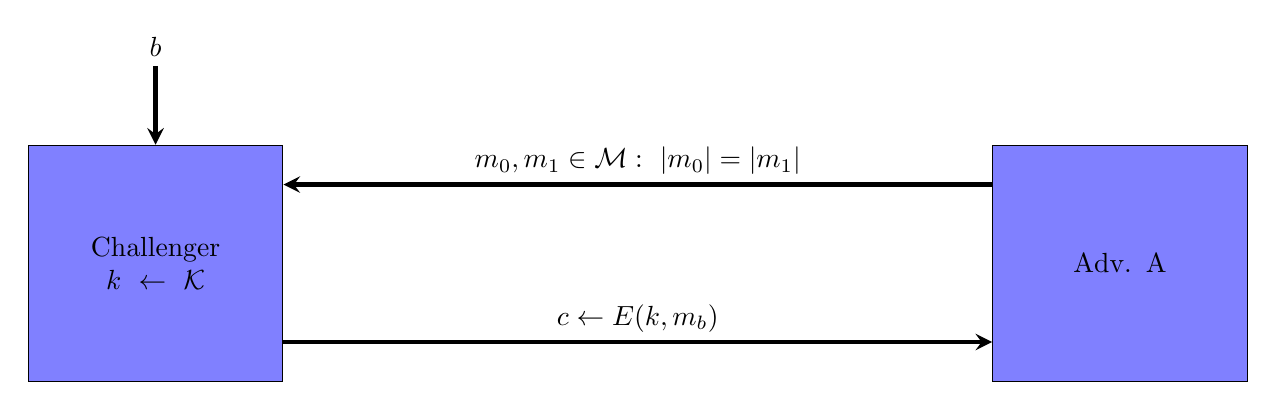
\begin{tikzpicture}
		\node[draw=black,fill=blue!50,minimum size=3cm, text width=3cm,align=center] (chal) {Challenger \ \ $k\leftarrow\mathcal{K}$};
		\node[draw=black,fill=blue!50,minimum size=3cm, text width=3cm,align=center,right=9cm of chal] (adv) {Adv. A};
		\node[shift={(4.5,1.3)}] (ACm) at (chal.east) {$m_{0},m_{1}\in\mathcal{M}:\ |m_{0}|=|m_{1}|$};
		\node[shift={(4.5,-0.7)}] (CAm) at (chal.east) {$c\leftarrow E(k,m_{b})$};
		\node[above=of chal] (b) {$b$};
		
		\begin{scope}[transform canvas={yshift=1cm}]
			\draw[-stealth, ultra thick] (adv.west)--(chal.east);
		\end{scope}
		\begin{scope}[transform canvas={yshift=-1cm}]
			\draw[-stealth, ultra thick] (chal.east)--(adv.west);
		\end{scope}
		\draw[-stealth,ultra thick] (b.south)--(chal.north);
	\end{tikzpicture}
\end{center}
Secondly, we see above that the challenger outputs the encryption of $m_{0}$ in $EXP(0)$ and $m_{1}$ in $EXP(1)$. And, after this, the adversary tries to guess what $b$ was the input of the challenger, as we see below. In other words, it tries to guess whether he was given the encryption of $m_0$ or $m_{1}$.
\begin{center}
	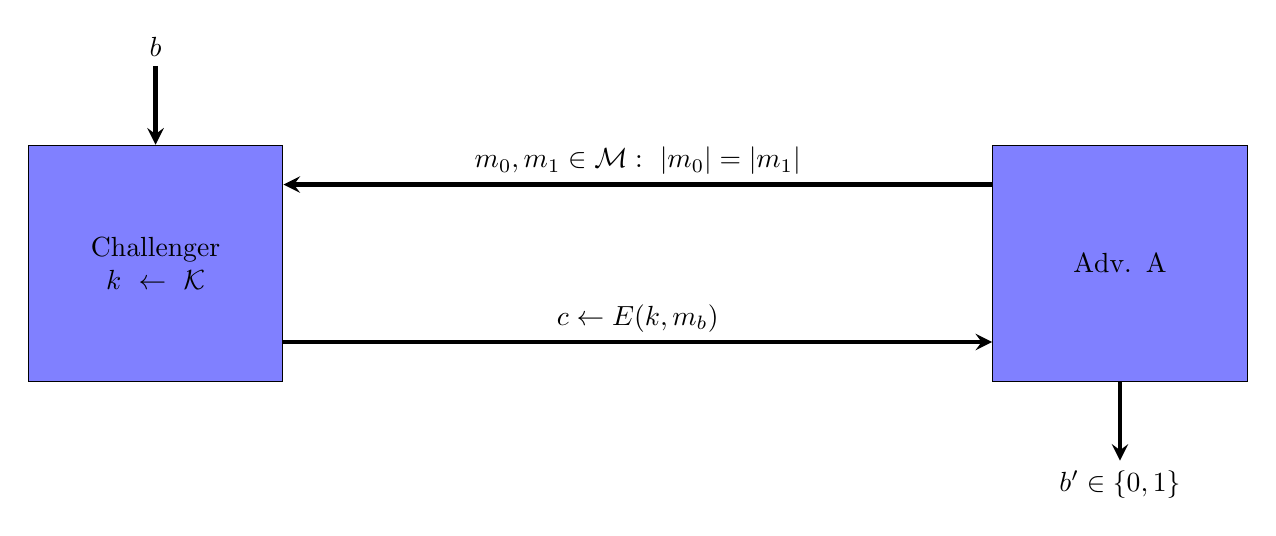
\begin{tikzpicture}
		\node[draw=black,fill=blue!50,minimum size=3cm, text width=3cm,align=center] (chal) {Challenger \ \ $k\leftarrow\mathcal{K}$};
		\node[draw=black,fill=blue!50,minimum size=3cm, text width=3cm,align=center,right=9cm of chal] (adv) {Adv. A};
		\node[shift={(4.5,1.3)}] (ACm) at (chal.east) {$m_{0},m_{1}\in\mathcal{M}:\ |m_{0}|=|m_{1}|$};
		\node[shift={(4.5,-0.7)}] (CAm) at (chal.east) {$c\leftarrow E(k,m_{b})$};
		\node[above=of chal] (b) {$b$};
		\node[below=of adv] (bl) {$b'\in\{0,1\}$};
		
		\begin{scope}[transform canvas={yshift=1cm}]
			\draw[-stealth, ultra thick] (adv.west)--(chal.east);
		\end{scope}
		\begin{scope}[transform canvas={yshift=-1cm}]
			\draw[-stealth, ultra thick] (chal.east)--(adv.west);
		\end{scope}
		\draw[-stealth,ultra thick] (b.south)--(chal.north);
		\draw[-stealth,ultra thick] (adv.south)--(bl.north);
	\end{tikzpicture}
\end{center}
The adversary $A$ tries to break the system (kind of the analog of statistical tests in the world of pseudo random generators).

Let's define: for $b\in\{0,1\}:\ W_{b}:=[\text{event that }EXP(b)=1]$.

\Def $Adv_{SS}[A,\mathcal{E}]:=\Big|Pr[W_{0}]-Pr[W_{1}]\Big|\in[0,1]$ is the semantics security advantage of adversary $A$ against scheme $\mathcal{E}$.

In other words, we are looking at whether the adversary behaves differently when he was given the encryption of $m_{0}$ from when he was given the encryption of $m_{1}$.

If the adversary outputs 1 with the same probability in both experiments, so he wasn't able to distinguish the two experiments.

If this advantage is close to zero, so the adversary was not able to distinguish the experiments. However, if the advantage is close to one, he was able to distinguish it.

\Def $\mathcal{E}$ is semantically secure if for all ``efficient'' $A$:
$$Adv_{SS}[A,\mathcal{E}]\text{ is ``negligible''.}$$What it says is:
$$\text{for all explicit }m_{0},m_{1}\in\mathcal{M}:\ \{E(k,m_{0})\}\approx_{p}\{E(k,m_{1})\}$$

\subsubsection{Example}
Suppose efficient $A$ can always deduce LSB of plain text from cipher text. So we have that $\mathcal{E}=(E,D)$ is not semantically secure.

For that we create an adversary $B$ with $A$ inside its belly. The output of $B$ is the output of $A$, i.e. the LSB of the message sent ($LSB(m_{b})=b$). Then:
$$Adv_{SS}[B,\mathcal{E}]=\Big|Pr[EXP(0)=1]-Pr[EXP(1)=1]\Big|=|0-1|=1$$

\subsubsection{OTP is semantically secure}
\begin{center}
	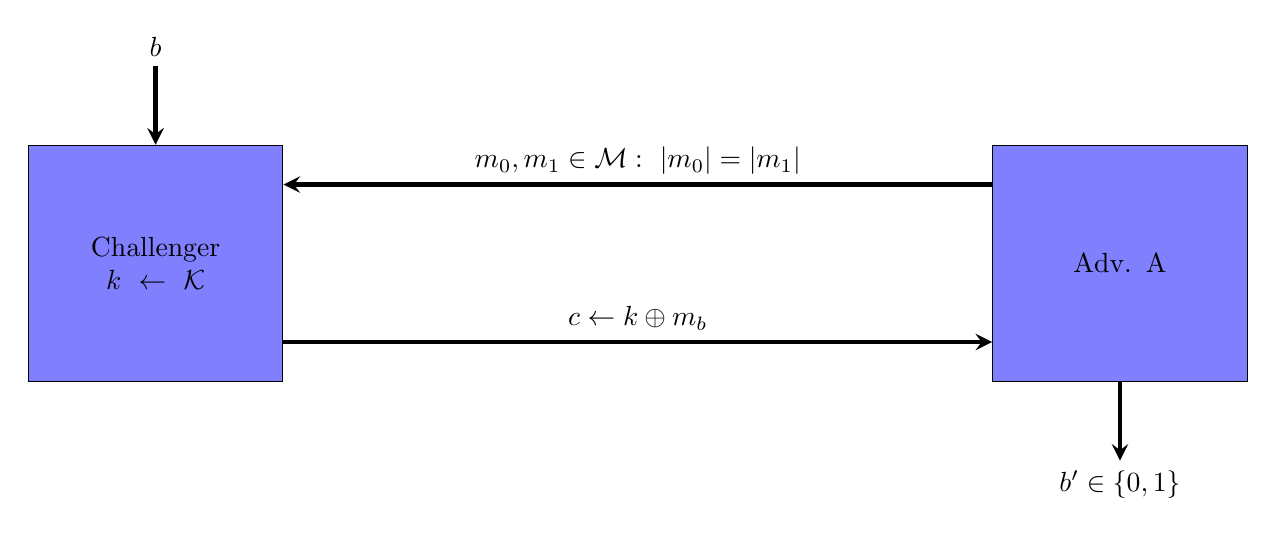
\begin{tikzpicture}
		\node[draw=black,fill=blue!50,minimum size=3cm, text width=3cm,align=center] (chal) {Challenger \ \ $k\leftarrow\mathcal{K}$};
		\node[draw=black,fill=blue!50,minimum size=3cm, text width=3cm,align=center,right=9cm of chal] (adv) {Adv. A};
		\node[shift={(4.5,1.3)}] (ACm) at (chal.east) {$m_{0},m_{1}\in\mathcal{M}:\ |m_{0}|=|m_{1}|$};
		\node[shift={(4.5,-0.7)}] (CAm) at (chal.east) {$c\leftarrow k\oplus m_{b}$};
		\node[above=of chal] (b) {$b$};
		\node[below=of adv] (bl) {$b'\in\{0,1\}$};
		
		\begin{scope}[transform canvas={yshift=1cm}]
			\draw[-stealth, ultra thick] (adv.west)--(chal.east);
		\end{scope}
		\begin{scope}[transform canvas={yshift=-1cm}]
			\draw[-stealth, ultra thick] (chal.east)--(adv.west);
		\end{scope}
		\draw[-stealth,ultra thick] (b.south)--(chal.north);
		\draw[-stealth,ultra thick] (adv.south)--(bl.north);
	\end{tikzpicture}
\end{center}For \textbf{all} $A$:
$$Adv_{SS}[A,\mathcal{E}]=\Big|Pr[A(k\oplus m_{0})=1]-Pr[A(k\oplus m_{1})=1]\Big|=0$$Because the distributions of $k\oplus m_{0}$ and $k\oplus m_{1}$ are the same (this is a property of XOR).

\subsection{Stream Ciphers are Semantically Secure}
\underline{Goal}: Secure PRG $\Rightarrow$ semantically secure stream cipher.
\subsubsection{Stream ciphers are semantically secure}
\Thm $G:\mathcal{K}\rightarrow\{0,1\}^{n}$ is a secure PRG $\Rightarrow$ stream cipher $\mathcal{E}$ derived from $G$ is semantically secure.

%To proof this theorem, we show the contra-positive:
%\begin{center}
%	stream cipher $\mathcal{E}$ derived from $G$ is semantically insecure $\Rightarrow$ $G:\mathcal{K}\rightarrow\{0,1\}^{n}$ is a insecure PRG
%\end{center}
In other words, we are going to show:
$$\forall \text{ semantic secure adversary }A,\ \exists\text{ a PRG adversary }B\text{ (i.e. statistical test) s.t.}$$
$$Adv_{SS}[A,\mathcal{E}]\leq2\cdot Adv_{PRG}[B,G]$$
We know that, if $B$ is an ``efficient'' PRG adversary and $G$ a secure PRG, so $Adv_{PRG}[B,G]$ is ``negligible''. Then, if the inequality above is true, we have that $Adv_{SS}[A,\mathcal{E}]$ is also ``negligible''.

\Proof Let $A$ be a semantic secure adversary.
\begin{center}
	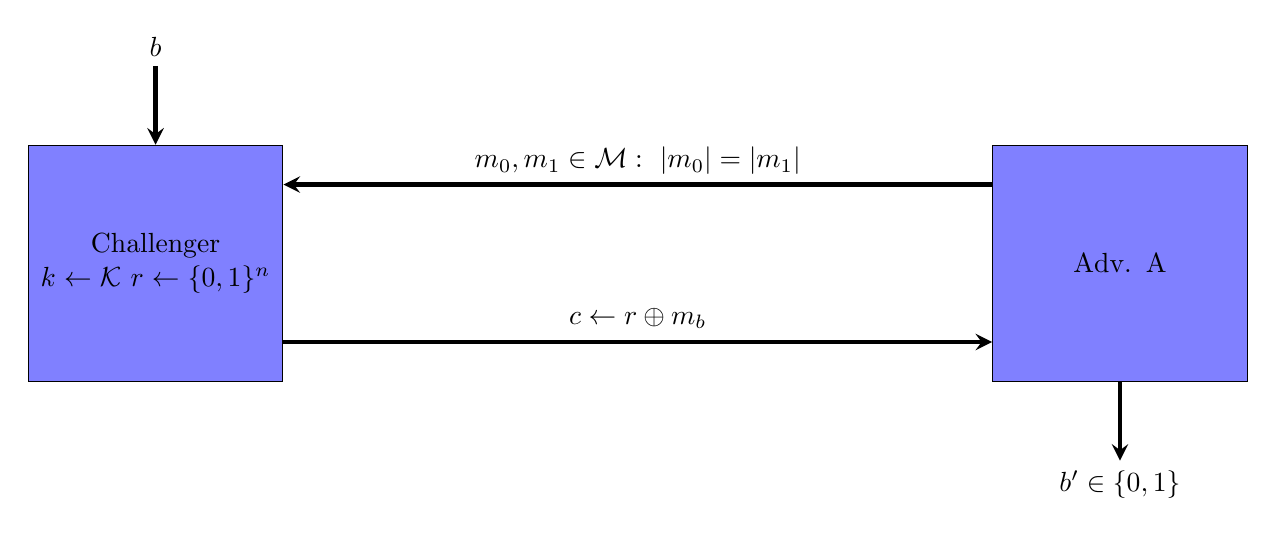
\begin{tikzpicture}
		\node[draw=black,fill=blue!50,minimum size=3cm, text width=3cm,align=center] (chal) {Challenger \ \ $k\leftarrow\mathcal{K}$ $r\leftarrow\{0,1\}^{n}$};
		\node[draw=black,fill=blue!50,minimum size=3cm, text width=3cm,align=center,right=9cm of chal] (adv) {Adv. A};
		\node[shift={(4.5,1.3)}] (ACm) at (chal.east) {$m_{0},m_{1}\in\mathcal{M}:\ |m_{0}|=|m_{1}|$};
		\node[shift={(4.5,-0.7)}] (CAm) at (chal.east) {$c\leftarrow r\oplus m_{b}$};
		\node[above=of chal] (b) {$b$};
		\node[below=of adv] (bl) {$b'\in\{0,1\}$};
		
		\begin{scope}[transform canvas={yshift=1cm}]
			\draw[-stealth, ultra thick] (adv.west)--(chal.east);
		\end{scope}
		\begin{scope}[transform canvas={yshift=-1cm}]
			\draw[-stealth, ultra thick] (chal.east)--(adv.west);
		\end{scope}
		\draw[-stealth,ultra thick] (b.south)--(chal.north);
		\draw[-stealth,ultra thick] (adv.south)--(bl.north);
	\end{tikzpicture}
\end{center}Instead of encrypting using $G(k)$, the challenger we use truly random $r$, but the adversary doesn't knot it. And because the PRG is secure (i.e. indistinguishable of truly random), the adversary can't tell that we made this change. With this, the adversary receives the one time pad encryption.

We know that the adversary's advantage for one time pad is zero, so the if the adversary cannot notice the change, the PRG is secure. But actually, the challenger encrypts the message using $G(k)$.

\begin{center}
	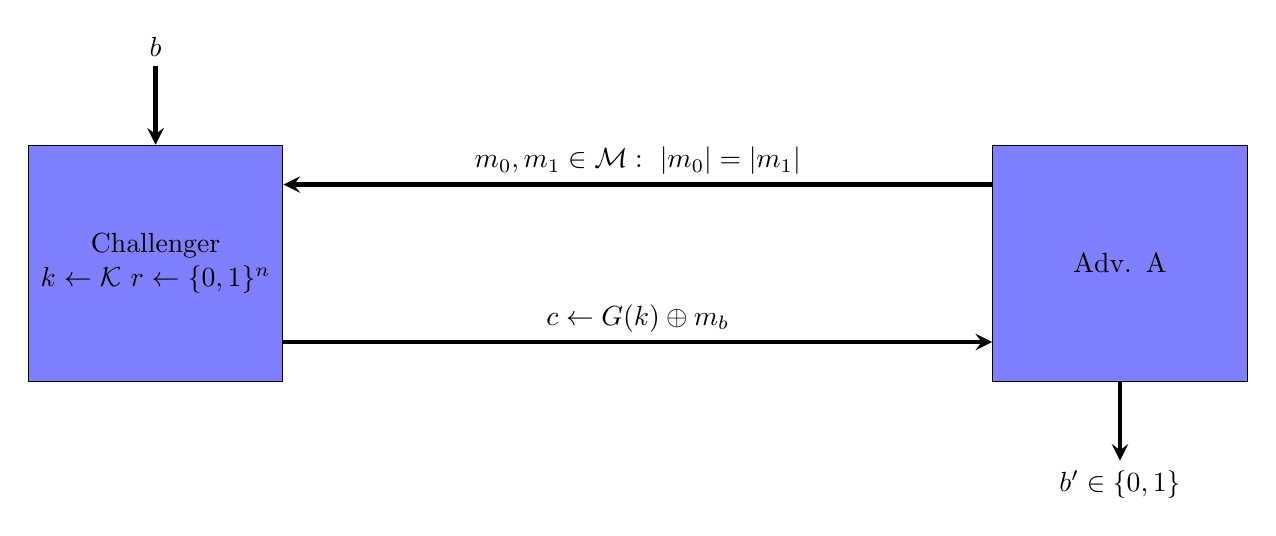
\begin{tikzpicture}
		\node[draw=black,fill=blue!50,minimum size=3cm, text width=3cm,align=center] (chal) {Challenger \ \ $k\leftarrow\mathcal{K}$ $r\leftarrow\{0,1\}^{n}$};
		\node[draw=black,fill=blue!50,minimum size=3cm, text width=3cm,align=center,right=9cm of chal] (adv) {Adv. A};
		\node[shift={(4.5,1.3)}] (ACm) at (chal.east) {$m_{0},m_{1}\in\mathcal{M}:\ |m_{0}|=|m_{1}|$};
		\node[shift={(4.5,-0.7)}] (CAm) at (chal.east) {$c\leftarrow G(k)\oplus m_{b}$};
		\node[above=of chal] (b) {$b$};
		\node[below=of adv] (bl) {$b'\in\{0,1\}$};
		
		\begin{scope}[transform canvas={yshift=1cm}]
			\draw[-stealth, ultra thick] (adv.west)--(chal.east);
		\end{scope}
		\begin{scope}[transform canvas={yshift=-1cm}]
			\draw[-stealth, ultra thick] (chal.east)--(adv.west);
		\end{scope}
		\draw[-stealth,ultra thick] (b.south)--(chal.north);
		\draw[-stealth,ultra thick] (adv.south)--(bl.north);
	\end{tikzpicture}
\end{center}

For $b\in\{0,1\}$: $W_{b}:=[$event that $b'=1]$ and he have that $Adv_{SS}[A,\mathcal{E}]=\Big|Pr[W_{0}]-Pr[W_{1}]\Big|$.\\
When the challenger use $r$ to encrypt, we are going to use:

For $b\in\{0,1\}$: $R_{b}:=[$event that $b'=1]$.

Claim 1: $\Big|Pr[R_{0}]-Pr[R_{1}]\Big|=Adv_{SS}[A,OTP]=0$.

Putting the events on a line:
\begin{center}
	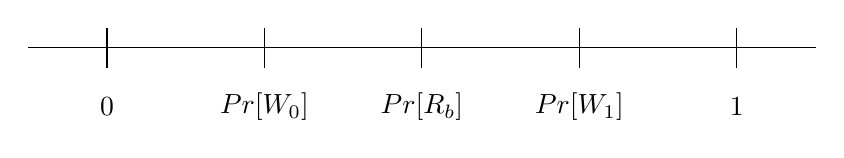
\begin{tikzpicture}
		\draw (0,0)--++(10,0);
		\draw (1,-0.25)--++(0,0.5);
		\draw (3,-0.25)--++(0,0.5);
		\draw (5,-0.25)--++(0,0.5);
		\draw (7,-0.25)--++(0,0.5);
		\draw (9,-0.25)--++(0,0.5);
		
		\node (0) at (1,-0.75) {$0$};
		\node (w0) at (3,-0.75) {$Pr[W_{0}]$};
		\node (rb) at (5,-0.75) {$Pr[R_{b}]$};
		\node (w1) at (7,-0.75) {$Pr[W_{1}]$};
		\node (1) at (9,-0.75) {$1$};
	\end{tikzpicture}
\end{center}We know that $Pr[R_{0}]=Pr[R_{1}]$. and we want to show that the probabilities in the middle of line above are close to each other.

Claim 2: $\exists B:\ \Big|Pr[W_{b}]-Pr[R_{b}]\Big|=Adv_{PRG}[B,G]$, for $b\in\{0,1\}$.

Using the line we know that
$$\Big|Pr[W_{0}]-Pr[R_{b}]\Big|=\Big|Pr[W_{1}]-Pr[R_{b}]\Big|=Adv_{PRG}[B,G]$$
Then, we have that:
$$Adv_{SS}[A,\mathcal{E}]=\Big|Pr[W_{0}]-Pr[W_{1}]\Big|\leq 2\cdot Adv_{PRG}[B,G]$$

Proof of claim 2: $\exists B:\ \Big|Pr[W_{b}]-Pr[R_{b}]\Big|=Adv_{PRG}[B,G]$

Algorithm B:
\begin{center}
	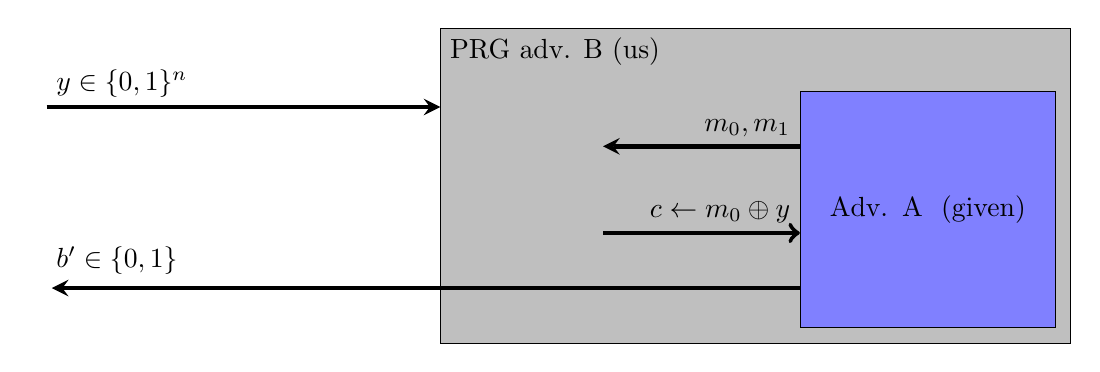
\begin{tikzpicture}
		\node[minimum height=4cm] (empty) {};
		\node[draw=black, fill=gray!50, align=left, right=5cm of empty, minimum height=4cm, minimum width=8cm] (B) {};
		\node[anchor=north west] (Bt) at (B.north west){PRG adv. B (us)};
		\node[draw=black,fill=blue!50,minimum size=3cm, text width=3cm,align=center,anchor=south east,shift={(-0.2,0.2)}] (A) at (B.south east) {Adv. A\ \ (given)};
		
		\begin{scope}[transform canvas={yshift=1cm}]
			\draw[-stealth, ultra thick] (empty.east)--(B.west);
			\node[anchor=south west] (y) at (empty.east){$y\in\{0,1\}^{n}$};
		\end{scope}
		\begin{scope}[transform canvas={yshift=-1cm}]
			\draw[-stealth, ultra thick] (A.west)--++(-9.5,0);
			\node[anchor=south west,shift={(0,-0.25)}] (bl) at (empty.east){$b'\in\{0,1\}$};
		\end{scope}
		\begin{scope}[transform canvas={yshift=0.8cm}]
			\draw[-stealth, ultra thick] (A.west)--++(-2.5,0);
			\node[anchor=south east] (m01) at (A.west){$m_{0},m_{1}$};
		\end{scope}
		\begin{scope}[transform canvas={yshift=-0.3cm}]
			\draw[<-, ultra thick] (A.west)--++(-2.5,0);
			\node[anchor=south east] (m0y) at (A.west){$c\leftarrow m_{0}\oplus y$};
		\end{scope}
	\end{tikzpicture}
\end{center}The advantage of $B$ is:
$$Adv_{PRG}[B,G]=\left|\underset{r\leftarrow\{0,1\}^{n}}{Pr[B(}r)=1]-\underset{k\leftarrow\mathcal{K}}{Pr}[B(G(k))=1]\right|$$But we can say that
$$\underset{r\leftarrow\{0,1\}^{n}}{Pr[B(}r)=1]=Pr[R_{0}]$$and
$$\underset{k\leftarrow\mathcal{K}}{Pr}[B(G(k))=1]=Pr[W_{0}]$$

\chapter{Block Ciphers}
\section{Block Ciphers 1: overview}
\subsection{What are Block Ciphers?}
\subsubsection{Block ciphers: crypto work horse}
\begin{center}
	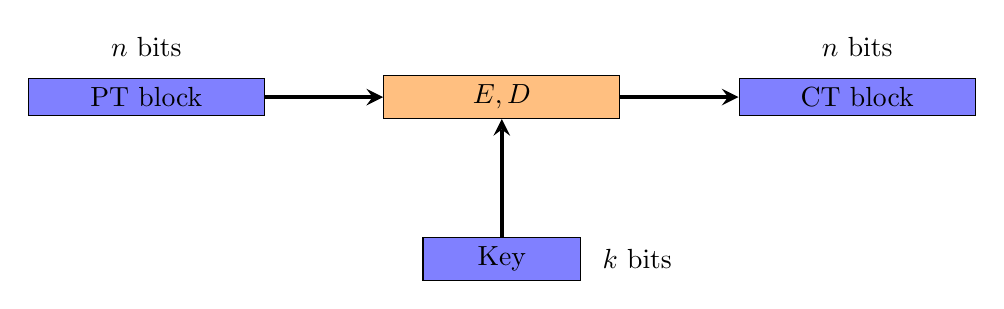
\begin{tikzpicture}
		\node[draw=black, fill=blue!50, minimum width=3cm] (pt) {PT block};
		\node[above=0.15cm of pt] (ptt) {$n$ bits};
		
		\node[draw=black, fill=orange!50, minimum width=3cm, right=1.5cm of pt] (ed) {$E,D$};
		
		\node[draw=black, fill=blue!50, minimum width=3cm, right=1.5cm of ed] (ct) {CT block};
		\node[above=0.15cm of ct] (ctt) {$n$ bits};
		
		\node[draw=black, fill=blue!50, minimum width=2cm, below=1.5cm of ed] (k) {Key};
		\node[right=0.15cm of k] (kt) {$k$ bits};
		
		\draw[-stealth, ultra thick] (pt.east)--(ed.west);
		\draw[-stealth, ultra thick] (ed.east)--(ct.west);
		\draw[-stealth, ultra thick] (k.north)--(ed.south);
	\end{tikzpicture}
\end{center}
There are two canonical examples of block ciphers:
\begin{enumerate}
	\item 3DES: $n=64$ bits, $k=168$ bits
	\item AES: $n=128$ bits, $k=128,\ 192,\ 256$ bits (the longer the key, the slower the cipher is)
\end{enumerate}

\subsubsection{Block Ciphers Built bu Iteration}
\begin{center}
	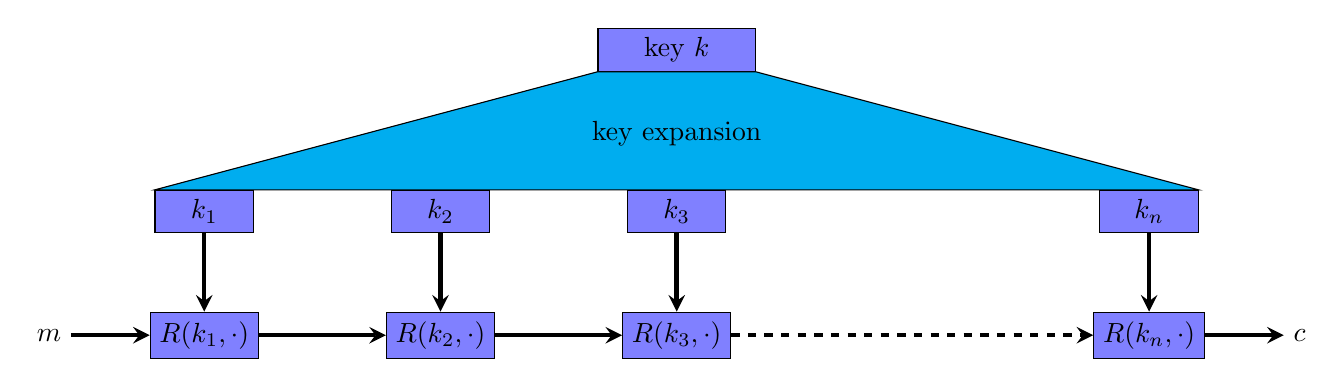
\begin{tikzpicture}
		\node[draw=black,fill=blue!50, minimum width=2cm] (k) {key $k$};
		
		\node[draw=black,fill=blue!50, minimum width=1.25cm, below=1.5cm of k,shift={(-6,0)}] (k1) {$k_{1}$};
		\node[draw=black,fill=blue!50, minimum width=1.25cm, below=1.5cm of k,shift={(-3,0)}] (k2) {$k_{2}$};
		\node[draw=black,fill=blue!50, minimum width=1.25cm, below=1.5cm of k,shift={(0,0)}] (k3) {$k_{3}$};
		\node[draw=black,fill=blue!50, minimum width=1.25cm, below=1.5cm of k,shift={(6,0)}] (kn) {$k_{n}$};
		
		\draw[fill=cyan,draw=black] (k.south west)--(k.south east)--(kn.north east)--(k1.north west)--cycle;
		\node[below=0.5cm of k] (exp) {key expansion};
		
		\node[draw=black,fill=blue!50, minimum width=1.25cm, below=1cm of k1] (rk1) {$R(k_{1},\cdot)$};
		\node[draw=black,fill=blue!50, minimum width=1.25cm, below=1cm of k2] (rk2) {$R(k_{2},\cdot)$};
		\node[draw=black,fill=blue!50, minimum width=1.25cm, below=1cm of k3] (rk3) {$R(k_{3},\cdot)$};
		\node[draw=black,fill=blue!50, minimum width=1.25cm, below=1cm of kn] (rkn) {$R(k_{n},\cdot)$};
		
		\node[left=of rk1] (m) {$m$};
		
		\node[right=of rkn] (c) {$c$};
		
		\draw[-stealth,ultra thick] (k1.south)--(rk1.north);
		\draw[-stealth,ultra thick] (k2.south)--(rk2.north);
		\draw[-stealth,ultra thick] (k3.south)--(rk3.north);
		\draw[-stealth,ultra thick] (kn.south)--(rkn.north);
		\draw[-stealth,ultra thick] (m.east)--(rk1.west);
		\draw[-stealth,ultra thick] (rkn.east)--(c.west);
		\draw[-stealth,ultra thick] (rk1.east)--(rk2.west);
		\draw[-stealth,ultra thick] (rk2.east)--(rk3.west);
		\draw[-stealth,dashed,ultra thick] (rk3.east)--(rkn.west);
	\end{tikzpicture}
\end{center}Where $k_{i}$ are called round keys, $R(k_{i},m_{cs})$ is called a round function and $m_{cs}$ is the current state of the message. And $n=48$ for 3DES and $n=10$ for AES-128.

Block ciphers are slower than stream ciphers, but it's possible to do a lot of stuff that we efficiently can't with some stream ciphers.

\subsubsection{Abstractly: PRPs and PRFs}
An abstraction of a block cipher is called:

\Def Pseudo Random Function (PRF) defined over $(\mathcal{K},\mathcal{X},\mathcal{Y})$:
$$F:\mathcal{K}\times\mathcal{X}\rightarrow\mathcal{Y}$$such that exists ``efficient'' algorithm to evaluate $F(k,x)$, where $\mathcal{K}$ is key space, $\mathcal{X}$ is the input space and $\mathcal{Y}$, the output space. $F$ doesn't need to be invertible.

But there is a related concept that more accurately captures what a block cipher is:

\Def Pseudo Random Permutation (PRP) defined over $(\mathcal{K},\mathcal{X})$:
$$E:\mathcal{K}\times\mathcal{X}\rightarrow\mathcal{X}$$such that:
\begin{enumerate}
	\item Exists ``efficient'' deterministic algorithm to evaluate $E(k,x)$
	\item The function $E(k,\cdot)$ is one-to-one (is invertible, i.e. given one key, there is only a input that matches a output and vice-versa)
	\item Exists ``efficient'' inversion algorithm $D(k,y)$
\end{enumerate}

\subsubsection{Running example}
Example of PRPs: 3DES, AES, ...
\begin{itemize}
	\item[] AES: $\mathcal{K}\times\mathcal{X}\rightarrow\mathcal{X}$ where $\mathcal{K}=\mathcal{X}=\{0,1\}^{128}$
	\item[] 3DES: $\mathcal{K}\times\mathcal{X}\rightarrow\mathcal{X}$ where $\mathcal{X}=\{0,1\}^{64},\ \mathcal{K}=\{0,1\}^{168}$
\end{itemize}

Functionally, any PRP is also a PRF. A PRP is a PRF where $\mathcal{X}=\mathcal{Y}$ and is efficiently invertible.

PRP is a special case of PRF, although that's not entirely accurate.

\subsubsection{Secure PRFs}
Let $F:\mathcal{K}\times\mathcal{X}\rightarrow\mathcal{Y}$ be a PRF
$$\left\{\begin{array}{l}
	Funs[\mathcal{X},\mathcal{Y}]:\ \text{the set of all functions from }\mathcal{X}\text{ to }\mathcal{Y}\\[0.5cm]
	S_{F}=\{F(k,\cdot)\ s.t.\ k\in\mathcal{K}\}\ \subseteq\ Funs[\mathcal{X},\mathcal{Y}]
\end{array}\right.$$
Where $S_{F}$ is the set of all functions from $\mathcal{X}$ to $\mathcal{Y}$ specified by the PRF $F$ as soon as we fix the particular key $k$.

\underline{Intuition}: a PRF is secure if a random function in $Funs[\mathcal{X},\mathcal{Y}]$ is indistinguishable from a random function in $S_{F}$. More precisely, the uniform distribution on the set of pesudorandom functions is indistinguishable from the uniform distribution on the set of all functions.
\begin{center}
	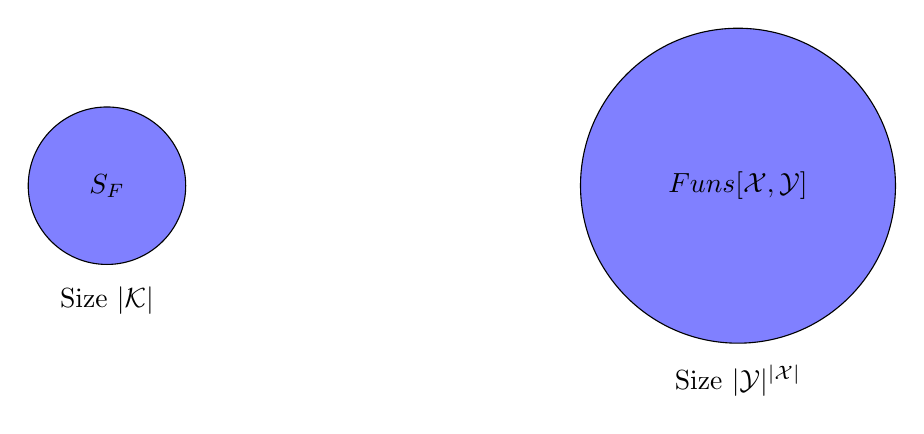
\begin{tikzpicture}
		\node[circle, minimum size=2cm, draw=black,fill=blue!50] (Sf) {$S_{F}$};
		\node[below=0.15cm of Sf] (Sft) {Size $|\mathcal{K}|$};
		
		\node[circle, minimum size=4cm, draw=black,fill=blue!50,right=5cm of Sf] (funs) {$Funs[\mathcal{X},\mathcal{Y}]$};
		\node[below=0.15cm of funs] (funst) {Size $|\mathcal{Y}|^{|\mathcal{X}|}$};
	\end{tikzpicture}
\end{center}

Suppose the attacker makes some inputs $x$ into box that contains a random function $f\in Funs[\mathcal{X},\mathcal{Y}]$ and a PRF $F$ with key $k$. So, the PRF is secure if the attacker can't tell what function the output comes from.

For the PRPs, the definitions are basically the same, with a difference that instead of $Funs[\mathcal{X},\mathcal{Y}]$ is $Perms[\mathcal{X}]$: the set of all one-to-one functions in the set $\mathcal{X}$ (or the set of all invertible functions in the set $\mathcal{X}$).

Example: Let $F:\mathcal{K}\times\mathcal{X}\rightarrow\{0,1\}^{128}$ be secure PRF. The following $G$ is a insecure PRF, because it is easy to distinguish it from a random function: to the input 0 in a random function, the probability of the output be 0 is $\frac{1}{2^{128}}$ and for the function $G$, the probability is $1$.
$$G(k,x)=\left\{\begin{array}{cl}
	0^{128}&if\ x=0\\[0.5cm]
	F(k,x)&otherwise
\end{array}\right.$$

\subsubsection{An easy application: PRF $\Rightarrow$ PRG}
Let $F:\mathcal{K}\times\{0,1\}^{n}\rightarrow\{0,1\}^{n}$ be a secure PRF. Then the following $G:\mathcal{K}\rightarrow\{0,1\}^{nt}$ is a secure PRG:
$$G(k)=F(k,0)\ ||\ F(k,1)\ ||\ \cdots\ ||\ F(k,t)$$

A key property of this generator is that it's parallelizable: if you have two processors or two cores that you can compute on. The you can have one core to compute even entries of the output (second argument of $F$ is even) and another core to compute odd entries of the output. It can run faster.

Security from PRF property: $F(k,\cdot)$ indistinguishable from random function $f(\cdot)$, because it's a secure PRF. So if a build $G$ using the output of a truly random function: $$G(k)=f(0)\ ||\ f(1)\ ||\ \cdots\ ||\ f(t)$$the attacker can't distinguish it from PRG built with the PRF.

\newpage
\section{Block Ciphers 2: The Data Encryption Standard (DES)}
\subsection{The Data Encryption Standard}
\subsubsection{The Data Encryption Standard (DES)}
A little bit of history:
\begin{itemize}
	\item Early 1970s: Horst Feistel designs Lucifer at IBM
	\begin{itemize}
		\item key-len = 128 bits
		\item block-len = 128 bits
	\end{itemize}
	\item 1973: NBS (National Bureau of Standards) asks for block cipher proposals
	\begin{itemize}
		\item IBM submits variant of Lucifer
	\end{itemize}
	\item 1976: NBS adopts DES as a federal standard
	\begin{itemize}
		\item key-len = 56 bits
		\item block-len = 64 bits
	\end{itemize}
	\item 1997: DES broken by exhaustive search
	\item 2000: NIST (National Institute of Standards) adopts Rijndael as AES (Advanced Encryption Standard) to replace DES
\end{itemize}

DES was widely deployed in banking (ACH) an commerce

\subsubsection{DES: core idea -- Feistel Network}
Given arbitrary functions $f_{1},f_{2},\cdots,f_{d}:\ \{0,1\}^{n}\rightarrow\{0,1\}^{n}$ with no need of being invertible.

Goal: build invertible function $F:\{0,1\}^{2n}\rightarrow\{0,1\}^{2n}$

First, we can see the Feistel Network below:
\begin{center}
	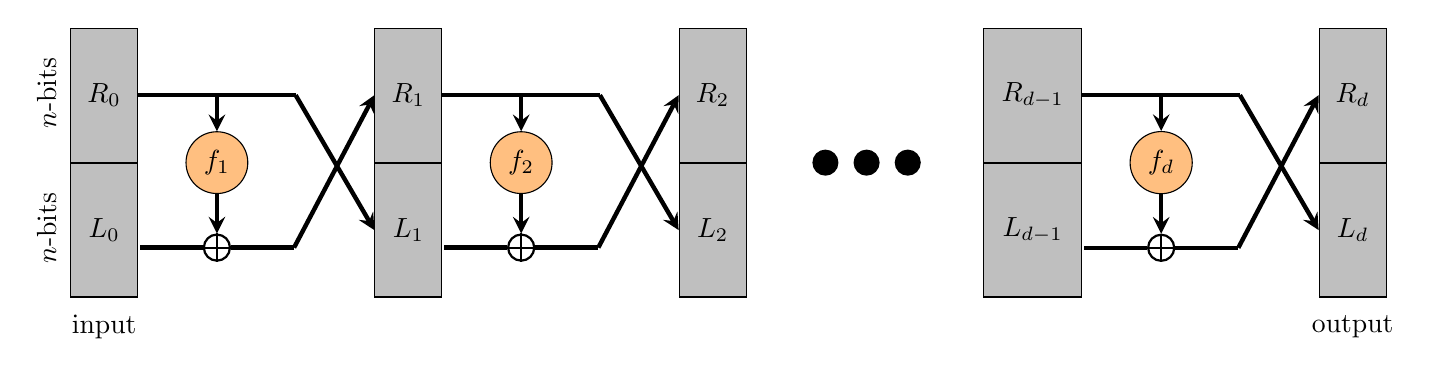
\begin{tikzpicture}
		\node[draw=black,fill=gray!50,minimum width=0.85cm, minimum height=1.7cm] (r0) {$R_{0}$};
		\node[draw=black,fill=gray!50,minimum width=0.85cm, minimum height=1.7cm,anchor=north] (l0) at (r0.south) {$L_{0}$};
		\node[circle,draw=black,fill=orange!50, shift={(1,0)}] (f1) at (r0.south east) {$f_{1}$};
		\node[circle,draw=black,thick,below=0.5cm of f1] (plus1) {};
		\draw[thick] (plus1.north)--(plus1.south);
		\draw[thick] (plus1.west)--(plus1.east);
		\draw[-stealth,ultra thick] (r0.east)-|(f1.north);
		\draw[-stealth,ultra thick] (f1.south)--(plus1.north);
		\draw[ultra thick] (plus1.west)--++(-0.8,0);
		\coordinate[shift={(2,0)}] (rd0) at (r0.east);
		\draw[ultra thick] (r0.east)--(rd0);
		\coordinate[shift={(0.8,0)}] (ld0) at (plus1.east);
		\draw[ultra thick] (plus1.east)--(ld0);
		
		\node[draw=black,fill=gray!50,minimum width=0.85cm, minimum height=1.7cm,right=3cm of r0] (r1) {$R_{1}$};
		\node[draw=black,fill=gray!50,minimum width=0.85cm, minimum height=1.7cm,anchor=north] (l1) at (r1.south) {$L_{1}$};
		\node[circle,draw=black,fill=orange!50, shift={(1,0)}] (f2) at (r1.south east) {$f_{2}$};
		\node[circle,draw=black,thick,below=0.5cm of f2] (plus2) {};
		\draw[thick] (plus2.north)--(plus2.south);
		\draw[thick] (plus2.west)--(plus2.east);
		\draw[-stealth,ultra thick] (r1.east)-|(f2.north);
		\draw[-stealth,ultra thick] (f2.south)--(plus2.north);
		\draw[ultra thick] (plus2.west)--++(-0.8,0);
		\coordinate[shift={(2,0)}] (rd1) at (r1.east);
		\draw[ultra thick] (r1.east)--(rd1);
		\coordinate[shift={(0.8,0)}] (ld1) at (plus2.east);
		\draw[ultra thick] (plus2.east)--(ld1);
		
		\node[draw=black,fill=gray!50,minimum width=0.85cm, minimum height=1.7cm,right=3cm of r1] (r2) {$R_{2}$};
		\node[draw=black,fill=gray!50,minimum width=0.85cm, minimum height=1.7cm,anchor=north] (l2) at (r2.south) {$L_{2}$};
		
		\node[circle,fill=black,shift={(1,0)}] (ret1) at (r2.south east) {};
		\node[circle,fill=black,shift={(0.35,0)}] (ret2) at (ret1.east) {};
		\node[circle,fill=black,shift={(0.35,0)}] (ret3) at (ret2.east) {};
		
		\node[draw=black,fill=gray!50,minimum width=1.25cm, minimum height=1.7cm,right=3cm of r2] (rdm1) {$R_{d-1}$};
		\node[draw=black,fill=gray!50,minimum width=1.25cm, minimum height=1.7cm,anchor=north] (ldm1) at (rdm1.south) {$L_{d-1}$};
		\node[circle,draw=black,fill=orange!50, shift={(1,0)}] (fd) at (rdm1.south east) {$f_{d}$};
		\node[circle,draw=black,thick,below=0.5cm of fd] (plusd) {};
		\draw[thick] (plusd.north)--(plusd.south);
		\draw[thick] (plusd.west)--(plusd.east);
		\draw[-stealth,ultra thick] (rdm1.east)-|(fd.north);
		\draw[-stealth,ultra thick] (fd.south)--(plusd.north);
		\draw[ultra thick] (plusd.west)--++(-0.8,0);
		\coordinate[shift={(2,0)}] (rddm1) at (rdm1.east);
		\draw[ultra thick] (rdm1.east)--(rddm1);
		\coordinate[shift={(0.8,0)}] (lddm1) at (plusd.east);
		\draw[ultra thick] (plusd.east)--(lddm1);
		
		\node[draw=black,fill=gray!50,minimum width=0.85cm, minimum height=1.7cm,right=3cm of rdm1] (rd) {$R_{d}$};
		\node[draw=black,fill=gray!50,minimum width=0.85cm, minimum height=1.7cm,anchor=north] (ld) at (rd.south) {$L_{d}$};
		
		\node[below=0.1 cm of ld] (output) {output};
		\node[below=0.1 cm of l0] (input) {input};
		\node[rotate=90,left=0.3cm of r0,anchor=east,shift={(0.6,0)}] (nbits1) {$n$-bits};
		\node[rotate=90,left=0.3cm of l0,anchor=east,shift={(0.6,0)}] (nbits1) {$n$-bits};
		
		\draw[-stealth,ultra thick] (rd0)--(l1.west);
		\draw[-stealth,ultra thick] (ld0)--(r1.west);
		
		\draw[-stealth,ultra thick] (rd1)--(l2.west);
		\draw[-stealth,ultra thick] (ld1)--(r2.west);
		
		\draw[-stealth,ultra thick] (rddm1)--(ld.west);
		\draw[-stealth,ultra thick] (lddm1)--(rd.west);
	\end{tikzpicture}
\end{center}
Where $R$ is the right part of the word and $L$ is the left.

In symbols, a round of the Feistel Network is given by:
$$\begin{array}{rcl}
	L_{i}&=&R_{i-1}\\[0.2cm]
	R_{i}&=&L_{i-1}\oplus f_{i}(R_{i-1})
\end{array}\ \ \ i=1,\cdots,d$$

\textbf{Claim}: For all $f_{1},f_{2},\cdots,f_{d}:\ \{0,1\}^{n}\rightarrow\{0,1\}^{n}$: Feistel Network $F:\{0,1\}^{2n}\rightarrow\{0,1\}^{2n}$ is efficiently invertible.

\Proof If the following is a round of the Feistel Network
\begin{center}
	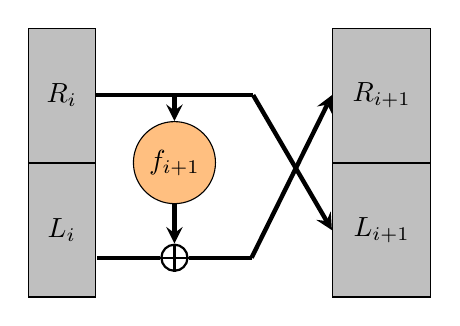
\begin{tikzpicture}
		\node[draw=black,fill=gray!50,minimum width=0.85cm, minimum height=1.7cm] (r1) {$R_{i}$};
		\node[draw=black,fill=gray!50,minimum width=0.85cm, minimum height=1.7cm,anchor=north] (l1) at (r1.south) {$L_{i}$};
		\node[circle,draw=black,fill=orange!50, shift={(1,0)}] (f2) at (r1.south east) {$f_{i+1}$};
		\node[circle,draw=black,thick,below=0.5cm of f2] (plus2) {};
		\draw[thick] (plus2.north)--(plus2.south);
		\draw[thick] (plus2.west)--(plus2.east);
		\draw[-stealth,ultra thick] (r1.east)-|(f2.north);
		\draw[-stealth,ultra thick] (f2.south)--(plus2.north);
		\draw[ultra thick] (plus2.west)--++(-0.8,0);
		\coordinate[shift={(2,0)}] (rd1) at (r1.east);
		\draw[ultra thick] (r1.east)--(rd1);
		\coordinate[shift={(0.8,0)}] (ld1) at (plus2.east);
		\draw[ultra thick] (plus2.east)--(ld1);
		
		\node[draw=black,fill=gray!50,minimum width=1.25cm, minimum height=1.7cm,right=3cm of r1] (r2) {$R_{i+1}$};
		\node[draw=black,fill=gray!50,minimum width=1.25cm, minimum height=1.7cm,anchor=north] (l2) at (r2.south) {$L_{i+1}$};
		
		\draw[-stealth,ultra thick] (rd1)--(l2.west);
		\draw[-stealth,ultra thick] (ld1)--(r2.west);
	\end{tikzpicture}
\end{center}

So the inverse of this round is given by
$$\begin{array}{rcl}
	R_{i}&=&L_{i+1}\\[0.2cm]
	L_{i}&=&R_{i+1}\oplus f_{i+1}(L_{i+1})
\end{array}$$These equations give the following diagram (inverted round)
\begin{center}
	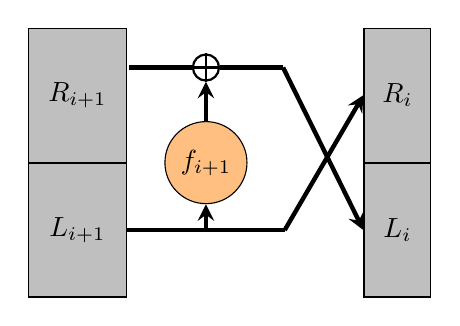
\begin{tikzpicture}
		\node[draw=black,fill=gray!50,minimum width=1.25cm, minimum height=1.7cm] (r1) {$R_{i+1}$};
		\node[draw=black,fill=gray!50,minimum width=1.25cm, minimum height=1.7cm,anchor=north] (l1) at (r1.south) {$L_{i+1}$};
		\node[circle,draw=black,fill=orange!50, shift={(1,0)}] (f2) at (r1.south east) {$f_{i+1}$};
		\node[circle,draw=black,thick,above=0.5cm of f2] (plus2) {};
		\draw[thick] (plus2.north)--(plus2.south);
		\draw[thick] (plus2.west)--(plus2.east);
		\draw[-stealth,ultra thick] (l1.east)-|(f2.south);
		\draw[-stealth,ultra thick] (f2.north)--(plus2.south);
		\draw[ultra thick] (plus2.west)--++(-0.8,0);
		\coordinate[shift={(2,0)}] (ld1) at (l1.east);
		\draw[ultra thick] (l1.east)--(ld1);
		\coordinate[shift={(0.8,0)}] (rd1) at (plus2.east);
		\draw[ultra thick] (plus2.east)--(rd1);
		
		\node[draw=black,fill=gray!50,minimum width=0.85cm, minimum height=1.7cm,right=3cm of r1] (r2) {$R_{i}$};
		\node[draw=black,fill=gray!50,minimum width=0.85cm, minimum height=1.7cm,anchor=north] (l2) at (r2.south) {$L_{i}$};
		
		\draw[-stealth,ultra thick] (rd1)--(l2.west);
		\draw[-stealth,ultra thick] (ld1)--(r2.west);
	\end{tikzpicture}
\end{center}

\subsubsection{Decryption Circuit}
Inversion is basically the same circuit with the inverted rounds applied as a network, with $f_{1},f_{2},\cdots,f_{d}$ applied in reverse order.

If we want to save hardware, we know that the encryption hardware is identical to the decryption hardware with the difference that the functions are applied in the reverse order.

This Feistel mechanism is the general method for building functions (block ciphers) from arbitrary functions. It's used in many block ciphers, but not AES.

\subsubsection{Theorem of Ruby and Rackoff}
\Thm (Luby-Rackoff'85)
$$\begin{array}{cl}
	f:\mathcal{K}\times\{0,1\}^{n}\rightarrow\{0,1\}^{n}\text{ be a secure PRF}\Rightarrow&\\[0.2cm]
	\Rightarrow\text{ 3-round Feistel }F:\mathcal{K}^{3}\times\{0,1\}^{2n}\rightarrow\{0,1\}^{2n}\text{ is a secure PRP}&
\end{array}$$
\begin{center}
	\begin{tikzpicture}
		\node[draw=black,fill=gray!50,minimum width=0.85cm, minimum height=1.7cm] (r0) {$R_{0}$};
		\node[draw=black,fill=gray!50,minimum width=0.85cm, minimum height=1.7cm,anchor=north] (l0) at (r0.south) {$L_{0}$};
		\node[circle,draw=black,fill=orange!50, shift={(1,0)}] (f1) at (r0.south east) {\tiny $f(k_{0},\cdot)$};
		\node[circle,draw=black,thick,below=0.5cm of f1] (plus1) {};
		\draw[thick] (plus1.north)--(plus1.south);
		\draw[thick] (plus1.west)--(plus1.east);
		\draw[-stealth,ultra thick] (r0.east)-|(f1.north);
		\draw[-stealth,ultra thick] (f1.south)--(plus1.north);
		\draw[ultra thick] (plus1.west)--++(-0.8,0);
		\coordinate[shift={(2,0)}] (rd0) at (r0.east);
		\draw[ultra thick] (r0.east)--(rd0);
		\coordinate[shift={(0.8,0)}] (ld0) at (plus1.east);
		\draw[ultra thick] (plus1.east)--(ld0);
		
		\node[draw=black,fill=gray!50,minimum width=0.85cm, minimum height=1.7cm,right=3cm of r0] (r1) {$R_{1}$};
		\node[draw=black,fill=gray!50,minimum width=0.85cm, minimum height=1.7cm,anchor=north] (l1) at (r1.south) {$L_{1}$};
		\node[circle,draw=black,fill=orange!50, shift={(1,0)}] (f2) at (r1.south east) {\tiny $f(k_{1},\cdot)$};
		\node[circle,draw=black,thick,below=0.5cm of f2] (plus2) {};
		\draw[thick] (plus2.north)--(plus2.south);
		\draw[thick] (plus2.west)--(plus2.east);
		\draw[-stealth,ultra thick] (r1.east)-|(f2.north);
		\draw[-stealth,ultra thick] (f2.south)--(plus2.north);
		\draw[ultra thick] (plus2.west)--++(-0.8,0);
		\coordinate[shift={(2,0)}] (rd1) at (r1.east);
		\draw[ultra thick] (r1.east)--(rd1);
		\coordinate[shift={(0.8,0)}] (ld1) at (plus2.east);
		\draw[ultra thick] (plus2.east)--(ld1);
		
		\node[draw=black,fill=gray!50,minimum width=0.85cm, minimum height=1.7cm,right=3cm of r2] (rdm1) {$R_{2}$};
		\node[draw=black,fill=gray!50,minimum width=0.85cm, minimum height=1.7cm,anchor=north] (ldm1) at (rdm1.south) {$L_{2}$};
		\node[circle,draw=black,fill=orange!50, shift={(1,0)}] (fd) at (rdm1.south east) {\tiny $f(k_{2},\cdot)$};
		\node[circle,draw=black,thick,below=0.5cm of fd] (plusd) {};
		\draw[thick] (plusd.north)--(plusd.south);
		\draw[thick] (plusd.west)--(plusd.east);
		\draw[-stealth,ultra thick] (rdm1.east)-|(fd.north);
		\draw[-stealth,ultra thick] (fd.south)--(plusd.north);
		\draw[ultra thick] (plusd.west)--++(-0.8,0);
		\coordinate[shift={(2,0)}] (rddm1) at (rdm1.east);
		\draw[ultra thick] (rdm1.east)--(rddm1);
		\coordinate[shift={(0.8,0)}] (lddm1) at (plusd.east);
		\draw[ultra thick] (plusd.east)--(lddm1);
		
		\node[draw=black,fill=gray!50,minimum width=0.85cm, minimum height=1.7cm,right=3cm of rdm1] (rd) {$R_{3}$};
		\node[draw=black,fill=gray!50,minimum width=0.85cm, minimum height=1.7cm,anchor=north] (ld) at (rd.south) {$L_{3}$};
		
		\node[below=0.1 cm of ld] (output) {output};
		\node[below=0.1 cm of l0] (input) {input};
		\node[rotate=90,left=0.3cm of r0,anchor=east,shift={(0.6,0)}] (nbits1) {$n$-bits};
		\node[rotate=90,left=0.3cm of l0,anchor=east,shift={(0.6,0)}] (nbits1) {$n$-bits};
		
		\draw[-stealth,ultra thick] (rd0)--(l1.west);
		\draw[-stealth,ultra thick] (ld0)--(r1.west);
		
		\draw[-stealth,ultra thick] (rd1)--(ldm1.west);
		\draw[-stealth,ultra thick] (ld1)--(rdm1.west);
		
		\draw[-stealth,ultra thick] (rddm1)--(ld.west);
		\draw[-stealth,ultra thick] (lddm1)--(rd.west);
	\end{tikzpicture}
\end{center}Where $k_{0}$, $k_{1}$ and $k_{2}$ are independent keys.
To be secure means that is indistinguishable from truly random function.

\subsubsection{DES: 16 round Feistel network}
$$f_{1},\cdots,f_{16}:\ \{0,1\}^{32}\rightarrow\{0,1\}^{32},\ \ f_{i}(x)=F(k_{i},x)$$
Where the functions $f_{i}$ are derived from a single function $F$ with different keys $k_{i}$, that's derived from the 56 bit DES key $k$..
\begin{center}
	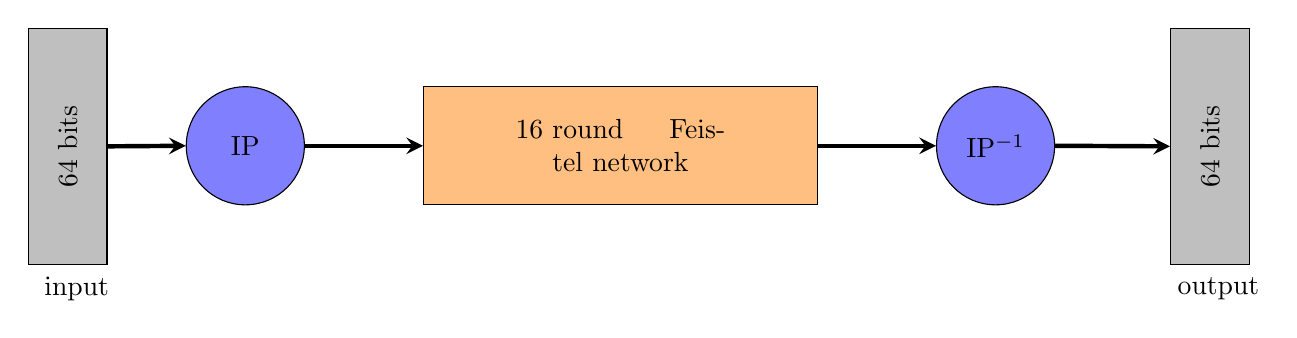
\begin{tikzpicture}
		\node[rotate=90,draw=black,fill=gray!50, minimum width=3cm, minimum height=1cm] (int) {64 bits};
		\node[rotate=90,draw=black,fill=gray!50, minimum width=3cm, minimum height=1cm, right=14cm of int,anchor=north east] (outt) {64 bits};
		\node[circle,draw=black,fill=blue!50,right=1.5cm of int, shift={(0,-1.5)}, minimum size=1.5cm] (ip) {IP};
		\node[draw=black,fill=orange!50,text width=3cm,minimum width=5cm,minimum height=1.5cm,align=center,right=1.5cm of ip] (net) {16 round\ \ \ \ \ Feistel network};
		\node[circle,draw=black,fill=blue!50,right=1.5cm of net, minimum size=1.5cm] (ip1) {IP$^{-1}$};
		
		\node[left=0.2cm of int,shift={(0.85,-0.3)}] (in) {input};
		\node[left=0.2cm of outt,shift={(0.95,-0.3)}] (out) {output};
		
		\draw[-stealth,ultra thick] (int.south)--(ip.west);
		\draw[-stealth,ultra thick] (ip.east)--(net.west);
		\draw[-stealth,ultra thick] (net.east)--(ip1.west);
		\draw[-stealth,ultra thick] (ip1.east)--(outt.north);
	\end{tikzpicture}
\end{center}
IP is a initial permutation that permutes the 64 bits around. It maps bit one to bit 6, bit 2 to bit 17, an so on. This is specified just for standards, not for security. And IP$^{-1}$ is the inverse of the initial permutation.

As said above, the 56 bit key $k$ is expanded into the 16 round keys, where each round key is 48 bits. This expansion will not be described.

To invert the cipher, we just have to use keys in reverse order.

\subsubsection{The function $F(k_{i},x)$}
The following drawing shows the function $F(k_{i},x)$:
\begin{center}
	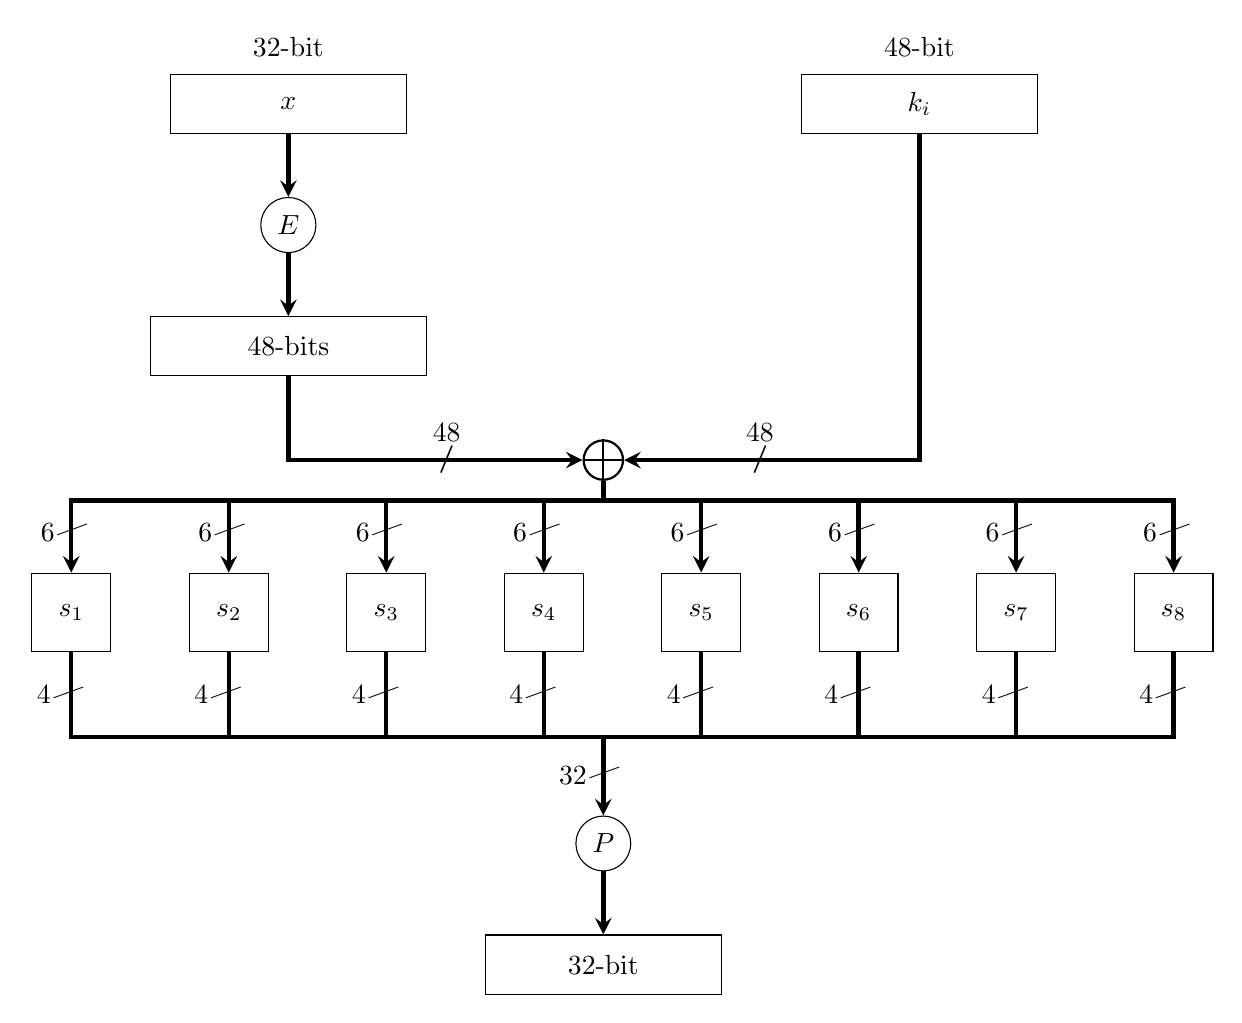
\begin{tikzpicture}
		\node[minimum width=3cm,minimum height=0.75cm,draw=black] (x) {$x$};
		
		\node[minimum width=3cm,minimum height=0.75cm,draw=black,right=5cm of x] (ki) {$k_{i}$};
		
		\node[circle,draw=black,below=0.8cm of x] (e) {$E$};
		
		\node[minimum width=3.5cm, minimum height=0.75cm,draw=black,below=0.8cm of e] (xe) {48-bits};
		
		\node[circle,minimum size=0.5cm,draw=black,below=0.8cm of xe,shift={(4,0)},thick] (plus) {};
		\draw[thick] (plus.east)--(plus.west);
		\draw[thick] (plus.north)--(plus.south);
		
		\coordinate[shift={(-1,-3)}] (s1) at (xe.south west);
		\foreach \idi in {1,...,8}{%
			\idiii{\idi}
			\coordinate[shift={(2*\idii,0)}] (s\idi) at (s1);
			\node[draw=black,minimum size=1cm] (s0\idi) at (s\idi) {$s_{\idi}$};
		}
		
		\draw[-stealth,ultra thick] (x.south)--(e.north);
		\draw[-stealth,ultra thick] (e.south)--(xe.north);
		\draw[-stealth,ultra thick] (xe.south)|-(plus.west);
		\draw[-stealth,ultra thick] (ki.south)|-(plus.east);
		\coordinate[shift={(0,-0.25)}] (ponto) at (plus.south);
		\coordinate[shift={(0,-3)}] (ponto1) at (ponto.south);
		\node[circle,draw=black,below=1cm of ponto1] (p) {$P$};
		\draw[ultra thick] (plus.south)--(ponto);
		\foreach \idi in {1,...,8}{%
			\draw[-stealth,ultra thick] (ponto)-|(s0\idi.north);
			\draw[ultra thick] (s0\idi.south)|-(ponto1);
			\node[above=0.3cm of s0\idi,rotate=20,shift={(0.1,0)}] (a\idi) {\textbf{---}};
			\node[left=0.1cm of a\idi,shift={(0.3,0.1)}] (a0\idi) {6};
			\node[below=0.3cm of s0\idi,rotate=20,shift={(-0.1,0)}] (b\idi) {\textbf{---}};
			\node[left=0.1cm of b\idi,shift={(0.3,0.1)}] (b0\idi) {4};
		}
		\draw[-stealth,ultra thick] (ponto1)--(p.north);
		
		\node[minimum width=3cm,minimum height=0.75cm,draw=black,below=0.8cm of p] (out) {32-bit};
		\draw[-stealth,ultra thick] (p.south)--(out.north);
		
		\node[left=1.5cm of plus] (48t1) {\textbf{/}};
		\node[above=0.01cm of 48t1,shift={(0,-0.2)}] (481) {48};
		\node[right=1.5cm of plus] (48t2) {\textbf{/}};
		\node[above=0.01cm of 48t2,shift={(0,-0.2)}] (482) {48};
		
		\node[above=0.3cm of p,rotate=20,shift={(0.1,0)}] (pt) {\textbf{---}};
		\node[left=0.1cm of pt,shift={(0.3,0.1)}] (pt0) {32};
		
		\node[above=0.1cm of x] (xt) {32-bit};
		\node[above=0.1cm of ki] (kit) {48-bit};
	\end{tikzpicture}
\end{center}
The 32-bit input is expanded to 48 bits. The expansion box $E$ just replicates some bits and moves other bits around. For example, the bit number 1 of the input is replicated into positions 2 and 48 of the expanded input; bit number 2 is positioned in as bit number 3 of the output; an so on. $P$ is another permutation which just maps the bits around (bit number 1 to bit number 9, bit 2 to bit 15 and so on).

\subsubsection{The S-boxes}
The $S$-boxes are functions $\{0,1\}^{6}\rightarrow\{0,1\}^{4}$, implemented as look-up table. For example, the following image shows the look-up table for $S_{5}$.
\begin{figure}[H]
	\centering
	\includegraphics[width=\textwidth]{lut}
\end{figure}Where outer bits are the first and last bits of the input. The painted cell is the output for the input \textcolor{green}{0}\textcolor{orange}{1101}\textcolor{green}{1}.

But how are these $S$-boxes chosen?

\subsubsection{Example: a bad $S$-box choice}
Suppose that the $S$-boxes are linear:
$$S_{i}(x_{1},x_{2},\cdots,x_{6})=\Big(x_{2}\oplus x_{3},x_{1}\oplus x_{4}\oplus x_{5},x_{1}\oplus x_{6},x_{2}\oplus x_{3}\oplus x_{6}\Big)$$or written equivalently: $S_{i}(\mathbf{x})=A_{i}\cdot\mathbf{x}\ (mod\ 2)$:
$$\left[\begin{array}{c}
	x_{2}\oplus x_{3}\\
	x_{1}\oplus x_{4}\oplus x_{5}\\
	x_{1}\oplus x_{6}\\
	x_{2}\oplus x_{3}\oplus x_{6}
\end{array}\right]=\left[\begin{array}{cccccc}
	0&1&1&0&0&0\\
	1&0&0&1&1&0\\
	1&0&0&0&0&1\\
	0&1&1&0&0&1
\end{array}\right]\cdot\left[\begin{array}{c}
	x_{1}\\
	x_{2}\\
	x_{3}\\
	x_{4}\\
	x_{5}\\
	x_{6}
\end{array}\right]\ (mod\ 2)$$If the $S$-boxes are totally linear, then DES is totally insecure.

If the $S$-boxes are linear all DES does is just compute XOR of various things, permute and shuffle bits around. Then all DES is a linear function: $\exists$ fixed binary matrix $B$ s.t.
$$DES(k,m)=B_{64\times 832}\cdot\left[\begin{array}{c}
	m\\
	k_{1}\\
	k_{2}\\
	\vdots\\
	k_{16}
\end{array}\right]=\mathbf{c}\ (mod\ 2)$$

If that happens, we know that, if we XOR 3 outputs of DES, we have:
$$DES(k,m_{1})\oplus DES(k,m_{2})\oplus DES(k,m_{3})=B\left[\begin{array}{c}
	m_{1}\\
	k
\end{array}\right]\oplus B\left[\begin{array}{c}
	m_{2}\\
	k
\end{array}\right]\oplus B\left[\begin{array}{c}
	m_{3}\\
	k
\end{array}\right]=B\left[\begin{array}{c}
	m_{1}\oplus m_{2}\oplus m_{3}\\
	k\oplus k\oplus k
\end{array}\right]$$And as $k\oplus k\oplus k=k$ we have that
$$DES(k,m_{1})\oplus DES(k,m_{2})\oplus DES(k,m_{3})=DES(k,m_{1}\oplus m_{2}\oplus m_{3})$$This relation is not valid for a truly random function. That's why DES is insecure if the $S$-boxes are linear. Because, given enough output pairs, I can literally recover the entire secret key.

\subsubsection{Choosing the $S$-boxes and $P$-box}
If the $S$-boxes were close to linear, in other words, if for 60 of the 64 inputs, the $S$-boxes were linear, it's still enough to break DES.

Choosing the $S$-boxes and $P$-box at random would result in an insecure block cipher (key recovery after $\approx2^{24}$ outputs) [BS'89] Because, the random choices will tend to be somewhat close to linear functions.

Because of this, several rules are used in choice of $S$ and $P$ boxes:
\begin{itemize}
	\item No output bit should be close to linear function of the input bits
	\item $S$-boxes are 4-to-1 maps
	\item[] $\vdots$
\end{itemize}

\subsection{Exhaustive Search Attacks}
\subsubsection{Exhaustive Search for block cipher key}
\textbf{Goal}: given a few input output pairs $\big(m_{i},c_{i}=E(k,m_{i})\big),\ i=1,\cdots,3$, find key $k$.

The first question we have to answer is: how to know if the key is unique? In fact, just one pair is enough to completely constrain a DES key.

\Lemma Suppose DES is an ideal cipher.\footnote{Ideal cipher: pretend that DES is made up of random invertible functions. In other words, for every key, DES implements a random invertible function.} We know that there are $2^{56}$ random invertible functions $\pi_{1},\cdots,\pi_{2^{56}}:\{0,1\}^{64}\rightarrow\{0,1\}^{64}$. We know that DES isn't a collection of $2^{56}$ functions, but we can idealize for our proposes here. Then $\forall m,c$ there is at most one key $k$ s.t. $c=DES(k,m)$ with probability $\geq 1-\frac{1}{256}\approx 99.5\%$.

\Proof We try to find the following probability:
$$Pr[\exists k'\neq k:\ c=DES(k,m)=DES(k',m)]$$What we try to find out is if some key satisfies this probability, so we can limit this probability with the union bound:\footnote{We use the union bound because it's may be the first key (00...0) or the second key (00...1), and so on.}
$$Pr[\exists k'\neq k:\ c=DES(k,m)=DES(k',m)]\leq\sum\limits_{k'\in\{0,1\}^{56}}Pr[DES(k,m)=DES(k',m)]$$The right side of the inequation above are the probabilities of the output of permutation $\pi_{k'}$ be equal to $DES(k,m)$, with $k$ fixed, i.e, $\frac{1}{2^{64}}$. And, as we are summing for all possible keys, we have that:
$$\begin{array}{rcl}
	Pr[\exists k'\neq k:\ c=DES(k,m)=DES(k',m)]&\leq&\sum\limits_{k'\in\{0,1\}^{56}}Pr[DES(k,m)=DES(k',m)]\\[0.6cm]
	&\leq&2^{56}\cdot\frac{1}{2^{64}}=\frac{1}{2^{8}}=\frac{1}{256}
\end{array}$$So the probability that the key is not unique is less than $\frac{1}{256}$. So, the probability that the key is unique is greater than $1-\frac{1}{256}$.

For two DES pairs $\big(m_{1},c_{1}=DES(k,m_{1})\big),\big(m_{2},c_{2}=DES(k,m_{2})\big)$ the unicity probability $\approx1-\frac{1}{2^{71}}$. In other words, given two pairs, it's very likely that only one key will map this pair of messages to this pair of cipher texts. And, it turns out that is possible to find the unique key.

For AES-128: given two in/out pairs, unicity probability $\approx1-\frac{1}{2^{128}}$

Two input/output pairs are enough for exhaustive key search.

How to do exhaustive search: try all the possible keys one by one, until finding the right one.

\subsubsection{DES challenge}
A company supposed a challenge with the initial part of the message known. All the messages are encrypted using the same key $k$.
\begin{center}
	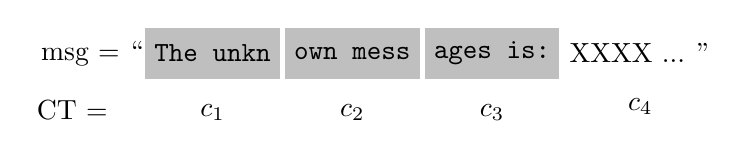
\begin{tikzpicture}
		\node (msg) {msg = ``};
		\node[fill=gray!50,anchor=west,shift={(-0.1,0)},minimum height=0.65cm] (m1) at (msg.east) {\texttt{The unkn}};
		\node[fill=gray!50,anchor=west,shift={(0.05,0)},minimum height=0.65cm] (m2) at (m1.east) {\texttt{own mess}};
		\node[fill=gray!50,anchor=west,shift={(0.05,0)},minimum height=0.65cm] (m3) at (m2.east) {\texttt{ages is:}};
		\node[anchor=west] (xx) at (m3.east) { XXXX ... ''};
		\node[below=0.2cm of msg,align=left,shift={(-0.25,0)}] (ct) {CT =};
		\node[below=0.2cm of m1] (c1) {$c_{1}$};
		\node[below=0.2cm of m2] (c2) {$c_{2}$};
		\node[below=0.2cm of m3] (c3) {$c_{3}$};
		\node[below=0.2cm of xx] (c4) {$c_{4}$};
	\end{tikzpicture}
\end{center}The goal is find $k\in\{0,1\}^{56}$ s.t. $DES(k,m_{i})=c_{i}$ for $i=1,2,3$.

In 1997, by internet search, it took about 3 months to find it.

In 1998, the EFF contracted Paul Kocher to build a special-purpose hardware to break DES (a machine called deep crack that costed about 250k dollars): it took about 3 days to find it.

In 1999, using both Deep Crack and internet search, it took about 22 hours to find it.

Because of this, DES is dead and is no linger secure.

In 2006, a project called COPACABANA (120 FPGAs) took 7 days to find it costing 10k dollars.

So, 56-bit ciphers should not be used!

\subsubsection{Strengthening DES against exhaustive search}
The first idea was to artificially expand the key size. Later, the first idea was iterate the block cipher a couple of times: Triple-DES

Method 1: Triple-DES
\begin{itemize}
	\item Let $E:\mathcal{K}\times \mathcal{M}\rightarrow\mathcal{M}$ be a block cipher
	\item Define $3E:\mathcal{K}^{3}\times\mathcal{M}\rightarrow\mathcal{M}$ as $$3E\big((k_{1},k_{2},k_{3}),m\big)=E\Big(k_{1},D\big(k_{2},E(k_{3},m)\big)\Big)$$where $E$ is the encryption and $D$ the decryption.\footnote{They put a $D$ in the middle just to allow convert the 3DES into the regular DES using $k_{1}=k_{2}=k_{3}$.}
\end{itemize}
For triple-DES: key-size = $3\cdot 56$ = 168 bits and it's 3 times slower than regular DES. Actually, 168 bits is way too long to do an exhaustive search on (time to $2^{168}$). But there is an simple attack in time $\approx 2^{118}$.\footnote{A cipher is considered secure if the time took to be broken is greater than $2^{90}$.}

\subsubsection{Why not double DES?}
Define $2E\big((k_{1},k_{2}),m\big)=E\big(k_{1},E(k_{2},m)\big)$ with key-length of 112 bits. It will be only twice slower than regular DES.

To show that is insecure, lets see the following attack:

We have a bunch of messages $M=(m_{1},\cdots,m_{10})$ and the corresponding cipher texts $C=(c_{1},\cdots,c_{10})$. The goal is to find the pair fo keys $(k_{1},k_{2})$ s.t. $E\big(k_{1},E(k_{2},M)\big)=C$.

Applying the decryption equation we obtain:
$$E(k_{2},M)=D(k_{1},C)$$We separated our variables in two independent sides of equation. That usually means that there is a faster attack than exhaustive search, an attack called meet-in-the-middle attack. The point that this attack attack is the blue point below:
\begin{center}
	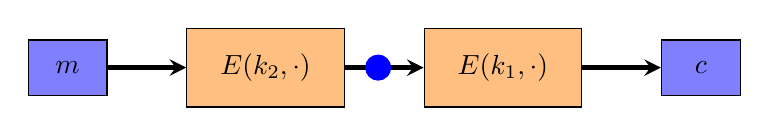
\begin{tikzpicture}
		\node[draw=black,fill=blue!50,minimum height=0.7cm,minimum width=1cm] (m) {$m$};
		\node[draw=black,fill=orange!50,minimum height=1cm,minimum width=2cm,right=of m] (e1) {$E(k_{2},\cdot)$};
		\node[draw=black,fill=orange!50,minimum height=1cm,minimum width=2cm,right=of e1] (e2) {$E(k_{1},\cdot)$};
		\node[draw=black,fill=blue!50,minimum height=0.7cm,minimum width=1cm,right=of e2] (c) {$c$};
		
		\draw[-stealth,ultra thick] (m.east)--(e1.west);
		\draw[-stealth,ultra thick] (e1.east)--(e2.west);
		\draw[-stealth,ultra thick] (e2.east)--(c.west);
		
		\node[circle,fill=blue,right=0.25cm of e1] (point) {};
	\end{tikzpicture}
\end{center}What we try to do is to find the keys that maps $m$ into the value in the blue point and $c$ into the value in the blue point.

First, we build a table with $2^{56}$ entries that, for all the possible values for $k_{2}$, encrypts $m$ under this value.
\begin{center}
	\begin{tabular}{|c|c|}
		\hline
		$k^{0}=00\cdots00$&$E(k^{0},M)$\\
		$k^{1}=00\cdots01$&$E(k^{1},M)$\\
		$k^{2}=00\cdots10$&$E(k^{2},M)$\\
		$\vdots$&$\vdots$\\
		$k^{N}=11\cdots11$&$E(k^{N},M)$\\\hline
	\end{tabular}
\end{center}After, we sort this table based on the second column. This operation will take time about $2^{56}\log(2^{56})$, because of the sort.

Second, using the same table, for all $k\in\{0,1\}^{56}$ we have to test if $D(k,C)$ is in 2$^{nd}$ column. If so, then $E(k^{i},M)=D(k,C)\ \Rightarrow\ (k^{i},k)=(k_{2},k_{1})$.

The running time of this algorithm is:
$$\begin{array}{rcl}
	\text{Time}&=&\text{sort time}+\text{number of searches in table}\times\text{search time}\\[0.2cm]
	&=&2^{56}\log(2^{56})+2^{56}\log(2^{56})<2^{63}<<2^{112},\\[0.2cm]
	\text{space}&\approx&2^{56}
\end{array}$$Not secure, because the time took to broke the cipher is about the same time as the exhaustive attack on regular DES (too little).

The same attack on 3DES takes time$=2^{118}$ and space$\approx2^{56}$.
\begin{center}
	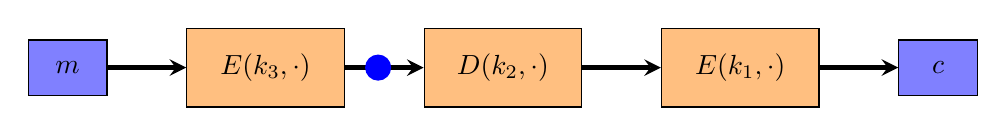
\begin{tikzpicture}
		\node[draw=black,fill=blue!50,minimum height=0.7cm,minimum width=1cm] (m) {$m$};
		\node[draw=black,fill=orange!50,minimum height=1cm,minimum width=2cm,right=of m] (e1) {$E(k_{3},\cdot)$};
		\node[draw=black,fill=orange!50,minimum height=1cm,minimum width=2cm,right=of e1] (e2) {$D(k_{2},\cdot)$};
		\node[draw=black,fill=orange!50,minimum height=1cm,minimum width=2cm,right=of e2] (e3) {$E(k_{1},\cdot)$};
		\node[draw=black,fill=blue!50,minimum height=0.7cm,minimum width=1cm,right=of e3] (c) {$c$};
		
		\draw[-stealth,ultra thick] (m.east)--(e1.west);
		\draw[-stealth,ultra thick] (e1.east)--(e2.west);
		\draw[-stealth,ultra thick] (e2.east)--(e3.west);
		\draw[-stealth,ultra thick] (e3.east)--(c.west);
		
		\node[circle,fill=blue,right=0.25cm of e1] (point) {};
	\end{tikzpicture}
\end{center}Where the blue point is the point of attack.

3DES is in the NIST standard and is actually used quite a bit.

\subsubsection{Strengthening DES against exhaustive search: Method 2: DESX}
This method is not standardized by NIST because it doesn't defend against more subtle attacks on DES. But it's an alternative to 3DES, if we don't want to pay the time and space 3DES takes and we are only worried by the exhaustive search attacks.

Let $E:\mathcal{K}\times\{0,1\}^{n}\rightarrow\{0,1\}^{n}$ be a block cipher. Define $EX$ as
$$EX\big((k_{1},k_{2},k_{3}),m\big)=k_{1}\oplus E(k_{2},m\oplus k_{3})$$
For DESX, the key length is 64+56+64 = 184 bits. 64x2 because of the two XORs and 56 because of the application of the cipher.

This strengthening isn't slower because we apply the cipher once and two additional XORs, which are super fast.

But there is an easy attack in time $2^{64+56}=2^{120}$, which is the best attack known.

There is no exhaustive search attack on this type of construction, but there are more subtle attacks on DES that this construction will not prevent.

Note: If we do only $k_{1}\oplus E(k_{2},m)$ or $E(k_{2},m\oplus k_{1})$ we have nothing. This will be as vulnerable as the regular DES.

\subsection{More Attacks on Block Ciphers}
\subsubsection{Attacks on the implementation}
\textbf{Note}: Never try to implement my own block cipher. Always use the standards: 3DES, AES. And i should never implement crypto primitives by myself

\begin{enumerate}
	\item Side channel attacks:
	\begin{itemize}
		\item Measure time to do encryption/decryption (due to size of the secret key), measure power for enc/dec (it's possible to see what bits belong to the key)
		\begin{figure}[h]
			\centering
			\includegraphics[width=\textwidth]{smartcard}
		\end{figure}The low parts in the graph are the initial permutation (IP) and the reverse (IP$^{-1}$). In the middle we see 16 types of curves which are the 16 rounds. Zooming in the graph, it's possible to recover the bits of key by the power consumed.
	\end{itemize}
	\item Fault attacks:
	\begin{itemize}
		\item Computing errors in the last round expose the secret key $k$. (It's possible to induce errors in the smart card, for example)
		\item It's a good idea to check if the result of the algorithm is correct before outputting it.
	\end{itemize}
\end{enumerate}

\subsubsection{Linear and differential attacks [BS'89, M'93]}
Given many input/output pairs, it's possible to recover key in time less than $2^{56}$ (better than exhaustive search).

\underline{Linear cryptanalysis} (overview): Let $c=DES(k,m)$. Suppose for random $k,m$:
$$Pr\Big[\big(m[i_{1}]\oplus\cdots\oplus m[i_{r}]\big)\oplus\big(c[j_{j}]\oplus\cdots\oplus c[j_{v}]\big)=\big(k[l_{1}]\oplus\cdots\oplus k[l_{u}]\big)\Big]=\frac{1}{2}+\varepsilon$$For some $\varepsilon$. Where, $\big(m[i_{1}]\oplus\cdots\oplus m[i_{r}]\big)$ is a subset of the message bits, $\big(c[j_{j}]\oplus\cdots\oplus c[j_{v}]\big)$ is a subset of the cipher text bits and $\big(k[l_{1}]\oplus\cdots\oplus k[l_{u}]\big)$ is a subset of the key bits. If $m$ and $k$ were independent from each other, the probability would be exactly $\frac{1}{2}$.

For DES, this exists with $\varepsilon=\frac{1}{2^{21}}\approx0.0000000477$. This happens because of a bug in the design of fifth $S$-box, which is too close to a linear function.

\subsubsection{Linear attacks}
We have this following equation:
$$Pr\Big[\big(m[i_{1}]\oplus\cdots\oplus m[i_{r}]\big)\oplus\big(c[j_{j}]\oplus\cdots\oplus c[j_{v}]\big)=\big(k[l_{1}]\oplus\cdots\oplus k[l_{u}]\big)\Big]=\frac{1}{2}+\varepsilon$$

\Thm Given $\frac{1}{\varepsilon^{2}}$ random $\big(m,c=DES(k,m)\big)$ pairs\footnote{$\frac{1}{\varepsilon^{2}}$ is the quantity of random pairs. And the messages $m$ are independent from each other and $c$ are the corresponding cipher texts.} then
$$k[l_{1},\cdots,l_{u}]=MAJ\big[m[i_{1},\cdots,i_{r}]\oplus c[j_{j},\cdots,j_{v}]\big]$$with probability greater than 97.7\%. Where $MAJ$ is the majority of all the values computed (using all the pairs), $k[l_{1},\cdots,l_{u}]$ is the XOR of the key bits, $m[i_{1},\cdots,i_{r}]$ is the XOR of the message bits and $c[j_{j},\cdots,j_{v}]$ is the XOR of the corresponding cipher text bits.

Note: with $\frac{1}{\varepsilon^{2}}$ input/output pairs can find the XOR of key bits in time $\approx\frac{1}{\varepsilon^{2}}$.

For DES, $\varepsilon=\frac{1}{2^{21}}$. So, with $2^{42}$ input/output, it's possible to find $k[l_{1},\cdots,l_{u}]$ in time $2^{42}$.

Roughly speaking: it's possible to find 14 key ``bits'' this way in time $2^{42}$.

By brute force, it's possible to find the remaining $46-14=42$ bits in time $2^{42}$ by exhaustive search.

So, the total attack time is $\approx2^{43}<<2^{56}$ with $2^{42}$ random input/output pair (better than exhaustive search in time, instead of using only 3 pairs in exhaustive search).

\subsubsection{Lesson}
A tiny bit of linearity in $S_{5}$ lead to a $2^{42}$ time attack. So, \textbf{I musn't design ciphers by myself}.

\subsubsection{Quantum attacks}
Quantum attacks are generic attacks on all block ciphers.

Generic search problem:
\begin{itemize}
	\item[] Let $f:\mathcal{X}\rightarrow\{0,1\}$ be a function.
	\item[] Goal: find $x\in\mathcal{X}\ s.t.\ f(x)=1$.
\end{itemize}

The function is given as a black box. In classical computer: best generic algorithm time is $O(|X|)$. In quantum computer [Grover'96]: time is $O(|X|^{\frac{1}{2}})$.

But, can quantum algorithm be built? Unknown.

\subsubsection{Quantum exhaustive search}
Given $m,c=E(k,m)$ define $f(k)=\left\{\begin{array}{ll}
	1&\text{if }E(k,m)=c\\
	0&\text{otherwise}
\end{array}\right.$This function is of the type of function used in quantum computers as seen the subsubsection above.

Grover $\Rightarrow$ quantum computer can find $k$ in time $O(|K|^{\frac{1}{2}})$.
\begin{itemize}
	\item DES: time is $\approx2^{28}$
	\item AES-128: times is $\approx2^{64}$
\end{itemize}Both insecure.

But there is a way: build 256-bits key ciphers, which are secure to quantum attacks (e.g. AES-256)

\newpage
\section{Block Ciphers 3: AES and other constructions}
\subsection{The AES Block Cipher}
\subsubsection{The AES process}
\begin{itemize}
	\item 1997: NIST publishes request for proposal
	\item 1998: 15 submissions. 5 claimed attacks.
	\item 1999: NIST chooses 5 finalists
	\item 2000: NIST chooses Rijndael as AES (designed in Belgium)
\end{itemize}
Key sizes: 128, 195, 256 bits. Block size: 128 bits.

The larger the key size is, the more secure the block cipher is as a pseudo random permutation. But this operations is slower because it has more rounds.

\subsubsection{AES is a Substitution-Permutation network (not Feistel)}
In Fesitel network, half the bits weren't changed in a round. In the Subs-Perm Network, all the bits are changed.
\begin{center}
	\resizebox{\textwidth}{!}{%
		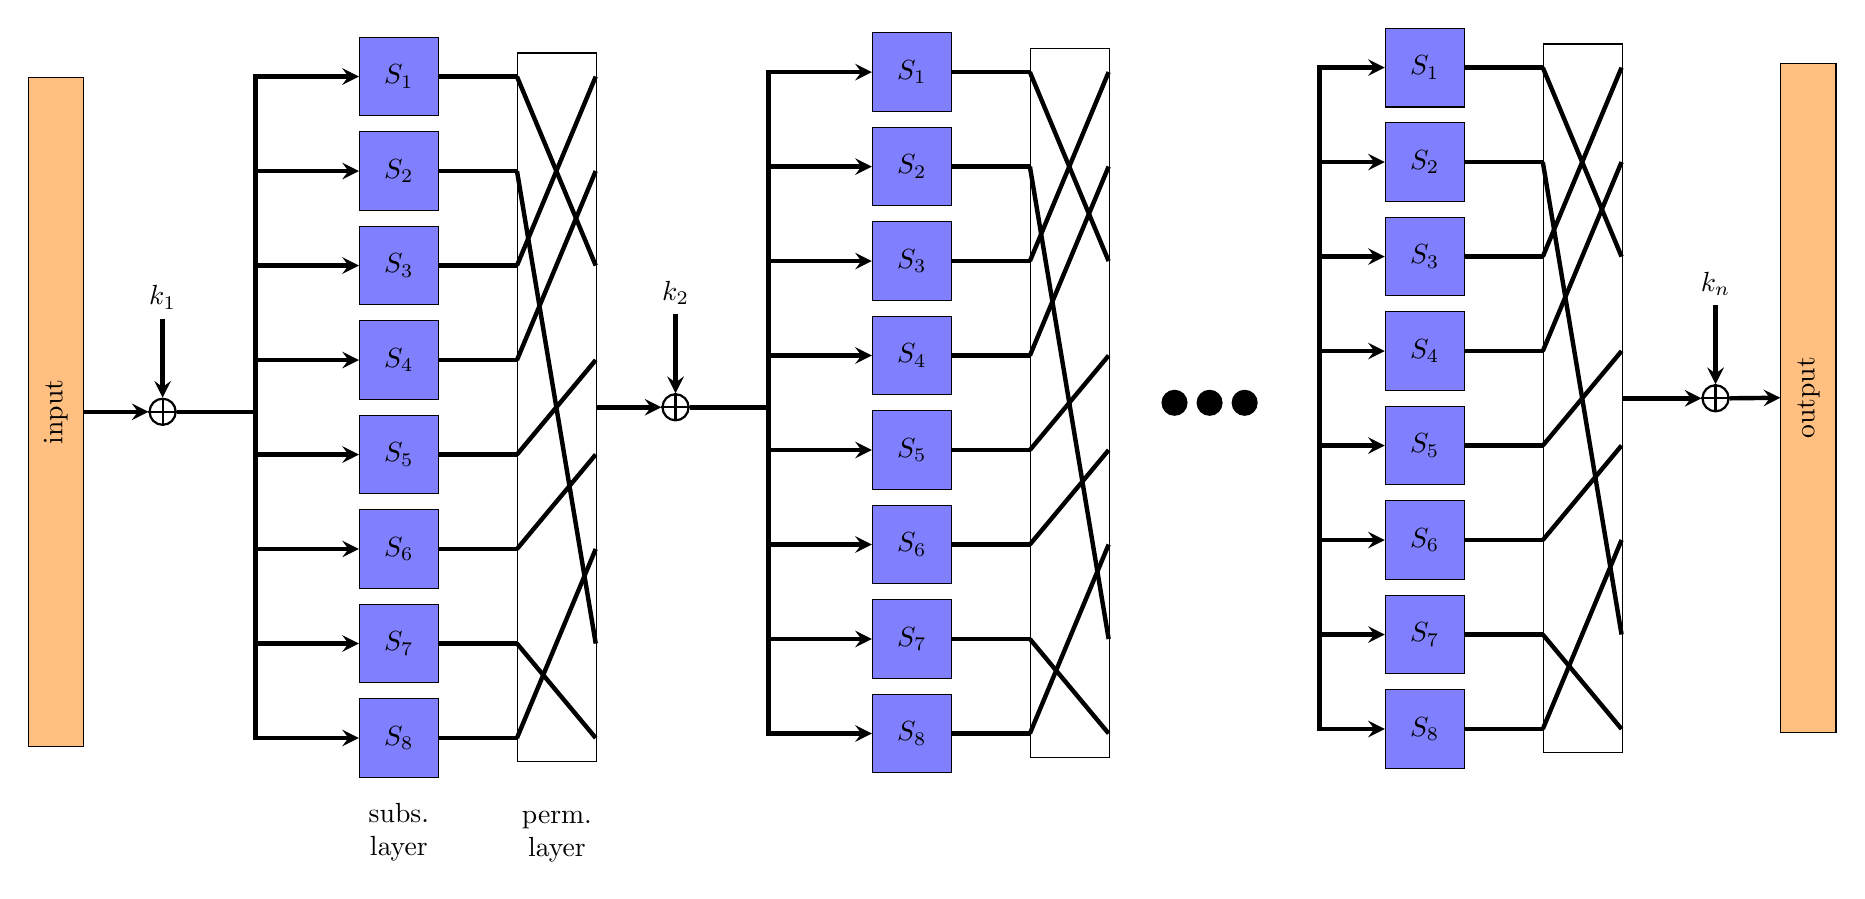
\begin{tikzpicture}
			\node[rotate=90,draw=black,fill=orange!50,minimum height=0.7cm,minimum width=8.5cm] (in) {input};
			\node[circle,draw=black,thick,shift={(1,0)}] (plus) at (in.south) {};
			\draw[thick] (plus.north)--(plus.south);
			\draw[thick] (plus.east)--(plus.west);
			\node[above=of plus] (k1) {$k_{1}$};
			\coordinate[shift={(1,0)}] (p) at (plus.east);
			\coordinate[shift={(4,0)}] (s1) at (in.south east);
			\foreach \idi in {1,...,8}{%
				\idiii{\idi}
				\coordinate[shift={(0,-1.2*\idii)}] (s\idi) at (s1);
				\node[draw=black,fill=blue!50,minimum size=1cm] (s0\idi) at (s\idi) {$S_{\idi}$};
				\draw[-stealth,ultra thick] (p)|-(s0\idi.west);
				\coordinate[shift={(1.5,0)}] (p\idi) at (s\idi);
				\draw[ultra thick] (s0\idi.east)--(p\idi);
				\coordinate[shift={(1,0)}] (q\idi) at (p\idi);
			}
			\node[draw=black,minimum width=1cm,minimum height=9cm,anchor=west,shift={(0,-4.2)}] (permla) at (p1) {};
			\node[text width=1cm,align=center,below=0.2cm of s08] (subs) {subs. layer};
			\node[text width=1cm,align=center,below=0.5cm of permla] (perm) {perm. layer};
			\draw[ultra thick] (p1)--(q3);
			\draw[ultra thick] (p2)--(q7);
			\draw[ultra thick] (p3)--(q1);
			\draw[ultra thick] (p4)--(q2);
			\draw[ultra thick] (p5)--(q4);
			\draw[ultra thick] (p6)--(q5);
			\draw[ultra thick] (p7)--(q8);
			\draw[ultra thick] (p8)--(q6);
			
			\draw[-stealth,ultra thick] (k1.south)--(plus.north);
			\draw[-stealth,ultra thick] (in.south)--(plus.west);
			\draw[ultra thick] (plus.east)--(p.west);
			
			\node[circle,draw=black,thick,shift={(1,0)}] (plus) at (permla.east) {};
			\draw[thick] (plus.north)--(plus.south);
			\draw[thick] (plus.east)--(plus.west);
			\node[above=of plus] (k1) {$k_{2}$};
			\coordinate[shift={(1,0)}] (p) at (plus.east);
			\coordinate[shift={(4,-0.25)}] (s1) at (permla.north east);
			\foreach \idi in {1,...,8}{%
				\idiii{\idi}
				\coordinate[shift={(0,-1.2*\idii)}] (s\idi) at (s1);
				\node[draw=black,fill=blue!50,minimum size=1cm] (s0\idi) at (s\idi) {$S_{\idi}$};
				\draw[-stealth,ultra thick] (p)|-(s0\idi.west);
				\coordinate[shift={(1.5,0)}] (p\idi) at (s\idi);
				\draw[ultra thick] (s0\idi.east)--(p\idi);
				\coordinate[shift={(1,0)}] (q\idi) at (p\idi);
			}
			\node[draw=black,minimum width=1cm,minimum height=9cm,anchor=west,shift={(0,-4.2)}] (permla1) at (p1) {};
			\draw[ultra thick] (p1)--(q3);
			\draw[ultra thick] (p2)--(q7);
			\draw[ultra thick] (p3)--(q1);
			\draw[ultra thick] (p4)--(q2);
			\draw[ultra thick] (p5)--(q4);
			\draw[ultra thick] (p6)--(q5);
			\draw[ultra thick] (p7)--(q8);
			\draw[ultra thick] (p8)--(q6);
			
			\draw[-stealth,ultra thick] (k1.south)--(plus.north);
			\draw[-stealth,ultra thick] (permla.east)--(plus.west);
			\draw[ultra thick] (plus.east)--(p.west);
			
			\node[circle,fill=black,right=0.65cm of permla1] (c1) {};
			\node[circle,fill=black,right=0.1cm of c1] (c2) {};
			\node[circle,fill=black,right=0.1cm of c2] (c3) {};
			
			\coordinate[shift={(8,0)}] (p) at (plus.east);
			\coordinate[shift={(4,-0.25)}] (s1) at (permla1.north east);
			\foreach \idi in {1,...,8}{%
				\idiii{\idi}
				\coordinate[shift={(0,-1.2*\idii)}] (s\idi) at (s1);
				\node[draw=black,fill=blue!50,minimum size=1cm] (s0\idi) at (s\idi) {$S_{\idi}$};
				\draw[-stealth,ultra thick] (p)|-(s0\idi.west);
				\coordinate[shift={(1.5,0)}] (p\idi) at (s\idi);
				\draw[ultra thick] (s0\idi.east)--(p\idi);
				\coordinate[shift={(1,0)}] (q\idi) at (p\idi);
			}
			\node[draw=black,minimum width=1cm,minimum height=9cm,anchor=west,shift={(0,-4.2)}] (permla2) at (p1) {};
			\draw[ultra thick] (p1)--(q3);
			\draw[ultra thick] (p2)--(q7);
			\draw[ultra thick] (p3)--(q1);
			\draw[ultra thick] (p4)--(q2);
			\draw[ultra thick] (p5)--(q4);
			\draw[ultra thick] (p6)--(q5);
			\draw[ultra thick] (p7)--(q8);
			\draw[ultra thick] (p8)--(q6);
			
			\node[circle,draw=black,right=of permla2,thick] (plus) {};
			\draw[thick] (plus.east)--(plus.west);
			\draw[thick] (plus.north)--(plus.south);
			\node[above=of plus] (k1) {$k_{n}$};
			\node[rotate=90,draw=black,fill=orange!50,minimum height=0.7cm,minimum width=8.5cm,right=of plus,shift={(-4.25,0)}] (out) {output};
			
			\draw[-stealth,ultra thick] (k1.south)--(plus.north);
			\draw[-stealth,ultra thick] (permla2.east)--(plus.west);
			\draw[-stealth,ultra thick] (plus.east)--(out.north);
		\end{tikzpicture}
	}
\end{center}
Every step in this network needs to be reversible, so that the whole thing is reversible. So, to decrypt a cipher text, we would take it and apply each step of the network in the reverse order.

The substitution layers are similar to $S$-boxes in DES, but, in this case, they are they have to be reversible.

\subsubsection{AES-128 schematic}
128 bits is the same that 16 bytes. So, the input becomes a 4-by-4 matrix, where each cell contains one byte. The schematic of the AES-128 is shown below.
\begin{center}
	\resizebox{\textwidth}{!}{%
		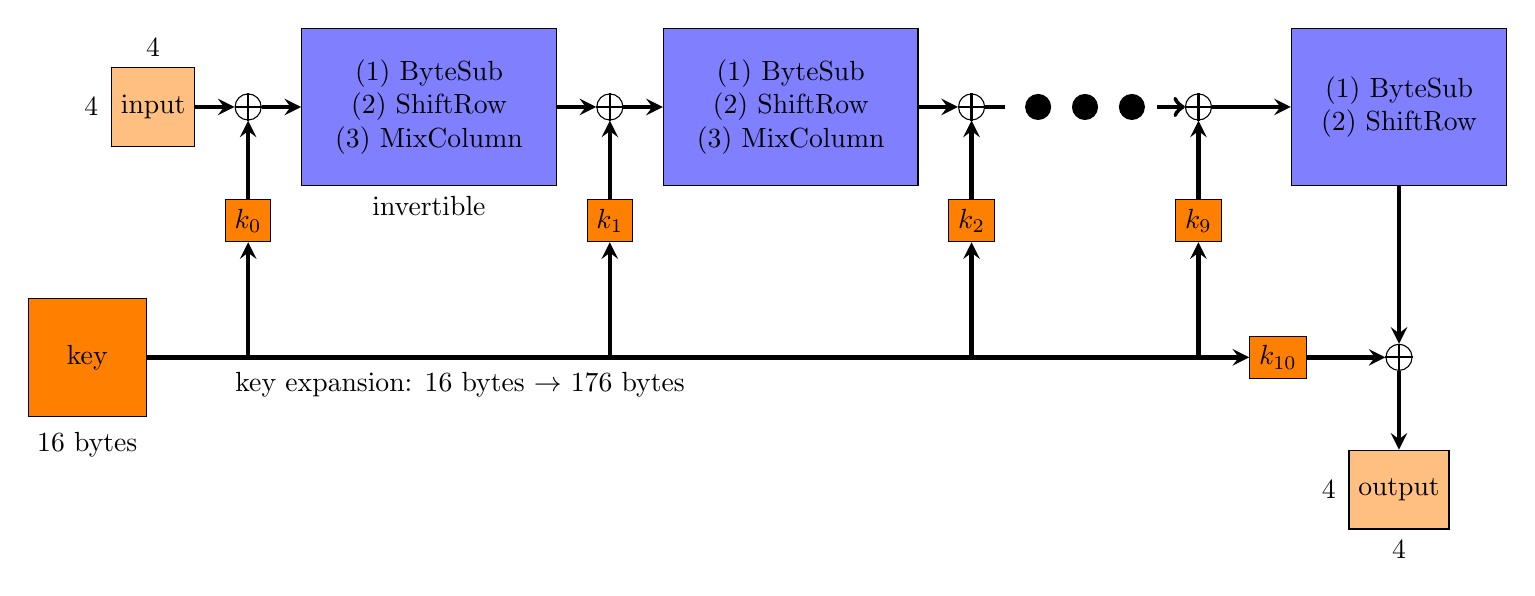
\begin{tikzpicture}
			\node[draw=black,fill=orange!50,minimum height=1cm,minimum width=1cm] (in) {input};
			\node[shift={(-0.25,0)}] (4w) at (in.west){4};
			\node[shift={(0,0.25)}] (4w) at (in.north){4};
			
			\node[circle,draw=black,right=0.5cm of in] (plus) {};
			\draw[thick] (plus.east)--(plus.west);
			\draw[thick] (plus.north)--(plus.south);
			
			\node[draw=black,fill=blue!50,minimum height=2cm,minimum width=3cm,right=0.5cm of plus,text width=3cm,align=center] (round) {(1) ByteSub (2) ShiftRow (3) MixColumn};
			\node[shift={(0,-0.25)}] (inv) at (round.south) {invertible};
			
			\node[below=of plus,draw=black,fill=orange,minimum size=0.5cm] (k0) {$k_{0}$};
			
			\draw[-stealth,ultra thick] (in.east)--(plus.west);
			\draw[-stealth,ultra thick] (plus.east)--(round.west);
			\draw[-stealth,ultra thick] (k0.north)--(plus.south);
			
			\node[circle,draw=black,right=0.5cm of round] (plus) {};
			\draw[thick] (plus.east)--(plus.west);
			\draw[thick] (plus.north)--(plus.south);
			
			\node[draw=black,fill=blue!50,minimum height=2cm,minimum width=3cm,right=0.5cm of plus,text width=3cm,align=center] (round1) {(1) ByteSub (2) ShiftRow (3) MixColumn};
			
			\node[below=of plus,draw=black,fill=orange,minimum size=0.5cm] (k1) {$k_{1}$};
			
			\draw[-stealth,ultra thick] (round.east)--(plus.west);
			\draw[-stealth,ultra thick] (plus.east)--(round1.west);
			\draw[-stealth,ultra thick] (k1.north)--(plus.south);
			
			\node[circle,draw=black,right=0.5cm of round1] (plus) {};
			\draw[thick] (plus.east)--(plus.west);
			\draw[thick] (plus.north)--(plus.south);
			
			\node[below=of plus,draw=black,fill=orange,minimum size=0.5cm] (k2) {$k_{2}$};
			
			\draw[-stealth,ultra thick] (round1.east)--(plus.west);
			\draw[ultra thick] (plus.east)--++(0.25,0);
			\draw[-stealth,ultra thick] (k2.north)--(plus.south);
			
			\node[circle,fill=black,right=0.5cm of plus] (ret1) {};
			\node[circle,fill=black,right=0.25cm of ret1] (ret2) {};
			\node[circle,fill=black,right=0.25cm of ret2] (ret3) {};
			
			\node[circle,draw=black,right=0.5cm of ret3] (plus) {};
			\draw[thick] (plus.east)--(plus.west);
			\draw[thick] (plus.north)--(plus.south);
			
			\node[draw=black,fill=blue!50,minimum height=2cm,minimum width=2.5cm,right=1cm of plus,text width=2.5cm,align=center] (round3) {(1) ByteSub (2) ShiftRow};
			
			\node[below=of plus,draw=black,fill=orange,minimum size=0.5cm] (k9) {$k_{9}$};
			
			\draw[<-,ultra thick] (plus.west)--++(-0.35,0);
			\draw[-stealth,ultra thick] (plus.east)--(round3.west);
			\draw[-stealth,ultra thick] (k9.north)--(plus.south);
			
			\node[circle,draw=black,below=2cm of round3] (plus) {};
			\draw[thick] (plus.east)--(plus.west);
			\draw[thick] (plus.north)--(plus.south);
			
			\node[draw=black,fill=orange!50,minimum height=1cm,minimum width=1cm,below=of plus] (out) {output};
			\node[shift={(-0.25,0)}] (4w) at (out.west){4};
			\node[shift={(0,-0.25)}] (4w) at (out.south){4};
			
			\node[left=of plus,draw=black,fill=orange,minimum size=0.5cm] (k10) {$k_{10}$};
			
			\draw[-stealth,ultra thick] (round3.south)--(plus.north);
			\draw[-stealth,ultra thick] (k10.east)--(plus.west);
			\draw[-stealth,ultra thick] (plus.south)--(out.north);
			
			\node[left=14cm of k10,draw=black,fill=orange,minimum size=1.5cm] (key) {key};
			\node[shift={(0,-0.35)}] (kt) at (key.south) {16 bytes};
			
			\draw[-stealth,ultra thick] (key.east)-|(k0.south);
			\draw[-stealth,ultra thick] (key.east)-|(k1.south);
			\draw[-stealth,ultra thick] (key.east)-|(k2.south);
			\draw[-stealth,ultra thick] (key.east)-|(k9.south);
			\draw[-stealth,ultra thick] (key.east)--(k10.west);
			
			\node[shift={(1,-0.35)},anchor=west] (keyexp) at (key.east) {key expansion: 16 bytes $\rightarrow$ 176 bytes};
		\end{tikzpicture}
	}
\end{center}

\subsubsection{The round function}
\begin{itemize}
	\item ByteSub: a 1 byte $S$-box. 256 byte table (easily computable). It works like this: if its input is a table of 16 cells, like a matrix $A$ with each cell being $a_{i,j}$, $\forall i,j:$ its output will be the matrix $B$, where $b_{i,j}\leftarrow S[a_{i,j}]$. In other words, the substitution table of $S$-box (as a look-up table) is applied to each cell of its input.
	\item Shiftrows: \begin{tabular}{|c|c|c|c|}
		\hline
		$S_{0,0}$&$S_{0,1}$&$S_{0,2}$&$S_{0,3}$\\\hline
		$S_{1,0}$&$S_{1,1}$&$S_{1,2}$&$S_{1,3}$\\\hline
		$S_{2,0}$&$S_{2,1}$&$S_{2,2}$&$S_{2,3}$\\\hline
		$S_{3,0}$&$S_{3,1}$&$S_{3,2}$&$S_{3,3}$\\\hline
	\end{tabular} $\Longrightarrow$ \begin{tabular}{|c|c|c|c|}
		\hline
		$S_{0,0}$&$S_{0,1}$&$S_{0,2}$&$S_{0,3}$\\\hline
		$S_{1,1}$&$S_{1,2}$&$S_{1,3}$&$S_{1,0}$\\\hline
		$S_{2,2}$&$S_{2,3}$&$S_{2,0}$&$S_{2,1}$\\\hline
		$S_{3,3}$&$S_{3,0}$&$S_{3,1}$&$S_{3,2}$\\\hline
	\end{tabular}
	\item MixColumns: A linear transformation is applied independently to each column, in other words, the matrix is multiplied by a certain matrix.
\end{itemize}

\subsubsection{Code size/performance trade-off}
\begin{center}
	\begin{tabular}{N{.3}cN{.2}}
		\hline
		&\textbf{Code size}&\textbf{Performance}\\\hline
		\rowcolor{gray!50}Pre-compute round functions (24KB or 4KB) & largest & fastest: table lookups and XORs\\
		Pre-compute $S$-box only (256 bytes) & smaller & slower\\
		\rowcolor{gray!50}No pre-computation & smallest & slowest\\\hline
	\end{tabular}
\end{center}

\subsubsection{AES in hardware}
AES instructions in Intel Westmere:
\begin{itemize}
	\item \textbf{aesenc}, \textbf{aesenclast}: do one round of AES
	\begin{itemize}
		\item[] 128-bit rgisters: xmm1=state,xmm2=round key
		\item[] aesenc xmm1,xmm2; puts result in xmm1
	\end{itemize}
	\item \textbf{aeskeygenassist}: performs AES key expansion
	\item Claim 14 x speed-up over OpenSSL on same hardware
\end{itemize}
Similar instructions on AMD Bulldozer.

\subsubsection{Attacks}
Best key recovery attack: four times better than exhaustive search [BKE'11]. In other words, instead of 128-bits key attack, it would be a 126 bits attack. But, $2^{126}$ still is a lot of time.

Related key attack on AES-256: [BK'09] Given $2^{99}$ input/output pairs from \textbf{four related keys} in AES-256, it's possible to recover keys in time $2^{99}$.

\subsection{Block Ciphers From PRGs}
\subsubsection{Can we build a PRF from a PRG?}
Let $G:\mathcal{K}\rightarrow\mathcal{K}^{2}$ be a secure PRG, i.e., its output is indistinguishable from a random pick in $\mathcal{K}^{2}$.

Define 1-bit PRF $F:\mathcal{K}\times\{0,1\}\rightarrow\mathcal{K}$ as
$$F(k,x\in\{0,1\})=G(k)[x]$$
\begin{center}
	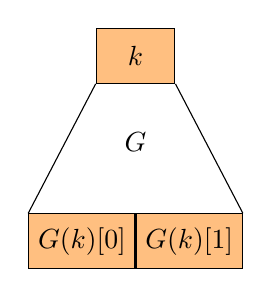
\begin{tikzpicture}
		\node[minimum height=0.7cm,minimum width=1cm,draw=black,fill=orange!50] (k) {$k$};
		
		\node[below=2cm of k,minimum height=0.7cm,minimum width=1cm,draw=black,fill=orange!50,anchor=east] (g0) {$G(k)[0]$};
		
		\node[below=2cm of k,minimum height=0.7cm,minimum width=1cm,draw=black,fill=orange!50,anchor=west] (g1) {$G(k)[1]$};
		
		\node[below=0.5cm of k] (G) {$G$};
		
		\draw (k.south west)--(g0.north west);
		\draw (k.south east)--(g1.north east);
	\end{tikzpicture}
\end{center}
\Thm If $G$ is a secure PRG, then $F$ is a secure PRF.

Note: Remembering that a block cipher is a PRP.

Can we build a PRF with a larger domain? (bigger than 1 bit, as shown above)

\subsubsection{Extending a PRG}
Let $G:\mathcal{K}\rightarrow\mathcal{K}^{2}$ be a secure PRG. Define $G_{1}:\mathcal{K}\rightarrow\mathcal{K}^{4}$ as $$G_{1}(k)=G\big(\textcolor{blue}{G(k)[0]}\big)||G\big(\textcolor{blue}{G(k)[1]}\big)$$
\begin{center}
	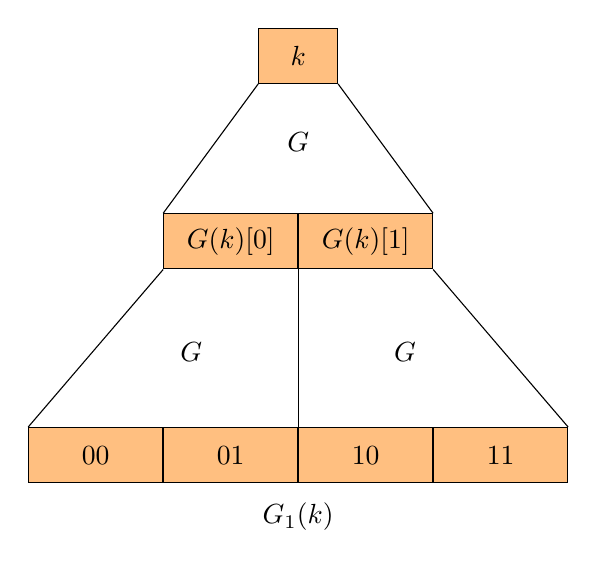
\begin{tikzpicture}
		\node[minimum height=0.7cm,minimum width=1cm,draw=black,fill=orange!50] (k) {$k$};
		
		\node[below=2cm of k,minimum height=0.7cm,minimum width=1.7cm,draw=black,fill=orange!50,anchor=east] (g0) {$G(k)[0]$};
		
		\node[below=2cm of k,minimum height=0.7cm,minimum width=1.7cm,draw=black,fill=orange!50,anchor=west] (g1) {$G(k)[1]$};
		
		\node[below=0.5cm of k] (G) {$G$};
		
		\draw (k.south west)--(g0.north west);
		\draw (k.south east)--(g1.north east);
		
		\node[below=2cm of g0,minimum height=0.7cm,minimum width=1.7cm,draw=black,fill=orange!50] (g00) {01};
		\node[minimum height=0.7cm,minimum width=1.7cm,draw=black,fill=orange!50,anchor=east] (g01) at (g00.west) {00};
		
		\node[below=2cm of g1,minimum height=0.7cm,minimum width=1.7cm,draw=black,fill=orange!50] (g10) {10};
		\node[minimum height=0.7cm,minimum width=1.7cm,draw=black,fill=orange!50,anchor=west] (g11) at (g10.east) {11};
		
		\draw (g0.south west)--(g01.north west);
		\draw (g0.south east)--(g00.north east);
		\draw (g1.south west)--(g10.north west);
		\draw (g1.south east)--(g11.north east);
		
		\node[shift={(-0.5,0.2)},below=of g0] (gt0) {$G$};
		\node[shift={(0.5,0.2)},below=of g1] (gt1) {$G$};
		
		\node[shift={(0,-5.5)}] (G1) at (k.south) {$G_{1}(k)$};
	\end{tikzpicture}
\end{center}
We get a 2-bit PRF: $$F(k,x\in\{0,1\}^{2})=G_{1}(k)[x]$$

We have to show that $G_{1}$ is a secure PRG, in other words, $G_{1}$ is indistinguishable from a random pick in $\mathcal{K}^{4}$.

We know that the first level is secure, i.e., the double $G(k)[0]||G(k)[1]$ is indistinguishable from a random pick in $\mathcal{K}^{2}$. So we have:
\begin{center}
	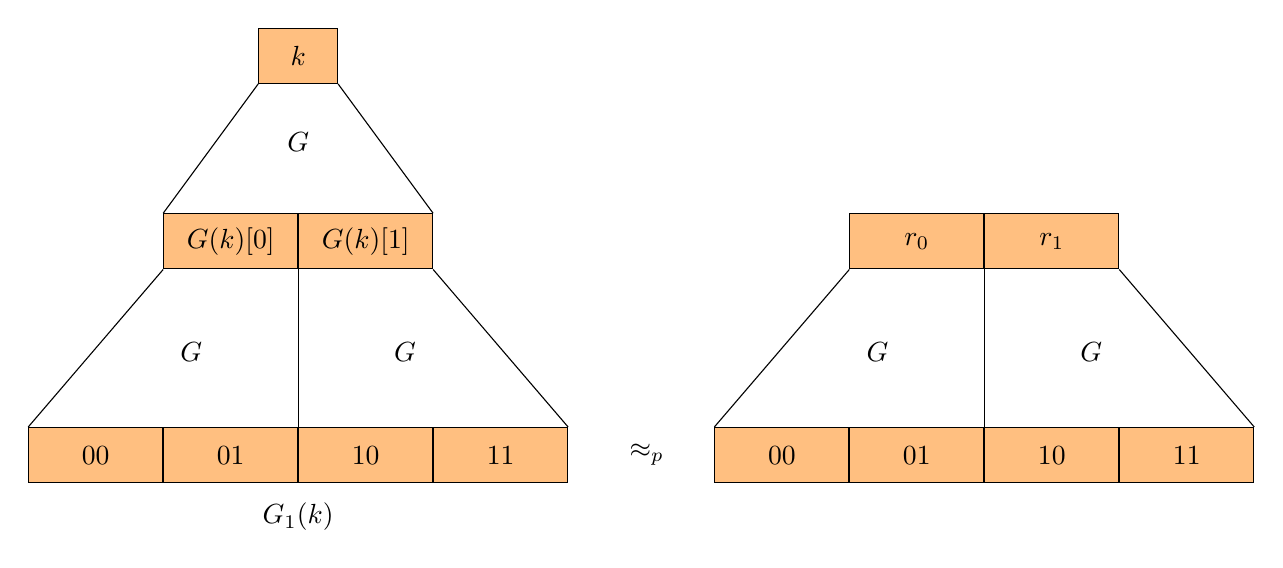
\begin{tikzpicture}
		\node[minimum height=0.7cm,minimum width=1cm,draw=black,fill=orange!50] (k) {$k$};
		
		\node[below=2cm of k,minimum height=0.7cm,minimum width=1.7cm,draw=black,fill=orange!50,anchor=east] (g0) {$G(k)[0]$};
		
		\node[below=2cm of k,minimum height=0.7cm,minimum width=1.7cm,draw=black,fill=orange!50,anchor=west] (g1) {$G(k)[1]$};
		
		\node[below=0.5cm of k] (G) {$G$};
		
		\draw (k.south west)--(g0.north west);
		\draw (k.south east)--(g1.north east);
		
		\node[below=2cm of g0,minimum height=0.7cm,minimum width=1.7cm,draw=black,fill=orange!50] (g00) {01};
		\node[minimum height=0.7cm,minimum width=1.7cm,draw=black,fill=orange!50,anchor=east] (g01) at (g00.west) {00};
		
		\node[below=2cm of g1,minimum height=0.7cm,minimum width=1.7cm,draw=black,fill=orange!50] (g10) {10};
		\node[minimum height=0.7cm,minimum width=1.7cm,draw=black,fill=orange!50,anchor=west] (g11) at (g10.east) {11};
		
		\draw (g0.south west)--(g01.north west);
		\draw (g0.south east)--(g00.north east);
		\draw (g1.south west)--(g10.north west);
		\draw (g1.south east)--(g11.north east);
		
		\node[shift={(-0.5,0.2)},below=of g0] (gt0) {$G$};
		\node[shift={(0.5,0.2)},below=of g1] (gt1) {$G$};
		
		\node[shift={(0,-5.5)}] (G1) at (k.south) {$G_{1}(k)$};
		
		\node[shift={(1,0)}] (eqp) at (g11.east) {$\approx_{p}$};
		
		\node[right=7cm of g1,minimum height=0.7cm,minimum width=1.7cm,draw=black,fill=orange!50,anchor=east] (g0) {$r_{0}$};
		
		\node[minimum height=0.7cm,minimum width=1.7cm,draw=black,fill=orange!50,anchor=west] (g1) at (g0.east) {$r_{1}$};
		
		\node[below=2cm of g0,minimum height=0.7cm,minimum width=1.7cm,draw=black,fill=orange!50] (g00) {01};
		\node[minimum height=0.7cm,minimum width=1.7cm,draw=black,fill=orange!50,anchor=east] (g01) at (g00.west) {00};
		
		\node[below=2cm of g1,minimum height=0.7cm,minimum width=1.7cm,draw=black,fill=orange!50] (g10) {10};
		\node[minimum height=0.7cm,minimum width=1.7cm,draw=black,fill=orange!50,anchor=west] (g11) at (g10.east) {11};
		
		\draw (g0.south west)--(g01.north west);
		\draw (g0.south east)--(g00.north east);
		\draw (g1.south west)--(g10.north west);
		\draw (g1.south east)--(g11.north east);
		
		\node[shift={(-0.5,0.2)},below=of g0] (gt0) {$G$};
		\node[shift={(0.5,0.2)},below=of g1] (gt1) {$G$};
	\end{tikzpicture}
\end{center}Where $r_{0}$ and $r_{1}$ are truly random words in $\mathcal{K}$. And because $G$ is secure, no efficient adversary can distinguish its output from a random pick, so we can do the following change:
\begin{center}
	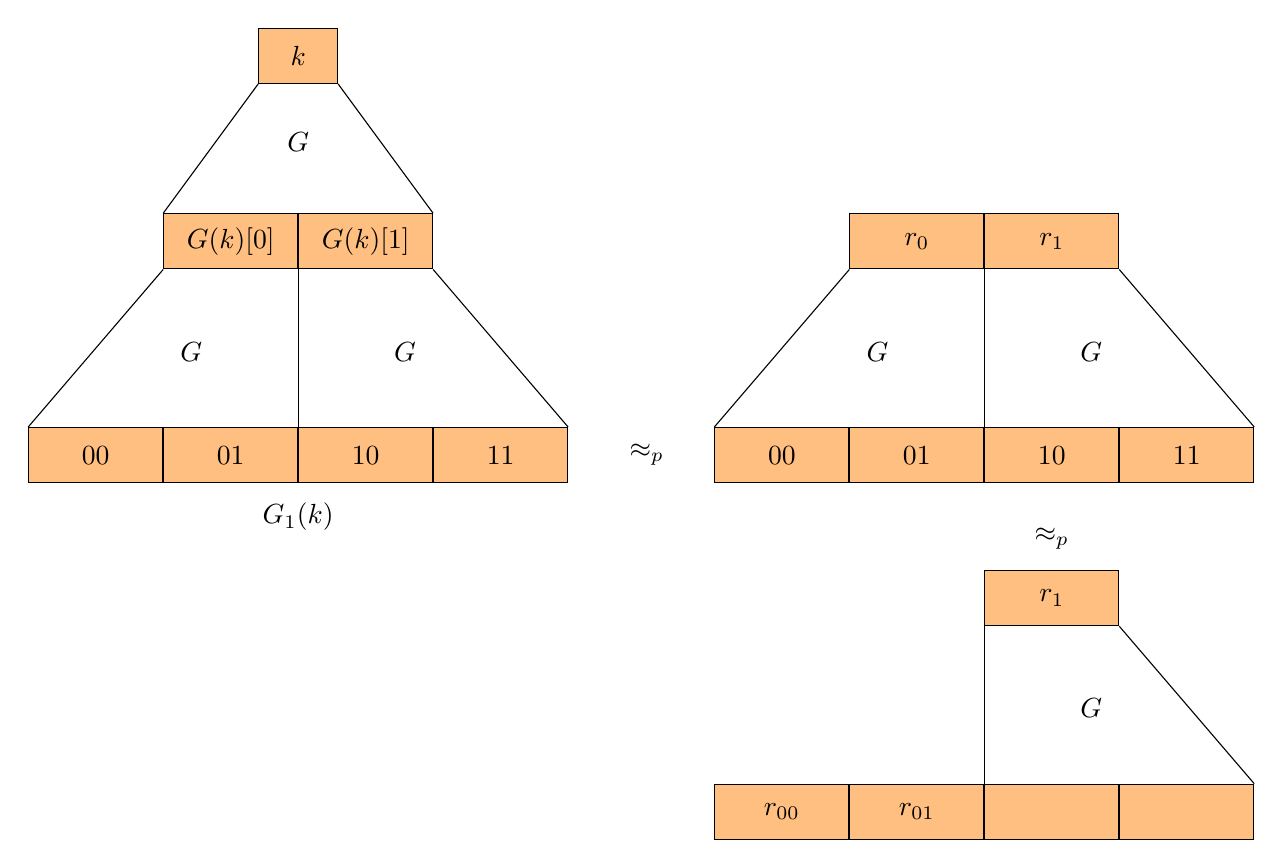
\begin{tikzpicture}
		\node[minimum height=0.7cm,minimum width=1cm,draw=black,fill=orange!50] (k) {$k$};
		
		\node[below=2cm of k,minimum height=0.7cm,minimum width=1.7cm,draw=black,fill=orange!50,anchor=east] (g0) {$G(k)[0]$};
		
		\node[below=2cm of k,minimum height=0.7cm,minimum width=1.7cm,draw=black,fill=orange!50,anchor=west] (g1) {$G(k)[1]$};
		
		\node[below=0.5cm of k] (G) {$G$};
		
		\draw (k.south west)--(g0.north west);
		\draw (k.south east)--(g1.north east);
		
		\node[below=2cm of g0,minimum height=0.7cm,minimum width=1.7cm,draw=black,fill=orange!50] (g00) {01};
		\node[minimum height=0.7cm,minimum width=1.7cm,draw=black,fill=orange!50,anchor=east] (g01) at (g00.west) {00};
		
		\node[below=2cm of g1,minimum height=0.7cm,minimum width=1.7cm,draw=black,fill=orange!50] (g10) {10};
		\node[minimum height=0.7cm,minimum width=1.7cm,draw=black,fill=orange!50,anchor=west] (g11) at (g10.east) {11};
		
		\draw (g0.south west)--(g01.north west);
		\draw (g0.south east)--(g00.north east);
		\draw (g1.south west)--(g10.north west);
		\draw (g1.south east)--(g11.north east);
		
		\node[shift={(-0.5,0.2)},below=of g0] (gt0) {$G$};
		\node[shift={(0.5,0.2)},below=of g1] (gt1) {$G$};
		
		\node[shift={(0,-5.5)}] (G1) at (k.south) {$G_{1}(k)$};
		
		\node[shift={(1,0)}] (eqp) at (g11.east) {$\approx_{p}$};
		
		\node[right=7cm of g1,minimum height=0.7cm,minimum width=1.7cm,draw=black,fill=orange!50,anchor=east] (g0) {$r_{0}$};
		
		\node[minimum height=0.7cm,minimum width=1.7cm,draw=black,fill=orange!50,anchor=west] (g1) at (g0.east) {$r_{1}$};
		
		\node[below=2cm of g0,minimum height=0.7cm,minimum width=1.7cm,draw=black,fill=orange!50] (g00) {01};
		\node[minimum height=0.7cm,minimum width=1.7cm,draw=black,fill=orange!50,anchor=east] (g01) at (g00.west) {00};
		
		\node[below=2cm of g1,minimum height=0.7cm,minimum width=1.7cm,draw=black,fill=orange!50] (g10) {10};
		\node[minimum height=0.7cm,minimum width=1.7cm,draw=black,fill=orange!50,anchor=west] (g11) at (g10.east) {11};
		
		\draw (g0.south west)--(g01.north west);
		\draw (g0.south east)--(g00.north east);
		\draw (g1.south west)--(g10.north west);
		\draw (g1.south east)--(g11.north east);
		
		\node[shift={(-0.5,0.2)},below=of g0] (gt0) {$G$};
		\node[shift={(0.5,0.2)},below=of g1] (gt1) {$G$};
		
		\node[shift={(0,-0.7)}] (eqp) at (g10.south) {$\approx_{p}$};
		
		\node[minimum height=0.7cm,minimum width=1.7cm,draw=black,fill=orange!50,anchor=center,shift={(0,-0.5)}] (g1) at (eqp.south) {$r_{1}$};
		
		\node[below=2cm of g1,minimum height=0.7cm,minimum width=1.7cm,draw=black,fill=orange!50] (g10) {};
		\node[minimum height=0.7cm,minimum width=1.7cm,draw=black,fill=orange!50,anchor=west] (g11) at (g10.east) {};
		
		\node[minimum height=0.7cm,minimum width=1.7cm,draw=black,fill=orange!50,anchor=east] (g01) at (g10.west) {$r_{01}$};
		\node[minimum height=0.7cm,minimum width=1.7cm,draw=black,fill=orange!50,anchor=east] (g00) at (g01.west) {$r_{00}$};
		
		\draw (g1.south west)--(g10.north west);
		\draw (g1.south east)--(g11.north east);
		
		\node[shift={(0.5,0.2)},below=of g1] (gt1) {$G$};
	\end{tikzpicture}
\end{center}
Where $r_{00}$ and $r_{01}$ are truly random words in $\mathcal{K}$. After that, we substitute the remaining pair of words by truly random words and it gets indistinguishable from a random pick in $\mathcal{K}^{4}$.

\subsubsection{Extending more}
Let $G:\mathcal{K}\rightarrow\mathcal{K}^{2}$ be a secure PRG. Define $G_{2}:\mathcal{K}\rightarrow\mathcal{K}^{8}$ as $G_{2}(k)=$
\begin{center}
	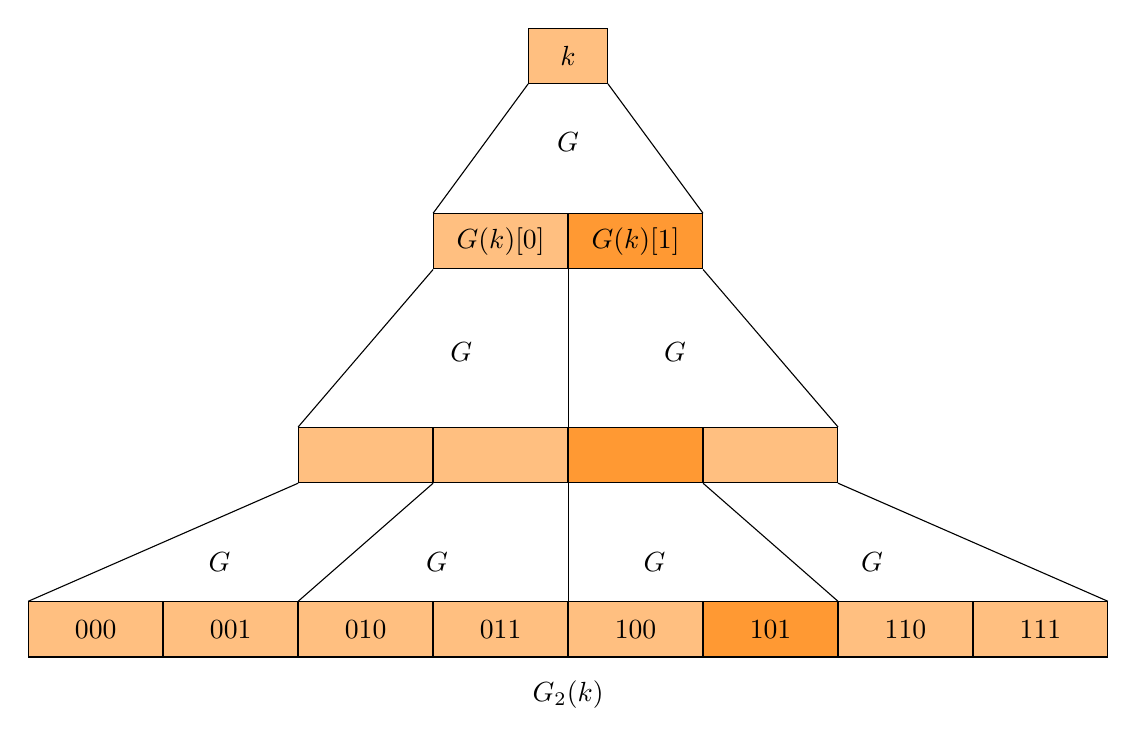
\begin{tikzpicture}
		\node[minimum height=0.7cm,minimum width=1cm,draw=black,fill=orange!50] (k) {$k$};
		
		\node[below=2cm of k,minimum height=0.7cm,minimum width=1.7cm,draw=black,fill=orange!50,anchor=east] (g0) {$G(k)[0]$};
		
		\node[below=2cm of k,minimum height=0.7cm,minimum width=1.7cm,draw=black,fill=orange!80,anchor=west] (g1) {$G(k)[1]$};
		
		\node[below=0.5cm of k] (G) {$G$};
		
		\draw (k.south west)--(g0.north west);
		\draw (k.south east)--(g1.north east);
		
		\node[below=2cm of g0,minimum height=0.7cm,minimum width=1.7cm,draw=black,fill=orange!50] (g00) {};
		\node[minimum height=0.7cm,minimum width=1.7cm,draw=black,fill=orange!50,anchor=east] (g01) at (g00.west) {};
		
		\node[below=2cm of g1,minimum height=0.7cm,minimum width=1.7cm,draw=black,fill=orange!80] (g10) {};
		\node[minimum height=0.7cm,minimum width=1.7cm,draw=black,fill=orange!50,anchor=west] (g11) at (g10.east) {};
		
		\draw (g0.south west)--(g01.north west);
		\draw (g0.south east)--(g00.north east);
		\draw (g1.south west)--(g10.north west);
		\draw (g1.south east)--(g11.north east);
		
		\node[shift={(-0.5,0.2)},below=of g0] (gt0) {$G$};
		\node[shift={(0.5,0.2)},below=of g1] (gt1) {$G$};
		
		\node[minimum height=0.7cm,minimum width=1.7cm,draw=black,fill=orange!50,anchor=west,below=1.5cm of g10] (g100) {100};
		\node[minimum height=0.7cm,minimum width=1.7cm,draw=black,fill=orange!80,anchor=west] (g101) at (g100.east){101};
		\node[minimum height=0.7cm,minimum width=1.7cm,draw=black,fill=orange!50,anchor=west] (g110) at (g101.east){110};
		\node[minimum height=0.7cm,minimum width=1.7cm,draw=black,fill=orange!50,anchor=west] (g111) at (g110.east){111};
		\node[minimum height=0.7cm,minimum width=1.7cm,draw=black,fill=orange!50,anchor=east] (g011) at (g100.west){011};
		\node[minimum height=0.7cm,minimum width=1.7cm,draw=black,fill=orange!50,anchor=east] (g010) at (g011.west){010};
		\node[minimum height=0.7cm,minimum width=1.7cm,draw=black,fill=orange!50,anchor=east] (g001) at (g010.west){001};
		\node[minimum height=0.7cm,minimum width=1.7cm,draw=black,fill=orange!50,anchor=east] (g000) at (g001.west){000};
		
		\draw (g01.south west) -- (g000.north west);
		\draw (g00.south west) -- (g010.north west);
		\draw (g10.south west) -- (g100.north west);
		\draw (g11.south west) -- (g110.north west);
		\draw (g11.south east) -- (g111.north east);
		
		\node[shift={(-1,-1)}] (Gt) at (g01.south west) {$G$};
		\node[shift={(2.5,0)}] (Gt) at (Gt.east) {$G$};
		\node[shift={(2.5,0)}] (Gt) at (Gt.east) {$G$};
		\node[shift={(2.5,0)}] (Gt) at (Gt.east) {$G$};
		
		\node[shift={(0,-7.75)}] (G2) at (k.south) {$G_{2}(k)$};
	\end{tikzpicture}
\end{center}And the proof of security is similar to the one done in the previous section.

We get a 3-bit PRF. And every bit says what side of the output of $G$ we must use, where is the left side and 1 is the right side. For example, the different colors above are of the $F(k,101)$.

\subsubsection{Extending even more: the GGM PRF}
Note: GGM is Goldreich, Goldwasser and Micali, the founders of this construction.

Let $G:\mathcal{K}\rightarrow\mathcal{K}^{2}$ be a secure PRG. Define PRF $F:\mathcal{K}\times\{0,1\}^{n}\rightarrow\mathcal{K}$ as:\\
For input $x=x_{0}x_{1}\cdots x_{n-1}\in\{0,1\}^{n}$ do:
\begin{center}
	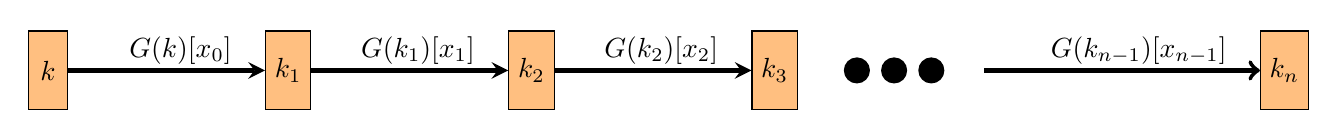
\begin{tikzpicture}
		\node[minimum height=1cm,minimum width=0.5cm,draw=black,fill=orange!50] (k) {$k$};
		
		\node[minimum height=1cm,minimum width=0.5cm,draw=black,fill=orange!50,right=2.5cm of k] (k1) {$k_{1}$};
		\draw[-stealth,ultra thick] (k.east)--(k1.west);
		\node[left=0.3cm of k1,shift={(0,0.25)}] (gt) {$G(k)[x_{0}]$};
		
		\node[minimum height=1cm,minimum width=0.5cm,draw=black,fill=orange!50,right=2.5cm of k1] (k2) {$k_{2}$};
		\draw[-stealth,ultra thick] (k1.east)--(k2.west);
		\node[left=0.3cm of k2,shift={(0,0.25)}] (gt) {$G(k_{1})[x_{1}]$};
		
		\node[minimum height=1cm,minimum width=0.5cm,draw=black,fill=orange!50,right=2.5cm of k2] (k3) {$k_{3}$};
		\draw[-stealth,ultra thick] (k2.east)--(k3.west);
		\node[left=0.3cm of k3,shift={(0,0.25)}] (gt) {$G(k_{2})[x_{2}]$};
		
		\node[circle,fill=black,shift={(0.75,0)}] (ret1) at (k3.east) {};
		\node[circle,fill=black,shift={(0.3,0)}] (ret2) at (ret1.east) {};
		\node[circle,fill=black,shift={(0.3,0)}] (ret3) at (ret2.east) {};
		
		\node[minimum height=1cm,minimum width=0.5cm,draw=black,fill=orange!50,right=4cm of ret3] (kn) {$k_{n}$};
		\draw[<-,ultra thick] (kn.west)--++(-3.5,0);
		\node[left=0.3cm of kn,shift={(0,0.25)}] (gt) {$G(k_{n-1})[x_{n-1}]$};
	\end{tikzpicture}
\end{center}
Where $x_{i}$ its $i$-th bit of $x$. So, the diagram above is how to find $G(k)(x)$ by the way given last section (choosing what side of the output to get). And $k_{i}$ is not a round key, for all $i$ in this example.

\textbf{Security}: $G$ is a secure PRG $\Rightarrow$ F is a secure PRF on $\{0,1\}^{n}$. And the proof is done like before.

This construction is not used in practice due to slow performance.

\newpage
\section{How to Use Block Ciphers 1: one-time key}
\subsection{Review: PRPs and PRFs}
\subsubsection{Secure PRFs}
Let $F:\mathcal{K}\times\mathcal{X}\rightarrow\mathcal{Y}$ be a PRF
$$\left\{\begin{array}{l}
	Funs[\mathcal{X},\mathcal{Y}]:\ \text{the set of all functions from }\mathcal{X}\text{ to }\mathcal{Y}\\[0.5cm]
	S_{F}=\{F(k,\cdot)\ s.t.\ k\in\mathcal{K}\}\ \subseteq\ Funs[\mathcal{X},\mathcal{Y}]
\end{array}\right.$$
Where $S_{F}$ is the set of all functions from $\mathcal{X}$ to $\mathcal{Y}$ specified by the PRF $F$ as soon as we fix the particular key $k$.

\underline{Intuition}: a PRF is secure if a random function in $Funs[\mathcal{X},\mathcal{Y}]$ is indistinguishable from a random function in $S_{F}$. More precisely, the uniform distribution on the set of pesudorandom functions is indistinguishable from the uniform distribution on the set of all functions.
\begin{center}
	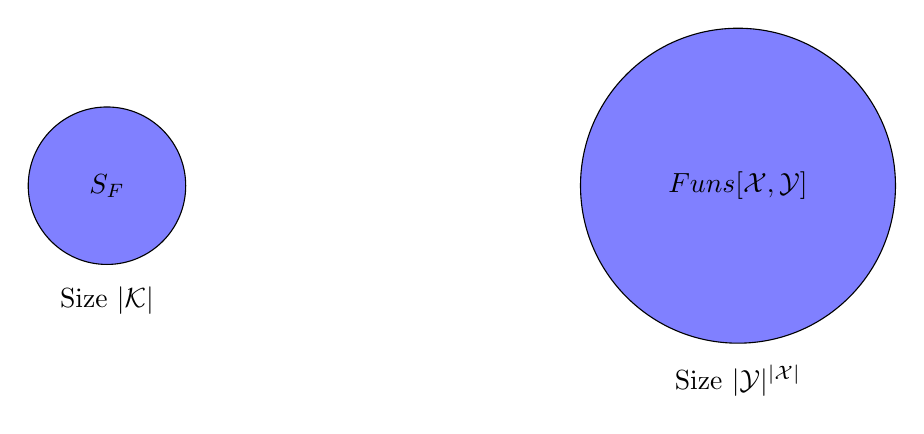
\begin{tikzpicture}
		\node[circle, minimum size=2cm, draw=black,fill=blue!50] (Sf) {$S_{F}$};
		\node[below=0.15cm of Sf] (Sft) {Size $|\mathcal{K}|$};
		
		\node[circle, minimum size=4cm, draw=black,fill=blue!50,right=5cm of Sf] (funs) {$Funs[\mathcal{X},\mathcal{Y}]$};
		\node[below=0.15cm of funs] (funst) {Size $|\mathcal{Y}|^{|\mathcal{X}|}$};
	\end{tikzpicture}
\end{center}

Suppose the attacker makes some inputs $x$ into box that contains a random function $f\in Funs[\mathcal{X},\mathcal{Y}]$ and a PRF $F$ with key $k$. So, the PRF is secure if the attacker can't tell what function the output comes from.

The following diagram shows how to describe if a PRF is secure.\\
For $b\in\{0,1\}$ define experiment $EXP(b)$ as:
\begin{center}
	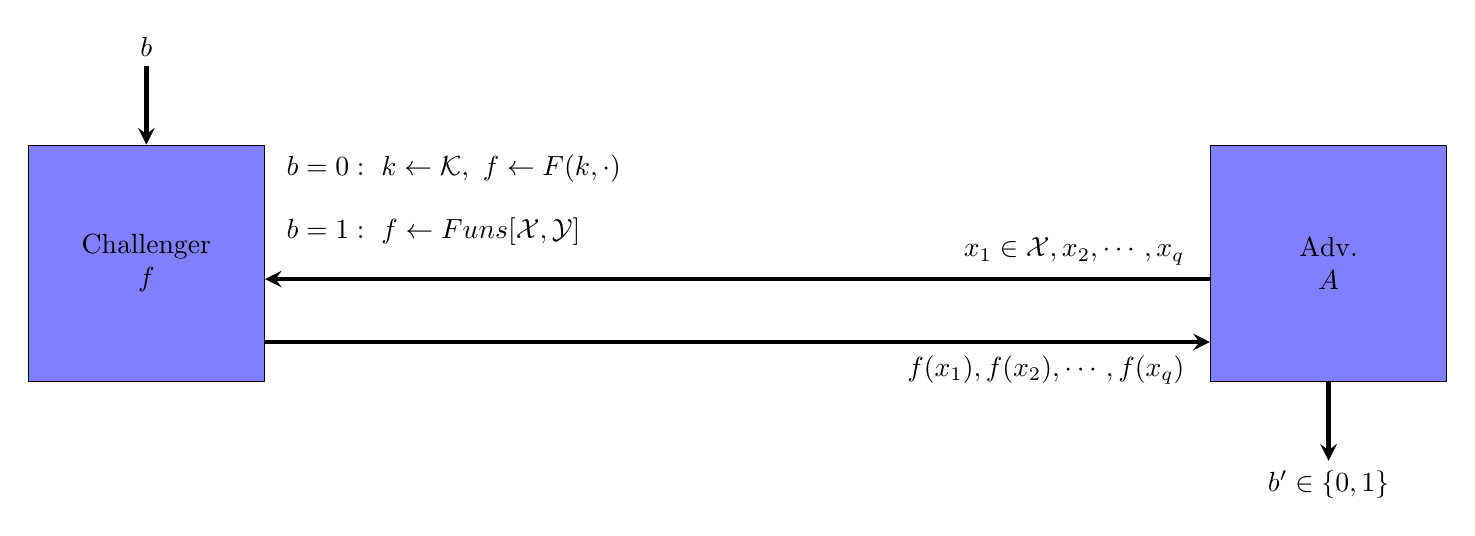
\begin{tikzpicture}
		\node[minimum size=3cm,draw=black,fill=blue!50,text width=2cm,align=center] (chal) {Challenger\ \ $f$};
		
		\node[minimum size=3cm,draw=black,fill=blue!50,text width=1cm,align=center,right=12cm of chal] (adv) {Adv. $A$};
		\begin{scope}[transform canvas={yshift=-1cm}]
			\draw[-stealth,ultra thick] (chal.east)--(adv.west);
			\node[shift={(-0.2,-0.35)},anchor=east] (x1) at (adv.west) {$f(x_{1}),f(x_{2}),\cdots,f(x_{q})$};
		\end{scope}
		\begin{scope}[transform canvas={yshift=-0.2cm}]
			\draw[-stealth,ultra thick] (adv.west)--(chal.east);
			\node[shift={(-0.2,0.35)},anchor=east] (x1) at (adv.west) {$x_{1}\in\mathcal{X},x_{2},\cdots,x_{q}$};
		\end{scope}
		\begin{scope}[transform canvas={yshift=0.4cm}]
			\node[shift={(0.15,0)},anchor=west] (b1) at (chal.east) {$b=1:\ f\leftarrow Funs[\mathcal{X},\mathcal{Y}]$};
		\end{scope}
		\begin{scope}[transform canvas={yshift=1.2cm}]
			\node[shift={(0.15,0)},anchor=west] (b1) at (chal.east) {$b=0:\ k\leftarrow \mathcal{K},\ f\leftarrow F(k,\cdot)$};
		\end{scope}
		\node[above=of chal] (b) {$b$};
		\draw[-stealth,ultra thick] (b.south)--(chal.north);
		
		\node[below=of adv] (bl) {$b'\in\{0,1\}$};
		\draw[-stealth,ultra thick] (adv.south)--(bl.north);
	\end{tikzpicture}
\end{center}Where $b'$ is the output of the adversary $A$ in both $EXP(b=0)$ and $EXP(b=1)$ $\rightarrow$ $b'=EXP(b)$. In other words, $b'$ tries to figure out what $b$ was used. And $x_{1},x_{2},\cdots,x_{q}$ is a $q$-query inputs to challenger.

\Def $F$ is a secure PRF if for all ``efficient'' $A$:
$$Adv_{PRF}[A,F]:=\big|Pr[EXP(0)=1]-Pr[EXP(1)=1]\big|$$is negligible.

\subsubsection{Secure PRP (secure block cipher)}
For the PRPs, the definitions are basically the same, with a difference that instead of $Funs[\mathcal{X},\mathcal{Y}]$ is $Perms[\mathcal{X}]$: the set of all one-to-one functions in the set $\mathcal{X}$ (or the set of all invertible functions in the set $\mathcal{X}$).

For $b\in\{0,1\}$ define experiment $EXP(b)$ as:
\begin{center}
	\begin{tikzpicture}
		\node[minimum size=3cm,draw=black,fill=blue!50,text width=2cm,align=center] (chal) {Challenger\ \ $f$};
		
		\node[minimum size=3cm,draw=black,fill=blue!50,text width=1cm,align=center,right=12cm of chal] (adv) {Adv. $A$};
		\begin{scope}[transform canvas={yshift=-1cm}]
			\draw[-stealth,ultra thick] (chal.east)--(adv.west);
			\node[shift={(-0.2,-0.35)},anchor=east] (x1) at (adv.west) {$f(x_{1}),f(x_{2}),\cdots,f(x_{q})$};
		\end{scope}
		\begin{scope}[transform canvas={yshift=-0.2cm}]
			\draw[-stealth,ultra thick] (adv.west)--(chal.east);
			\node[shift={(-0.2,0.35)},anchor=east] (x1) at (adv.west) {$x_{1}\in\mathcal{X},x_{2},\cdots,x_{q}$};
		\end{scope}
		\begin{scope}[transform canvas={yshift=0.4cm}]
			\node[shift={(0.15,0)},anchor=west] (b1) at (chal.east) {$b=1:\ f\leftarrow Perms[\mathcal{X}]$};
		\end{scope}
		\begin{scope}[transform canvas={yshift=1.2cm}]
			\node[shift={(0.15,0)},anchor=west] (b1) at (chal.east) {$b=0:\ k\leftarrow \mathcal{K},\ f\leftarrow E(k,\cdot)$};
		\end{scope}
		\node[above=of chal] (b) {$b$};
		\draw[-stealth,ultra thick] (b.south)--(chal.north);
		
		\node[below=of adv] (bl) {$b'\in\{0,1\}$};
		\draw[-stealth,ultra thick] (adv.south)--(bl.north);
	\end{tikzpicture}
\end{center}Where $b'$ is the output of the adversary $A$ in both $EXP(b=0)$ and $EXP(b=1)$ $\rightarrow$ $b'=EXP(b)$. In other words, $b'$ tries to figure out what $b$ was used.

\Def $E$ is a secure PRP if for all ``efficient'' $A$:
$$Adv_{PRP}[A,E]:=\big|Pr[EXP(0)=1]-Pr[EXP(1)=1]\big|$$is negligible.

Example: Let $\mathcal{X}=\{0,1\}$. $Perms[\mathcal{X}]$ contains two functions. Consider the following PRP: key space $\mathcal{K}=\{0,1\}$, input space $\mathcal{X}=\{0,1\}$, PRP defined as: $$E(k,x)=x\oplus k$$So, this PRP is secure, because the set of functions $E(k,\cdot)$ is the same of the set $Perms[\mathcal{X}]$, because of the probability of randomly choosing $k$ in $\mathcal{K}$ and randomly choosing a function in $Perms[\mathcal{X}]$.

\subsubsection{Example secure PRPs}
\begin{itemize}
	\item PRPs believed to be secure: 3DES, AES, ...
	\begin{itemize}
		\item[] AES-128: $\mathcal{K}\times\mathcal{X}\rightarrow\mathcal{X}$ where $\mathcal{K}=\mathcal{X}=\{0,1\}^{128}$.
	\end{itemize}
	\item An example concrete assumption about AES:
	\begin{itemize}
		\item[] All $2^{80}$-time algorithms $A$ have $Adv_{PRP}[A,AES]<2^{-40}$
	\end{itemize}
\end{itemize}

Example: Consider the 1-bit PRP from the previous question: $E(k,x)=x\oplus k$. Noting that $Funs[\mathcal{X},\mathcal{X}]$ contains 4 functions (2 invertible functions and 2 functions with constant output). We can say that it is not a secure PRF. Because of the following attack.\\
Attacker $A$:
\begin{itemize}
	\item[] (1) query $f(\cdot)$ at $x=0$ and $x=1$
	\item[] (2) if $f(0)=f(1)$ output ``1'', else ``0''.
	\item[] $Adv_{PRF}[A,E]=|0-\frac{1}{2}|=\frac{1}{2}$ (non negligible)
\end{itemize}

This is only true because the set $\mathcal{X}$ is very small.

\subsubsection{PRF Switching Lemma}
Any secure PRP is also a secure PRF, if $|\mathcal{X}|$ is sufficiently large.

\Lemma Let $E$ be a PRP over $(\mathcal{K},\mathcal{X})$. then for any $q$-query adversary $A$: $$\big|Adv_{PRF}[A,E]-Adv_{PRP}[A,E]\big|<\frac{q^{2}}{2|\mathcal{X}|}$$So if $|\mathcal{X}|$ is large, the difference above is negligible.

The lemma above is the same that: suppose $|\mathcal{X}|$ is large so that $\frac{q^{2}}{2|\mathcal{X}|}$ is ``negligible''. Then $Adv_{PRP}[A,E]$ ``negligible'' $\Rightarrow$ $Adv_{PRF}[A,E]$ ``negligible''.

\subsubsection{Final note}
\begin{itemize}
	\item Suggestion: don't think about the inner-workings of AES and 3DES.
	\item We assume both are secure PRPs and will see how to use them.
	\item From now on, when PRPs and PRFs are mentioned, we are talking about AES and/or 3DES.
\end{itemize}

\subsection{Modes of Operation: One Time Key}
Example of application: encrypted email, new key for every message.
\subsubsection{Using PRPs and PRFs}
\underline{Goal}: build ``secure'' encryption from a secure PRP (e.g. AES).

This segment: one-time keys.
\begin{enumerate}
	\item Adversary's power: Adv sees only one cipher text (one-time key)
	\item Adversary's goal: learn info about plain text from cipher text (break semantic security)
\end{enumerate}
Next segment: many-time keys (a.k.a chosen-plain text security)

\subsubsection{Incorrect use of a PRP}
Electronic Code Book (ECB):
\begin{center}
	\begin{tikzpicture}
		\node (pt) {PT:};
		\node[below=of pt] (ct) {CT:};
		
		\node[draw=black,minimum width=1cm,minimum height=0.7cm,shift={(1,0)}] (p1) at (pt.east){};
		\foreach \idi in {2,...,15}{%
			\idiii{\idi}
			\node[draw=black,minimum width=1cm,minimum height=0.7cm,shift={(\idii,0)}] (p\idi) at (pt.east) {};
		}
		
		\node[draw=black,minimum width=1cm,minimum height=0.7cm,shift={(1,0)}] (c1) at (ct.east){};
		\foreach \idi in {2,...,15}{%
			\idiii{\idi}
			\node[draw=black,minimum width=1cm,minimum height=0.7cm,shift={(\idii,0)}] (c\idi) at (ct.east) {};
		}
		
		\node (m1) at (p4.center) {$m_{1}$};
		\node (cm1) at (c4.center) {$c_{1}$};
		\node (m2) at (p7.center) {$m_{2}$};
		\node (cm2) at (c7.center) {$c_{2}$};
		
		\node[rotate=-90,shift={(0.5,0)}] (arrow) at (p9.south) {$\Rightarrow$};
	\end{tikzpicture}
\end{center}
The problem is: if $m_{1}=m_{2}$ then $c_{1}=c_{2}$.


This problem can be seen when applied to pictures:
\begin{figure}[H]
	\centering
	\includegraphics[width=\textwidth]{ecb}
\end{figure}We see that the silhouette of the man appears in the encrypted image.

So how can we correctly use block ciphers to encrypt long messages?

\subsubsection{Semantic Security (one-time key)}
Let the experiment $EXP(b)$ be, where $b\in\{0,1\}$:
\begin{center}
	\begin{tikzpicture}
		\node[minimum size=3cm,draw=black,fill=blue!50,text width=2cm,align=center] (chal) {Challenger\ \ $k\leftarrow \mathcal{K}$};
		
		\node[minimum size=3cm,draw=black,fill=blue!50,text width=1cm,align=center,right=8cm of chal] (adv) {Adv. $A$};
		\begin{scope}[transform canvas={yshift=-1cm}]
			\draw[-stealth,ultra thick] (chal.east)--(adv.west);
			\node[shift={(-2.7,-0.35)},anchor=east] (x1) at (adv.west) {$c\leftarrow E(k,m_{b})$};
		\end{scope}
		\begin{scope}[transform canvas={yshift=-0.2cm}]
			\draw[-stealth,ultra thick] (adv.west)--(chal.east);
			\node[shift={(-3.2,0.35)},anchor=center] (x1) at (adv.west) {$m_{0},m_{1}\in\mathcal{M}:\ |m_{0}|=|m_{1}|$};
		\end{scope}
		\node[above=of chal] (b) {$b$};
		\draw[-stealth,ultra thick] (b.south)--(chal.north);
		
		\node[below=of adv] (bl) {$b'\in\{0,1\}$};
		\draw[-stealth,ultra thick] (adv.south)--(bl.north);
	\end{tikzpicture}
\end{center}
$$Adv_{SS}[A,OTP]=\big|Pr[EXP(0)=1]-Pr[EXP(1)=1]\big|$$should be ``negligible''. In other words, the adversary can't distinguish the encryption of $m_{0}$ from the encryption of $m_{1}$.

\subsubsection{ECB is not Semantically Secure}
ECB is not semantically secure for messages that contain more than one block.
\begin{center}
	\begin{tikzpicture}
		\node[minimum size=3cm,draw=black,fill=blue!50,text width=2cm,align=center] (chal) {Challenger\ \ $k\leftarrow \mathcal{K}$};
		
		\node[minimum size=3cm,draw=black,fill=blue!50,text width=1cm,align=center,right=8cm of chal] (adv) {Adv. $A$};
		\begin{scope}[transform canvas={yshift=-1cm}]
			\draw[-stealth,ultra thick] (chal.east)--(adv.west);
			\node[shift={(-2.7,-0.35)},anchor=east] (x1) at (adv.west) {$(c_{1},c_{2})\leftarrow E(k,m_{b})$};
		\end{scope}
		\begin{scope}[transform canvas={yshift=-0.2cm}]
			\draw[-stealth,ultra thick] (adv.west)--(chal.east);
			\node[shift={(-3.2,0.35)},anchor=center] (x1) at (adv.west) {$m_{1}=\text{\texttt{``Hello Hello''}}$};
			\node[shift={(-3.2,0.7)},anchor=center] (x2) at (adv.west) {$m_{0}=\text{\texttt{``Hello World''}}$};
		\end{scope}
		\node[above=of chal] (b) {$b$};
		\draw[-stealth,ultra thick] (b.south)--(chal.north);
		
		\node[below=of adv] (bl) {$b'\in\{0,1\}$};
		\draw[-stealth,ultra thick] (adv.south)--(bl.north);
	\end{tikzpicture}
\end{center}Where the messages $m_{0}$ and $m_{1}$ are two block messages, where each block has 5 letters. The output of challenger are two blocks where $c_{1}$ is encryption of the word \texttt{Hello} and $c_{2}$ is the encryption of the word \texttt{World} or \texttt{Hello}.

If $c_{1}=c_{2}$, the adversary $A$ output 0, else output 1. Then $$Adv_{SS}[A,ECB]=1$$

\subsubsection{Secure Construction I}
Deterministic counter mode from PRF $F$ (for example, AES, which is a secure PRF):
\begin{itemize}
	\item $E_{DETCTR}(k,m)=$ \begin{center}
		\begin{tikzpicture}
			\node[minimum height=0.7cm,minimum width=1.8cm,draw=black,fill=orange!50] (m0) {$m[0]$};
			\node[minimum height=0.7cm,minimum width=1.8cm,draw=black,fill=orange!50,anchor=west] (m1) at (m0.east) {$m[1]$};
			\node[minimum height=0.7cm,minimum width=1.8cm,draw=black,fill=orange!50,anchor=west] (ret) at (m1.east) {$\cdots$};
			\node[minimum height=0.7cm,minimum width=1.8cm,draw=black,fill=orange!50,anchor=west] (mL) at (ret.east) {$m[L]$};
			
			\node[below right=0.4cm of mL] (oplus) {$\oplus$};
			
			\node[minimum height=0.7cm,minimum width=1.8cm,draw=black,fill=orange!50,below=of m0] (m0) {$F(k,0)$};
			\node[minimum height=0.7cm,minimum width=1.8cm,draw=black,fill=orange!50,anchor=west] (m1) at (m0.east) {$F(k,1)$};
			\node[minimum height=0.7cm,minimum width=1.8cm,draw=black,fill=orange!50,anchor=west] (ret) at (m1.east) {$\cdots$};
			\node[minimum height=0.7cm,minimum width=1.8cm,draw=black,fill=orange!50,anchor=west] (mL) at (ret.east) {$F(k,L)$};
			
			\node[minimum height=0.7cm,minimum width=1.8cm,draw=black,fill=orange!50,below=of m0] (m0) {$c[0]$};
			\node[minimum height=0.7cm,minimum width=1.8cm,draw=black,fill=orange!50,anchor=west] (m1) at (m0.east) {$c[1]$};
			\node[minimum height=0.7cm,minimum width=1.8cm,draw=black,fill=orange!50,anchor=west] (ret) at (m1.east) {$\cdots$};
			\node[minimum height=0.7cm,minimum width=1.8cm,draw=black,fill=orange!50,anchor=west] (mL) at (ret.east) {$c[L]$};
		\end{tikzpicture}
	\end{center}
\end{itemize}This is a stream cipher built from a PRF (e.g. AES, 3DES).

\subsubsection{Deterministic counter-mode security}
\Thm For any $L>0$, if $F$ is a secure PRF over $(\mathcal{K},\mathcal{X},\mathcal{X})$ then $E_{DETCTR}$ is a semantically secure cipher over  $(\mathcal{K},\mathcal{X}^{L},\mathcal{X}^{L})$. In particular, for any efficient adversary $A$ attacking $E_{DETCTR}$ there exists an efficient PRF adversary $B$ s.t.:
$$Adv_{SS}[A,E_{DETCTR}]=2\cdot Adv_{PRF}[B,F]$$This uses the same idea used to proof that if PRG is secure, the stream cipher is secure. 

\Proof See the diagrams below:
\begin{center}
	\resizebox{\textwidth}{!}{%
		\begin{tikzpicture}
			\node[draw=black,fill=orange!50,minimum size=1.5cm,text width=1.3cm,align=center] (chal) {Chal. $k\leftarrow\mathcal{K}$};
			\node[draw=black,fill=orange!50,minimum size=1.5cm,text width=1.3cm,align=center,right=5.5cm of chal] (adv) {Adv. $A$};
			\begin{scope}[transform canvas={yshift=0.5cm}]
				\draw[-stealth,ultra thick] (adv.west)--(chal.east);
				\node[shift={(0,0.25)},right=of chal] (m0m1) {$m_{0},m_{1}$};
			\end{scope}
			\begin{scope}[transform canvas={yshift=-0.5cm}]
				\draw[-stealth,ultra thick] (chal.east)--(adv.west);
				\node[shift={(0,-0.55)},right=0.2cmof chal,anchor=west] (m0m1) {$\begin{array}{ccc}
						&&m_{0}\\[-0.2cm]
						c&\leftarrow&\oplus\\[-0.2cm]
						&&[F(k,0)\cdots F(k,L)]
					\end{array}$};
			\end{scope}
			\node[below=0.5cm of adv] (bl) {$b'$};
			\draw[-stealth,ultra thick] (adv.south)--(bl.north);
			\node[draw=black,minimum width=9.05cm,minimum height=3cm,anchor=north west,shift={(-0.2,0.3)}] (box1) at (chal.north west) {};
			
			\node[right=0.25cm of adv] (eqp) {$\approx_{p}$};
			
			\node[draw=black,fill=orange!50,minimum size=1.5cm,text width=2.1cm,align=center,right=0.25cm of eqp] (chal) {Chal. $f\leftarrow Funs$};
			\node[draw=black,fill=orange!50,minimum size=1.5cm,text width=1.3cm,align=center,right=5.5cm of chal] (adv) {Adv. $A$};
			\begin{scope}[transform canvas={yshift=0.5cm}]
				\draw[-stealth,ultra thick] (adv.west)--(chal.east);
				\node[shift={(0,0.25)},right=of chal] (m0m1) {$m_{0},m_{1}$};
			\end{scope}
			\begin{scope}[transform canvas={yshift=-0.5cm}]
				\draw[-stealth,ultra thick] (chal.east)--(adv.west);
				\node[shift={(0,-0.55)},right=0.2cmof chal,anchor=west] (m0m1) {$\begin{array}{ccc}
						&&m_{0}\\[-0.2cm]
						c&\leftarrow&\oplus\\[-0.2cm]
						&&[f(0)\cdots f(L)]
					\end{array}$};
			\end{scope}
			\node[below=0.5cm of adv] (bl) {$b'$};
			\draw[-stealth,ultra thick] (adv.south)--(bl.north);
			\node[draw=black,minimum width=9.85cm,minimum height=3cm,anchor=north west,shift={(-0.2,0.3)}] (box2) at (chal.north west) {};
			
			\node[below=1.5cm of adv,shift={(-3.5,0)}] (eqp) {$\approx_{p}$};
			
			\node[draw=black,fill=orange!50,minimum size=1.5cm,text width=2.1cm,align=center,below=2.5cm of chal] (chal) {Chal. $r\leftarrow\{0,1\}^{n}$};
			\node[draw=black,fill=orange!50,minimum size=1.5cm,text width=1.3cm,align=center,right=5.5cm of chal] (adv) {Adv. $A$};
			\begin{scope}[transform canvas={yshift=0.5cm}]
				\draw[-stealth,ultra thick] (adv.west)--(chal.east);
				\node[shift={(0,0.25)},right=of chal] (m0m1) {$m_{0},m_{1}$};
			\end{scope}
			\begin{scope}[transform canvas={yshift=-0.5cm}]
				\draw[-stealth,ultra thick] (chal.east)--(adv.west);
				\node[shift={(0,-0.55)},right=0.2cmof chal,anchor=west] (m0m1) {$\begin{array}{ccc}
						&&m_{1}\\[-0.2cm]
						c&\leftarrow&\oplus\\[-0.2cm]
						&&[f(0)\cdots f(L)]
					\end{array}$};
			\end{scope}
			\node[below=0.5cm of adv] (bl) {$b'$};
			\draw[-stealth,ultra thick] (adv.south)--(bl.north);
			\node[draw=black,minimum width=9.85cm,minimum height=3cm,anchor=north west,shift={(-0.2,0.3)}] (box3) at (chal.north west) {};
			
			\node[left=0.25cm of chal] (eqp) {$\approx_{p}$};
			
			\node[draw=black,fill=orange!50,minimum size=1.5cm,text width=1.3cm,align=center,left=7.35cm of eqp] (chal) {Chal. $k\leftarrow\mathcal{K}$};
			\node[draw=black,fill=orange!50,minimum size=1.5cm,text width=1.3cm,align=center,right=5.5cm of chal] (adv) {Adv. $A$};
			\begin{scope}[transform canvas={yshift=0.5cm}]
				\draw[-stealth,ultra thick] (adv.west)--(chal.east);
				\node[shift={(0,0.25)},right=of chal] (m0m1) {$m_{0},m_{1}$};
			\end{scope}
			\begin{scope}[transform canvas={yshift=-0.5cm}]
				\draw[-stealth,ultra thick] (chal.east)--(adv.west);
				\node[shift={(0,-0.55)},right=0.2cmof chal,anchor=west] (m0m1) {$\begin{array}{ccc}
						&&m_{1}\\[-0.2cm]
						c&\leftarrow&\oplus\\[-0.2cm]
						&&[F(k,0)\cdots F(k,L)]
					\end{array}$};
			\end{scope}
			\node[below=0.5cm of adv] (bl) {$b'$};
			\draw[-stealth,ultra thick] (adv.south)--(bl.north);
			\node[draw=black,minimum width=9.05cm,minimum height=3cm,anchor=north west,shift={(-0.2,0.3)}] (box4) at (chal.north west) {};
			
			\node[above=0.2cm of box4] (eqp) {\textcolor{red}{$\approx_{p}$}};
		\end{tikzpicture}
	}
\end{center}Starting from the first box (at north west), we compare with the second box (at north east), then we compare the second with the third (at the south east) and we compare this with the last box (at the south west). So how all of them are indistinguishable, the first and the last also are.

\newpage
\section{How to Use Block Ciphers 2: many-time key}
\subsection{Security for Many-Time Key (CPA security)}
Examples of application:
\begin{enumerate}
	\item File systems: same AES key used to encrypt many files.
	\item IPsec: same AES key used to encrypt many packets
\end{enumerate}
What do we need to do for a cipher that uses the same key to encrypt multiple messages be secure?
\subsubsection{Semantic Security for many-time key}
Key used more than once $\Rightarrow$ adversary sees many CTs with same key.

Adversary's power: chosen-plain text attack (CPA)
\begin{itemize}
	\item Can obtain the encryption of arbitrary messages of his choice (conservative modeling of real life) (he chooses what messages will be encrypted)
\end{itemize}

Adversary's goal: Break semantic security

Let $\mathcal{E}=(E,D)$ be a cipher defined over $(\mathcal{K,M,C})$. For $b\in\{0,1\}$ define $EXP(b)$ as:
\begin{center}
	\begin{tikzpicture}
		\node[draw=black,fill=blue!50,minimum height=3cm,minimum width=2.2cm,text width=2cm, align=center] (chal) {Challenger $k\leftarrow\mathcal{K}$};
		
		\node[draw=black,fill=blue!50,minimum height=3cm,minimum width=2.2cm,text width=2cm, align=center,right=8cm of chal] (adv) {Adv $A$};
		
		\begin{scope}[transform canvas={yshift=0.75cm}]
			\draw[-stealth,ultra thick] (adv.west)--(chal.east);
			\node[shift={(0.5,0.35)},anchor=west] (m0m1) at (chal.east) {$m_{1,0},m_{1,1}\in\mathcal{M}:\ |m_{1,0}|=|m_{1,1}|$};
		\end{scope}
		
		\begin{scope}[transform canvas={yshift=-0.75cm}]
			\draw[-stealth,ultra thick] (chal.east)--(adv.west);
			\node[shift={(2.5,-0.35)},anchor=west] (c1) at (chal.east) {$c_{1}\leftarrow E(k,m_{1,b})$};
		\end{scope}
		
		\node[left=0.5cm of chal] (b) {$b$};
		\draw[-stealth,ultra thick] (b.east)--(chal.west);
	\end{tikzpicture}
\end{center}In the chosen-plain text attack, the adversary can repeat this query again with two other plain texts:
\begin{center}
	\begin{tikzpicture}
		\node[draw=black,fill=blue!50,minimum height=3cm,minimum width=2.2cm,text width=2cm, align=center] (chal) {Challenger $k\leftarrow\mathcal{K}$};
		
		\node[draw=black,fill=blue!50,minimum height=3cm,minimum width=2.2cm,text width=2cm, align=center,right=8cm of chal] (adv) {Adv $A$};
		
		\begin{scope}[transform canvas={yshift=0.75cm}]
			\draw[-stealth,ultra thick] (adv.west)--(chal.east);
			\node[shift={(0.5,0.35)},anchor=west] (m0m1) at (chal.east) {$m_{2,0},m_{2,1}\in\mathcal{M}:\ |m_{2,0}|=|m_{2,1}|$};
		\end{scope}
		
		\begin{scope}[transform canvas={yshift=-0.75cm}]
			\draw[-stealth,ultra thick] (chal.east)--(adv.west);
			\node[shift={(2.5,-0.35)},anchor=west] (c1) at (chal.east) {$c_{2}\leftarrow E(k,m_{2,b})$};
		\end{scope}
		
		\node[left=0.5cm of chal] (b) {$b$};
		\draw[-stealth,ultra thick] (b.east)--(chal.west);
	\end{tikzpicture}
\end{center}In fact, the attacker can issue $q$ queries of this type:
\begin{center}
	\begin{tikzpicture}
		\node[draw=black,fill=blue!50,minimum height=3cm,minimum width=2.2cm,text width=2cm, align=center] (chal) {Challenger $k\leftarrow\mathcal{K}$};
		
		\node[draw=black,fill=blue!50,minimum height=3cm,minimum width=2.2cm,text width=2cm, align=center,right=8cm of chal] (adv) {Adv $A$};
		
		\begin{scope}[transform canvas={yshift=0.75cm}]
			\draw[-stealth,ultra thick] (adv.west)--(chal.east);
			\node[shift={(0.5,0.35)},anchor=west] (m0m1) at (chal.east) {$m_{i,0},m_{i,1}\in\mathcal{M}:\ |m_{i,0}|=|m_{i,1}|$};
		\end{scope}
		
		\begin{scope}[transform canvas={yshift=-0.75cm}]
			\draw[-stealth,ultra thick] (chal.east)--(adv.west);
			\node[shift={(2.5,-0.35)},anchor=west] (c1) at (chal.east) {$c_{i}\leftarrow E(k,m_{i,b})$};
		\end{scope}
		
		\node[left=0.5cm of chal] (b) {$b$};
		\draw[-stealth,ultra thick] (b.east)--(chal.west);
		
		\node[right=0.5cm of adv] (bl) {$b'\in\{0,1\}$};
		\draw[-stealth,ultra thick] (adv.east)--(bl.west);
	\end{tikzpicture}
\end{center}For $i=1,\cdots,q$. Where the goal of the adversary is figure out whether the challenger used $b=0$ or $b=1$ ($EXP(0)$ or $EXP(1)$, respectively).

If the adversary wants $c=E(k,m)$ it queries with $m_{j,0}=m_{j,1}=m$.

\Def $\mathcal{E}$ is semantically secure under CPA if for all ``efficient'' $A$:
$$Adv_{CPA}[A,\mathcal{E}]=\big|Pr[EXP(0)1]-Pr[EXP(1)=1]\big|$$is ``negligible.''

\subsubsection{Ciphers insecure under CPA}
All the cipher we have seen up until now are insecure under CPA (deterministic counter mode, one time pad, ...).

Suppose $E(k,m)$ always outputs same cipher text for message $m$. Then:
\begin{center}
	\begin{tikzpicture}
		\node[draw=black,fill=blue!50,minimum height=3cm,minimum width=2.2cm,text width=2cm, align=center] (chal) {Challenger $k\leftarrow\mathcal{K}$};
		
		\node[draw=black,fill=blue!50,minimum height=3cm,minimum width=2.2cm,text width=2cm, align=center,right=8cm of chal] (adv) {Adv $A$};
		
		\begin{scope}[transform canvas={yshift=0.75cm}]
			\draw[-stealth,ultra thick] (adv.west)--(chal.east);
			\node[shift={(0.5,0.35)},anchor=west] (m0m1) at (chal.east) {$m_{0},m_{0}\in\mathcal{M}$};
		\end{scope}
		
		\begin{scope}[transform canvas={yshift=-0.75cm}]
			\draw[-stealth,ultra thick] (chal.east)--(adv.west);
			\node[shift={(2.5,-0.35)},anchor=west] (c1) at (chal.east) {$c_{0}\leftarrow E(k,m_{0})$};
		\end{scope}
		
		\node[left=0.5cm of chal] (b) {$b$};
		\draw[-stealth,ultra thick] (b.east)--(chal.west);
	\end{tikzpicture}
\end{center}First, the adversary queries two identical messages and will receive the encryption of them $c_{0}$. Later, he queries the message $m_{0}$ with another $m_{1}$. So if he receives $c=c_{0}$, he knows that $b=0$ was used. If he receives $c\neq c_{0}$, he knows that $b=1$ was used.
\begin{center}
	\begin{tikzpicture}
		\node[draw=black,fill=blue!50,minimum height=3cm,minimum width=2.2cm,text width=2cm, align=center] (chal) {Challenger $k\leftarrow\mathcal{K}$};
		
		\node[draw=black,fill=blue!50,minimum height=3cm,minimum width=2.2cm,text width=2cm, align=center,right=8cm of chal] (adv) {Adv $A$ output 0 if $c=c_{0}$};
		
		\begin{scope}[transform canvas={yshift=0.75cm}]
			\draw[-stealth,ultra thick] (adv.west)--(chal.east);
			\node[shift={(0.5,0.35)},anchor=west] (m0m1) at (chal.east) {$m_{0},m_{1}\in\mathcal{M}$};
		\end{scope}
		
		\begin{scope}[transform canvas={yshift=-0.75cm}]
			\draw[-stealth,ultra thick] (chal.east)--(adv.west);
			\node[shift={(2.5,-0.35)},anchor=west] (c1) at (chal.east) {$c\leftarrow E(k,m_{b})$};
		\end{scope}
		
		\node[left=0.5cm of chal] (b) {$b$};
		\draw[-stealth,ultra thick] (b.east)--(chal.west);
		
		\node[right=0.5cm of adv] (bl) {$b'\in\{0,1\}$};
		\draw[-stealth,ultra thick] (adv.east)--(bl.west);
	\end{tikzpicture}
\end{center}
This system cannot be secure under CPA, because his advantage would be 1.

By this way, the attacker can learn that two encrypted files are the same, two encrypted packets are the same, etc. (even if the attacker doesn't know the content, he shouldn't know there are identical packets or files, etc)

Deterministic encryption cannot be semantically secure under CPA.

If secret key is to be used multiple times $\Rightarrow$ given the same plain text message twice, encryption must produce different outputs.

\subsubsection{Solution 1: randomized encryption}
$E(k,m)$ is a randomized algorithm:
\begin{center}
	\begin{tikzpicture}
		\node (m0) {$m_{0}$};
		\node[below=of m0] (m1) {$m_{1}$};
		
		\node[draw=black,fill=orange!50,minimum size=3cm,right=2cm of m0,shift={(0,-.8)}] (box) {};
		
		\node[circle,draw=black,fill=gray!50,minimum size=0.75cm,shift={(0,.8)}] (c1) at (box.center) {};
		\node[circle,draw=black,fill=gray!50,minimum size=0.75cm,shift={(0,-.8)}] (c2) at (box.center) {};
		
		\coordinate[shift={(0,0.2)}] (p1c1) at (c1.center);
		\coordinate[shift={(0,-0.2)}] (p2c1) at (c1.center);
		
		\draw[-stealth,thick,draw=green] (m0.east)--(p1c1);
		\draw[-stealth,thick,draw=green] (m0.east)--(c1.center);
		\draw[-stealth,thick,draw=green] (m0.east)--(p2c1);
		
		\coordinate[shift={(0,0.2)}] (p1c2) at (c2.center);
		\coordinate[shift={(0,-0.2)}] (p2c2) at (c2.center);
		
		\draw[-stealth,thick,draw=green] (m1.east)--(p1c2);
		\draw[-stealth,thick,draw=green] (m1.east)--(c2.center);
		\draw[-stealth,thick,draw=green] (m1.east)--(p2c2);
		
		\node[right=7cm of m0] (m0c) {$m_{0}$};
		\node[right=7cm of m1] (m1c) {$m_{1}$};
		
		\draw[-stealth,thick,draw=blue] (p1c1)--(m0c.west);
		\draw[-stealth,thick,draw=blue] (c1.center)--(m0c.west);
		\draw[-stealth,thick,draw=blue] (p2c1)--(m0c.west);
		
		\draw[-stealth,thick,draw=blue] (p1c2)--(m1c.west);
		\draw[-stealth,thick,draw=blue] (c2.center)--(m1c.west);
		\draw[-stealth,thick,draw=blue] (p2c2)--(m1c.west);
		
		\node[shift={(0,0.45)},right=0.75cm of m0] (enc) {enc};
		\node[shift={(0,0.45)},left=0.75cm of m0c] (dec) {dec};
	\end{tikzpicture}
\end{center}For the same message, another random string will be chosen to be encrypted.

With this solution, encrypting the same message twice gives different cipher texts. (w.h.p)\footnote{w.h.p: with high probability}. 

Cipher text bust be longer than plain text. Roughly speaking: CT-size = PT-size + ``\# random bits''.

Example: let $F:\mathcal{K}\times \mathcal{R}\rightarrow\mathcal{M}$ be a secure PRF, where $\mathcal{R}$ is a nonce space. For $m\in\mathcal{M}$ define $E(k,m)=\big[r\xleftarrow{R}\mathcal{R},\ output\ \big(r,F(k,r)\oplus m\big)\big]]$. So we can say that $E$ is semantically secure under CPA, only if $\mathcal{R}$ is large enough so $r$ never repeats (w.h.p). Because, if $F$ is a secure PRF, so $F(k,r)\approx_{p}f(r)$, where $f$ is a truly random function. And if $r$ never repeats, what $E(k,m)$ gives us is a pair of words which $(r,f(r)\oplus m)\approx_{p}(r,r')$, where $r'$ is a truly random pick in $\mathcal{R}$.

\subsubsection{Solution 2: nonce-based Encryption}
\begin{center}
	\begin{tikzpicture}
		\node (mn) {$m,n$};
		\node[draw=black,fill=blue!50,minimum size=1cm,right=of mn] (E) {$E$};
		\node[draw=black,right=4cm of E] (int) {intermediate};
		\node[draw=black,fill=blue!50,minimum size=1cm,right=2cm of int] (D) {$D$};
		\node[right=of D] (Dm) {$D(k,c,n)=m$};
		
		\node[shift={(0.25,0.25)},anchor=west] (Ec) at (E.east) {$E(k,m,n)=c$};
		\node[shift={(0.25,0.15)},anchor=west] (cn) at (int.east) {$c,n$};
		
		\node[below=of E] (k1) {$k$};
		\node[below=of D] (k2) {$k$};
		
		\draw[-stealth,ultra thick] (mn.east)--(E.west);
		\draw[-stealth,ultra thick] (E.east)--(int.west);
		\draw[-stealth,ultra thick] (int.east)--(D.west);
		\draw[-stealth,ultra thick] (D.east)--(Dm.west);
		\draw[-stealth,ultra thick] (k1.north)--(E.south);
		\draw[-stealth,ultra thick] (k2.north)--(D.south);
	\end{tikzpicture}
\end{center}Where $n$ is a nonce: a value that changes from message to message. The pair $(k,n)$ is never used more than once. It's not necessary that the nonce is hidden from the adversary, and it doesn't need to be random.

\begin{itemize}
	\item Method 1: nonce is a counter (e.g. packet counter)
	\begin{itemize}
		\item used when encryptor keeps state from message to message
		\item if decryptor has same state, need not send nonce with CT
	\end{itemize}
	\item Method 2: encryptor chooses a random nonce, $n\leftarrow\mathcal{N}$. If $\mathcal{N}$ is sufficiently large, the nonce will never repeat (w.h.p).
	\begin{itemize}
		\item It doesn't need to be in the same state for every message.
		\item It's good when multiple machines use the same key.
	\end{itemize}
\end{itemize}

Nonce-based encryption is a very efficient way to achieve CPA security. And if the nonce is implicit, it doesn't increase the size of the cipher text.

\subsubsection{CPA security for nonce-based encryption}
System should be secure when nonces are chosen adversarially. Look at the following CPA game.
\begin{center}
	\begin{tikzpicture}
		\node[draw=black,fill=blue!50,minimum height=3cm,minimum width=2.2cm,text width=2cm, align=center] (chal) {Challenger $k\leftarrow\mathcal{K}$};
		
		\node[draw=black,fill=blue!50,minimum height=3cm,minimum width=2.2cm,text width=2cm, align=center,right=8cm of chal] (adv) {Adv $A$};
		
		\begin{scope}[transform canvas={yshift=0.75cm}]
			\draw[-stealth,ultra thick] (adv.west)--(chal.east);
			\node[shift={(0.5,0.35)},anchor=west] (m0m1) at (chal.east) {$n_{i}$ and $m_{i,0},m_{i,1}:\ |m_{i,0}|=|m_{i,1}|$};
		\end{scope}
		
		\begin{scope}[transform canvas={yshift=-0.75cm}]
			\draw[-stealth,ultra thick] (chal.east)--(adv.west);
			\node[shift={(2.5,-0.35)},anchor=west] (c1) at (chal.east) {$c\leftarrow E(k,m_{i,b},n_{i})$};
		\end{scope}
		
		\node[left=0.5cm of chal] (b) {$b$};
		\draw[-stealth,ultra thick] (b.east)--(chal.west);
		
		\node[right=0.5cm of adv] (bl) {$b'\in\{0,1\}$};
		\draw[-stealth,ultra thick] (adv.east)--(bl.west);
	\end{tikzpicture}
\end{center}For $i=1,\cdots,q$, where $q$ is the number of queries the adversary issues. But, in this game, the adversary is restricted to choose distinct nonces $\{n_{1},\cdots,n_{q}\}$. (because the challenger has to use different nonces)

\Def nonce-based $\mathcal{E}$ is semantically secure under CPA if for all ``efficient'' $A$:
$$Adv_{nCPA}[A,\mathcal{E}]=\big|Pr[EXP(0)=1]-Pr[EXP(1)=1]\big|$$is ``negligible.''

Example: let $F:\mathcal{K}\times\mathcal{R}\rightarrow\mathcal{M}$ be a secure PRF. Let $r=0$ initially. For $m\in\mathcal{M}$ define $E(k,m)=\big[r++,\ output\ \big(r,F(k,r)\oplus m\big)\big]$. So $\mathcal{E}$ is a nonce-based encryption semantically secure under CPA, only if $\mathcal{R}$ is large enough so $r$ never repeats (w.h.p). Because, if $F$ is a secure PRF, so $F(k,r)\approx_{p}f(r)$, where $f$ is a truly random function. And if $r$ never repeats, what $E(k,m)$ gives us is a pair of words which $(r,f(r)\oplus m)\approx_{p}(r,r')$, where $r'$ is a truly random pick in $\mathcal{R}$.

\subsection{Modes of Operation: Many Time Key (CBC)}
CBC is Cipher Block Chaining.

Example of applications:
\begin{enumerate}
	\item File systems: same AES key used to encrypt many files.
	\item IPsec: same AES key used to encrypt many packets.
\end{enumerate}
\subsubsection{Construction 1: CBC with random IV}
Let $(E,D)$ be a PRP. $E_{CBC}(k,m):$ choose random IV$\in\mathcal{X}$ and do\footnote{IV stands for initialization vector.}:
\begin{center}
	\begin{tikzpicture}
		\node[draw=black,fill=blue!50,minimum height=0.7cm,minimum width=2cm] (iv) {IV};
		
		\node[draw=black,fill=orange!50,minimum height=0.7cm,minimum width=3cm,right=of iv] (m0) {$m[0]$};
		\node[draw=black,fill=orange!50,minimum height=0.7cm,minimum width=3cm,anchor=west] (m1) at (m0.east) {$m[1]$};
		\node[draw=black,fill=orange!50,minimum height=0.7cm,minimum width=3cm,anchor=west] (m2) at (m1.east) {$m[2]$};
		\node[draw=black,fill=orange!50,minimum height=0.7cm,minimum width=3cm,anchor=west] (m3) at (m2.east) {$m[3]$};
		
		\node[circle,draw=black,below=0.5cm of m0,thick] (plus0) {};
		\draw[thick] (plus0.north)--(plus0.south);
		\draw[thick] (plus0.east)--(plus0.west);
		\node[circle,draw=black,below=0.5cm of m1,thick] (plus1) {};
		\draw[thick] (plus1.north)--(plus1.south);
		\draw[thick] (plus1.east)--(plus1.west);
		\node[circle,draw=black,below=0.5cm of m2,thick] (plus2) {};
		\draw[thick] (plus2.north)--(plus2.south);
		\draw[thick] (plus2.east)--(plus2.west);
		\node[circle,draw=black,below=0.5cm of m3,thick] (plus3) {};
		\draw[thick] (plus3.north)--(plus3.south);
		\draw[thick] (plus3.east)--(plus3.west);
		
		\node[draw=black,fill=blue!50,minimum height=1cm,minimum width=2cm,below=0.5cm of plus0] (E0) {$E(k,\cdot)$};
		\node[draw=black,fill=blue!50,minimum height=1cm,minimum width=2cm,below=0.5cm of plus1] (E1) {$E(k,\cdot)$};
		\node[draw=black,fill=blue!50,minimum height=1cm,minimum width=2cm,below=0.5cm of plus2] (E2) {$E(k,\cdot)$};
		\node[draw=black,fill=blue!50,minimum height=1cm,minimum width=2cm,below=0.5cm of plus3] (E3) {$E(k,\cdot)$};
		
		\node[draw=black,fill=purple,below=of E1,shift={(0,0.1)},minimum height=0.9cm,minimum width=15.5cm] (box) {};
		
		\node[below=0.2cm of box,shift={(0,0.1)}] (ct) {cipher text};
		
		\node[draw=black,fill=blue!50,minimum height=0.7cm,minimum width=3cm,below=of E0] (c0) {$c[0]$};
		\node[draw=black,fill=blue!50,minimum height=0.7cm,minimum width=3cm,below=of E1] (c1) {$c[1]$};
		\node[draw=black,fill=blue!50,minimum height=0.7cm,minimum width=3cm,below=of E2] (c2) {$c[2]$};
		\node[draw=black,fill=blue!50,minimum height=0.7cm,minimum width=3cm,below=of E3] (c3) {$c[3]$};
		
		\node[draw=black,fill=blue!50,minimum height=0.7cm,minimum width=2cm,left=of c0] (ivb) {IV};
		
		\coordinate[below=0.5cm of E0] (eb0) at (E0.south);
		\coordinate[below=0.5cm of E1] (eb1) at (E1.south);
		\coordinate[below=0.5cm of E2] (eb2) at (E2.south);
		\coordinate[below=0.5cm of E3] (eb3) at (E3.south);
		
		\coordinate[right=1.25cm of plus0] (plusr0) at (plus0.east);
		\coordinate[right=1.25cm of plus1] (plusr1) at (plus1.east);
		\coordinate[right=1.25cm of plus2] (plusr2) at (plus2.east);
		
		\draw[ultra thick] (eb0)-|(plusr0);
		\draw[ultra thick] (eb1)-|(plusr1);
		\draw[ultra thick] (eb2)-|(plusr2);
		
		\draw[ultra thick,-stealth] (plusr0)--(plus1.west);
		\draw[ultra thick,-stealth] (plusr1)--(plus2.west);
		\draw[ultra thick,-stealth] (plusr2)--(plus3.west);
		
		\draw[ultra thick,-stealth] (iv.south)|-(plus0.west);
		
		\draw[ultra thick,-stealth] (m0.south)--(plus0.north);
		\draw[ultra thick,-stealth] (m1.south)--(plus1.north);
		\draw[ultra thick,-stealth] (m2.south)--(plus2.north);
		\draw[ultra thick,-stealth] (m3.south)--(plus3.north);
		
		\draw[ultra thick,-stealth] (plus0.south)--(E0.north);
		\draw[ultra thick,-stealth] (plus1.south)--(E1.north);
		\draw[ultra thick,-stealth] (plus2.south)--(E2.north);
		\draw[ultra thick,-stealth] (plus3.south)--(E3.north);
		
		\draw[ultra thick,-stealth] (E0.south)--(c0.north);
		\draw[ultra thick,-stealth] (E1.south)--(c1.north);
		\draw[ultra thick,-stealth] (E2.south)--(c2.north);
		\draw[ultra thick,-stealth] (E3.south)--(c3.north);
	\end{tikzpicture}
\end{center}

\subsubsection{Decryption circuit}
In symbols, if $c[0]=E(k,IV\oplus m[0])$, so $m[0]=D(k,c[0])\oplus IV$.

In blocks diagram:
\begin{center}
	\begin{tikzpicture}
		\node[minimum height=0.7cm,minimum width=2cm] (iv) {};
		
		\node[draw=black,fill=orange!50,minimum height=0.7cm,minimum width=3cm,right=of iv] (m0) {$m[0]$};
		\node[draw=black,fill=orange!50,minimum height=0.7cm,minimum width=3cm,anchor=west] (m1) at (m0.east) {$m[1]$};
		\node[draw=black,fill=orange!50,minimum height=0.7cm,minimum width=3cm,anchor=west] (m2) at (m1.east) {$m[2]$};
		\node[draw=black,fill=orange!50,minimum height=0.7cm,minimum width=3cm,anchor=west] (m3) at (m2.east) {$m[3]$};
		
		\node[circle,draw=black,above=0.5cm of m0,thick] (plus0) {};
		\draw[thick] (plus0.north)--(plus0.south);
		\draw[thick] (plus0.east)--(plus0.west);
		\node[circle,draw=black,above=0.5cm of m1,thick] (plus1) {};
		\draw[thick] (plus1.north)--(plus1.south);
		\draw[thick] (plus1.east)--(plus1.west);
		\node[circle,draw=black,above=0.5cm of m2,thick] (plus2) {};
		\draw[thick] (plus2.north)--(plus2.south);
		\draw[thick] (plus2.east)--(plus2.west);
		\node[circle,draw=black,above=0.5cm of m3,thick] (plus3) {};
		\draw[thick] (plus3.north)--(plus3.south);
		\draw[thick] (plus3.east)--(plus3.west);
		
		\node[draw=black,fill=blue!50,minimum height=1cm,minimum width=2cm,above=0.5cm of plus0] (E0) {$D(k,\cdot)$};
		\node[draw=black,fill=blue!50,minimum height=1cm,minimum width=2cm,above=0.5cm of plus1] (E1) {$D(k,\cdot)$};
		\node[draw=black,fill=blue!50,minimum height=1cm,minimum width=2cm,above=0.5cm of plus2] (E2) {$D(k,\cdot)$};
		\node[draw=black,fill=blue!50,minimum height=1cm,minimum width=2cm,above=0.5cm of plus3] (E3) {$D(k,\cdot)$};
		
		\node[draw=black,fill=purple,above=of E1,shift={(0,-0.1)},minimum height=0.9cm,minimum width=15.5cm] (box) {};
		
		\node[draw=black,fill=blue!50,minimum height=0.7cm,minimum width=3cm,above=of E0] (c0) {$c[0]$};
		\node[draw=black,fill=blue!50,minimum height=0.7cm,minimum width=3cm,above=of E1] (c1) {$c[1]$};
		\node[draw=black,fill=blue!50,minimum height=0.7cm,minimum width=3cm,above=of E2] (c2) {$c[2]$};
		\node[draw=black,fill=blue!50,minimum height=0.7cm,minimum width=3cm,above=of E3] (c3) {$c[3]$};
		
		\node[draw=black,fill=blue!50,minimum height=0.7cm,minimum width=2cm,left=of c0] (ivb) {IV};
		
		\coordinate[above=0.5cm of E0] (eb0) at (E0.north);
		\coordinate[above=0.5cm of E1] (eb1) at (E1.north);
		\coordinate[above=0.5cm of E2] (eb2) at (E2.north);
		\coordinate[above=0.5cm of E3] (eb3) at (E3.north);
		
		\coordinate[right=1.25cm of plus0] (plusr0) at (plus0.east);
		\coordinate[right=1.25cm of plus1] (plusr1) at (plus1.east);
		\coordinate[right=1.25cm of plus2] (plusr2) at (plus2.east);
		
		\draw[ultra thick] (eb0)-|(plusr0);
		\draw[ultra thick] (eb1)-|(plusr1);
		\draw[ultra thick] (eb2)-|(plusr2);
		
		\draw[ultra thick,-stealth] (plusr0)--(plus1.west);
		\draw[ultra thick,-stealth] (plusr1)--(plus2.west);
		\draw[ultra thick,-stealth] (plusr2)--(plus3.west);
		
		\draw[ultra thick,-stealth] (ivb.south)|-(plus0.west);
		
		\draw[ultra thick,-stealth] (plus0.south)--(m0.north);
		\draw[ultra thick,-stealth] (plus1.south)--(m1.north);
		\draw[ultra thick,-stealth] (plus2.south)--(m2.north);
		\draw[ultra thick,-stealth] (plus3.south)--(m3.north);
		
		\draw[ultra thick,-stealth] (E0.south)--(plus0.north);
		\draw[ultra thick,-stealth] (E1.south)--(plus1.north);
		\draw[ultra thick,-stealth] (E2.south)--(plus2.north);
		\draw[ultra thick,-stealth] (E3.south)--(plus3.north);
		
		\draw[ultra thick,-stealth] (c0.south)--(E0.north);
		\draw[ultra thick,-stealth] (c1.south)--(E1.north);
		\draw[ultra thick,-stealth] (c2.south)--(E2.north);
		\draw[ultra thick,-stealth] (c3.south)--(E3.north);
	\end{tikzpicture}
\end{center}

\subsubsection{CBC: CPA Analysis}
\textbf{CBC} \Thm For any $L>0$, if $E$ is a secure PRP over $(\mathcal{K,X})$ then $E_{CBC}$ is semantically secure under CPA over $(\mathcal{K},\mathcal{X}^{L},\mathcal{X}^{L+1})$. In particular, for a $q$-query adversary $A$ attacking $E_{CBC}$ there exists a PRP adversary $B$ s.t.:
$$Adv_{CPA}[A,E_{CBC}]\leq 2\cdot Adv_{PRP}[B,E]+\frac{2q^{2}L^{2}}{|\mathcal{X}|}$$
Note: CBC is only secure as long as $q^{2}L^{2}<<|\mathcal{X|}$.

If E is a secure PRP, then $2\cdot Adv_{`PRP}[B,E]$ is ``negligible.'' And for $E_{CBC}$ to be secure, the error term $\left(\frac{2q^{2}L^{2}}{|\mathcal{X}|}\right)$ also has to be ``negligible.''

For example, $L$ could be 1000, i.e., we would be encrypting messages that are at most 1000 AES blocks. $q$ is the number of cipher texts that the adversary gets to see under the CPA attack. In real life, $q$ is the number of times that the key $k$ is used to encrypt messages. In other words, if an AES key is used to encrypt 100 messages, so $q$ would be 100.

\subsubsection{An example}
Rewriting the theorem:
$$Adv_{CPA}[A,E_{CBC}]\leq 2\cdot Adv_{PRP}[B,E]+\frac{2q^{2}L^{2}}{|\mathcal{X}|}$$
where $q=\#$ messages encrypted with $k$ and $L=$ length of maximum message.

Suppose we want $Adv_{CPA}[A,E_{CBC}]\leq \frac{1}{2^{32}}$. This means that $\frac{q^{2}L^{2}}{|\mathcal{X}|}$ have to be less than $\frac{1}{2^{32}}$.
\begin{itemize}
	\item AES: $|\mathcal{X}|=2^{128}\Rightarrow qL<2^{48}$
	\begin{itemize}
		\item[] So, after $2^{48}$ AES blocks, must change the key.
		\item[] We can encrypt $2^{48}\cdot \frac{128}{8}=2^{52}$ bytes = $2^{22}$ Gb of data to change key.
	\end{itemize}
	\item 3DES: $|\mathcal{X}|=2^{64}\Rightarrow qL<2^{16}$
	\begin{itemize}
		\item[] So, after $2^{16}$ 3DES blocks, must change the key.
		\item[] We can encrypt $2^{16}\cdot \frac{64}{8}=2^{19}$ bytes = $\frac{1}{2}$ Mb of data to change key, which is quite low.
	\end{itemize}
\end{itemize}

\subsubsection{Warning: an attack on CBC with random IV}
CBC where attacker can \underline{predict} the IV is not CPA-secure!!

Suppose given $c\leftarrow E_{CBC}(k,m)$, it's possible to predict IV for next message.

First, the adversary will do:
\begin{center}
	\begin{tikzpicture}
		\node[draw=black,fill=blue!50,minimum height=3cm,minimum width=2.2cm,text width=2cm, align=center] (chal) {Challenger $k\leftarrow\mathcal{K}$};
		
		\node[draw=black,fill=blue!50,minimum height=3cm,minimum width=2.2cm,text width=2cm, align=center,right=8cm of chal] (adv) {Adv $A$ predict IV};
		
		\begin{scope}[transform canvas={yshift=0.75cm}]
			\draw[-stealth,ultra thick] (adv.west)--(chal.east);
			\node[shift={(3.5,0.35)},anchor=west] (m0m1) at (chal.east) {$0\in\mathcal{X}$};
		\end{scope}
		
		\begin{scope}[transform canvas={yshift=-0.75cm}]
			\draw[-stealth,ultra thick] (chal.east)--(adv.west);
			\node[shift={(1.5,-0.35)},anchor=west] (c1) at (chal.east) {$c_{1}\leftarrow [IV_{1},E(k,0\oplus IV_{1})]$};
		\end{scope}
	\end{tikzpicture}
\end{center}After predicting IV, the adversary does the following and receive $c$:
\begin{center}
	\begin{tikzpicture}
		\node[draw=black,fill=blue!50,minimum height=3cm,minimum width=2.2cm,text width=2cm, align=center] (chal) {Challenger $k\leftarrow\mathcal{K}$};
		
		\node[draw=black,fill=blue!50,minimum height=3cm,minimum width=2.2cm,text width=2cm, align=center,right=8cm of chal] (adv) {Adv $A$ predict IV};
		
		\begin{scope}[transform canvas={yshift=0.75cm}]
			\draw[-stealth,ultra thick] (adv.west)--(chal.east);
			\node[shift={(1.5,0.35)},anchor=west] (m0m1) at (chal.east) {$m_{0}=IV\oplus IV_{1},\ m_{1}\neq m_{0}$};
		\end{scope}
		
		\begin{scope}[transform canvas={yshift=-0.75cm}]
			\draw[-stealth,ultra thick] (chal.east)--(adv.west);
			\node[shift={(1.5,-0.35)},anchor=west] (c1) at (chal.east) {$c\leftarrow [IV,E(k,m_{b}\oplus IV)]$};
		\end{scope}
		
		\node[left=0.5cm of chal] (b) {$b$};
		\draw[-stealth,ultra thick] (b.east)--(chal.west);
		
		\node[right=0.5cm of adv] (bl) {$b'\in\{0,1\}$};
		\draw[-stealth,ultra thick] (adv.east)--(bl.west);
	\end{tikzpicture}
\end{center}If $b=0$, then $c\leftarrow[IV,E(k,IV_{1})]$. Or if $b=1$, then $c\leftarrow[IV,E(k,m_{1}\oplus IV)]$. So the adversary outputs 0 if the second part of $c$ is equal to the second part of $c_{1}$ obtained in the first step, and outputs 0 otherwise. Because of this, the advantage of this adversary will be 1: if the IV is predictable, there is no CPA security.

There is a bug in SSL/TLS 1.1: IV for record $\# i$ is the last CT block of record $\# (i-1)$.

\subsubsection{Construction 1': nonce-based CBC}
Cipher block chaining with unique nonce: key = $(k,k_{1})$. Where unique nonce means: (key,$n$) pair is used for only one message. Where $n$ is the nonce.

The following diagram shows the nonce-based CBC:
\begin{center}
	\begin{tikzpicture}
		\node[draw=black,fill=blue!50,minimum height=0.7cm,minimum width=2cm] (iv) {nonce};
		
		\node[draw=black,fill=orange!50,minimum height=0.7cm,minimum width=3cm,right=of iv] (m0) {$m[0]$};
		\node[draw=black,fill=orange!50,minimum height=0.7cm,minimum width=3cm,anchor=west] (m1) at (m0.east) {$m[1]$};
		\node[draw=black,fill=orange!50,minimum height=0.7cm,minimum width=3cm,anchor=west] (m2) at (m1.east) {$m[2]$};
		\node[draw=black,fill=orange!50,minimum height=0.7cm,minimum width=3cm,anchor=west] (m3) at (m2.east) {$m[3]$};
		
		\node[circle,draw=black,below=0.5cm of m0,thick] (plus0) {};
		\draw[thick] (plus0.north)--(plus0.south);
		\draw[thick] (plus0.east)--(plus0.west);
		\node[circle,draw=black,below=0.5cm of m1,thick] (plus1) {};
		\draw[thick] (plus1.north)--(plus1.south);
		\draw[thick] (plus1.east)--(plus1.west);
		\node[circle,draw=black,below=0.5cm of m2,thick] (plus2) {};
		\draw[thick] (plus2.north)--(plus2.south);
		\draw[thick] (plus2.east)--(plus2.west);
		\node[circle,draw=black,below=0.5cm of m3,thick] (plus3) {};
		\draw[thick] (plus3.north)--(plus3.south);
		\draw[thick] (plus3.east)--(plus3.west);
		
		\node[draw=black,fill=blue!50,minimum height=1cm,minimum width=2cm,below=0.5cm of plus0] (E0) {$E(k,\cdot)$};
		\node[draw=black,fill=blue!50,minimum height=1cm,minimum width=2cm,below=0.5cm of plus1] (E1) {$E(k,\cdot)$};
		\node[draw=black,fill=blue!50,minimum height=1cm,minimum width=2cm,below=0.5cm of plus2] (E2) {$E(k,\cdot)$};
		\node[draw=black,fill=blue!50,minimum height=1cm,minimum width=2cm,below=0.5cm of plus3] (E3) {$E(k,\cdot)$};
		\node[draw=black,fill=blue!50,minimum height=1cm,minimum width=2cm,below=1.25cm of iv] (En) {$E(k_{1},\cdot)$};
		
		\node[draw=black,fill=purple,below=of E1,shift={(0,0.1)},minimum height=0.9cm,minimum width=15.5cm] (box) {};
		
		\node[below=0.2cm of box,shift={(0,0.1)}] (ct) {cipher text};
		
		\node[draw=black,fill=blue!50,minimum height=0.7cm,minimum width=3cm,below=of E0] (c0) {$c[0]$};
		\node[draw=black,fill=blue!50,minimum height=0.7cm,minimum width=3cm,below=of E1] (c1) {$c[1]$};
		\node[draw=black,fill=blue!50,minimum height=0.7cm,minimum width=3cm,below=of E2] (c2) {$c[2]$};
		\node[draw=black,fill=blue!50,minimum height=0.7cm,minimum width=3cm,below=of E3] (c3) {$c[3]$};
		
		\node[draw=black,fill=blue!50,minimum height=0.7cm,minimum width=2cm,left=of c0] (ivb) {nonce};
		
		\coordinate[below=0.5cm of E0] (eb0) at (E0.south);
		\coordinate[below=0.5cm of E1] (eb1) at (E1.south);
		\coordinate[below=0.5cm of E2] (eb2) at (E2.south);
		\coordinate[below=0.5cm of E3] (eb3) at (E3.south);
		\coordinate[below=0.5cm of En] (ebn) at (En.south);
		
		\coordinate[right=1.25cm of plus0] (plusr0) at (plus0.east);
		\coordinate[right=1.25cm of plus1] (plusr1) at (plus1.east);
		\coordinate[right=1.25cm of plus2] (plusr2) at (plus2.east);
		\coordinate[left=1.25cm of plus0] (plusrn) at (plus0.west);
		
		\draw[ultra thick] (eb0)-|(plusr0);
		\draw[ultra thick] (eb1)-|(plusr1);
		\draw[ultra thick] (eb2)-|(plusr2);
		\draw[ultra thick] (ebn)-|(plusrn);
		
		\draw[ultra thick,-stealth] (plusr0)--(plus1.west);
		\draw[ultra thick,-stealth] (plusr1)--(plus2.west);
		\draw[ultra thick,-stealth] (plusr2)--(plus3.west);
		\draw[ultra thick,-stealth] (plusrn)--(plus0.west);
		
		\draw[ultra thick,-stealth] (iv.south)--(En.north);
		
		\draw[ultra thick,-stealth] (m0.south)--(plus0.north);
		\draw[ultra thick,-stealth] (m1.south)--(plus1.north);
		\draw[ultra thick,-stealth] (m2.south)--(plus2.north);
		\draw[ultra thick,-stealth] (m3.south)--(plus3.north);
		
		\draw[ultra thick,-stealth] (plus0.south)--(E0.north);
		\draw[ultra thick,-stealth] (plus1.south)--(E1.north);
		\draw[ultra thick,-stealth] (plus2.south)--(E2.north);
		\draw[ultra thick,-stealth] (plus3.south)--(E3.north);
		
		\draw[ultra thick,-stealth] (E0.south)--(c0.north);
		\draw[ultra thick,-stealth] (E1.south)--(c1.north);
		\draw[ultra thick,-stealth] (E2.south)--(c2.north);
		\draw[ultra thick,-stealth] (E3.south)--(c3.north);
		\draw[ultra thick] (En.south)--(ebn);
		
		\node[shift={(0.45,0.25)}] (ivt) at (plusrn) {IV};
	\end{tikzpicture}
\end{center}
\fbox{Where the nonce is only included in the cipher text if it is unknown to the decryptor.}

The nonce doesn't have to be random, but have to be unique.

$k_{1}$ must be different of $k$ to be CPA semantically secure.

\subsubsection{An example Crypto API (OpenSSL)}
\begin{verbatim}
	void AES_cbc_encrypt(
	const unsigned char *in, //plain text
	unsigned char *out, //cipher text
	size_t length, // length of the plain text
	const AES_KEY *key, //AES key
	unsigned char *ivec, //IV, which is given by the user
	AES_ENCRYPT or AES_DECRYPT);
\end{verbatim}
When \underline{nonce is non random}, it's \underline{necessary to encrypt it before use}, for the construction be CPA secure.

\subsubsection{A CBC technicality: padding}
What to do when the message is not a multiple of the length of the block cipher?
\begin{center}
	\begin{tikzpicture}
		\node[draw=black,fill=blue!50,minimum height=0.7cm,minimum width=2cm] (iv) {IV};
		
		\node[draw=black,fill=orange!50,minimum height=0.7cm,minimum width=3cm,right=of iv] (m0) {$m[0]$};
		\node[draw=black,fill=orange!50,minimum height=0.7cm,minimum width=3cm,anchor=west] (m1) at (m0.east) {$m[1]$};
		\node[draw=black,fill=orange!50,minimum height=0.7cm,minimum width=3cm,anchor=west] (m2) at (m1.east) {$m[2]$};
		\node[draw=black,fill=orange!50,minimum height=0.7cm,minimum width=3cm,anchor=west] (m3) at (m2.east) {$m[3]\ ||\ \text{\textcolor{red}{\textbf{pad}}}$};
		
		\node[circle,draw=black,below=0.5cm of m0,thick] (plus0) {};
		\draw[thick] (plus0.north)--(plus0.south);
		\draw[thick] (plus0.east)--(plus0.west);
		\node[circle,draw=black,below=0.5cm of m1,thick] (plus1) {};
		\draw[thick] (plus1.north)--(plus1.south);
		\draw[thick] (plus1.east)--(plus1.west);
		\node[circle,draw=black,below=0.5cm of m2,thick] (plus2) {};
		\draw[thick] (plus2.north)--(plus2.south);
		\draw[thick] (plus2.east)--(plus2.west);
		\node[circle,draw=black,below=0.5cm of m3,thick] (plus3) {};
		\draw[thick] (plus3.north)--(plus3.south);
		\draw[thick] (plus3.east)--(plus3.west);
		
		\node[draw=black,fill=blue!50,minimum height=1cm,minimum width=2cm,below=0.5cm of plus0] (E0) {$E(k,\cdot)$};
		\node[draw=black,fill=blue!50,minimum height=1cm,minimum width=2cm,below=0.5cm of plus1] (E1) {$E(k,\cdot)$};
		\node[draw=black,fill=blue!50,minimum height=1cm,minimum width=2cm,below=0.5cm of plus2] (E2) {$E(k,\cdot)$};
		\node[draw=black,fill=blue!50,minimum height=1cm,minimum width=2cm,below=0.5cm of plus3] (E3) {$E(k,\cdot)$};
		\node[draw=black,fill=blue!50,minimum height=1cm,minimum width=2cm,below=1.25cm of iv] (En) {$E(k,\cdot)$};
		
		\node[draw=black,fill=purple,below=of E1,shift={(0,0.1)},minimum height=0.9cm,minimum width=15.5cm] (box) {};
		
		\node[below=0.2cm of box,shift={(0,0.1)}] (ct) {cipher text};
		
		\node[draw=black,fill=blue!50,minimum height=0.7cm,minimum width=3cm,below=of E0] (c0) {$c[0]$};
		\node[draw=black,fill=blue!50,minimum height=0.7cm,minimum width=3cm,below=of E1] (c1) {$c[1]$};
		\node[draw=black,fill=blue!50,minimum height=0.7cm,minimum width=3cm,below=of E2] (c2) {$c[2]$};
		\node[draw=black,fill=blue!50,minimum height=0.7cm,minimum width=3cm,below=of E3] (c3) {$c[3]$};
		
		\node[draw=black,fill=blue!50,minimum height=0.7cm,minimum width=2cm,left=of c0] (ivb) {IV};
		
		\coordinate[below=0.5cm of E0] (eb0) at (E0.south);
		\coordinate[below=0.5cm of E1] (eb1) at (E1.south);
		\coordinate[below=0.5cm of E2] (eb2) at (E2.south);
		\coordinate[below=0.5cm of E3] (eb3) at (E3.south);
		\coordinate[below=0.5cm of En] (ebn) at (En.south);
		
		\coordinate[right=1.25cm of plus0] (plusr0) at (plus0.east);
		\coordinate[right=1.25cm of plus1] (plusr1) at (plus1.east);
		\coordinate[right=1.25cm of plus2] (plusr2) at (plus2.east);
		\coordinate[left=1.25cm of plus0] (plusrn) at (plus0.west);
		
		\draw[ultra thick] (eb0)-|(plusr0);
		\draw[ultra thick] (eb1)-|(plusr1);
		\draw[ultra thick] (eb2)-|(plusr2);
		\draw[ultra thick] (ebn)-|(plusrn);
		
		\draw[ultra thick,-stealth] (plusr0)--(plus1.west);
		\draw[ultra thick,-stealth] (plusr1)--(plus2.west);
		\draw[ultra thick,-stealth] (plusr2)--(plus3.west);
		\draw[ultra thick,-stealth] (plusrn)--(plus0.west);
		
		\draw[ultra thick,-stealth] (iv.south)--(En.north);
		
		\draw[ultra thick,-stealth] (m0.south)--(plus0.north);
		\draw[ultra thick,-stealth] (m1.south)--(plus1.north);
		\draw[ultra thick,-stealth] (m2.south)--(plus2.north);
		\draw[ultra thick,-stealth] (m3.south)--(plus3.north);
		
		\draw[ultra thick,-stealth] (plus0.south)--(E0.north);
		\draw[ultra thick,-stealth] (plus1.south)--(E1.north);
		\draw[ultra thick,-stealth] (plus2.south)--(E2.north);
		\draw[ultra thick,-stealth] (plus3.south)--(E3.north);
		
		\draw[ultra thick,-stealth] (E0.south)--(c0.north);
		\draw[ultra thick,-stealth] (E1.south)--(c1.north);
		\draw[ultra thick,-stealth] (E2.south)--(c2.north);
		\draw[ultra thick,-stealth] (E3.south)--(c3.north);
		\draw[ultra thick] (En.south)--(ebn);
		
		\node[shift={(0.45,0.25)}] (ivt) at (plusrn) {IV'};
	\end{tikzpicture}
\end{center}Where the \textcolor{red}{\textbf{pad}} size is the necessary as long as the block is completed. The \textcolor{red}{\textbf{pad}} is going to be removed during decryption.

In TLS: for $n>0$, an $n$ byte pad is \begin{tabular}{|c|c|c|c|c|}
	\hline
	\rowcolor{orange!50}$n$&$n$&$n$&$\cdots$&$n$\\\hline
\end{tabular}

If no pad is needed, add a dummy block of length equal to the length of the block cipher, just for the decrypter work properly. And each byte of this block will be filled with the size of dummy block (in AES: $n=16$).

\subsection{Modes of Operation: Many Time Key (CTR)}
Where CTR stands for Randomized Counter Mode.

Examples of application:
\begin{enumerate}
	\item File systems: same AES key used to encrypt many files.
	\item IPsec: same AES key used to encrypt many packets.
\end{enumerate}

\subsubsection{Construction 2: randomized ctr-mode}
Unlike CBC, randomized counter mode uses a secure PRF. It doesn't need a block cipher. It's enough for it to use a PRF, because it'll not be necessary to invert the function $F$.

Let $F:\mathcal{K}\times\{0,1\}^{n}\rightarrow\{0,1\}^{n}$ be a secure PRF.
\begin{center}
	\begin{tikzpicture}
		\node[draw=black,fill=blue!50,minimum height=0.7cm,minimum width=2cm] (iv) {IV};
		
		\node[draw=black,fill=orange!50,minimum height=0.7cm,minimum width=3cm,right=of iv] (m0) {$m[0]$};
		\node[draw=black,fill=orange!50,minimum height=0.7cm,minimum width=3cm,anchor=west] (m1) at (m0.east) {$m[1]$};
		\node[draw=black,fill=orange!50,minimum height=0.7cm,minimum width=3cm,anchor=west] (m2) at (m1.east) {$\cdots$};
		\node[draw=black,fill=orange!50,minimum height=0.7cm,minimum width=3cm,anchor=west] (m3) at (m2.east) {$m[L]$};
		
		\node[draw=black,fill=blue!50,minimum height=0.7cm,minimum width=3cm,below=of m0] (E0) {$F(k,IV)$};
		\node[draw=black,fill=blue!50,minimum height=0.7cm,minimum width=3cm,below=of m1] (E1) {$F(k,IV+1)$};
		\node[draw=black,fill=blue!50,minimum height=0.7cm,minimum width=3cm,below=of m2] (E2) {$\cdots$};
		\node[draw=black,fill=blue!50,minimum height=0.7cm,minimum width=3cm,below=of m3] (E3) {$F(k,IV+L)$};
		
		\node[circle,draw=black,below right=0.5cm of m3,thick] (plus) {};
		\draw[thick] (plus.north)--(plus.south);
		\draw[thick] (plus.east)--(plus.west);
		
		\node[draw=black,fill=purple,below=of E1,shift={(0,0.1)},minimum height=0.9cm,minimum width=15.5cm] (box) {};
		
		\node[below=0.2cm of box,shift={(0,0.1)}] (ct) {cipher text};
		
		\node[shift={(0,0.25)}] (msg) at (m1.north east) {message};
		
		\node[draw=black,fill=blue!50,minimum height=0.7cm,minimum width=3cm,below=of E0] (c0) {$c[0]$};
		\node[draw=black,fill=blue!50,minimum height=0.7cm,minimum width=3cm,below=of E1] (c1) {$c[1]$};
		\node[draw=black,fill=blue!50,minimum height=0.7cm,minimum width=3cm,below=of E2] (c2) {$\cdots$};
		\node[draw=black,fill=blue!50,minimum height=0.7cm,minimum width=3cm,below=of E3] (c3) {$c[L]$};
		
		\node[draw=black,fill=blue!50,minimum height=0.7cm,minimum width=2cm,left=of c0] (ivb) {IV};
		
		\coordinate[shift={(-0.5,0.5)}] (r1) at (box.north west);
		\coordinate[shift={(0.75,0.5)}] (r2) at (box.north east);
		\draw[thick] (r1)--(r2);
	\end{tikzpicture}
\end{center}Where IV is randomly chosen for every message.

Note: this mode is completely parallelizable (unlike CBC). In other words, CBC was sequential, it couldn't encrypt block \# 5 until the blocks \#1 to \#4 were encrypted.

\subsubsection{Construction 2': nonce ctr-mode}
To ensure $F(k,x)$ is never used more than once, choose IV as:
\begin{center}
	\begin{tikzpicture}
		\node (iv) {IV:};
		\node[draw=black,fill=blue!50,minimum height=0.7cm,minimum width=2cm, right=of iv] (nonce) {nonce};
		\node[draw=black,fill=blue!50,minimum height=0.7cm,minimum width=2cm,anchor=west] (ctr) at (nonce.east) {counter};
		\node[shift={(0,0.25)}] (128) at (nonce.north east) {128 bits};
		\node[shift={(0,-0.25)}] (128) at (nonce.south) {64 bits};
		\node[shift={(0,-0.25)}] (128) at (ctr.south) {64 bits};
	\end{tikzpicture}
\end{center}Where the counter starts at 0 for every message. Remembering that the message is the set of $m[0]$ to $m[L]$. The counter goes until $2^{64}$. And is this lower part of IV that is contributing for the incrementation shown in the diagram of the last section ($IV+1,IV+2,\cdots,IV+L$), where $L<2^{64}$. And the nonce is unpredictable.

\subsubsection{Randomized counter-mode (rand. IV): CPA analysis}
\textbf{Counter-mode }\Thm For any $L>0$, if $F$ is a secure PRF over $(\mathcal{K,X})$ then $E_{CTR}$ is semantically secure under CPA over $(\mathcal{K},\mathcal{X}^{L},\mathcal{X}^{L+1})$. In particular, for a $q$-query adversary $A$ attacking $E_{CTR}$ there exists a PRF adversary $B$ s.t.:
$$Adv_{CPA}[A,E_{CTR}]\leq 2\cdot Adv_{PRF}[B,F]+\frac{2q^{2}L}{|\mathcal{X}|}$$
Note: CTR-mode is only secure as long as $q^{2}L<<|\mathcal{X|}$. Better then CBC!

\subsubsection{An example}
Rewriting the theorem:
$$Adv_{CPA}[A,E_{CTR}]\leq 2\cdot Adv_{PRF}[B,F]+\frac{2q^{2}L}{|\mathcal{X}|}$$
where $q=\#$ messages encrypted with $k$ and $L=$ length of maximum message (number of blocks of the message).

Suppose we want $Adv_{CPA}[A,E_{CTR}]\leq \frac{1}{2^{32}}$. This means that $\frac{q^{2}L}{|\mathcal{X}|}$ have to be less than $\frac{1}{2^{32}}$.
\begin{itemize}
	\item AES: $|\mathcal{X}|=2^{128}\Rightarrow qL^{\frac{1}{2}}<2^{48}$
	\begin{itemize}
		\item[] So, after $2^{32}$ cipher texts, each with $2^{32}$ AES blocks (total of $2^{64}$ AES blocks), must change the key.
		\item[] We can encrypt $2^{64}\cdot \frac{128}{8}=2^{68}$ bytes = $2^{38}$ Gb of data to change key.
	\end{itemize}
\end{itemize}

\subsubsection{Comparison: CTR versus CBC}
\begin{center}
	\begin{tabular}{N{.3}cN{.2}}
		\hline
		&\textbf{CBC}&\textbf{CTR mode}\\\hline
		\rowcolor{gray!50}uses & PRP & PRF\\
		parallel processing & No & Yes\\
		\rowcolor{gray!50}Security of randomized encryption & $q^{2}L^{2}<<|\mathcal{X}|$ & $q^{2}L<<|\mathcal{X}|$\\
		dummy padding block & Yes (no*) & No\\
		\rowcolor{gray!50}1 byte messages (nonce-based) & 16x expansion** & no expansion\\
		can use Salsa20, because is a PRF& No & Yes\\\hline
	\end{tabular}
\end{center}*For CBC, dummy padding block can be solved using cipher text stealing.\\
**Because it's needed to use the pad to complete the block size (16 bytes in AES).

\subsubsection{Summary}
\begin{itemize}
	\item PRPs and PRFs: a useful abstraction of block ciphers.
	\item We examined two security notions: (secuirty against eavesdropping)
	\begin{enumerate}
		\item Semantic security against one-time CPA.
		\item Semantic security against many-time CPA.
		\item[] Note: neither mode ensures data integrity.
	\end{enumerate}
	\item Stated security results summarized in the following table:
	\begin{center}
		\begin{tabular}{|N{0.2}|N{0.3}|N{0.3}|N{0.2}|}
			\hline
			\backslashbox{Goal}{Power}&\textbf{one-time key}&\textbf{many-time key (CPA)}&\textbf{CPA and integrity}\\\hline
			\multirow{2}{*}{\textbf{Sem. Sec.}}&stream ciphers&randomized CBC&\multirow{2}{*}{later}\\
			&deterministic ctr-mode&randomized ctr-mode&\\\hline
		\end{tabular}
	\end{center}
\end{itemize}

\newpage
\chapter{Message Integrity and Collision Resistance}
\section{Message Integrity 1: definitions}
\subsection{Message Authentication Codes}
\subsubsection{Message Integrity}
Goal: provide integrity with no confidentiality\footnote{In the example of the banner ads, the provider doesn't care if some one copies it and shows to other people, but the provider cares if the banner is modified.}.

Examples:
\begin{itemize}
	\item Protecting public binaries on disk.
	\item Protecting banner ads on web pages.
\end{itemize}

\subsubsection{Message integrity: MACs}
MAC stands for Message Authentication Code.

The environment is shown in the following diagram:
\begin{center}
	\begin{tikzpicture}
		\node[draw=black,fill=blue!50,minimum height=1cm,minimum width=2cm] (alice) {Alice};
		\node[shift={(0,0.25)}] (ka) at (alice.north) {$k$};
		
		\node[draw=black,fill=blue!50,minimum height=1cm,minimum width=2cm,right=9cm of alice] (bob) {Bob};
		\node[shift={(0,0.25)}] (kb) at (bob.north) {$k$};
		
		\node[minimum height=0.7cm,minimum width=5cm,shift={(0,0.5)},right=1cm of alice, draw=black, fill=green] (m) {message $m$};
		
		\node[minimum height=0.7cm,draw=black,fill=orange!50,shift={(0.75,0)}] (tag) at (m.east) {tag};
		
		\draw[-stealth,ultra thick] (alice.east)--(bob.west);
	\end{tikzpicture}
\end{center}Where $k$ is shared key between Alice and Bob. Alice wants to send a message to Bob such that an attacker along the way cannot modify this message on its way to Bob. To achieve this, Alice uses a MAC signing algorithm $S$ where:
$$tag\leftarrow S(k,m)$$This tag is very short (order of 90 or 100 bits or so on) and is generated by the sender, in this case, Alice. Bob receives the message with the tag and verifies the tag with the MAC verification algorithm $V$:
$$V(k,m,tag)\stackrel{?}{=}\ 'yes'$$

\Def MAC $I=(S,V)$ defined over $(\mathcal{K,M,T})$ is a pair of algorithms:
\begin{itemize}
	\item $S(k,m)$ outputs $t$ in $T$, where $T$ is the tag space
	\item $V(k,m,t)$ outputs `yes' or `no' (telling if the message is valid ow whether it's been tampered with)
\end{itemize}
To be consistent, there is the consistency requirement below:
$$\forall k\in\mathcal{K},\ \forall m\in\mathcal{M}:\ \ V\big(k,m,S(k,m)\big)=\ 'yes'$$

\subsubsection{Integrity requires a secret key}
And it has to be shared between sender and receptor.

Suppose, they doesn't use a key $k$, they use just a checksum algorithm:
\begin{center}
	\begin{tikzpicture}
		\node[draw=black,fill=blue!50,minimum height=1cm,minimum width=2cm] (alice) {Alice};
		\node[shift={(0,-0.25)},text width=3cm,anchor=north] (ka) at (alice.south) {Generate tag: $tag\leftarrow CRC(m)$};
		
		\node[draw=black,fill=blue!50,minimum height=1cm,minimum width=2cm,right=9cm of alice] (bob) {Bob};
		\node[shift={(0,-0.25)},text width=3.5cm,anchor=north] (kb) at (bob.south) {Verify tag: $V(m,tag)\stackrel{?}{=}\ 'yes'$};
		
		\node[minimum height=0.7cm,minimum width=5cm,shift={(0,0.5)},right=1cm of alice, draw=black, fill=green] (m) {message $m$};
		
		\node[minimum height=0.7cm,draw=black,fill=orange!50,shift={(0.75,0)}] (tag) at (m.east) {tag};
		
		\draw[-stealth,ultra thick] (alice.east)--(bob.west);
	\end{tikzpicture}
\end{center}Where CRC stands for cyclic redundancy check. It's a classic checksum algorithm.
\begin{itemize}
	\item Attacker can easily modify message $m$ and re-compute $CRC$. ($m'$ and $CRC(m')$)
	\item $CRC$ is designed to detect \underline{random}, not malicious errors.
\end{itemize}

With the key $k$, the attacker can't modify the message the same way Alice can without modifying the tag properly. So it's really necessary to have a secret key.

\subsubsection{Secure MACs}
Security is defined in terms of the attacker's power and goal.

Attacker's power: \textbf{chosen message attack}
\begin{itemize}
	\item for $m_{1},m_{2},\cdots,m_{q}$ produced by the attacker, the challenger gives  $t_{i}\leftarrow S(k,m_{i})$ to him
\end{itemize}

Attacker's goal: \textbf{existential forgery}
\begin{itemize}
	\item produce some new valid message/tag pair $(m,t)$ s.t.: $$(m,t)\notin \{(m_{1},t_{1}),\cdots,(m_{q},t_{q})\}$$
\end{itemize}
If he can't achieve his goal, the system is secure.

For the system to be secure, the attacker cannot produce a valid tag for a new message even if the message is gibberish or sensical And if given $(m,t)$, the attacker cannot even produce $(m,t')$ for $t\neq t'$ (a new tag for the same message). If this $t'$ exists, the attacker shouldn't be able to find it for the message $m$.

For a MAC $I=(S,V)$ and adversary $A$ define a MAC game as:
\begin{center}
	\begin{tikzpicture}
		\node[draw=black,fill=blue!50,minimum height=3cm,minimum width=2.2cm,text width=2cm, align=center] (chal) {Challenger $k\leftarrow\mathcal{K}$};
		
		\node[draw=black,fill=blue!50,minimum height=3cm,minimum width=2.2cm,text width=2cm, align=center,right=8cm of chal] (adv) {Adv $A$};
		
		\begin{scope}[transform canvas={yshift=0.75cm}]
			\draw[-stealth,ultra thick] (adv.west)--(chal.east);
			\node[shift={(1.5,0.35)},anchor=west] (m0m1) at (chal.east) {$m_{1}\in\mathcal{M},\ m_{2},\cdots,m_{q}$};
		\end{scope}
		
		\begin{scope}[transform canvas={yshift=0.25cm}]
			\draw[-stealth,ultra thick] (chal.east)--(adv.west);
			\node[shift={(1.5,-0.35)},anchor=west] (c1) at (chal.east) {$t_{1}\leftarrow S(k,m_{1}),\ t_{2},\cdots,t_{q}$};
		\end{scope}
	\end{tikzpicture}
\end{center}After this, the attacker tries to forge a new message/tag pair.
\begin{center}
	\begin{tikzpicture}
		\node[draw=black,fill=blue!50,minimum height=3cm,minimum width=2.2cm,text width=2cm, align=center] (chal) {Challenger $k\leftarrow\mathcal{K}$};
		
		\node[draw=black,fill=blue!50,minimum height=3cm,minimum width=2.2cm,text width=2cm, align=center,right=8cm of chal] (adv) {Adv $A$};
		
		\begin{scope}[transform canvas={yshift=0.75cm}]
			\draw[-stealth,ultra thick] (adv.west)--(chal.east);
			\node[shift={(1.5,0.35)},anchor=west] (m0m1) at (chal.east) {$m_{1}\in\mathcal{M},\ m_{2},\cdots,m_{q}$};
		\end{scope}
		
		\begin{scope}[transform canvas={yshift=0.25cm}]
			\draw[-stealth,ultra thick] (chal.east)--(adv.west);
			\node[shift={(1.5,-0.35)},anchor=west] (c1) at (chal.east) {$t_{1}\leftarrow S(k,m_{1}),\ t_{2},\cdots,t_{q}$};
		\end{scope}
		
		\begin{scope}[transform canvas={yshift=-0.75cm}]
			\draw[-stealth,ultra thick] (adv.west)--(chal.east);
			\node[shift={(1.5,-0.35)},anchor=west] (m0m1) at (chal.east) {$(m,t)$};
		\end{scope}
		
		\node[below=0.5cm of chal] (b) {$b$};
		\draw[-stealth,ultra thick] (chal.south)--(b.north);
	\end{tikzpicture}
\end{center}And he wins the game if the challenger outputs $b=1$, where
\begin{itemize}
	\item[] $b=1$, if $V(k,m,t)=\ 'yes'$ and $(m,t)\notin\{(m_{1},t_{1}),\cdots,(m_{q},t_{q})\}$
	\item[] $b=0$ otherwise
\end{itemize}

\Def $I=(S,V)$ is a secure MAC if for all ``efficient'' $A$:
$$Adv_{MAC}[A,I]=Pr[Challenger\ outputs\ 1]$$is ``negligible.''

Example: Let $I=(S,V)$ be a MAC. Suppose an attacker is able to find $m_{0}\neq m_{1}$ such that $$S(k,m_{0})=S(k,m_{1})$$for $\frac{1}{2}$ of the keys $k$ in $\mathcal{K}$. This MAC is not secure, because it can be broken using a chosen message attack. He break the system asking for the tag of $m_{0}$ and receives the pair $(m_{0},t)$. After, with probability one half, the attacker submit the pair $(m_{1},t)$ and win the game. So the advantage is one half, not negligible.

Example: Let $I=(S,V)$ be a MAC. Suppose $S(k,m)$ is always 5 bits long, in other words, $\mathcal{T}=\{0,1\}^{5}$. This MAC is not secure, because an attacker can simply guess the tag for the messages with probability $\frac{1}{32}$, which is not negligible.

This shows that tags can't be too shorts. Typical lengths of tags are 64, 96, 128 bits. TLS uses 96 bits tags.

\subsubsection{Example: Protecting system files}
Suppose at install time the system computes:
\begin{center}
	\begin{tikzpicture}
		\node[draw=black,fill=blue!50,minimum size=3cm] (f1) {$F_{1}$};
		\node[draw=black,fill=green,minimum width=3cm,minimum height=1cm,below=0.2cm of f1] (t1) {$t_{1}=S(k,F_{1})$};
		\node[shift={(0.1,-0.25)},anchor=west] (file1) at (f1.north west) {filename};
		
		\node[draw=black,fill=blue!50,minimum size=3cm,right=of f1] (f2) {$F_{2}$};
		\node[draw=black,fill=green,minimum width=3cm,minimum height=1cm,below=0.2cm of f2] (t2) {$t_{2}=S(k,F_{2})$};
		\node[shift={(0.1,-0.25)},anchor=west] (file2) at (f2.north west) {filename};
		
		\node[circle,fill=black,right=0.4cm of f2] (ret1) {};
		\node[circle,fill=black,right=0.2cm of ret1] (ret2) {};
		\node[circle,fill=black,right=0.2cm of ret2] (ret3) {};
		
		\node[draw=black,fill=blue!50,minimum size=3cm,right=0.4cm of ret3] (f3) {$F_{n}$};
		\node[draw=black,fill=green,minimum width=3cm,minimum height=1cm,below=0.2cm of f3] (t3) {$t_{n}=S(k,F_{n})$};
		\node[shift={(0.1,-0.25)},anchor=west] (file3) at (f3.north west) {filename};
	\end{tikzpicture}
\end{center}Where $k$ is derived from user's password.\footnote{For example, on Windows, this password is the password ask by the operational system to the user.} And $F_{i}$ are the files in the disk, for $i=1,\cdots,n$. Every file on disk gets a tag generated with this key. The tag is concatenated to the file. After the concatenation, the key $k$ is erased from the disk and from everywhere.

Later, a virus infects the systems and tries to modify the system files.

User reboots into clean OS and supplies his password:
\begin{itemize}
	\item Then: secure MAC $\Rightarrow$ all modified files are detected.
\end{itemize}If the MAC is secure, the virus couldn't create a new file (file $F'$ and tag $t'$), because the MAC is unforgeable. But the virus can actually swap two files, for example files $F_{1}$ and $F_{2}$. So, if the user tries to run file $F_{1}$, he will find file $F_{2}$. Only this can cause any sorts of damage. The way to fight this is place the name of the file inside of the area that will used by the MAC to generate the tag. So, when the OS do the check he will realize that the file isn't in the right place.

MAC can help to defend against file tampering or data tampering. But it doesn't help against swapping of authenticated data.

\subsection{MACs Based On PRFs}
\subsubsection{Secure PRF $\Rightarrow$ Secure MAC}
\Def For a PRF $F:\mathcal{K}\times\mathcal{X}\rightarrow\mathcal{Y}$, de fine a MAC $I_{F}=(S,V)$ as:
\begin{itemize}
	\item $S(k,m):=F(k,m)$
	\item $V(k,m,t):$ output `yes' if $t=F(k,m)$ and `no' otherwise,
\end{itemize}

\begin{center}
	\begin{tikzpicture}
		\node[draw=black,fill=blue!50,minimum height=1cm,minimum width=2cm] (alice) {Alice};
		\node[shift={(0,-0.25)},text width=3cm,anchor=north,align=center] (ka) at (alice.south) {Generate tag: $tag\leftarrow F(k,m)$};
		
		\node[draw=black,fill=blue!50,minimum height=1cm,minimum width=2cm,right=9cm of alice] (bob) {Bob};
		\node[shift={(0,-0.25)},text width=3.5cm,anchor=north,align=center] (kb) at (bob.south) {Accept message if: $tag=F(k,m)$};
		
		\node[minimum height=0.7cm,minimum width=5cm,shift={(0,0.5)},right=1cm of alice, draw=black, fill=green] (m) {message $m$};
		
		\node[minimum height=0.7cm,draw=black,fill=orange!50,shift={(0.75,0)}] (tag) at (m.east) {tag};
		
		\draw[-stealth,ultra thick] (alice.east)--(bob.west);
	\end{tikzpicture}
\end{center}

A bad example: Suppose $F:\mathcal{K}\times\mathcal{X}\rightarrow\mathcal{Y}$ is a secure PRF with $\mathcal{Y}=\{0,1\}^{10}$. In this case, the MAC is not secure, because tags are too short and anyone can guess the tag for any message with probability of $\frac{1}{2^{10}}$. The advantage of this MAC is $Adv_{MAC}[A,I_{F}]=\frac{1}{2^{10}}$, that is non negligible. But, if the output space of the PRF is large, then we get a secure MAC.

\subsubsection{Security}
\Thm If $F:\mathcal{K}\times\mathcal{X}\rightarrow\mathcal{Y}$ is a secure PRF and $\frac{1}{|\mathcal{Y}|}$ is negligible (i.e. $|\mathcal{Y}|$ is large) then $I_{F}$ is a secure MAC. In particular, for every efficient MAC adversary $A$ attacking $I_{F}$ there exists an efficient PRF adversary $B$ attacking $F$ s.t.:
$$Adv_{MAC}[A,I_{F}]\leq Adv_{PRF}[B,F]+\frac{1}{|\mathcal{Y}|}$$In other words: $I_{F}$ is secure as long as $|\mathcal{Y}|$ is large, say $|\mathcal{Y}|=2^{80}$.

\subsubsection{Proof Sketch}
Suppose $f:\mathcal{X}\rightarrow\mathcal{Y}$ is a truly random function. Then MAC adversary $A$ must win the following game:
\begin{center}
	\begin{tikzpicture}
		\node[draw=black,fill=blue!50,minimum height=3cm,minimum width=2.2cm,text width=2cm, align=center] (chal) {Challenger $f$ in $Funs[\mathcal{X},\mathcal{Y}]$};
		
		\node[draw=black,fill=blue!50,minimum height=3cm,minimum width=2.2cm,text width=2cm, align=center,right=8cm of chal] (adv) {Adv $A$};
		
		\begin{scope}[transform canvas={yshift=0.75cm}]
			\draw[-stealth,ultra thick] (adv.west)--(chal.east);
			\node[shift={(1.5,0.35)},anchor=west] (m0m1) at (chal.east) {$m_{1}\in\mathcal{X},\ m_{2},\cdots,m_{q}$};
		\end{scope}
		
		\begin{scope}[transform canvas={yshift=0.25cm}]
			\draw[-stealth,ultra thick] (chal.east)--(adv.west);
			\node[shift={(1.5,-0.35)},anchor=west] (c1) at (chal.east) {$t_{1}\leftarrow f(m_{1}),\ f(m_{2}),\cdots,f(m_{q})$};
		\end{scope}
		
		\begin{scope}[transform canvas={yshift=-0.75cm}]
			\draw[-stealth,ultra thick] (adv.west)--(chal.east);
			\node[shift={(1.5,-0.35)},anchor=west] (m0m1) at (chal.east) {$(m,t)$};
		\end{scope}
	\end{tikzpicture}
\end{center}$A$ wins if $t=f(m)$ and $m\notin\{m_{1},\cdots,m_{q}\}$. And, because the challenger uses a truly random function, there is no information between tags generate from the other messages and tag from message $m$. So, the adversary has to guess the value of $t$.
$$Pr[A\ wins]=\frac{1}{|\mathcal{Y}|}$$The same must hold for $F(k,m)$, because $F$ is a pseudo random function, because the adversary can't tell the difference between a truly random function and a pseudo random function.

\subsubsection{Examples}
\begin{itemize}
	\item AES: a MAC for 16-byte messages.
	\item Main question: how to convert Small-MAC into a Big-MAC?
	\item Two main constructions used in practice:
	\begin{itemize}
		\item CBC-MAC (banking industry -- ANSI X9.9, X9.19, FIPS 186-3)
		\item HMAC (Internet protocols: SSL, IPsec, SSH, ...)
	\end{itemize}
	\item Both convert a small-PRF into a big-PRF.
\end{itemize}

\subsubsection{Truncating MACs based on PRFs}
\textcolor{red}{\textbf{Easy}} \Lemma suppose $F:\mathcal{K}\times\mathcal{X}\rightarrow\{0,1\}^{n}$ is a secure PRF. Then so is $F_{t}(k,m)F(k,m)[1\cdots t]$ for all $1\leq t\leq n$.\footnote{Truncating is output the first $t$ bits.} If $(S,V)$ is a MAC based on a secure PRF outputting $n$-bit tags, so the truncated MAC outputting $w$ bits is secure, as long as $\frac{1}{2^{w}}$ is still negligible (say $w\geq 64$).

Even so we use the AES to produce tags, which would be 128 bits tags, we can truncate these tags to 80 or 90 bits, and these MACs will still be secure, but with more reasonable size.

\newpage
\section{Message Integrity 2: constructions}
\subsection{CBC-MAC and NMAC}
\subsubsection{MACs and PRFs}
Recall: secure PRF $F$ $\Rightarrow$ secure MAC, as long as $|\mathcal{Y}|$ is large.
$$S(k,m)=F(k,m)$$

Our goal is: given a PRF for short messages (AES), construct a PRF for long messages.

From here on let $\mathcal{X}=\{0,1\}^{n}$ (e.g. $n=128$).

\subsubsection{Construction 1: encrypted CBC-MAC (ECBC)}
\begin{center}
	\begin{tikzpicture}
		\node[draw=black,fill=orange!50,minimum height=0.7cm,minimum width=3cm] (m0) {$m[0]$};
		\node[draw=black,fill=orange!50,minimum height=0.7cm,minimum width=3cm,anchor=west] (m1) at (m0.east) {$m[1]$};
		\node[draw=black,fill=orange!50,minimum height=0.7cm,minimum width=3cm,anchor=west] (m2) at (m1.east) {$m[2]$};
		\node[draw=black,fill=orange!50,minimum height=0.7cm,minimum width=3cm,anchor=west] (m3) at (m2.east) {$m[3]$};
		
		\node[circle,below=0.5cm of m0,thick] (plus0) {};
		\node[circle,draw=black,below=0.5cm of m1,thick] (plus1) {};
		\draw[thick] (plus1.north)--(plus1.south);
		\draw[thick] (plus1.east)--(plus1.west);
		\node[circle,draw=black,below=0.5cm of m2,thick] (plus2) {};
		\draw[thick] (plus2.north)--(plus2.south);
		\draw[thick] (plus2.east)--(plus2.west);
		\node[circle,draw=black,below=0.5cm of m3,thick] (plus3) {};
		\draw[thick] (plus3.north)--(plus3.south);
		\draw[thick] (plus3.east)--(plus3.west);
		
		\node[draw=black,fill=blue!50,minimum height=1cm,minimum width=2cm,below=0.5cm of plus0] (E0) {$F(k,\cdot)$};
		\node[draw=black,fill=blue!50,minimum height=1cm,minimum width=2cm,below=0.5cm of plus1] (E1) {$F(k,\cdot)$};
		\node[draw=black,fill=blue!50,minimum height=1cm,minimum width=2cm,below=0.5cm of plus2] (E2) {$F(k,\cdot)$};
		\node[draw=black,fill=blue!50,minimum height=1cm,minimum width=2cm,below=0.5cm of plus3] (E3) {$F(k,\cdot)$};
		\node[draw=black,fill=blue!50,minimum height=1cm,minimum width=2cm,below=1cm of E3] (En) {$F(k_{1},\cdot)$};
		
		\node[right=of En] (tag) {tag};
		
		\coordinate[below=0.5cm of E0] (eb0) at (E0.south);
		\coordinate[below=0.5cm of E1] (eb1) at (E1.south);
		\coordinate[below=0.5cm of E2] (eb2) at (E2.south);
		\coordinate[below=1cm of E3] (eb3) at (E3.south);
		
		\coordinate[right=1.25cm of plus0] (plusr0) at (plus0.east);
		\coordinate[right=1.25cm of plus1] (plusr1) at (plus1.east);
		\coordinate[right=1.25cm of plus2] (plusr2) at (plus2.east);
		
		\draw[ultra thick] (eb0)-|(plusr0);
		\draw[ultra thick] (eb1)-|(plusr1);
		\draw[ultra thick] (eb2)-|(plusr2);
		
		\draw[ultra thick,-stealth] (plusr0)--(plus1.west);
		\draw[ultra thick,-stealth] (plusr1)--(plus2.west);
		\draw[ultra thick,-stealth] (plusr2)--(plus3.west);
		
		\draw[ultra thick] (m0.south)--(plus0.south);
		\draw[ultra thick,-stealth] (m1.south)--(plus1.north);
		\draw[ultra thick,-stealth] (m2.south)--(plus2.north);
		\draw[ultra thick,-stealth] (m3.south)--(plus3.north);
		
		\draw[ultra thick,-stealth] (plus0.south)--(E0.north);
		\draw[ultra thick,-stealth] (plus1.south)--(E1.north);
		\draw[ultra thick,-stealth] (plus2.south)--(E2.north);
		\draw[ultra thick,-stealth] (plus3.south)--(E3.north);
		
		\draw[ultra thick] (E0.south)--(eb0);
		\draw[ultra thick] (E1.south)--(eb1);
		\draw[ultra thick] (E2.south)--(eb2);
		\draw[ultra thick,-stealth] (E3.south)--(En.north);
		
		\draw[ultra thick,-stealth] (En.east)--(tag.west);
	\end{tikzpicture}
\end{center}Where $k$ and $k_{1}$ are independent keys and $F:\mathcal{K}\times\mathcal{X}\rightarrow\mathcal{X}$ is a PRP. So, we define a new PRF: $$F_{ECBC}:\mathcal{K}^{2}\times\mathcal{X}^{\leq L}\rightarrow\mathcal{X}$$where $L$ is the number of blocks.

If we stop processing before the last $F$ (the one who uses $k_{1}$), this is called raw CBC, which is not a secure MAC. So the last step of the ECBC is to ensure security.

\subsubsection{Construction 2: NMAC (nested MAC)}
\begin{center}
	\begin{tikzpicture}
		\node[draw=black,fill=orange!50,minimum height=0.7cm,minimum width=3cm] (m0) {$m[0]$};
		\node[draw=black,fill=orange!50,minimum height=0.7cm,minimum width=3cm,anchor=west] (m1) at (m0.east) {$m[1]$};
		\node[draw=black,fill=orange!50,minimum height=0.7cm,minimum width=3cm,anchor=west] (m2) at (m1.east) {$m[2]$};
		\node[draw=black,fill=orange!50,minimum height=0.7cm,minimum width=3cm,anchor=west] (m3) at (m2.east) {$m[3]$};
		
		\node[draw=black,fill=blue!50,minimum height=1cm,minimum width=2cm,below=0.5cm of m0] (E0) {$F$};
		\node[draw=black,fill=blue!50,minimum height=1cm,minimum width=2cm,below=0.5cm of m1] (E1) {$F$};
		\node[draw=black,fill=blue!50,minimum height=1cm,minimum width=2cm,below=0.5cm of m2] (E2) {$F$};
		\node[draw=black,fill=blue!50,minimum height=1cm,minimum width=2cm,below=0.5cm of m3] (E3) {$F$};
		
		\node[draw=black,fill=orange!80,minimum height=1cm,minimum width=2cm,right=1.5cm of E3] (fpad) {$t||fpad$};
		\node[draw=black,fill=blue!50,minimum height=1cm,minimum width=2cm,below=1cm of fpad] (En) {$F$};
		
		\node[shift={(0.75,0.25)}] (t) at (E3.east) {$t$};
		
		\node[left=of E0] (k) {$k$};
		
		\node[left=of En] (k1) {$k_{1}$};
		
		\node[right=of En] (tag) {tag};
		
		\draw[ultra thick,-stealth] (m0.south)--(E0.north);
		\draw[ultra thick,-stealth] (m1.south)--(E1.north);
		\draw[ultra thick,-stealth] (m2.south)--(E2.north);
		\draw[ultra thick,-stealth] (m3.south)--(E3.north);
		
		\draw[ultra thick,-stealth] (fpad.south)--(En.north);
		
		\draw[ultra thick,-stealth] (k.east)--(E0.west);
		\draw[ultra thick,-stealth] (E0.east)--(E1.west);
		\draw[ultra thick,-stealth] (E1.east)--(E2.west);
		\draw[ultra thick,-stealth] (E2.east)--(E3.west);
		\draw[ultra thick,-stealth] (E3.east)--(fpad.west);
		\draw[ultra thick,-stealth] (k1.east)--(En.west);
		
		\draw[ultra thick,-stealth] (En.east)--(tag.west);
	\end{tikzpicture}
\end{center}Where $k$ and $k_{1}$ are independent keys and $F:\mathcal{K}\times\mathcal{X}\rightarrow\mathcal{K}$ is a PRF. So, we define a new PRF: $$F_{NMAC}:\mathcal{K}^{2}\times\mathcal{X}^{\leq L}\rightarrow\mathcal{K}$$where $L$ is the number of blocks.

If we stop processing where the output is $t$, this is called cascade, which is not a secure MAC. To ensure security it's necessary to map $t$ into set $\mathcal{X}$, that is done with the concatenation of $fpad$ and use it as input for another step $F$ with key $k_{1}$. Where $fpad$ is a fixed pad that is appended to the tag $t$.

NMAC is used with PRFs where the block length ($|\mathcal{X}|$) is much bigger than the key length ($|\mathcal{K}|$).

\subsubsection{Why the last encryption step in ECBC-MAC and NMAC are necessary?}
Example: NMAC: suppose we define a MAC $I=(S,V)$ where $S(k,m)=cascade(k,m)$. This MAC is not secure, because it's possible to forge a new message/tag pair with one chosen message query ($cascade(k,m)\Rightarrow cascade(k,m||w)$ for any $w$). In other words, suppose $t=cascade(k,m)$ where $m$ has $L$ blocks. If we make another message just concatenating a block $w$ into the message $m$, the last step will be $F(cascade(k,m),w)$, and we know $cascade(k,m)$, so we can forge a valid tag for $m||w$. This attack is called extension attack.

Example: Suppose a MAC $I_{RAW}(S,V)$ where $S(k,m)=rawCBC(k,m)$. Then $I_{raw}$ is easily broken using a 1-chosen message attack. The adversary works as follows:
\begin{itemize}
	\item Choose an arbitrary one-block message $m\in\mathcal{X}$
	\item Request tag for $m$. Get $t=F(k,m)$
	\item Output $t$ as MAC forgery for the 2-block message ($m,t\oplus m$).
\end{itemize}Indeed: $rawCBC(k,(m,t\oplus m))=F(k,F(k,m)\oplus (t\oplus m))=F(k,t\oplus (t\oplus m))=F(k,m)=t$

\subsubsection{ECBC-MAC and NMAC analysis}
\Thm For any $L>0$, for every efficient $q$-query PRF adversary $A$ attacking $F_{ECBC}$ or $F_{NMAC}$ there exists an efficient adversary $B$ s.t.:
$$Adv_{PRF}[A,F_{ECBC}]\leq Adv_{PRP}[B,F]+\frac{2q^{2}}{|\mathcal{X}|}$$
$$Adv_{PRF}[A,F_{NMAC}]\leq q\cdot L\cdot Adv_{PRF}[B,F]+\frac{q^{2}}{2|\mathcal{K}|}$$

CBC-MAC is secure as long as $q<<|\mathcal{X}|^{\frac{1}{2}}$.

NMAC is secure as long as $q<<|\mathcal{K}|^{\frac{1}{2}}$ ($2^{64}$ for AES-128).

\subsubsection{An example}
$$Adv_{PRF}[A,F_{ECBC}]\leq Adv_{PRP}[B,F]+\frac{2q^{2}}{|\mathcal{X}|}$$where $q$ is the number of messages MAC-ed with $k$.

Suppose we want $Adv_{PRF}[A,F_{ECBC}]\leq\frac{1}{2^{32}}$. So we have to $\frac{q^{2}}{|\mathcal{X}|}<\frac{1}{2^{32}}$
\begin{itemize}
	\item AES: $|\mathcal{X}|=2^{128}\Rightarrow q<2^{48}$
	\begin{itemize}
		\item So, after $2^{48}$ messages, must change key.
	\end{itemize}
	\item 3DES: $|\mathcal{X}|=2^{64}\Rightarrow q<2^{16}$
\end{itemize}

\subsubsection{The security bounds are tight: an attack}
After signing $\left\{\begin{array}{ll}
	|\mathcal{X}|\text{ messages with ECBC-MAC or}\\
	|\mathcal{K}|\text{ messages with NMAC}
\end{array}\right.$\ \ \ \ the MACs become insecure.

Suppose the underlying PRF $F$ is a PRP (e.g. AES). Then both PRFs (ECBC and NMAC) have the following extension property:
$$\forall x,y,w:\ F_{BIG}(k,x)=F_{BIG}(k,y)\Rightarrow F_{BIG}(k,x||w)=F_{BIG}(k,y||w)$$
It's easy to see it:
\begin{itemize}
	\item In construction 1: if two messages have the same output ($tag$), we have that the rawCBC resulting of this construction also has the same output for the two messages ($t$). So if we apply ECBC to $m||w$, the last step before the last step will be $F(k,t\oplus w)$, for both messages. And, so we have the same output for ECBC for both messages ($x||w$ and $y||w$).
	\item In construction 2: is similar to construction 1 seen above.
\end{itemize}

Let $F_{BIG}:\mathcal{K}\times\mathcal{X}\rightarrow\mathcal{Y}$ be a PRF that has the extension property
$$F_{BIG}(k,x)=F_{BIG}(k,y)\Rightarrow F_{BIG}(k,x||w)=F_{BIG}(k,y||w)$$So, a generic attack on the derived MAC is given by following steps:
\begin{enumerate}
	\item issue $|\mathcal{Y}|$ message queries for random messages in$\mathcal{X}$.
	\begin{itemize}
		\item Obtain $(m_{i},t_{i})$ for $i=1,\cdots,|\mathcal{Y}|^{\frac{1}{2}}$.
	\end{itemize}
	\item find a collision $t_{u}=t_{v}$ for $u\neq v$ (one exists w.h.p by birthday paradox)
	\item choose some $w$ and query for $t:=F_{BIG}(k,m_{u}||w)$
	\item output forgery $(m_{v}||w,t)$. Indeed $t:=F_{BIG}(k,m_{v}||w)$.
\end{enumerate}

\subsubsection{Comparison}
ECBC-MAC is commonly used as an AES-based MAC
\begin{itemize}
	\item CCM encryption mode (used in 802.11i)
	\item NIST standard called CMAC
\end{itemize}

NMAC not usually used with AES or 3DES
\begin{itemize}
	\item Main reason: need to change AES key on every block. requires re-computing AES key expansion
	\item But NMAC is th basis for a popular MAC called HMAC
\end{itemize}

\subsection{MAC Padding}
\subsubsection{What if message length is not multiple of block size?}
\begin{center}
	\begin{tikzpicture}
		\node[draw=black,fill=orange!50,minimum height=0.7cm,minimum width=3cm] (m0) {$m[0]$};
		\node[draw=black,fill=orange!50,minimum height=0.7cm,minimum width=3cm,anchor=west] (m1) at (m0.east) {$m[1]$};
		\node[draw=black,fill=orange!50,minimum height=0.7cm,minimum width=3cm,anchor=west] (m2) at (m1.east) {$m[2]$};
		\node[draw=black,fill=orange!50,minimum height=0.7cm,minimum width=1.5cm,anchor=west] (m3) at (m2.east) {$m[3]$};
		\node[draw=black,fill=orange!80,minimum height=0.7cm,minimum width=1.5cm,anchor=west] (m3p) at (m3.east) {???};
		
		\node[circle,below=0.5cm of m0,thick] (plus0) {};
		\node[circle,draw=black,below=0.5cm of m1,thick] (plus1) {};
		\draw[thick] (plus1.north)--(plus1.south);
		\draw[thick] (plus1.east)--(plus1.west);
		\node[circle,draw=black,below=0.5cm of m2,thick] (plus2) {};
		\draw[thick] (plus2.north)--(plus2.south);
		\draw[thick] (plus2.east)--(plus2.west);
		\node[circle,draw=black,below=0.5cm of m3,thick,shift={(0.75,0)}] (plus3) {};
		\draw[thick] (plus3.north)--(plus3.south);
		\draw[thick] (plus3.east)--(plus3.west);
		
		\node[draw=black,fill=blue!50,minimum height=1cm,minimum width=2cm,below=0.5cm of plus0] (E0) {$F(k,\cdot)$};
		\node[draw=black,fill=blue!50,minimum height=1cm,minimum width=2cm,below=0.5cm of plus1] (E1) {$F(k,\cdot)$};
		\node[draw=black,fill=blue!50,minimum height=1cm,minimum width=2cm,below=0.5cm of plus2] (E2) {$F(k,\cdot)$};
		\node[draw=black,fill=blue!50,minimum height=1cm,minimum width=2cm,below=0.5cm of plus3] (E3) {$F(k,\cdot)$};
		\node[draw=black,fill=blue!50,minimum height=1cm,minimum width=2cm,below=1cm of E3] (En) {$F(k_{1},\cdot)$};
		
		\node[right=of En] (tag) {tag};
		
		\coordinate[below=0.5cm of E0] (eb0) at (E0.south);
		\coordinate[below=0.5cm of E1] (eb1) at (E1.south);
		\coordinate[below=0.5cm of E2] (eb2) at (E2.south);
		\coordinate[below=1cm of E3] (eb3) at (E3.south);
		
		\coordinate[right=1.25cm of plus0] (plusr0) at (plus0.east);
		\coordinate[right=1.25cm of plus1] (plusr1) at (plus1.east);
		\coordinate[right=1.25cm of plus2] (plusr2) at (plus2.east);
		
		\draw[ultra thick] (eb0)-|(plusr0);
		\draw[ultra thick] (eb1)-|(plusr1);
		\draw[ultra thick] (eb2)-|(plusr2);
		
		\draw[ultra thick,-stealth] (plusr0)--(plus1.west);
		\draw[ultra thick,-stealth] (plusr1)--(plus2.west);
		\draw[ultra thick,-stealth] (plusr2)--(plus3.west);
		
		\draw[ultra thick] (m0.south)--(plus0.south);
		\draw[ultra thick,-stealth] (m1.south)--(plus1.north);
		\draw[ultra thick,-stealth] (m2.south)--(plus2.north);
		\draw[ultra thick,-stealth] (m3.south east)--(plus3.north);
		
		\draw[ultra thick,-stealth] (plus0.south)--(E0.north);
		\draw[ultra thick,-stealth] (plus1.south)--(E1.north);
		\draw[ultra thick,-stealth] (plus2.south)--(E2.north);
		\draw[ultra thick,-stealth] (plus3.south)--(E3.north);
		
		\draw[ultra thick] (E0.south)--(eb0);
		\draw[ultra thick] (E1.south)--(eb1);
		\draw[ultra thick] (E2.south)--(eb2);
		\draw[ultra thick,-stealth] (E3.south)--(En.north);
		
		\draw[ultra thick,-stealth] (En.east)--(tag.west);
	\end{tikzpicture}
\end{center}

\subsubsection{CBC MAC padding}
Bad idea: pad $m$ with 0's:
\begin{center}
	\begin{tikzpicture}
		\node[draw=black,fill=orange!50,minimum height=0.7cm,minimum width=3cm] (m0) {$m[0]$};
		\node[draw=black,fill=orange!50,minimum height=0.7cm,minimum width=1.5cm,anchor=west] (m1) at (m0.east) {$m[1]$};
	\end{tikzpicture}\ \ \ \ $\Longrightarrow$\ \ \ \ \begin{tikzpicture}
		\node[draw=black,fill=orange!50,minimum height=0.7cm,minimum width=3cm] (m0) {$m[0]$};
		\node[draw=black,fill=orange!50,minimum height=0.7cm,minimum width=1.5cm,anchor=west] (m1) at (m0.east) {$m[1]$};
		\node[draw=black,fill=orange!80,minimum height=0.7cm,minimum width=1.5cm,anchor=west] (m1p) at (m1.east) {$0000$};
	\end{tikzpicture}
\end{center}Tee resulting MAC is not secure, because given tag on message $m$, the attacker obtains tag on $m||0$, because: pad($m$)=pad($m||0$).

For security, padding must be invertible:
$$m_{0}\neq m_{1} \Rightarrow pad(m_{0})\neq pad(m_{1})$$

A standard way to do this was proposed by ISO (International Standards Organization): pad with ``1000...00''. Add new dummy block if needed. Where the ``1'' indicates the beginning of pad.
\begin{center}
	\begin{tikzpicture}
		\node[draw=black,fill=orange!50,minimum height=0.7cm,minimum width=3cm] (m0) {$m[0]$};
		\node[draw=black,fill=orange!50,minimum height=0.7cm,minimum width=1.5cm,anchor=west] (m1) at (m0.east) {$m[1]$};
	\end{tikzpicture}\ \ \ \ $\Longrightarrow$\ \ \ \ \begin{tikzpicture}
		\node[draw=black,fill=orange!50,minimum height=0.7cm,minimum width=3cm] (m0) {$m[0]$};
		\node[draw=black,fill=orange!50,minimum height=0.7cm,minimum width=1.5cm,anchor=west] (m1) at (m0.east) {$m[1]$};
		\node[draw=black,fill=orange!80,minimum height=0.7cm,minimum width=1.5cm,anchor=west] (m1p) at (m1.east) {$1000$};
	\end{tikzpicture}
\end{center}If the length of the message is already a multiple of the block size, we have to add a dummy block to the end of the message. This is necessary for the padding be invertible and ensure security to the MAC (when dummy block is not added there is an ambiguity at the end of messages, supposing message ends with 1000...00 the same way that the padded message: message $m'=m||1000$ that is multiple of block size and when the message is just $m$ and is padded with $1000$).

\subsubsection{CMAC (NIST standard)}
Variant of CBC-MAC where key = ($k,k_{1},k_{2}$), where $k_{1},k_{2}$ are derived from $k$ by some sort of pseudo random generator.
\begin{itemize}
	\item No final encryption step (extension attack thwarted by last keyed XOR)
	\item No dummy block (ambiguity resolved by use of $k_{1}$ or $k_{2}$)
\end{itemize}
\begin{center}
	\begin{tikzpicture}
		\node[draw=black,fill=orange!50,minimum height=0.7cm,minimum width=3cm] (m0) {$m[0]$};
		\node[draw=black,fill=orange!50,minimum height=0.7cm,minimum width=3cm,anchor=west] (m1) at (m0.east) {$m[1]$};
		\node[draw=black,fill=orange!50,minimum height=0.7cm,minimum width=3cm,anchor=west] (m2) at (m1.east) {$m[2]$};
		\node[draw=black,fill=orange!50,minimum height=0.7cm,minimum width=1.5cm,anchor=west] (m3) at (m2.east) {$m[3]$};
		\node[draw=black,fill=orange!80,minimum height=0.7cm,minimum width=1.5cm,anchor=west] (m3p) at (m3.east) {1000};
		
		\node[circle,below=0.5cm of m0,thick] (plus0) {};
		\node[circle,draw=black,below=0.5cm of m1,thick] (plus1) {};
		\draw[thick] (plus1.north)--(plus1.south);
		\draw[thick] (plus1.east)--(plus1.west);
		\node[circle,draw=black,below=0.5cm of m2,thick] (plus2) {};
		\draw[thick] (plus2.north)--(plus2.south);
		\draw[thick] (plus2.east)--(plus2.west);
		\node[circle,draw=black,below=0.5cm of m3,thick,shift={(0.75,0)}] (plus3) {};
		\draw[thick] (plus3.north)--(plus3.south);
		\draw[thick] (plus3.east)--(plus3.west);
		
		\node[draw=black,fill=blue!50,minimum height=1cm,minimum width=2cm,below=0.5cm of plus0] (E0) {$F(k,\cdot)$};
		\node[draw=black,fill=blue!50,minimum height=1cm,minimum width=2cm,below=0.5cm of plus1] (E1) {$F(k,\cdot)$};
		\node[draw=black,fill=blue!50,minimum height=1cm,minimum width=2cm,below=0.5cm of plus2] (E2) {$F(k,\cdot)$};
		\node[draw=black,fill=blue!50,minimum height=1cm,minimum width=2cm,below=0.5cm of plus3] (E3) {$F(k,\cdot)$};
		
		\node[below=of E3] (tag) {tag};
		
		\node[right=of plus3] (k1) {$k_{1}$};
		
		\coordinate[below=0.5cm of E0] (eb0) at (E0.south);
		\coordinate[below=0.5cm of E1] (eb1) at (E1.south);
		\coordinate[below=0.5cm of E2] (eb2) at (E2.south);
		\coordinate[below=1cm of E3] (eb3) at (E3.south);
		
		\coordinate[right=1.25cm of plus0] (plusr0) at (plus0.east);
		\coordinate[right=1.25cm of plus1] (plusr1) at (plus1.east);
		\coordinate[right=1.25cm of plus2] (plusr2) at (plus2.east);
		
		\draw[ultra thick] (eb0)-|(plusr0);
		\draw[ultra thick] (eb1)-|(plusr1);
		\draw[ultra thick] (eb2)-|(plusr2);
		
		\draw[ultra thick,-stealth] (plusr0)--(plus1.west);
		\draw[ultra thick,-stealth] (plusr1)--(plus2.west);
		\draw[ultra thick,-stealth] (plusr2)--(plus3.west);
		
		\draw[ultra thick] (m0.south)--(plus0.south);
		\draw[ultra thick,-stealth] (m1.south)--(plus1.north);
		\draw[ultra thick,-stealth] (m2.south)--(plus2.north);
		\draw[ultra thick,-stealth] (m3.south east)--(plus3.north);
		
		\draw[ultra thick,-stealth] (plus0.south)--(E0.north);
		\draw[ultra thick,-stealth] (plus1.south)--(E1.north);
		\draw[ultra thick,-stealth] (plus2.south)--(E2.north);
		\draw[ultra thick,-stealth] (plus3.south)--(E3.north);
		
		\draw[ultra thick] (E0.south)--(eb0);
		\draw[ultra thick] (E1.south)--(eb1);
		\draw[ultra thick] (E2.south)--(eb2);
		\draw[ultra thick,-stealth] (E3.south)--(tag.north);
		
		\draw[ultra thick,-stealth] (k1.west)--(plus3.east);
	\end{tikzpicture}
\end{center}
\begin{center}
	\begin{tikzpicture}
		\node[draw=black,fill=orange!50,minimum height=0.7cm,minimum width=3cm] (m0) {$m[0]$};
		\node[draw=black,fill=orange!50,minimum height=0.7cm,minimum width=3cm,anchor=west] (m1) at (m0.east) {$m[1]$};
		\node[draw=black,fill=orange!50,minimum height=0.7cm,minimum width=3cm,anchor=west] (m2) at (m1.east) {$m[2]$};
		\node[draw=black,fill=orange!50,minimum height=0.7cm,minimum width=3cm,anchor=west] (m3) at (m2.east) {$m[3]$};
		
		\node[circle,below=0.5cm of m0,thick] (plus0) {};
		\node[circle,draw=black,below=0.5cm of m1,thick] (plus1) {};
		\draw[thick] (plus1.north)--(plus1.south);
		\draw[thick] (plus1.east)--(plus1.west);
		\node[circle,draw=black,below=0.5cm of m2,thick] (plus2) {};
		\draw[thick] (plus2.north)--(plus2.south);
		\draw[thick] (plus2.east)--(plus2.west);
		\node[circle,draw=black,below=0.5cm of m3,thick] (plus3) {};
		\draw[thick] (plus3.north)--(plus3.south);
		\draw[thick] (plus3.east)--(plus3.west);
		
		\node[draw=black,fill=blue!50,minimum height=1cm,minimum width=2cm,below=0.5cm of plus0] (E0) {$F(k,\cdot)$};
		\node[draw=black,fill=blue!50,minimum height=1cm,minimum width=2cm,below=0.5cm of plus1] (E1) {$F(k,\cdot)$};
		\node[draw=black,fill=blue!50,minimum height=1cm,minimum width=2cm,below=0.5cm of plus2] (E2) {$F(k,\cdot)$};
		\node[draw=black,fill=blue!50,minimum height=1cm,minimum width=2cm,below=0.5cm of plus3] (E3) {$F(k,\cdot)$};
		
		\node[below=of E3] (tag) {tag};
		
		\node[right=of plus3] (k1) {$k_{2}$};
		
		\coordinate[below=0.5cm of E0] (eb0) at (E0.south);
		\coordinate[below=0.5cm of E1] (eb1) at (E1.south);
		\coordinate[below=0.5cm of E2] (eb2) at (E2.south);
		\coordinate[below=1cm of E3] (eb3) at (E3.south);
		
		\coordinate[right=1.25cm of plus0] (plusr0) at (plus0.east);
		\coordinate[right=1.25cm of plus1] (plusr1) at (plus1.east);
		\coordinate[right=1.25cm of plus2] (plusr2) at (plus2.east);
		
		\draw[ultra thick] (eb0)-|(plusr0);
		\draw[ultra thick] (eb1)-|(plusr1);
		\draw[ultra thick] (eb2)-|(plusr2);
		
		\draw[ultra thick,-stealth] (plusr0)--(plus1.west);
		\draw[ultra thick,-stealth] (plusr1)--(plus2.west);
		\draw[ultra thick,-stealth] (plusr2)--(plus3.west);
		
		\draw[ultra thick] (m0.south)--(plus0.south);
		\draw[ultra thick,-stealth] (m1.south)--(plus1.north);
		\draw[ultra thick,-stealth] (m2.south)--(plus2.north);
		\draw[ultra thick,-stealth] (m3.south)--(plus3.north);
		
		\draw[ultra thick,-stealth] (plus0.south)--(E0.north);
		\draw[ultra thick,-stealth] (plus1.south)--(E1.north);
		\draw[ultra thick,-stealth] (plus2.south)--(E2.north);
		\draw[ultra thick,-stealth] (plus3.south)--(E3.north);
		
		\draw[ultra thick] (E0.south)--(eb0);
		\draw[ultra thick] (E1.south)--(eb1);
		\draw[ultra thick] (E2.south)--(eb2);
		\draw[ultra thick,-stealth] (E3.south)--(tag.north);
		
		\draw[ultra thick,-stealth] (k1.west)--(plus3.east);
	\end{tikzpicture}
\end{center}

\newpage
\section{Message Integrity 3: more constructions}
\subsection{PMAC and the Carter-Wegman MAC}
\subsubsection{Construction 3: PMAC -- parallel MAC}
Let $F:\mathcal{K}\times\mathcal{X}\rightarrow\mathcal{X}$ be a PRF. So, we define a new PRF $F_{PMAC}:\mathcal{K}^{2}\times\mathcal{X}^{\leq L}\rightarrow\mathcal{X}$. This new PRF works as follows:
\begin{center}
	\begin{tikzpicture}
		\node[draw=black,fill=orange!50,minimum height=0.7cm,minimum width=3cm] (m0) {$m[0]$};
		\node[draw=black,fill=orange!50,minimum height=0.7cm,minimum width=3cm,anchor=west] (m1) at (m0.east) {$m[1]$};
		\node[draw=black,fill=orange!50,minimum height=0.7cm,minimum width=3cm,anchor=west] (m2) at (m1.east) {$m[2]$};
		\node[draw=black,fill=orange!50,minimum height=0.7cm,minimum width=3cm,anchor=west] (m3) at (m2.east) {$m[3]$};
		
		\node[circle,draw=black,below=0.5cm of m0,thick] (plus0) {};
		\draw[thick] (plus0.north)--(plus0.south);
		\draw[thick] (plus0.east)--(plus0.west);
		\node[circle,draw=black,below=0.5cm of m1,thick] (plus1) {};
		\draw[thick] (plus1.north)--(plus1.south);
		\draw[thick] (plus1.east)--(plus1.west);
		\node[circle,draw=black,below=0.5cm of m2,thick] (plus2) {};
		\draw[thick] (plus2.north)--(plus2.south);
		\draw[thick] (plus2.east)--(plus2.west);
		\node[circle,draw=black,below=0.5cm of m3,thick] (plus3) {};
		\draw[thick] (plus3.north)--(plus3.south);
		\draw[thick] (plus3.east)--(plus3.west);
		\node[circle,draw=black,below=4cm of m1,thick,shift={(1.5,0)}] (plusn) {};
		\draw[thick] (plusn.north)--(plusn.south);
		\draw[thick] (plusn.east)--(plusn.west);
		
		\node[left=0.5cm of plus0] (pk0) {$P(k,0)$};
		\node[left=0.5cm of plus1] (pk1) {$P(k,1)$};
		\node[left=0.5cm of plus2] (pk2) {$P(k,2)$};
		\node[left=0.5cm of plus3] (pk3) {$P(k,3)$};
		
		\node[draw=black,fill=blue!50,minimum height=1cm,minimum width=2cm,below=0.5cm of plus0] (E0) {$F(k_{1},\cdot)$};
		\node[draw=black,fill=blue!50,minimum height=1cm,minimum width=2cm,below=0.5cm of plus1] (E1) {$F(k_{1},\cdot)$};
		\node[draw=black,fill=blue!50,minimum height=1cm,minimum width=2cm,below=0.5cm of plus2] (E2) {$F(k_{1},\cdot)$};
		\node[minimum height=1cm,minimum width=2cm,below=0.5cm of plus3] (E3) {};
		\node[draw=black,fill=blue!50,minimum height=1cm,minimum width=2cm,below=0.5cm of plusn] (En) {$F(k_{1},\cdot)$};
		
		\node[right=of En] (tag) {tag};
		
		\coordinate[below=0.5cm of E0] (eb0) at (E0.south);
		\coordinate[below=0.5cm of E1] (eb1) at (E1.south);
		\coordinate[below=0.5cm of E2] (eb2) at (E2.south);
		\coordinate[below=0.5cm of E3] (eb3) at (E3.south);
		
		\draw[ultra thick,-stealth] (m0.south)--(plus0.north);
		\draw[ultra thick,-stealth] (m1.south)--(plus1.north);
		\draw[ultra thick,-stealth] (m2.south)--(plus2.north);
		\draw[ultra thick,-stealth] (m3.south)--(plus3.north);
		
		\draw[ultra thick,-stealth] (plus0.south)--(E0.north);
		\draw[ultra thick,-stealth] (plus1.south)--(E1.north);
		\draw[ultra thick,-stealth] (plus2.south)--(E2.north);
		
		
		\draw[ultra thick] (E0.south)--(eb0);
		\draw[ultra thick] (E1.south)--(eb1);
		\draw[ultra thick] (E2.south)--(eb2);
		\draw[ultra thick] (plus3.south)--(eb3);
		
		\draw[ultra thick,-stealth] (eb3.south)--(plusn.east);
		\draw[ultra thick,-stealth] (eb2.south)--(plusn.north);
		\draw[ultra thick,-stealth] (eb1.south)--(plusn.north);
		\draw[ultra thick,-stealth] (eb0.south)--(plusn.west);
		
		\draw[ultra thick,-stealth] (plusn.south)--(En.north);
		
		\draw[ultra thick,-stealth] (En.east)--(tag.west);
		
		\draw[ultra thick,-stealth] (pk0.east)--(plus0.west);
		\draw[ultra thick,-stealth] (pk1.east)--(plus1.west);
		\draw[ultra thick,-stealth] (pk2.east)--(plus2.west);
		\draw[ultra thick,-stealth] (pk3.east)--(plus3.west);
	\end{tikzpicture}
\end{center}Where $P(k,i)$ is an easy to compute function, but enough to ensure security. Key of PMAC is the pair $(k,k_{1})$. And the padding process is similar to CMAC.

Just for technical reasons, it's not necessary to encrypt the last block of the message, as seen in the figure above.

Imagine the functions $P$ are not there, so there is no protection against swapping of data, because changing the place of some blocks wouldn't change the final tag. So the function $P$ tries to enforce order on the blocks since its second argument is a number attached to each block of the message (if a block is swapped, the value of its $P$ remains the same in the former place, that's why this ensures security against swapping of data).

\subsubsection{PAMC: Analysis}
\textbf{PMAC} \Thm For any $L>0$, if $F$ is a secure PRF over $(\mathcal{K,X,X})$ then $F_{PMAC}$ is a secure PRF over $(\mathcal{K},\mathcal{X}^{\leq L},\mathcal{X})$. For every efficient $q$-query PRF adversary $A$ attacking $F_{PMAC}$ there exists an efficient PRF adversary $B$ s.t.:
$$Adv_{PRF}[A,F_{PMAC}]\leq Adv_{PRF}[B,F]+\frac{2q^{2}L^{2}}{|\mathcal{X}|}$$PMAC is secure as long as $qL<<|\mathcal{X}|^{\frac{1}{2}}$, where $q$ is the number of messages MAC-ed with a particular key and $L$ is the maximum length of all those messages.

\subsubsection{PMAC is incremental}
Suppose $F$ is a PRP, in other words, we can invert it when we need to. When $m[1]\rightarrow m'[1]$, can we quick update tag? Yes, we just have to do:
$$F\big(k_{1},F^{-1}(k_{1},tag)\oplus F(k_{1},m[1]\oplus P(k,1))\oplus F(k_{1},m'[1]\oplus P(k,1))\big)$$

\subsubsection{One time MAC (analog of one time pad)}
For a MAC $I=(S,V)$ and adversary $A$, define a MAC game as:
\begin{center}
	\begin{tikzpicture}
		\node[draw=black,fill=blue!50,minimum height=3cm,minimum width=2.2cm,text width=2cm, align=center] (chal) {Challenger $k\leftarrow\mathcal{K}$};
		
		\node[draw=black,fill=blue!50,minimum height=3cm,minimum width=2.2cm,text width=2cm, align=center,right=8cm of chal] (adv) {Adv $A$};
		
		\begin{scope}[transform canvas={yshift=0.75cm}]
			\draw[-stealth,ultra thick] (adv.west)--(chal.east);
			\node[shift={(1.5,0.35)},anchor=west] (m0m1) at (chal.east) {$m_{1}\in\mathcal{M}$};
		\end{scope}
		
		\begin{scope}[transform canvas={yshift=0.25cm}]
			\draw[-stealth,ultra thick] (chal.east)--(adv.west);
			\node[shift={(1.5,-0.35)},anchor=west] (c1) at (chal.east) {$t_{1}\leftarrow S(k,m_{1})$};
		\end{scope}
		
		\begin{scope}[transform canvas={yshift=-0.75cm}]
			\draw[-stealth,ultra thick] (adv.west)--(chal.east);
			\node[shift={(1.5,-0.35)},anchor=west] (m0m1) at (chal.east) {$(m,t)$};
		\end{scope}
		
		\node[below=0.5cm of chal] (b) {$b$};
		\draw[-stealth,ultra thick] (chal.south)--(b.north);
	\end{tikzpicture}
\end{center}Where $$\left\{\begin{array}{ll}
	b=1&\text{if }V(k,m,t)\text{ `yes' and }(m,t)\neq(m_{1},t_{1})\\
	b=0&\text{otherwise}
\end{array}\right.$$In this game, a particular key is only used for one message. Every time a message changes, the key also changes.

\Def $I=(S,V)$ is a secure MAC if for all ``efficient'' $A$:
$$Adv_{MAC}[A,I]=Pr[Challenger\ outputs\ 1]$$ is ``negligible.''

\subsubsection{One-time MAC: an example}
Can be secure against all adversaries and faster than PRF-based MACs.

Let $q$ be a large prime (e.g. $q=2^{128}+51$):
\begin{itemize}
	\item[] $key = (k,a)\in\{1,\cdots,q\}^{2}$ (two random integers in $[1,q]$)
	\item[] $msg = (m[1],\cdots,m[L])$ where each block is 128 bit integer.
	$$S(key,msg)=P_{msg}(k)+a\ (mod\ q)$$
	\item[] where $P_{msg}(x)=m[L]\cdot x^{L}+\cdots + m[1]\cdot x$ is a polynom of degree L.
\end{itemize}
Fact: given $S(key, msg_{1})$ adversary has no info about $S(key, msg_{2})$. This one time MAC is not two time secure. If I can see the values of tags for two messages, using the same key, I can figure out the tags of other messages. In this way, the MAC becomes forgeable.

\subsubsection{One-time MAC $\Rightarrow$ Many-time MAC}
Let $(S,V)$ be a secure one-time MAC over $(\mathcal{K}_{I},\mathcal{M},\{0,1\}^{n})$. Let $F:\mathcal{K}_{F}\times\{0,1\}^{n}\rightarrow\{0,1\}^{n}$ be a secure PRF.

\textbf{Carter-Wegman MAC}: $$CW\big((k_{1},k_{2}),m\big)=\big(r,F(k_{1},r)\oplus S(k_{2},m)\big)$$for random $r\leftarrow\{0,1\}^{n}$, which is chosen afresh every time the tag is computed.. Where $F(k_{1},r)$ is slow but has short input and $S(k_{2},m)\big)$ is the one-time MAC, which is fast but has long input.

\Thm If $(S,V)$ is a secure one-time MAC and $F$ a secure PRF then CW is a secure MAC outputting tags in $\{0,1\}^{2n}$.

Example: How would I verify a CW tag $(r,t)$ on message $m$? Just run $V(k_{2},m,F(k_{1},r)\oplus t)$, where $V(k_{2},m,\cdot)$ is the verification algorithm for the one time MAC.

\subsubsection{Construction 4: HMAC (Hash-MAC)}
The most widely used MAC on the Internet. But first we need to discuss hash function.

\newpage
\section{Collision Resistance 1: what is a collision resistance function?}
\subsection{Introduction}
\subsubsection{Recap: message integrity}
So far, four MAC constructions:
\begin{itemize}
	\item ECBC-MAC, CMAC: commonly used with AES (e.g. 802.11i)
	\item NMAC: basis of HMAC (this segment)
	\item PMAC: a parallel MAC
	\item Carter-Wegman MAC: built from a fast one-time MAC
\end{itemize}The first three are built by constructing a PRF for large messages. The last one is not a PRF, but it's a randomized MAC, i.e., a single message could have many different valid tags.\footnote{The PRF always has the same output for the same input.}

This section: we will construct MACs from collision resistance concept.

\subsubsection{Collision Resistance}
Let $H:\mathcal{M}\rightarrow\mathcal{T}$ be a hash function, where $|\mathcal{M}|>>|\mathcal{T}|$. A collision for $H$ is a pair $m_{0},m_{1}\in\mathcal{M}$ such that:
$$H(m_{0})=H(m_{1})\ and\ m_{0}\neq m_{1}$$

\Def a function $F$ is collision resistant if for all (explicit)\footnote{It's not enough to say that an algorithm exists, but there has to be an explicit algorithm that we can write down and run on a computer to generate these collisions.} ``efficient'' algorithms $A$:
$$Adv_{CR}[A,H]=Pr[A\text{ outputs collision for }H]$$is ``negligible.''
Example: SHA-256 (outputs 256 bits).

\subsubsection{MACs from Collision Resistance}
Let $I=(S,V)$ be a MAC for short messages over $(\mathcal{K,M,T})$ (e.g. AES). Let $H:\mathcal{M}^{big}\rightarrow\mathcal{M}$ be a collision resistance hash function.

\Def $I^{big}=(S^{big},V^{big})$ over $(\mathcal{K},\mathcal{M}^{big},\mathcal{T})$ as:
$$S^{big}(k,m)=S(k,H(m))$$
$$V^{big}(k,m,t)=V(k,H(m),t)$$

\Thm If $I$ is a secure MAC and $H$ is collision resistant, then $I^{big}$ is a secure MAC.

Example: $S(k,m)=AES_{2-block-cbc}(k,SHA\!-\!256(m))$ is a secure MAC.

Collision resistance is necessary for security: suppose adversary can find $m_{0}\neq m_{1}$ s.t. $H(m_{0})=H(m_{1})$, in other words, the hash function is not collision resistant. Then: $S^{big}$ is insecure under a 1-chosen message attack:
\begin{enumerate}
	\item Adversary asks for $t\leftarrow S(k,m_{0})$
	\item Output $(m_{1},t)$ as forgery
\end{enumerate}

\subsubsection{Protecting file integrity using C.R. hash}
Software packages that I want to install:
\begin{center}
	\begin{tikzpicture}
		\node[draw=black,fill=blue!50,minimum size=3cm] (f1) {$F_{1}$};
		\node[shift={(0.1,-0.25)},anchor=west] (file1) at (f1.north west) {package name};
		
		\node[draw=black,fill=blue!50,minimum size=3cm,right=of f1] (f2) {$F_{2}$};
		\node[shift={(0.1,-0.25)},anchor=west] (file2) at (f2.north west) {package name};
		
		\node[circle,fill=black,right=0.4cm of f2] (ret1) {};
		\node[circle,fill=black,right=0.2cm of ret1] (ret2) {};
		\node[circle,fill=black,right=0.2cm of ret2] (ret3) {};
		
		\node[draw=black,fill=blue!50,minimum size=3cm,right=0.4cm of ret3] (f3) {$F_{n}$};
		\node[shift={(0.1,-0.25)},anchor=west] (file3) at (f3.north west) {package name};
		
		\node[draw=black,fill=green,minimum width=3.2cm,minimum height=5cm,text width=3.5cm,align=center,right=1cm of f3] (ps) {\textbf{read-only\ \ \ public space}:\ \ \ $H(F_{1})$ $H(F_{2})$ $H(F_{n})$};
	\end{tikzpicture}
\end{center}Where the hashes of the files are kept in the \textbf{read-only} public space, where the attacker cannot modify them.

When user downloads package, can verify that contents are valid consulting the public space by comparing the value of the hash of the package and the values of the public space (if there is a match, is valid).

That's is true because: if $H$ is collision resistant, then the attacker cannot modify package without detection, i.e., he cannot find $\hat{F}_{1}$ s.t. $H(\hat{F}_{1})=H(F_{1})$.

In the MAC example, we needed a secret key to verify individual file tags, but we didn't need a resource that was a read-only public space. With hashes, we don't need a key to verify (anyone can verify) (public verifiability), but it's necessary to have a read-only public space.

\subsection{Generic Birthday Attack}
The general attack on block ciphers was called exhaustive search, which forced the block ciphers to be 128 bit or more. Similarly, in collision resistance there is a general attack called birthday attack which forces the output of collision resistant hash functions to be more than a certain bound.

\subsubsection{Generic attack on C.R. functions}
Let $H:\mathcal{M}\rightarrow\{0,1\}^{n}$ be a hash function, where $|\mathcal{M}|>>2^{n}$. Above is shown a generic algorithm to find a collision in time $O(2^{\frac{n}{2}})$:

Algorithm:
\begin{enumerate}
	\item Choose $2^{\frac{n}{2}}$ random messages in $\mathcal{M}$: $m_{1},\cdots,m_{2^{\frac{n}{2}}}$ (distinct w.h.p)
	\item For $i=1,\cdots,2^{\frac{n}{2}}$ compute $t_{i}=H(m_{i})\in\{0,1\}^{n}$
	\item Look for a collision $(t_{i}=t_{j})$. If not found, go back to step 1.
\end{enumerate}But, how well does this work?

\subsubsection{The birthday paradox}
Let $r_{1},\cdots,r_{n}\in \{1,\cdots,B\}$ be independent identically distributed integers.

\Thm When $n=1.2 \times B^{\frac{1}{2}}$ then $Pr[\exists i\neq j:\ r_{i}=r_{j}]\geq \frac{1}{2}$

\Proof (for uniform independent $r_{1},\cdots,r_{n}$)\footnote{The uniform distribution is the worst case for the birthday paradox. For nonuniform distribution the value of $n$ is fewer than $1.2 B^{\frac{1}{2}}$.}
$$Pr[\exists i\neq j:\ r_{i}=r_{j}]=1-P[\forall i\neq j:\ r_{i}\neq r_{j}]$$But we can write, because $r_{i}$ are independent from one another:
$$P[\forall i\neq j:\ r_{i}\neq r_{j}]=\underbrace{\left(\frac{B-1}{B}\right)}_{Pr[r_{2}\neq r_{1}]}\cdot \underbrace{\left(\frac{B-2}{B}\right)}_{Pr[r_{3}\neq r_{2}\ and\ r_{3}\neq r_{1}]}\cdot\cdots\cdot \underbrace{\left(\frac{B-n+1}{B}\right)}_{Pr[r_{n}\neq r_{n-1}\ and\ \cdots\ and\ r_{n}\neq r_{1}]}$$So, we have:
$$Pr[\exists i\neq j:\ r_{i}=r_{j}]=1-\prod\limits_{i=1}^{n-1}\left(1-\frac{i}{B}\right)$$We know that $1-x\leq e^{-x}$, by the Taylor expansion, because the term ignored of the Taylor expansion is positive. So, have that:
$$Pr[\exists i\neq j:\ r_{i}=r_{j}]=1-\prod\limits_{i=1}^{n-1}\left(1-\frac{i}{B}\right)\geq 1-\prod\limits_{i=1}^{n-1}e^{-\frac{i}{B}}=1-e^{-\frac{1}{B}\sum\limits_{i=1}^{n-1}i}\geq 1-e^{-\frac{n^{2}}{2B}}$$We know that for $x=\ln 2$, $e^{-x}=0.5$. So if:
$$\frac{n^{2}}{2B}=\ln 2\approx0.69315\Rightarrow n\approx1,1774\cdot B^{\frac{1}{2}}\approx1.2\cdot B^{\frac{1}{2}}$$such that we have $Pr[\exists i\neq j:\ r_{i}=r_{j}]\geq \frac{1}{2}$.

Example: Look at Figure \ref{fig:birthday_paradox1}, where $U=\{1,\cdots,B\}$.
\begin{figure}[h]
	\centering
	\includegraphics[width=.7\textwidth]{birthday_paradox}
	\caption{Birthday Paradox Illustration, with random uniform samples in range: one to one million.}
	\label{fig:birthday_paradox1}
\end{figure}

\subsubsection{Generic attack}
Let $H:\mathcal{M}\rightarrow\{0,1\}^{n}$ be a hash function. Collision finding algorithm:
\begin{enumerate}
	\item Choose $2^{\frac{n}{2}}$ random elements in $\mathcal{M}$: $m_{1},\cdots,m_{2^{\frac{n}{2}}}$
	\item For $i=1,\cdots,2^{\frac{n}{2}}$ compute $t_{i}=H(m_{i})\in\{0,1\}^{n}$
	\item Look for a collision $(t_{i}=t_{j})$. If not found, go back to step 1.
\end{enumerate}The expected number of iterations is approximately 2, because each iteration has probability one half to find a collision. As a result the running time of this algorithm is $O(2^{\frac{n}{2}})$, due to computation of hash function at each message (space $O(2^{\frac{n}{2}})$).

It's recommended to use SHA-256 (or SHA-512) because its digest size is 256 bits (or 512), which has a generic attack time from order of $2^{128}$ (or $2^{256}$). We shouldn't use SHA-1 (digest size of 160 bits), because the generic attack time is from order of $2^{80}$ and its best known collision finder requires $2^{51}$ hash evaluations: not secure in short time\footnote{Just a matter of time for a collision to be explicitly found and became a non collision resistant hash function}.

\newpage
\section{Collision Resistance 2: constructions}
\subsection{The Merkle-Damgard Paradigm}
Our goal is to build collision resistant (C.R.) hash functions, following two steps, which the first is build C.R. hash functions for long messages from C.R. hash functions for short messages.
\subsubsection{The Merkle-Damgard iterated construction}
\begin{center}
	\begin{tikzpicture}
		\node[draw=black,fill=orange!50,minimum height=0.7cm,minimum width=3cm] (m0) {$m[0]$};
		\node[draw=black,fill=orange!50,minimum height=0.7cm,minimum width=3cm,anchor=west] (m1) at (m0.east) {$m[1]$};
		\node[draw=black,fill=orange!50,minimum height=0.7cm,minimum width=3cm,anchor=west] (m2) at (m1.east) {$m[2]$};
		\node[draw=black,fill=orange!50,minimum height=0.7cm,minimum width=3cm,anchor=west] (m3) at (m2.east) {$m[3]\ ||\ PB$};
		
		\begin{scope}[transform canvas={xshift=-1cm}]
			\coordinate[below=1.5cm of m0,shift={(0.5,0)}] (h0nw);
			\coordinate[shift={(0,-0.5)}] (h0w) at (h0nw);
			\coordinate[shift={(2,0)}] (h0e) at (h0w);
			\draw[draw=black,fill=blue!50] (h0nw)--++(0,0.25)--++(2,-0.5)--++(0,-0.5)--++(-2,-0.5)--cycle;
			\node[shift={(1,0)}] (h0) at (h0w) {$h$};
			\node[shift={(-0.5,-0.25)}] (H0) at (h0w) {$H_{0}$};
			
			\coordinate[below=1.5cm of m1,shift={(0.5,0)}] (h1nw);
			\coordinate[shift={(0,-0.5)}] (h1w) at (h1nw);
			\coordinate[shift={(2,0)}] (h1e) at (h1w);
			\draw[draw=black,fill=blue!50] (h1nw)--++(0,0.25)--++(2,-0.5)--++(0,-0.5)--++(-2,-0.5)--cycle;
			\node[shift={(1,0)}] (h1) at (h1w) {$h$};
			\node[shift={(-0.5,-0.25)}] (H1) at (h1w) {$H_{1}$};
			
			\coordinate[below=1.5cm of m2,shift={(0.5,0)}] (h2nw);
			\coordinate[shift={(0,-0.5)}] (h2w) at (h2nw);
			\coordinate[shift={(2,0)}] (h2e) at (h2w);
			\draw[draw=black,fill=blue!50] (h2nw)--++(0,0.25)--++(2,-0.5)--++(0,-0.5)--++(-2,-0.5)--cycle;
			\node[shift={(1,0)}] (h2) at (h2w) {$h$};
			\node[shift={(-0.5,-0.25)}] (H2) at (h2w) {$H_{2}$};
			
			\coordinate[below=1.5cm of m3,shift={(0.5,0)}] (h3nw);
			\coordinate[shift={(0,-0.5)}] (h3w) at (h3nw);
			\coordinate[shift={(2,0)}] (h3e) at (h3w);
			\draw[draw=black,fill=blue!50] (h3nw)--++(0,0.25)--++(2,-0.5)--++(0,-0.5)--++(-2,-0.5)--cycle;
			\node[shift={(1,0)}] (h3) at (h3w) {$h$};
			\node[shift={(-0.5,-0.25)}] (H3) at (h3w) {$H_{3}$};
			
			\node[shift={(0.5,-0.25)}] (H4) at (h3e) {$H_{4}$};
			
			\draw[-stealth,ultra thick] (m0.south)|-(h0nw);
			\draw[-stealth,ultra thick] (m1.south)|-(h1nw);
			\draw[-stealth,ultra thick] (m2.south)|-(h2nw);
			\draw[-stealth,ultra thick] (m3.south)|-(h3nw);
			
			\node[shift={(-2,0)},text width=1.5cm,align=center] (iv) at (h0w) {IV (fixed)};
			
			\node[shift={(2,0)},text width=1.5cm,align=center] (Hm) at (h3e) {$H(m)$};
			
			\draw[-stealth,ultra thick] (iv.east)--(h0w);
			\draw[-stealth,ultra thick] (h0e)--(h1w);
			\draw[-stealth,ultra thick] (h1e)--(h2w);
			\draw[-stealth,ultra thick] (h2e)--(h3w);
			\draw[-stealth,ultra thick] (h3e)--(Hm.west);
		\end{scope}
		\node[below=0.2cm of h0] (t) {};
	\end{tikzpicture}
\end{center}Where $PB$ is the padding block, $H_{i}$ are the chaining variables and $h:\mathcal{T}\times\mathcal{X}\rightarrow\mathcal{T}$ is a compression function. We assume that $h$ is a collision-resistant hash function for small sized inputs. Given $h$, we obtain $H:\mathcal{X}^{\leq L}\rightarrow\mathcal{T}$.

The padding block $PB$ is \begin{tikzpicture}
	\node[draw=black,fill=orange!80] (block) {1000...0||msg len};
\end{tikzpicture} where the message length field is fixed to 64 bits. If the message is multiple of the block size, we add another block (dummy block).

All standard hash functions follow this paradigm for constructing a collision resistant hash function from a compression function.

\subsubsection{MD collision resistance}
\Thm if $h$ is collision resistant so is $H$.

\Proof Let's use the contra-positive: if I can find a collision on $H$ $\Rightarrow$ I can find a collision on $h$. Suppose $H(M)=H(M')$. We build collision for $h$. First, by the MD iterated construction we have th following chaining variables:
$$IV=H_{0},\ H_{1},\cdots,\ H_{t},\ H_{t+1}=H(M)$$
$$IV=H_{0}',\ H_{1}',\cdots,\ H_{r}',\ H_{r+1}'=H(M')$$We know there is a collision, so $$H_{t+1}=H_{r+1}'$$These chaining variables were calculated as follows:
$$h(H_{t},M_{t}||PB)=H_{t+1}=H_{r+1}'=h(H_{r}',M_{r}'||PB')$$The only way it wouldn't be a collision on $h$ is if the arguments are the same, in other words, if $H_{t}=H_{r}'$ and $M_{t}||PB=M_{r}'||PB'$. But, if $H_{t}\neq H_{r}'$ or $M_{t}\neq M_{r}'$ or $PB\neq PB'$ then we have a collision for compression function $h$.\\
Suppose $H_{t}=H_{r}'$ and $M_{t}=M_{r}'$ and $PB=PB'$. If $PB=PB'$, so we know that $t=r$, because the length of message is encoded in the padding block. Then:
$$h(H_{t-1},M_{t-1})=H_{t}=H_{t}'=h(H_{t-1}',M_{t-1}')$$We have another candidate collision to compression function $h$.\\
Suppose $H_{t-1}=H_{t-1}'$ and $M_{t-1}=M_{t-1}'$ we can continue to iterate until to the beginning of the message:
\begin{enumerate}
	\item We find a collision for $h$ or
	\item $\forall i: M_{i}=M_{i}'\Rightarrow M=M'$, But this can't happen because we started knowing that $M\neq M'$. So we found a collision for $h$ at some point.
\end{enumerate}

\hfill $\blacksquare$

So to construct C.R. function, it's enough to construct compression function.

\subsection{Constructing Compression Functions}
Our goal is construct compression function $h:\mathcal{T}\times\mathcal{X}\rightarrow\mathcal{T}$ that is collision resistant.

\subsubsection{Compression function from a block cipher}
Let $E:\mathcal{K}\times\{0,1\}^{n}\rightarrow\{0,1\}^{n}$ be a block cipher.

The Davies-Meyer compression function: $$h(H_{i},m)=E(m,H_{i})\oplus H_{i}$$
In block's diagram:
\begin{center}
	\begin{tikzpicture}
		\node[draw=black,fill=blue!50,minimum size=1cm] (E) {$E$};
		
		\begin{scope}[transform canvas={yshift=0.25cm}]
			\node[shift={(-1.5,0.5)}] (mi) at (E.west) {$m_{i}$};
			\draw[-stealth,ultra thick] (mi.south)|-(E.west);
		\end{scope}
		
		\begin{scope}[transform canvas={yshift=-0.25cm}]
			\node[shift={(-3,0)}] (Hi) at (E.west) {$H_{i}$};
			\draw[-stealth,ultra thick] (Hi.east)--(E.west);
			\coordinate[shift={(-1.5,-0.25)}] (hie) at (E.west);
			\coordinate[below=of hie] (hies);
		\end{scope}
		
		\node[circle,thick,draw=black,right=of E] (plus) {};
		\draw[thick] (plus.north)--(plus.south);
		\draw[thick] (plus.east)--(plus.west);
		
		\draw[ultra thick] (hie)--(hies);
		\draw[-stealth,ultra thick] (hies)-|(plus.south);
		
		\draw[-stealth,ultra thick] (E.east)--(plus.west);
		
		\node[right=of plus] (out) {};
		\draw[-stealth,ultra thick] (plus.east)--(out.west);
	\end{tikzpicture}
\end{center}

\Thm Suppose $E$ is an ideal cipher (collection of $|\mathcal{K}|$ random permutations). Finding a collision $h(H_{i},m_{i})=h(H_{i}',m_{i}')$ takes $O(2^{\frac{n}{2}})$ evaluations of $(E,D)$.

Using the birthday attack, we know that it will take $2^{\frac{n}{2}}$ in time to find a collision. So, this compression function is the best possible to a collision resistant function.

Example: suppose we define $h(H_{i},m_{i})=E(m_{i},H_{i})$. Then the resulting $h(\cdot,\cdot)$ is not collision resistant, because it's possible to build a collision $(H_{i},m_{i})$ and $(H_{i}',m_{i}')$ choosing random $(H_{i},m_{i},m_{i}')$ and construct $H_{i}'$ as:
$$H_{i}'=D(m_{i}',E(m_{i},H_{i}))$$

\subsubsection{Other block cipher constructions}
Let $E:\{0,1\}^{n}\times\{0,1\}^{n}\rightarrow\{0,1\}^{n}$ for simplicity.

Miyaguchi-Preneel:
\begin{itemize}
	\item[] $h(H_{i},m_{i})=E(m_{i},H_{i})\oplus H_{i}\oplus m_{i}$ (Whirlpool)
	\item[] $h(H_{i},m_{i})=E(H_{i}\oplus m_{i},m_{i})\oplus m_{i}$
	\item[] total of 12 variants like this
\end{itemize}
Other natural variants are insecure, for example: $$h(H_{i},m_{i})=E(m_{i},H_{i})\oplus m_{i}$$

\subsubsection{Case study: SHA-256}
\begin{itemize}
	\item Merkle-Damgard function
	\item Davies-Meyer compress function
	\item Block cipher: SHACAL-2
\end{itemize}

The following is the block diagram of the SHA-256:
\begin{center}
	\begin{tikzpicture}
		\node[draw=black,fill=blue!50,minimum size=1cm] (E) {SHACAL-2};
		
		\begin{scope}[transform canvas={yshift=0.25cm}]
			\node[shift={(-1.5,0.5)}] (mi) at (E.west) {512-bit key};
			\draw[-stealth,ultra thick] (mi.south)|-(E.west);
		\end{scope}
		
		\begin{scope}[transform canvas={yshift=-0.25cm}]
			\node[shift={(-3,0)},anchor=east] (Hi) at (E.west) {256-bit block};
			\draw[-stealth,ultra thick] (Hi.east)--(E.west);
		\end{scope}
		
		\node[circle,thick,right=of E] (plus) {};
		
		\node[right=of plus,anchor=west] (out) {256-bit block};
		\draw[-stealth,ultra thick] (E.east)--(out.west);
		
		\node[above=0.5cm of E] (a) {};
	\end{tikzpicture}
\end{center}Where the key is a block of the message.

\subsubsection{Provable compression functions}
We call it provable because if it's possible to find any collision, a very hard number theoretic problem which is believed to be intractable is solved. And if it's intractable, the resulting compression function is provably a collision resistant.

Choose a random 2000-bit prime $p$ and random $1\leq u,v\leq p$.

For $m,H\in\{0,\cdots,p-1\}$ define $$h(H_{i},m_{i})=u^{H}\cdot v^{m}\ (mod\ p)=$$

\underline{Fact}: finding collision for $h(\cdot,\cdot)$ is as hard as solving ``discrete-log'' modulo $p$.

The problem of this compression function is that it's very slow, but it's provably collision resistant.

\newpage
\section{HMAC: a MAC from a hash function}
\subsection{HMAC: a MAC from SHA-256}
\subsubsection{The Merkle-Damgard iterated construction}
\begin{center}
	\begin{tikzpicture}
		\node[draw=black,fill=orange!50,minimum height=0.7cm,minimum width=3cm] (m0) {$m[0]$};
		\node[draw=black,fill=orange!50,minimum height=0.7cm,minimum width=3cm,anchor=west] (m1) at (m0.east) {$m[1]$};
		\node[draw=black,fill=orange!50,minimum height=0.7cm,minimum width=3cm,anchor=west] (m2) at (m1.east) {$m[2]$};
		\node[draw=black,fill=orange!50,minimum height=0.7cm,minimum width=3cm,anchor=west] (m3) at (m2.east) {$m[3]\ ||\ PB$};
		
		\begin{scope}[transform canvas={xshift=-1cm}]
			\coordinate[below=1.5cm of m0,shift={(0.5,0)}] (h0nw);
			\coordinate[shift={(0,-0.5)}] (h0w) at (h0nw);
			\coordinate[shift={(2,0)}] (h0e) at (h0w);
			\draw[draw=black,fill=blue!50] (h0nw)--++(0,0.25)--++(2,-0.5)--++(0,-0.5)--++(-2,-0.5)--cycle;
			\node[shift={(1,0)}] (h0) at (h0w) {$h$};
			\node[shift={(-0.5,-0.25)}] (H0) at (h0w) {$H_{0}$};
			
			\coordinate[below=1.5cm of m1,shift={(0.5,0)}] (h1nw);
			\coordinate[shift={(0,-0.5)}] (h1w) at (h1nw);
			\coordinate[shift={(2,0)}] (h1e) at (h1w);
			\draw[draw=black,fill=blue!50] (h1nw)--++(0,0.25)--++(2,-0.5)--++(0,-0.5)--++(-2,-0.5)--cycle;
			\node[shift={(1,0)}] (h1) at (h1w) {$h$};
			\node[shift={(-0.5,-0.25)}] (H1) at (h1w) {$H_{1}$};
			
			\coordinate[below=1.5cm of m2,shift={(0.5,0)}] (h2nw);
			\coordinate[shift={(0,-0.5)}] (h2w) at (h2nw);
			\coordinate[shift={(2,0)}] (h2e) at (h2w);
			\draw[draw=black,fill=blue!50] (h2nw)--++(0,0.25)--++(2,-0.5)--++(0,-0.5)--++(-2,-0.5)--cycle;
			\node[shift={(1,0)}] (h2) at (h2w) {$h$};
			\node[shift={(-0.5,-0.25)}] (H2) at (h2w) {$H_{2}$};
			
			\coordinate[below=1.5cm of m3,shift={(0.5,0)}] (h3nw);
			\coordinate[shift={(0,-0.5)}] (h3w) at (h3nw);
			\coordinate[shift={(2,0)}] (h3e) at (h3w);
			\draw[draw=black,fill=blue!50] (h3nw)--++(0,0.25)--++(2,-0.5)--++(0,-0.5)--++(-2,-0.5)--cycle;
			\node[shift={(1,0)}] (h3) at (h3w) {$h$};
			\node[shift={(-0.5,-0.25)}] (H3) at (h3w) {$H_{3}$};
			
			\node[shift={(0.5,-0.25)}] (H4) at (h3e) {$H_{4}$};
			
			\draw[-stealth,ultra thick] (m0.south)|-(h0nw);
			\draw[-stealth,ultra thick] (m1.south)|-(h1nw);
			\draw[-stealth,ultra thick] (m2.south)|-(h2nw);
			\draw[-stealth,ultra thick] (m3.south)|-(h3nw);
			
			\node[shift={(-2,0)},text width=1.5cm,align=center] (iv) at (h0w) {IV (fixed)};
			
			\node[shift={(2,0)},text width=1.5cm,align=center] (Hm) at (h3e) {$H(m)$};
			
			\draw[-stealth,ultra thick] (iv.east)--(h0w);
			\draw[-stealth,ultra thick] (h0e)--(h1w);
			\draw[-stealth,ultra thick] (h1e)--(h2w);
			\draw[-stealth,ultra thick] (h2e)--(h3w);
			\draw[-stealth,ultra thick] (h3e)--(Hm.west);
		\end{scope}
		\node[below=0.2cm of h0] (t) {};
	\end{tikzpicture}
\end{center}
\Thm if $h$ is collision resistant so is $H$.

Can we use $H(\cdot)$ to directly build a MAC?

\subsubsection{MAC from Merkle-Damgard Hash Function}
Let $H:\mathcal{X}^{\leq L}\rightarrow\mathcal{T}$ a C.R. Merkle-Damgard Hash Function.

\textbf{Attempt \#1}: $S(k,m)=H(k||m)$. This MAC is insecure because given $H(k||m)$ anyone can compute $H(k||m||PB||w)$ for any $w$ (the standard extension attack).

\subsubsection{Standardized method: HMAC (Hash-MAC)}
Most widely used MAC on the Internet.

$H$: hash function. Example: SHA-256; output is 256 bits.

HMAC is believed to be a pseudo-random function.

Building a MAC out of a hash function:
$$HMAC:\ S(k,m)=H\big(k\oplus opad,H(k\oplus ipad||m)\big)$$Where $ipad$ is an internal pad and $opad$ is called outer pad. The length of $k\oplus ipad$ is 512 bits. The length of $k\oplus opad$ is 512 bits. The output of $H(\cdot)$ is 256 bits.

In pictures:
\begin{center}
	\begin{tikzpicture}
		\node[draw=black,fill=orange!30,minimum height=0.7cm,minimum width=3cm] (m0) {$k\oplus ipad$};
		\node[draw=black,fill=orange!70,minimum height=0.7cm,minimum width=3cm,anchor=west] (m1) at (m0.east) {$m[0]$};
		\node[draw=black,fill=orange!70,minimum height=0.7cm,minimum width=3cm,anchor=west] (m2) at (m1.east) {$m[1]$};
		\node[draw=black,fill=orange!70,minimum height=0.7cm,minimum width=3cm,anchor=west] (m3) at (m2.east) {$m[2]\ ||\ PB$};
		
		\begin{scope}[transform canvas={xshift=-1cm}]
			\coordinate[below=1.5cm of m0,shift={(0.5,0)}] (h0nw);
			\coordinate[shift={(0,-0.5)}] (h0w) at (h0nw);
			\coordinate[shift={(2,0)}] (h0e) at (h0w);
			\draw[draw=black,fill=blue!50] (h0nw)--++(0,0.25)--++(2,-0.5)--++(0,-0.5)--++(-2,-0.5)--cycle;
			\node[shift={(1,0)}] (h0) at (h0w) {$h$};
			
			\coordinate[below=1.5cm of m1,shift={(0.5,0)}] (h1nw);
			\coordinate[shift={(0,-0.5)}] (h1w) at (h1nw);
			\coordinate[shift={(2,0)}] (h1e) at (h1w);
			\draw[draw=black,fill=blue!50] (h1nw)--++(0,0.25)--++(2,-0.5)--++(0,-0.5)--++(-2,-0.5)--cycle;
			\node[shift={(1,0)}] (h1) at (h1w) {$h$};
			
			\coordinate[below=1.5cm of m2,shift={(0.5,0)}] (h2nw);
			\coordinate[shift={(0,-0.5)}] (h2w) at (h2nw);
			\coordinate[shift={(2,0)}] (h2e) at (h2w);
			\draw[draw=black,fill=blue!50] (h2nw)--++(0,0.25)--++(2,-0.5)--++(0,-0.5)--++(-2,-0.5)--cycle;
			\node[shift={(1,0)}] (h2) at (h2w) {$h$};
			
			\coordinate[below=1.5cm of m3,shift={(0.5,0)}] (h3nw);
			\coordinate[shift={(0,-0.5)}] (h3w) at (h3nw);
			\coordinate[shift={(2,0)}] (h3e) at (h3w);
			\draw[draw=black,fill=blue!50] (h3nw)--++(0,0.25)--++(2,-0.5)--++(0,-0.5)--++(-2,-0.5)--cycle;
			\node[shift={(1,0)}] (h3) at (h3w) {$h$};
			
			\draw[-stealth,ultra thick] (m0.south)|-(h0nw);
			\draw[-stealth,ultra thick] (m1.south)|-(h1nw);
			\draw[-stealth,ultra thick] (m2.south)|-(h2nw);
			\draw[-stealth,ultra thick] (m3.south)|-(h3nw);
			
			\node[shift={(-2,0)},text width=1.5cm,align=center] (iv) at (h0w) {IV (fixed)};
			
			\draw[-stealth,ultra thick] (iv.east)--(h0w);
			\draw[-stealth,ultra thick] (h0e)--(h1w);
			\draw[-stealth,ultra thick] (h1e)--(h2w);
			\draw[-stealth,ultra thick] (h2e)--(h3w);
		\end{scope}
		
		\coordinate[below=4.0cm of h3nw,shift={(-1,0)}] (h5nw);
		\coordinate[shift={(0,-0.5)}] (h5w) at (h5nw);
		\coordinate[shift={(2,0)}] (h5e) at (h5w);
		\draw[draw=black,fill=blue!50] (h5nw)--++(0,0.25)--++(2,-0.5)--++(0,-0.5)--++(-2,-0.5)--cycle;
		\node[shift={(1,0)}] (h5) at (h5w) {$h$};
		
		\coordinate[left=3cm of h5nw] (h4nw);
		\coordinate[shift={(0,-0.5)}] (h4w) at (h4nw);
		\coordinate[shift={(2,0)}] (h4e) at (h4w);
		\draw[draw=black,fill=blue!50] (h4nw)--++(0,0.25)--++(2,-0.5)--++(0,-0.5)--++(-2,-0.5)--cycle;
		\node[shift={(1,0)}] (h4) at (h4w) {$h$};
		
		\node[draw=black,fill=orange!30,minimum height=0.7cm,minimum width=3cm,shift={(-3,1.5)}] (kopad) at (h4nw) {$k\oplus opad$};
		
		\node[shift={(-4,0)},text width=1.5cm,align=center] (iv) at (h4w) {IV (fixed)};
		
		\draw[-stealth,ultra thick] (kopad.south)|-(h4nw);
		\draw[-stealth,ultra thick] (iv.east)--(h4w);
		
		\draw[-stealth,ultra thick] (h4e)|-(h5w);
		
		\node[shift={(2,0)},text width=1.5cm,align=center] (Hm) at (h5e) {tag};
		\draw[-stealth,ultra thick] (h5e)--(Hm.west);
		
		\coordinate[shift={(0.25,0)}] (p1) at (h3e);
		\coordinate[shift={(-0.5,1)}] (p2) at (h5nw);
		
		\draw[ultra thick] (p1)--++(-1.25,0);
		\draw[ultra thick] (p1)|-(p2);
		\draw[-stealth,ultra thick] (p2)|-(h5nw);
	\end{tikzpicture}
\end{center}If we think that $h$ is a PRF, with fixed IV its output will be a random key ($k_{1}$). And if we think that the $h$ which $k\oplus opad$ enters is a PRF, then with fixed IV its output is a random key ($k_{2}$). This is similar to NMAC PRF. The main difference is that the two keys $k_{1},k_{2}$ are dependent in the HMAC construction\footnote{$k_{1}$ and $k_{2}$ are abstractions here. They are the output of the boxes shown in the text of this note.}.

To argue that this is a NMAC construction the compression function $h$ has to be a PRF.

$ipad$ and $opad$ are fixed constants specified in the HMAC standard. They are 512 bits constants that never change. The output of the first Merkle-Damgard function (top) has to be padded to have 512 bits to be used in the second Merkle-Damgarg function (bottom).

\subsubsection{HMAC properties}
HMAC is assumed to be a secure PRF.
\begin{itemize}
	\item Can be proven under certain PRF assumptions about $h(\cdot,\cdot)$
	\item Security bounds similar to NMAC
	\begin{itemize}
		\item Need $\frac{q^{2}}{|\mathcal{T}|}$ to be negligible ($q<<|\mathcal{T}|^{\frac{1}{2}}$)
	\end{itemize}
\end{itemize}

In TLS standard: must support HMAC-SHA1-96 (SHA1 outputs 160, and here is truncated to 96 bits). Even SHA1 is not collision resistant, it's fine to use it inside HMAC, because all we need is that function $h$ is considered as a PRF where either input is allowed to be the key.

\subsection{Timing attacks on MAC verification}
\subsubsection{Warning: verification timing attacks [L'09]}
Example: Keyczar crypto library (Python) [simplified]
\begin{verbatim}
	def Verify(key, msg, sig_bytes):
	return HMAC(key, msg) == sig_bytes
\end{verbatim}Where \verb|sig_bites| is the tag.

The problem is that `==' is implemented as a byte-by-byte comparison.
\begin{itemize}
	\item Comparator returns false when first inequality is found. It's possible to know when the inequality happens.
\end{itemize}

Suppose an attacker has a target message $m$. He sends a pair message/tag to the receiver, who has the secret key $k$. This receiver verifies if the pair is valid and returns its answer: accept if it is valid and reject if it's not. The attacker queries a lot of message/tag pairs (where the message is always the same, but the tag changes) to deduce later what the tag of the message he wants.

Timing attack: to compute tag for target message $m$ do the following steps:
\begin{enumerate}
	\item Query server with random tag.
	\item Loop over all possible first bytes and query server. Stop when verification takes a little longer than in step 1. (When verification takes a little longer, it's because the first byte is correct and verification stopped at the second byte, and then proceed to next byte)
	\item Repeat for all tag bytes until valid tag is found.
\end{enumerate}

\subsubsection{Defense \#1}
Make string comparator always take same time (Python):
\begin{verbatim}
	return False if sig_bytes has wrong length
	result = 0
	for x, y in zip(HMAC(key, msg), sig_bytes):
	result |= ord(x)^ord(y)
	return result == 0
\end{verbatim}It's impossible to make a timing attack to this code. But it can be difficult to ensure it due to optimizing compiler. (Compilers can optimize some types of codes to work faster depending on the working of it)

\subsubsection{Defense \#2}
Make string comparator always take same time (Python):
\begin{verbatim}
	def Verify(key, msg, sig_bytes):
	mac = HMAC(key, msg)
	return HMAC(key, mac) == HMAC(key, sig_bytes)
\end{verbatim}Attacker doesn't know values being compared, because if \verb|mac| and \verb|sig_bytes| are different, so a hashing of them will be completely different and a comparation between them will stop at the first byte almost always.

\subsubsection{Lesson}
Don't implement crypto myself. I should use libraries already implemented and tested like OpenSSL (C) and Keyczar (Python)

\chapter{Authenticated Encryption, Odds and Ends}
\section{Authenticated Encryption 1: Why is it so important?}
\subsection{Active Attacks on CPA-Secure Encryption}
\subsubsection{Recap: the story so far}
\textbf{Confidentiality}: semantic security against a CPA attack.
\begin{itemize}
	\item Encryption secure against \textbf{eavesdropping only}.
\end{itemize}

\textbf{Integrity}:
\begin{itemize}
	\item Existential unforgeability under a chosen message attack.
	\item CBC-MAC, HMAC, PMAC, CW-MAC.
\end{itemize}

This module: encryption secure against \textbf{tampering}.
\begin{itemize}
	\item Ensuring both confidentiality and integrity.
\end{itemize}

\subsubsection{Sample tampering attacks}
In TCP/IP connection, a user sends encrypted information to server information to server. The server decrypts this information and sends to its destination. Suppose the messages are the following:
\begin{center}
	\begin{tikzpicture}
		\node (iv) {IV, };
		\node[draw=black,fill=red!80,minimum height=0.7cm,minimum width=1.5cm, right=0.2cm of iv] (dest) {\textcolor{white}{dest=80}};
		\node[draw=black,fill=red!80,minimum height=0.7cm,minimum width=1.5cm,anchor=west] (data) at (dest.east) {\textcolor{white}{data}};
		
		\node[right=of data] (seta) {and};
		
		\node[right=of seta] (iv') {IV', };
		\node[draw=black,fill=red!80,minimum height=0.7cm,minimum width=1.5cm, right=0.2cm of iv'] (dest) {\textcolor{white}{dest=25}};
		\node[draw=black,fill=red!80,minimum height=0.7cm,minimum width=1.5cm,anchor=west] (data) at (dest.east) {\textcolor{white}{stuff}};
	\end{tikzpicture}
\end{center}
If the CBC with random IV encryption is used, an attacker can easily modify the destination field of the message and make the server send the data to the port that he is, instead of the stuff, as it follows:
\begin{center}
	\begin{tikzpicture}
		\node (iv) {IV, };
		\node[draw=black,fill=red!80,minimum height=0.7cm,minimum width=1.5cm, right=0.2cm of iv] (dest) {\textcolor{white}{dest=80}};
		\node[draw=black,fill=red!80,minimum height=0.7cm,minimum width=1.5cm,anchor=west] (data) at (dest.east) {\textcolor{white}{data}};
		
		\node[right=of data] (seta) {$\Longrightarrow$};
		
		\node[right=of seta] (iv') {IV', };
		\node[draw=black,fill=red!80,minimum height=0.7cm,minimum width=1.5cm, right=0.2cm of iv'] (dest) {\textcolor{white}{dest=25}};
		\node[draw=black,fill=red!80,minimum height=0.7cm,minimum width=1.5cm,anchor=west] (data) at (dest.east) {\textcolor{white}{data}};
	\end{tikzpicture}
\end{center}He only have to create a new IV'. In the CBC with random IV encryption we know that $$m[0]=D(k,c[0])\oplus IV=\text{``dest=80...''}$$So, we have that $$IV'=IV\oplus (...80...)\oplus (...25...)$$

A simple change to the IV field allows the attacker to divert the packet. So without integrity it's impossible for a CPA secure encryption to provide confidentiality when the attacker can modify packets en route.

\subsubsection{The lesson}
CPA security cannot guarantee secrecy under active attacks.

Only use one of two modes:
\begin{itemize}
	\item If message needs integrity but no confidentiality: use a \textbf{MAC}.
	\item If message needs both integrity and confidentiality: use \textbf{authenticated encryption} modes.
\end{itemize}

CPA security modes we discussed until now should never actually be used to encrypt data by themselves.

\subsection{Definitions}
The authenticated encryption remains secure in the presence of an active adversary.

\subsubsection{Goals}
An authenticated encryption system $(E,D)$ is a cipher where:
\begin{itemize}
	\item[] As usual: $E:\mathcal{K}\times\mathcal{M}\textcolor{gray}{\times\mathcal{N}}\rightarrow\mathcal{C}$
	\item[] But: $D:\mathcal{K}\times\mathcal{C}\textcolor{gray}{\times\mathcal{N}}\rightarrow\mathcal{M}\textcolor{red}{\cup\{\bot\}}$
\end{itemize}The \textcolor{gray}{gray} color is that the nonce is used optionally. The \textcolor{red}{bottom symbol $\bot$} is used to inform if the message decrypted is valid. The decryption algorithm can output this symbol to inform the validity of the decrypted message. The symbol $\bot$ cannot be in the message space.

Security: the system must provide:
\begin{itemize}
	\item Semantic security under a CPA attack, and
	\item Cipher text integrity: attacker cannot create new cipher texts that decrypt properly.
\end{itemize}

\subsubsection{Cipher text integrity}
Let $(E,D)$ be a cipher with message space $\mathcal{M}$. So we have the following cipher text integrity game (CI game):
\begin{center}
	\begin{tikzpicture}
		\node[draw=black,fill=blue!50,minimum height=3cm,minimum width=2.2cm,text width=2cm, align=center] (chal) {Challenger $k\leftarrow\mathcal{K}$};
		
		\node[draw=black,fill=blue!50,minimum height=3cm,minimum width=2.2cm,text width=2cm, align=center,right=8cm of chal] (adv) {Adv $A$};
		
		\begin{scope}[transform canvas={yshift=0.75cm}]
			\draw[-stealth,ultra thick] (adv.west)--(chal.east);
			\node[shift={(1.5,0.35)},anchor=west] (m0m1) at (chal.east) {$m_{1}\in\mathcal{M},\ m_{2},\cdots,m_{q}$};
		\end{scope}
		
		\begin{scope}[transform canvas={yshift=0.25cm}]
			\draw[-stealth,ultra thick] (chal.east)--(adv.west);
			\node[shift={(1.5,-0.35)},anchor=west] (c1) at (chal.east) {$c_{1}\leftarrow E(k,m_{1}),\ c_{2},\cdots,c_{q}$};
		\end{scope}
		
		\begin{scope}[transform canvas={yshift=-0.75cm}]
			\draw[-stealth,ultra thick] (adv.west)--(chal.east);
			\node[shift={(1.5,-0.35)},anchor=west] (m0m1) at (chal.east) {$c$};
		\end{scope}
		
		\node[below=0.5cm of chal] (b) {$b$};
		\draw[-stealth,ultra thick] (chal.south)--(b.north);
	\end{tikzpicture}
\end{center}Where:
$$\left\{\begin{array}{ll}
	b=1&if\ D(k,c)\neq\bot\ and\ c\notin\{c_{1},\cdots,c_{q}\}\\[0.2cm]
	b=0&otherwise
\end{array}\right.$$

\Def $(E,D)$ has cipher text integrity if for all ``efficient'' $A$:
$$Adv_{CI}[A,E]=Pr[Challenger\ outputs\ 1]$$is ``negligible.''

\subsubsection{Authenticated encryption}
\Def cipher $(E,D)$ provides \textbf{authenticated encryption (AE)} if it is:
\begin{enumerate}
	\item semantically secure under CPA, and
	\item has cipher text integrity
\end{enumerate}

Bad example: CBC with random IV does not provide AE
\begin{itemize}
	\item $D(k,\cdot)$ never outputs $\bot$, hence adversary easily wins CI game.
\end{itemize}

\subsubsection{Implication 1: authenticity}
Attacker cannot fool Bob into thinking was message sent from Alice.
\begin{center}
	\begin{tikzpicture}
		\node[draw=black,fill=blue!50,minimum height=2cm,minimum width=2cm] (alice) {Alice};
		\node[shift={(0,-0.25)},text width=3cm,anchor=north,align=center] (ka) at (alice.south) {$k$};
		
		\node[draw=black,fill=black!50,minimum height=2cm,minimum width=2cm,right=4.5cm of alice] (attacker) {Attacker};
		
		\node[draw=black,fill=blue!50,minimum height=2cm,minimum width=2cm,right=4.5cm of attacker] (bob) {Bob};
		\node[shift={(0,-0.25)},text width=3cm,anchor=north,align=center] (ka) at (bob.south) {$k$};
		
		\begin{scope}[transform canvas={yshift=0.5cm}]
			\draw[-stealth,ultra thick] (attacker.west)--(alice.east);
			\node[shift={(1.2,0.35)},anchor=west] (m0m1) at (alice.east) {$m_{1},\cdots,m_{q}$};
		\end{scope}
		
		\begin{scope}[transform canvas={yshift=-0.5cm}]
			\draw[-stealth,ultra thick] (alice.east)--(attacker.west);
			\node[shift={(1.2,-0.35)},anchor=west] (m0m1) at (alice.east) {$c_{i}=E(k,m_{i})$};
		\end{scope}
	\end{tikzpicture}\\
	$\Downarrow$\\[0.75cm]
	\begin{tikzpicture}
		\node[draw=black,fill=blue!50,minimum height=2cm,minimum width=2cm] (alice) {Alice};
		\node[shift={(0,-0.25)},text width=3cm,anchor=north,align=center] (ka) at (alice.south) {$k$};
		
		\node[draw=black,fill=black!50,minimum height=2cm,minimum width=2cm,right=4.5cm of alice] (attacker) {Attacker};
		
		\node[draw=black,fill=blue!50,minimum height=2cm,minimum width=2cm,right=4.5cm of attacker] (bob) {Bob};
		\node[shift={(0,-0.25)},text width=3cm,anchor=north,align=center] (ka) at (bob.south) {$k$};
		
		\begin{scope}[transform canvas={yshift=0.5cm}]
			\draw[-stealth,ultra thick] (attacker.west)--(alice.east);
			\node[shift={(1.2,0.35)},anchor=west] (m0m1) at (alice.east) {$m_{1},\cdots,m_{q}$};
		\end{scope}
		
		\begin{scope}[transform canvas={yshift=-0.5cm}]
			\draw[-stealth,ultra thick] (alice.east)--(attacker.west);
			\node[shift={(1.2,-0.35)},anchor=west] (m0m1) at (alice.east) {$c_{i}=E(k,m_{i})$};
		\end{scope}
		
		\draw[-stealth,ultra thick] (attacker.east)--(bob.west);
		\node[shift={(1.5,-0.35)},anchor=west] (m0m1) at (attacker.east) {$c$};
	\end{tikzpicture}
\end{center}Attacker creates $c$, that was not created by Alice. Attacker cannot create valid $c\notin\{c_{1,\cdots,c_{q}}\}$, because he can't win the cipher text integrity game. This implies that if $D(k,c)\neq\bot$, Bob knows message is from someone who knows $k$.

The only warning is that authenticated encryption doesn't defend against replay attacks: when the attacker intercepts a cipher text sent from Alice and send it again to Bob, and this CT will be valid.

Any encryption protocol has to defend against replay attacks.

\subsubsection{Implication 2}
Authenticated encryption $\Longrightarrow$ Security against chosen cipher text attacks, that is a very powerful attack. (next section)

\subsection{Chosen Ciphertext Attacks}
\subsubsection{Example of chosen ciphertext attacks}
Adversary has cipher text $c$ that it wants to decrypt.
\begin{itemize}
	\item Often, adversary can fool server into decrypting certain cipher texts (but not $c$) (he can decrypts certain messages but all of them)
	\begin{center}
		\begin{tikzpicture}
			\node[draw=black,fill=black!50,minimum height=2cm,minimum width=2cm] (attacker) {Attacker};
			
			\node[draw=black,fill=blue!50,minimum height=2cm,minimum width=2cm,right=4.5cm of attacker] (bob) {Server};
			
			\node[draw=black,fill=black!50,minimum height=2cm,minimum width=2cm,right=4.5cm of bob] (attacker1) {Attacker};
			
			\draw[-stealth,ultra thick] (attacker.east)--(bob.west);
			\draw[-stealth,ultra thick] (bob.east)--(attacker1.west);
			
			\node[draw=black,fill=red!80,minimum height=0.7cm,minimum width=1.5cm, right=0.5cm of attacker,shift={(0,0.5)}] (dest) {\textcolor{white}{dest=80}};
			\node[draw=black,fill=red!80,minimum height=0.7cm,minimum width=1.5cm,anchor=west] (data) at (dest.east) {\textcolor{white}{data}};
			
			\node[draw=black,fill=green!80,minimum height=0.7cm,minimum width=1.5cm, right=1.5cm of bob,shift={(0,0.5)}] (dest) {data};
		\end{tikzpicture}
	\end{center}
	\item Often, adversary can learn partial information about plain text.
	\begin{center}
		\begin{tikzpicture}
			\node[draw=black,fill=black!50,minimum height=2cm,minimum width=2cm] (attacker) {Attacker};
			
			\node[draw=black,fill=blue!50,minimum height=2cm,minimum width=2cm,right=4.5cm of attacker] (bob) {Server};
			
			\node[draw=black,fill=black!50,minimum height=2cm,minimum width=2cm,right=4.5cm of bob] (attacker1) {Attacker};
			
			\draw[-stealth,ultra thick] (attacker.east)--(bob.west);
			\draw[-stealth,ultra thick] (bob.east)--(attacker1.west);
			
			\node[draw=black,fill=red!80,minimum height=0.7cm,minimum width=3cm, right=0.5cm of attacker,shift={(0,0.5)}] (dest) {\textcolor{white}{TCP/IP packet}};
			
			\node[draw=black,fill=red!80,minimum height=0.7cm,minimum width=1.5cm, right=1.5cm of bob,shift={(0,0.5)}] (dest) {\textcolor{white}{ACK}};
			\node[right=1.5cm of bob,shift={(-0.2,-0.5)},text width=1.8cm,align=center] (dest) {if valid checksum};
		\end{tikzpicture}
	\end{center}
\end{itemize}

\subsubsection{Chosen ciphertext security}
\textbf{Adversary's power}: both CPA and CCA
\begin{itemize}
	\item Can obtain the encryption of arbitrary messages of his choice
	\item Can decrypt any cipher text of his choice, other than some challenge cipher texts (conservative modeling of real life, in real life, often, the attacker can fool the decrypter for some cipher texts but not all cipher texts)
\end{itemize}

\textbf{Adversary's goal}: Break semantic security

\subsubsection{Chosen ciphertext security: definition}
Let $\mathcal{E}=(E,D)$ be a cipher defined over $(\mathcal{K,M,C})$. For $b\in\{0,1\}$ define $EXP(b)$:
\begin{center}
	\begin{tikzpicture}
		\node[draw=black,fill=orange!50,minimum height=8cm,minimum width=2.2cm,text width=2cm, align=center] (chal) {Challenger $k\leftarrow\mathcal{K}$};
		
		\node[draw=black,fill=orange!50,minimum height=8cm,minimum width=2.2cm,text width=2cm, align=center,right=8cm of chal] (adv) {Adv $A$};
		
		\begin{scope}[transform canvas={yshift=4cm}]
			\node[shift={(0,-0.25)},anchor=west] (m0m1) at (chal.east) {for $i=1,\cdots,q$:};
			\node[shift={(0.25,-0.95)},anchor=west] (m0m1) at (chal.east) {(1) \textbf{CPA query}:};
		\end{scope}
		
		\begin{scope}[transform canvas={yshift=2.0cm}]
			\draw[-stealth,ultra thick] (adv.west)--(chal.east);
			\node[shift={(0.5,0.35)},anchor=west] (m0m1) at (chal.east) {$m_{i,0},\ m_{i,1}\in\mathcal{M}:\ |m_{i,0}|=|m_{i,1}|$};
		\end{scope}
		
		\begin{scope}[transform canvas={yshift=1.5cm}]
			\draw[-stealth,ultra thick] (chal.east)--(adv.west);
			\node[shift={(2.5,-0.35)},anchor=west] (c1) at (chal.east) {$c_{i}\leftarrow E(k,m_{i,b})$};
		\end{scope}
		
		\begin{scope}[transform canvas={yshift=0cm}]
			\node[shift={(0.25,-0.35)},anchor=west] (m0m1) at (chal.east) {(2) \textbf{CCA query}:};
		\end{scope}
		
		\begin{scope}[transform canvas={yshift=-1.5cm}]
			\draw[-stealth,ultra thick] (adv.west)--(chal.east);
			\node[shift={(0.5,0.35)},anchor=west] (m0m1) at (chal.east) {$c_{i}\in\mathcal{C}:\ c_{i}\notin\{c_{1},\cdots,c_{i-1}\}$};
		\end{scope}
		
		\begin{scope}[transform canvas={yshift=-2.0cm}]
			\draw[-stealth,ultra thick] (chal.east)--(adv.west);
			\node[shift={(2.5,-0.35)},anchor=west] (c1) at (chal.east) {$m_{i}\leftarrow D(k,c_{i})$};
		\end{scope}
		
		\node[left=0.5cm of chal] (b) {$b$};
		\draw[-stealth,ultra thick] (b.east)--(chal.west);
		
		\node[right=0.5cm of adv] (bl) {$b'\in\{0,1\}$};
		\draw[-stealth,ultra thick] (adv.east)--(bl.west);
	\end{tikzpicture}
\end{center}In the CCA query, the only restriction is that the cipher text sent by the adversary $A$ cannot be one of the obtained as a result of the CPA query. Because, he would be able of make a CPA query, and, after this, make a CCA query, and he would know what message $m_{i,b}$ was used by the challenger. In other words, the cipher texts received in the CPA query are called challenge cipher texts and the adversary cannot choose cipher texts from this set in the CCA query.

$\mathcal{E}$ is CCA secure if for all ``efficient'' $A$:
$$Adv_{CCA}[A,\mathcal{E}]=\big|Pr[EXP(0)=1]-Pr[EXP(1)=1]\big|$$is ``negligible.''

Example: CBC with random IV is not CCA secure.
\begin{center}
	\begin{tikzpicture}
		\node[draw=black,fill=orange!50,minimum height=8cm,minimum width=2.2cm,text width=2cm, align=center] (chal) {Challenger $k\leftarrow\mathcal{K}$};
		
		\node[draw=black,fill=orange!50,minimum height=8cm,minimum width=2.2cm,text width=2cm, align=center,right=8cm of chal] (adv) {Adv $A$};
		
		\begin{scope}[transform canvas={yshift=4cm}]
			\node[shift={(0,-0.25)},anchor=west] (m0m1) at (chal.east) {};
			\node[shift={(0.25,-0.95)},anchor=west] (m0m1) at (chal.east) {(1) \textbf{CPA query}:};
		\end{scope}
		
		\begin{scope}[transform canvas={yshift=2.0cm}]
			\draw[-stealth,ultra thick] (adv.west)--(chal.east);
			\node[shift={(0.5,0.35)},anchor=west] (m0m1) at (chal.east) {$m_{0},\ m_{1}\in\mathcal{M}:\ |m_{0}|=|m_{1}|=1$};
		\end{scope}
		
		\begin{scope}[transform canvas={yshift=1.5cm}]
			\draw[-stealth,ultra thick] (chal.east)--(adv.west);
			\node[shift={(2.5,-0.35)},anchor=west] (c1) at (chal.east) {$c\leftarrow E(k,m_{b})=(IV,c[0])$};
		\end{scope}
		
		\begin{scope}[transform canvas={yshift=0cm}]
			\node[shift={(0.25,-0.35)},anchor=west] (m0m1) at (chal.east) {(2) \textbf{CCA query}:};
		\end{scope}
		
		\begin{scope}[transform canvas={yshift=-1.5cm}]
			\draw[-stealth,ultra thick] (adv.west)--(chal.east);
			\node[shift={(0.5,0.35)},anchor=west] (m0m1) at (chal.east) {$c'=(IV\oplus 1,c[0])$};
		\end{scope}
		
		\begin{scope}[transform canvas={yshift=-2.0cm}]
			\draw[-stealth,ultra thick] (chal.east)--(adv.west);
			\node[shift={(2.5,-0.35)},anchor=west] (c1) at (chal.east) {$D(k,c')=m_{b}\oplus 1$};
		\end{scope}
		
		\node[left=0.5cm of chal] (b) {$b$};
		\draw[-stealth,ultra thick] (b.east)--(chal.west);
		
		\node[right=0.5cm of adv] (bl) {$b'\in\{0,1\}$};
		\draw[-stealth,ultra thick] (adv.east)--(bl.west);
	\end{tikzpicture}
\end{center}And because he receives $m_{b}\oplus 1$, he can tell what experiment was done $b=0$ or $b=1$. The advantage of this adversary is 1 (not CCA secure).

\subsubsection{Authenticated encryption $\Rightarrow$ CCA security}
\Thm Let $(E,D)$ be a cipher that provides AE. Then $(E,D)$ is CCA secure!

In particular, for any $q$-query efficient $A$ there exists efficient $B_{1}$, $B_{2}$ such that
$$Adv_{CCA}[A,E]\leq 2q\cdot Adv_{CI}[B_{1},E]+Adv_{CPA}[B_{2},E]$$

\Proof by pictures:\\[0.5cm]$EXP(0)$:
\begin{center}
	\resizebox{\textwidth}{!}{%
		\begin{tikzpicture}
			\node[draw=black,fill=orange!50,minimum height=5cm,minimum width=2.2cm,text width=2cm, align=center] (chal) {Challenger $k\leftarrow\mathcal{K}$};
			
			\node[draw=black,fill=orange!50,minimum height=5cm,minimum width=2.2cm,text width=2cm, align=center,right=4cm of chal] (adv) {Adv $A$};
			
			\begin{scope}[transform canvas={yshift=3cm}]
				\node[shift={(0,-0.25)},anchor=west] (m0m1) at (chal.east) {};
				\node[shift={(0.25,-0.95)},anchor=west] (m0m1) at (chal.east) {(1) \textbf{CPA query}:};
			\end{scope}
			
			\begin{scope}[transform canvas={yshift=1.0cm}]
				\draw[-stealth,ultra thick] (adv.west)--(chal.east);
				\node[shift={(0.5,0.35)},anchor=west] (m0m1) at (chal.east) {$m_{i,0},\ m_{i,1}$};
			\end{scope}
			
			\begin{scope}[transform canvas={yshift=0.5cm}]
				\draw[-stealth,ultra thick] (chal.east)--(adv.west);
				\node[shift={(0.5,-0.35)},anchor=west] (c1) at (chal.east) {$c_{i}=E(k,m_{i,0})$};
			\end{scope}
			
			\begin{scope}[transform canvas={yshift=-0.25cm}]
				\node[shift={(0.25,-0.35)},anchor=west] (m0m1) at (chal.east) {(2) \textbf{CCA query}:};
			\end{scope}
			
			\begin{scope}[transform canvas={yshift=-1.5cm}]
				\draw[-stealth,ultra thick] (adv.west)--(chal.east);
				\node[shift={(0.5,0.35)},anchor=west] (m0m1) at (chal.east) {$c'_{i}$};
			\end{scope}
			
			\begin{scope}[transform canvas={yshift=-2.0cm}]
				\draw[-stealth,ultra thick] (chal.east)--(adv.west);
				\node[shift={(0.5,-0.35)},anchor=west] (c1) at (chal.east) {$D(k,c_{i})$};
			\end{scope}
			
			\node[right=0.5cm of adv] (bl) {$b'$};
			\draw[-stealth,ultra thick] (adv.east)--(bl.west);
			
			\node[right=0.2cm of bl] (eqp) {$\approx_{p}$};
		\end{tikzpicture}\quad
		\begin{tikzpicture}
			\node[draw=black,fill=orange!50,minimum height=5cm,minimum width=2.2cm,text width=2cm, align=center] (chal) {Challenger $k\leftarrow\mathcal{K}$};
			
			\node[draw=black,fill=orange!50,minimum height=5cm,minimum width=2.2cm,text width=2cm, align=center,right=4cm of chal] (adv) {Adv $A$};
			
			\begin{scope}[transform canvas={yshift=3cm}]
				\node[shift={(0,-0.25)},anchor=west] (m0m1) at (chal.east) {};
				\node[shift={(0.25,-0.95)},anchor=west] (m0m1) at (chal.east) {(1) \textbf{CPA query}:};
			\end{scope}
			
			\begin{scope}[transform canvas={yshift=1.0cm}]
				\draw[-stealth,ultra thick] (adv.west)--(chal.east);
				\node[shift={(0.5,0.35)},anchor=west] (m0m1) at (chal.east) {$m_{i,0},\ m_{i,1}$};
			\end{scope}
			
			\begin{scope}[transform canvas={yshift=0.5cm}]
				\draw[-stealth,ultra thick] (chal.east)--(adv.west);
				\node[shift={(0.5,-0.35)},anchor=west] (c1) at (chal.east) {$c_{i}=E(k,m_{i,0})$};
			\end{scope}
			
			\begin{scope}[transform canvas={yshift=-0.25cm}]
				\node[shift={(0.25,-0.35)},anchor=west] (m0m1) at (chal.east) {(2) \textbf{CCA query}:};
			\end{scope}
			
			\begin{scope}[transform canvas={yshift=-1.5cm}]
				\draw[-stealth,ultra thick] (adv.west)--(chal.east);
				\node[shift={(0.5,0.35)},anchor=west] (m0m1) at (chal.east) {$c'_{i}$};
			\end{scope}
			
			\begin{scope}[transform canvas={yshift=-2.0cm}]
				\draw[-stealth,ultra thick] (chal.east)--(adv.west);
				\node[shift={(1.5,-0.35)},anchor=west] (c1) at (chal.east) {$\bot$};
			\end{scope}
			
			\node[right=0.5cm of adv] (bl) {$b'$};
			\draw[-stealth,ultra thick] (adv.east)--(bl.west);
		\end{tikzpicture}
	}
\end{center}
$EXP(1)$:
\begin{center}
	\resizebox{\textwidth}{!}{%
		\begin{tikzpicture}
			\node[draw=black,fill=orange!50,minimum height=5cm,minimum width=2.2cm,text width=2cm, align=center] (chal) {Challenger $k\leftarrow\mathcal{K}$};
			
			\node[draw=black,fill=orange!50,minimum height=5cm,minimum width=2.2cm,text width=2cm, align=center,right=4cm of chal] (adv) {Adv $A$};
			
			\begin{scope}[transform canvas={yshift=3cm}]
				\node[shift={(0,-0.25)},anchor=west] (m0m1) at (chal.east) {};
				\node[shift={(0.25,-0.95)},anchor=west] (m0m1) at (chal.east) {(1) \textbf{CPA query}:};
			\end{scope}
			
			\begin{scope}[transform canvas={yshift=1.0cm}]
				\draw[-stealth,ultra thick] (adv.west)--(chal.east);
				\node[shift={(0.5,0.35)},anchor=west] (m0m1) at (chal.east) {$m_{i,0},\ m_{i,1}$};
			\end{scope}
			
			\begin{scope}[transform canvas={yshift=0.5cm}]
				\draw[-stealth,ultra thick] (chal.east)--(adv.west);
				\node[shift={(0.5,-0.35)},anchor=west] (c1) at (chal.east) {$c_{i}=E(k,m_{i,1})$};
			\end{scope}
			
			\begin{scope}[transform canvas={yshift=-0.25cm}]
				\node[shift={(0.25,-0.35)},anchor=west] (m0m1) at (chal.east) {(2) \textbf{CCA query}:};
			\end{scope}
			
			\begin{scope}[transform canvas={yshift=-1.5cm}]
				\draw[-stealth,ultra thick] (adv.west)--(chal.east);
				\node[shift={(0.5,0.35)},anchor=west] (m0m1) at (chal.east) {$c'_{i}$};
			\end{scope}
			
			\begin{scope}[transform canvas={yshift=-2.0cm}]
				\draw[-stealth,ultra thick] (chal.east)--(adv.west);
				\node[shift={(0.5,-0.35)},anchor=west] (c1) at (chal.east) {$D(k,c_{i})$};
			\end{scope}
			
			\node[right=0.5cm of adv] (bl) {$b'$};
			\draw[-stealth,ultra thick] (adv.east)--(bl.west);
			
			\node[right=0.2cm of bl] (eqp) {$\approx_{p}$};
		\end{tikzpicture}\quad
		\begin{tikzpicture}
			\node[draw=black,fill=orange!50,minimum height=5cm,minimum width=2.2cm,text width=2cm, align=center] (chal) {Challenger $k\leftarrow\mathcal{K}$};
			
			\node[draw=black,fill=orange!50,minimum height=5cm,minimum width=2.2cm,text width=2cm, align=center,right=4cm of chal] (adv) {Adv $A$};
			
			\begin{scope}[transform canvas={yshift=3cm}]
				\node[shift={(0,-0.25)},anchor=west] (m0m1) at (chal.east) {};
				\node[shift={(0.25,-0.95)},anchor=west] (m0m1) at (chal.east) {(1) \textbf{CPA query}:};
			\end{scope}
			
			\begin{scope}[transform canvas={yshift=1.0cm}]
				\draw[-stealth,ultra thick] (adv.west)--(chal.east);
				\node[shift={(0.5,0.35)},anchor=west] (m0m1) at (chal.east) {$m_{i,0},\ m_{i,1}$};
			\end{scope}
			
			\begin{scope}[transform canvas={yshift=0.5cm}]
				\draw[-stealth,ultra thick] (chal.east)--(adv.west);
				\node[shift={(0.5,-0.35)},anchor=west] (c1) at (chal.east) {$c_{i}=E(k,m_{i,1})$};
			\end{scope}
			
			\begin{scope}[transform canvas={yshift=-0.25cm}]
				\node[shift={(0.25,-0.35)},anchor=west] (m0m1) at (chal.east) {(2) \textbf{CCA query}:};
			\end{scope}
			
			\begin{scope}[transform canvas={yshift=-1.5cm}]
				\draw[-stealth,ultra thick] (adv.west)--(chal.east);
				\node[shift={(0.5,0.35)},anchor=west] (m0m1) at (chal.east) {$c'_{i}$};
			\end{scope}
			
			\begin{scope}[transform canvas={yshift=-2.0cm}]
				\draw[-stealth,ultra thick] (chal.east)--(adv.west);
				\node[shift={(1.5,-0.35)},anchor=west] (c1) at (chal.east) {$\bot$};
			\end{scope}
			
			\node[right=0.5cm of adv] (bl) {$b'$};
			\draw[-stealth,ultra thick] (adv.east)--(bl.west);
		\end{tikzpicture}
	}
\end{center}The left size is indistinguishable from the right side because the scheme has cipher text integrity, so the adversary cannot create a cipher text that's not in $\{c_{1},\cdots,c_{i-1}\}$ that its decryption be other than $\bot$ (w.h.p).

Since both right experiments respond the same way, no new information is given to the adversary. So, we can see that $b'$ is indistinguishable in both cases, because the schemes are CPA secure. And, as we saw, the left schemes are indistinguishable from the right schemes, so the top and bottom right games also are indistinguishable from one another, so $b'$ also is indistinguishable in both cases. So the original scheme is CCA secure.

\subsubsection{So what?}
Authenticated encryption:
\begin{itemize}
	\item ensures confidentiality against an active adversary that can decrypt some cipher texts
\end{itemize}

Limitations:
\begin{itemize}
	\item does not prevent replay attacks
	\item does not account for side channels (timing)
\end{itemize}

\newpage
\section{Authenticated Encryption 2: standard constructions}
\subsection{Constructions From Ciphers and MACs}
\subsubsection{Some history}
Authenticated Encryption (AE) was introduced in 2000. [KY'00, BN'00]

Crypto APIs before then: (e.g. MS-CAPI)
\begin{itemize}
	\item Provide API for CPA-secure encryption (e.g. CBC with random IV)
	\item Provide API for MAC (e.g. HMAC)
\end{itemize}

\textbf{from here}:

Beginning with SSH, we know that MACs don't provide confidentiality, but only integrity. And may happen that a few bits of the message appear in the tag making the scheme not CPA secure.

The recommended method is the IPsec method, because it doesn't matter what CPA secure system and MAC key I use, the combination is always gonna provide authenticated encryption.
4:10
\end{document}
